\documentclass[twoside]{book}

% Packages required by doxygen
\usepackage{fixltx2e}
\usepackage{calc}
\usepackage{doxygen}
\usepackage[export]{adjustbox} % also loads graphicx
\usepackage{graphicx}
\usepackage[utf8]{inputenc}
\usepackage{makeidx}
\usepackage{multicol}
\usepackage{multirow}
\PassOptionsToPackage{warn}{textcomp}
\usepackage{textcomp}
\usepackage[nointegrals]{wasysym}
\usepackage[table]{xcolor}

% Font selection
\usepackage[T1]{fontenc}
\usepackage[scaled=.90]{helvet}
\usepackage{courier}
\usepackage{amssymb}
\usepackage{sectsty}
\renewcommand{\familydefault}{\sfdefault}
\allsectionsfont{%
  \fontseries{bc}\selectfont%
  \color{darkgray}%
}
\renewcommand{\DoxyLabelFont}{%
  \fontseries{bc}\selectfont%
  \color{darkgray}%
}
\newcommand{\+}{\discretionary{\mbox{\scriptsize$\hookleftarrow$}}{}{}}

% Page & text layout
\usepackage{geometry}
\geometry{%
  a4paper,%
  top=2.5cm,%
  bottom=2.5cm,%
  left=2.5cm,%
  right=2.5cm%
}
\tolerance=750
\hfuzz=15pt
\hbadness=750
\setlength{\emergencystretch}{15pt}
\setlength{\parindent}{0cm}
\setlength{\parskip}{3ex plus 2ex minus 2ex}
\makeatletter
\renewcommand{\paragraph}{%
  \@startsection{paragraph}{4}{0ex}{-1.0ex}{1.0ex}{%
    \normalfont\normalsize\bfseries\SS@parafont%
  }%
}
\renewcommand{\subparagraph}{%
  \@startsection{subparagraph}{5}{0ex}{-1.0ex}{1.0ex}{%
    \normalfont\normalsize\bfseries\SS@subparafont%
  }%
}
\makeatother

% Headers & footers
\usepackage{fancyhdr}
\pagestyle{fancyplain}
\fancyhead[LE]{\fancyplain{}{\bfseries\thepage}}
\fancyhead[CE]{\fancyplain{}{}}
\fancyhead[RE]{\fancyplain{}{\bfseries\leftmark}}
\fancyhead[LO]{\fancyplain{}{\bfseries\rightmark}}
\fancyhead[CO]{\fancyplain{}{}}
\fancyhead[RO]{\fancyplain{}{\bfseries\thepage}}
\fancyfoot[LE]{\fancyplain{}{}}
\fancyfoot[CE]{\fancyplain{}{}}
\fancyfoot[RE]{\fancyplain{}{\bfseries\scriptsize Generated by Doxygen }}
\fancyfoot[LO]{\fancyplain{}{\bfseries\scriptsize Generated by Doxygen }}
\fancyfoot[CO]{\fancyplain{}{}}
\fancyfoot[RO]{\fancyplain{}{}}
\renewcommand{\footrulewidth}{0.4pt}
\renewcommand{\chaptermark}[1]{%
  \markboth{#1}{}%
}
\renewcommand{\sectionmark}[1]{%
  \markright{\thesection\ #1}%
}

% Indices & bibliography
\usepackage{natbib}
\usepackage[titles]{tocloft}
\setcounter{tocdepth}{3}
\setcounter{secnumdepth}{5}
\makeindex

% Hyperlinks (required, but should be loaded last)
\usepackage{ifpdf}
\ifpdf
  \usepackage[pdftex,pagebackref=true]{hyperref}
\else
  \usepackage[ps2pdf,pagebackref=true]{hyperref}
\fi
\hypersetup{%
  colorlinks=true,%
  linkcolor=blue,%
  citecolor=blue,%
  unicode%
}

% Custom commands
\newcommand{\clearemptydoublepage}{%
  \newpage{\pagestyle{empty}\cleardoublepage}%
}

\usepackage{caption}
\captionsetup{labelsep=space,justification=centering,font={bf},singlelinecheck=off,skip=4pt,position=top}

%===== C O N T E N T S =====

\begin{document}

% Titlepage & ToC
\hypersetup{pageanchor=false,
             bookmarksnumbered=true,
             pdfencoding=unicode
            }
\pagenumbering{roman}
\begin{titlepage}
\vspace*{7cm}
\begin{center}%
{\Large Porto Rivers Cruise Manager \\[1ex]\large 1.\+03 }\\
\vspace*{1cm}
{\large Generated by Doxygen 1.8.11}\\
\end{center}
\end{titlepage}
\clearemptydoublepage
\tableofcontents
\clearemptydoublepage
\pagenumbering{arabic}
\hypersetup{pageanchor=true}

%--- Begin generated contents ---
\chapter{Hierarchical Index}
\section{Class Hierarchy}
This inheritance list is sorted roughly, but not completely, alphabetically\+:\begin{DoxyCompactList}
\item \contentsline{section}{Cliente}{\pageref{classCliente}}{}
\begin{DoxyCompactList}
\item \contentsline{section}{Cliente\+Registado}{\pageref{classClienteRegistado}}{}
\end{DoxyCompactList}
\item \contentsline{section}{Empresa}{\pageref{classEmpresa}}{}
\item \contentsline{section}{Fornecedor}{\pageref{classFornecedor}}{}
\item \contentsline{section}{Oferta}{\pageref{classOferta}}{}
\item \contentsline{section}{Reserva}{\pageref{classReserva}}{}
\item \contentsline{section}{Time}{\pageref{classTime}}{}
\begin{DoxyCompactList}
\item \contentsline{section}{Schedule}{\pageref{classSchedule}}{}
\end{DoxyCompactList}
\end{DoxyCompactList}

\chapter{Class Index}
\section{Class List}
Here are the classes, structs, unions and interfaces with brief descriptions\+:\begin{DoxyCompactList}
\item\contentsline{section}{\hyperlink{classBinaryNode}{Binary\+Node$<$ Comparable $>$} }{\pageref{classBinaryNode}}{}
\item\contentsline{section}{\hyperlink{classBST}{B\+S\+T$<$ Comparable $>$} }{\pageref{classBST}}{}
\item\contentsline{section}{\hyperlink{classBSTItrIn}{B\+S\+T\+Itr\+In$<$ Comparable $>$} }{\pageref{classBSTItrIn}}{}
\item\contentsline{section}{\hyperlink{classBSTItrLevel}{B\+S\+T\+Itr\+Level$<$ Comparable $>$} }{\pageref{classBSTItrLevel}}{}
\item\contentsline{section}{\hyperlink{classBSTItrPost}{B\+S\+T\+Itr\+Post$<$ Comparable $>$} }{\pageref{classBSTItrPost}}{}
\item\contentsline{section}{\hyperlink{classBSTItrPre}{B\+S\+T\+Itr\+Pre$<$ Comparable $>$} }{\pageref{classBSTItrPre}}{}
\item\contentsline{section}{\hyperlink{classCliente}{Cliente} \\*Class for cliente }{\pageref{classCliente}}{}
\item\contentsline{section}{\hyperlink{classClienteInativo}{Cliente\+Inativo} \\*Class for inactive clients }{\pageref{classClienteInativo}}{}
\item\contentsline{section}{\hyperlink{classClienteRegistado}{Cliente\+Registado} \\*Class for cliente registado }{\pageref{classClienteRegistado}}{}
\item\contentsline{section}{\hyperlink{structcomparaClientesInativos}{compara\+Clientes\+Inativos} \\*Comparison criteria in the hash table }{\pageref{structcomparaClientesInativos}}{}
\item\contentsline{section}{\hyperlink{structcomparaOfertas}{compara\+Ofertas} \\*Comparison criteria in the prioritie queue }{\pageref{structcomparaOfertas}}{}
\item\contentsline{section}{\hyperlink{classEmpresa}{Empresa} \\*Class for empresa }{\pageref{classEmpresa}}{}
\item\contentsline{section}{\hyperlink{classFatura}{Fatura} \\*Class for fatura }{\pageref{classFatura}}{}
\item\contentsline{section}{\hyperlink{classFornecedor}{Fornecedor} \\*Class for fornecedor }{\pageref{classFornecedor}}{}
\item\contentsline{section}{\hyperlink{classObjetoInexistente}{Objeto\+Inexistente$<$ T $>$} \\*Class for objeto inexistente Exception }{\pageref{classObjetoInexistente}}{}
\item\contentsline{section}{\hyperlink{classObjetoRepetido}{Objeto\+Repetido$<$ T $>$} \\*Class for objeto repetido Exception }{\pageref{classObjetoRepetido}}{}
\item\contentsline{section}{\hyperlink{classOferta}{Oferta} \\*Class for oferta }{\pageref{classOferta}}{}
\item\contentsline{section}{\hyperlink{classRealTime}{Real\+Time} \\*Class for real time }{\pageref{classRealTime}}{}
\item\contentsline{section}{\hyperlink{classReserva}{Reserva} \\*Class for reserva }{\pageref{classReserva}}{}
\item\contentsline{section}{\hyperlink{classTime}{Time} \\*Class for time }{\pageref{classTime}}{}
\end{DoxyCompactList}

\chapter{File Index}
\section{File List}
Here is a list of all files with brief descriptions\+:\begin{DoxyCompactList}
\item\contentsline{section}{/home/joao/\+Documentos/\+Projectos/\+Porto-\/rivers-\/cruise-\/manager/src/\hyperlink{cruise_8cpp}{cruise.\+cpp} }{\pageref{cruise_8cpp}}{}
\item\contentsline{section}{/home/joao/\+Documentos/\+Projectos/\+Porto-\/rivers-\/cruise-\/manager/src/\hyperlink{cruise_8h}{cruise.\+h} }{\pageref{cruise_8h}}{}
\item\contentsline{section}{/home/joao/\+Documentos/\+Projectos/\+Porto-\/rivers-\/cruise-\/manager/src/\hyperlink{extras_8cpp}{extras.\+cpp} }{\pageref{extras_8cpp}}{}
\item\contentsline{section}{/home/joao/\+Documentos/\+Projectos/\+Porto-\/rivers-\/cruise-\/manager/src/\hyperlink{extras_8h}{extras.\+h} }{\pageref{extras_8h}}{}
\item\contentsline{section}{/home/joao/\+Documentos/\+Projectos/\+Porto-\/rivers-\/cruise-\/manager/src/\hyperlink{main_8cpp}{main.\+cpp} }{\pageref{main_8cpp}}{}
\item\contentsline{section}{/home/joao/\+Documentos/\+Projectos/\+Porto-\/rivers-\/cruise-\/manager/src/\hyperlink{menu_8cpp}{menu.\+cpp} }{\pageref{menu_8cpp}}{}
\item\contentsline{section}{/home/joao/\+Documentos/\+Projectos/\+Porto-\/rivers-\/cruise-\/manager/src/\hyperlink{menu_8h}{menu.\+h} }{\pageref{menu_8h}}{}
\end{DoxyCompactList}

\chapter{Class Documentation}
\hypertarget{classBinaryNode}{}\section{Binary\+Node$<$ Comparable $>$ Class Template Reference}
\label{classBinaryNode}\index{Binary\+Node$<$ Comparable $>$@{Binary\+Node$<$ Comparable $>$}}


{\ttfamily \#include $<$B\+S\+T.\+h$>$}

\subsection*{Friends}
\begin{DoxyCompactItemize}
\item 
class \hyperlink{classBinaryNode_a28a1adb9906f3ff7e12c2cb6fa2bd54e}{B\+S\+T$<$ Comparable $>$}
\item 
class \hyperlink{classBinaryNode_aab3993acac2ab24a0b59edb0c3acc775}{B\+S\+T\+Itr\+In$<$ Comparable $>$}
\item 
class \hyperlink{classBinaryNode_a45a55df6f11541416d4ea7684c575c1a}{B\+S\+T\+Itr\+Pre$<$ Comparable $>$}
\item 
class \hyperlink{classBinaryNode_a5dc153694be266f6e772659486219da7}{B\+S\+T\+Itr\+Post$<$ Comparable $>$}
\item 
class \hyperlink{classBinaryNode_a26ff00bc0d87069aed877f10fd3c80a8}{B\+S\+T\+Itr\+Level$<$ Comparable $>$}
\end{DoxyCompactItemize}


\subsection{Friends And Related Function Documentation}
\index{Binary\+Node@{Binary\+Node}!B\+S\+T$<$ Comparable $>$@{B\+S\+T$<$ Comparable $>$}}
\index{B\+S\+T$<$ Comparable $>$@{B\+S\+T$<$ Comparable $>$}!Binary\+Node@{Binary\+Node}}
\subsubsection[{\texorpdfstring{B\+S\+T$<$ Comparable $>$}{BST< Comparable >}}]{\setlength{\rightskip}{0pt plus 5cm}template$<$class Comparable$>$ friend class {\bf B\+ST}$<$ Comparable $>$\hspace{0.3cm}{\ttfamily [friend]}}\hypertarget{classBinaryNode_a28a1adb9906f3ff7e12c2cb6fa2bd54e}{}\label{classBinaryNode_a28a1adb9906f3ff7e12c2cb6fa2bd54e}
\index{Binary\+Node@{Binary\+Node}!B\+S\+T\+Itr\+In$<$ Comparable $>$@{B\+S\+T\+Itr\+In$<$ Comparable $>$}}
\index{B\+S\+T\+Itr\+In$<$ Comparable $>$@{B\+S\+T\+Itr\+In$<$ Comparable $>$}!Binary\+Node@{Binary\+Node}}
\subsubsection[{\texorpdfstring{B\+S\+T\+Itr\+In$<$ Comparable $>$}{BSTItrIn< Comparable >}}]{\setlength{\rightskip}{0pt plus 5cm}template$<$class Comparable$>$ friend class {\bf B\+S\+T\+Itr\+In}$<$ Comparable $>$\hspace{0.3cm}{\ttfamily [friend]}}\hypertarget{classBinaryNode_aab3993acac2ab24a0b59edb0c3acc775}{}\label{classBinaryNode_aab3993acac2ab24a0b59edb0c3acc775}
\index{Binary\+Node@{Binary\+Node}!B\+S\+T\+Itr\+Level$<$ Comparable $>$@{B\+S\+T\+Itr\+Level$<$ Comparable $>$}}
\index{B\+S\+T\+Itr\+Level$<$ Comparable $>$@{B\+S\+T\+Itr\+Level$<$ Comparable $>$}!Binary\+Node@{Binary\+Node}}
\subsubsection[{\texorpdfstring{B\+S\+T\+Itr\+Level$<$ Comparable $>$}{BSTItrLevel< Comparable >}}]{\setlength{\rightskip}{0pt plus 5cm}template$<$class Comparable$>$ friend class {\bf B\+S\+T\+Itr\+Level}$<$ Comparable $>$\hspace{0.3cm}{\ttfamily [friend]}}\hypertarget{classBinaryNode_a26ff00bc0d87069aed877f10fd3c80a8}{}\label{classBinaryNode_a26ff00bc0d87069aed877f10fd3c80a8}
\index{Binary\+Node@{Binary\+Node}!B\+S\+T\+Itr\+Post$<$ Comparable $>$@{B\+S\+T\+Itr\+Post$<$ Comparable $>$}}
\index{B\+S\+T\+Itr\+Post$<$ Comparable $>$@{B\+S\+T\+Itr\+Post$<$ Comparable $>$}!Binary\+Node@{Binary\+Node}}
\subsubsection[{\texorpdfstring{B\+S\+T\+Itr\+Post$<$ Comparable $>$}{BSTItrPost< Comparable >}}]{\setlength{\rightskip}{0pt plus 5cm}template$<$class Comparable$>$ friend class {\bf B\+S\+T\+Itr\+Post}$<$ Comparable $>$\hspace{0.3cm}{\ttfamily [friend]}}\hypertarget{classBinaryNode_a5dc153694be266f6e772659486219da7}{}\label{classBinaryNode_a5dc153694be266f6e772659486219da7}
\index{Binary\+Node@{Binary\+Node}!B\+S\+T\+Itr\+Pre$<$ Comparable $>$@{B\+S\+T\+Itr\+Pre$<$ Comparable $>$}}
\index{B\+S\+T\+Itr\+Pre$<$ Comparable $>$@{B\+S\+T\+Itr\+Pre$<$ Comparable $>$}!Binary\+Node@{Binary\+Node}}
\subsubsection[{\texorpdfstring{B\+S\+T\+Itr\+Pre$<$ Comparable $>$}{BSTItrPre< Comparable >}}]{\setlength{\rightskip}{0pt plus 5cm}template$<$class Comparable$>$ friend class {\bf B\+S\+T\+Itr\+Pre}$<$ Comparable $>$\hspace{0.3cm}{\ttfamily [friend]}}\hypertarget{classBinaryNode_a45a55df6f11541416d4ea7684c575c1a}{}\label{classBinaryNode_a45a55df6f11541416d4ea7684c575c1a}


The documentation for this class was generated from the following file\+:\begin{DoxyCompactItemize}
\item 
/home/joao/\+Documentos/\+Projetos/\+Porto-\/rivers-\/cruise-\/manager/src/\hyperlink{BST_8h}{B\+S\+T.\+h}\end{DoxyCompactItemize}

\hypertarget{classBST}{}\section{B\+ST$<$ Comparable $>$ Class Template Reference}
\label{classBST}\index{B\+S\+T$<$ Comparable $>$@{B\+S\+T$<$ Comparable $>$}}


{\ttfamily \#include $<$B\+S\+T.\+h$>$}

\subsection*{Public Member Functions}
\begin{DoxyCompactItemize}
\item 
\hyperlink{classBST_a3185a79cf472271f122a97d0f59022d1}{B\+ST} (const Comparable \&not\+Found)
\item 
\hyperlink{classBST_a163232cc6ffcbd1a51707efcc3fa36ca}{B\+ST} (const \hyperlink{classBST}{B\+ST} \&rhs)
\item 
\hyperlink{classBST_abf3125f968641c8726101c5dd18f36be}{$\sim$\+B\+ST} ()
\item 
const Comparable \& \hyperlink{classBST_a34fd17be76f49a77573185f29dede6be}{find\+Min} () const 
\item 
const Comparable \& \hyperlink{classBST_aee725fe273c0b3641070883b50eee271}{find\+Max} () const 
\item 
const Comparable \& \hyperlink{classBST_a337dce7f94a881e253635cbf3ac7eacf}{find} (const Comparable \&x) const 
\item 
bool \hyperlink{classBST_a8018fc7d6c15b2564c10ddcc4316c64d}{is\+Empty} () const 
\item 
void \hyperlink{classBST_a5270473db9e17e1737b92dd0d6cd0ee5}{print\+Tree} () const 
\item 
void \hyperlink{classBST_a050d829503a88714c4ad0773cf6d3af6}{make\+Empty} ()
\item 
void \hyperlink{classBST_a2b117df6521c7d61dac75ff2c938bae7}{insert} (const Comparable \&x)
\item 
void \hyperlink{classBST_a6f01a0b44daf82a42022b6eb4c0df7a2}{remove} (const Comparable \&x)
\item 
const \hyperlink{classBST}{B\+ST} \& \hyperlink{classBST_aa80c39f454c89d4a202be3d1445823f3}{operator=} (const \hyperlink{classBST}{B\+ST} \&rhs)
\end{DoxyCompactItemize}
\subsection*{Friends}
\begin{DoxyCompactItemize}
\item 
class \hyperlink{classBST_aab3993acac2ab24a0b59edb0c3acc775}{B\+S\+T\+Itr\+In$<$ Comparable $>$}
\item 
class \hyperlink{classBST_a45a55df6f11541416d4ea7684c575c1a}{B\+S\+T\+Itr\+Pre$<$ Comparable $>$}
\item 
class \hyperlink{classBST_a5dc153694be266f6e772659486219da7}{B\+S\+T\+Itr\+Post$<$ Comparable $>$}
\item 
class \hyperlink{classBST_a26ff00bc0d87069aed877f10fd3c80a8}{B\+S\+T\+Itr\+Level$<$ Comparable $>$}
\end{DoxyCompactItemize}


\subsection{Constructor \& Destructor Documentation}
\index{B\+ST@{B\+ST}!B\+ST@{B\+ST}}
\index{B\+ST@{B\+ST}!B\+ST@{B\+ST}}
\subsubsection[{\texorpdfstring{B\+S\+T(const Comparable \&not\+Found)}{BST(const Comparable &notFound)}}]{\setlength{\rightskip}{0pt plus 5cm}template$<$class Comparable$>$ {\bf B\+ST}$<$ Comparable $>$\+::{\bf B\+ST} (
\begin{DoxyParamCaption}
\item[{const Comparable \&}]{not\+Found}
\end{DoxyParamCaption}
)\hspace{0.3cm}{\ttfamily [explicit]}}\hypertarget{classBST_a3185a79cf472271f122a97d0f59022d1}{}\label{classBST_a3185a79cf472271f122a97d0f59022d1}

\begin{DoxyCode}
87                                                   :
88   root(NULL), ITEM\_NOT\_FOUND( notFound )
89 \{ \}
\end{DoxyCode}
\index{B\+ST@{B\+ST}!B\+ST@{B\+ST}}
\index{B\+ST@{B\+ST}!B\+ST@{B\+ST}}
\subsubsection[{\texorpdfstring{B\+S\+T(const B\+S\+T \&rhs)}{BST(const BST &rhs)}}]{\setlength{\rightskip}{0pt plus 5cm}template$<$class Comparable$>$ {\bf B\+ST}$<$ Comparable $>$\+::{\bf B\+ST} (
\begin{DoxyParamCaption}
\item[{const {\bf B\+ST}$<$ Comparable $>$ \&}]{rhs}
\end{DoxyParamCaption}
)}\hypertarget{classBST_a163232cc6ffcbd1a51707efcc3fa36ca}{}\label{classBST_a163232cc6ffcbd1a51707efcc3fa36ca}

\begin{DoxyCode}
92                                                   : root( NULL ), ITEM\_NOT\_FOUND( rhs.ITEM\_NOT\_FOUND )
93 \{ 
94   *\textcolor{keyword}{this} = rhs;
95 \}
\end{DoxyCode}
\index{B\+ST@{B\+ST}!````~B\+ST@{$\sim$\+B\+ST}}
\index{````~B\+ST@{$\sim$\+B\+ST}!B\+ST@{B\+ST}}
\subsubsection[{\texorpdfstring{$\sim$\+B\+S\+T()}{~BST()}}]{\setlength{\rightskip}{0pt plus 5cm}template$<$class Comparable $>$ {\bf B\+ST}$<$ Comparable $>$\+::$\sim${\bf B\+ST} (
\begin{DoxyParamCaption}
{}
\end{DoxyParamCaption}
)}\hypertarget{classBST_abf3125f968641c8726101c5dd18f36be}{}\label{classBST_abf3125f968641c8726101c5dd18f36be}

\begin{DoxyCode}
100 \{
101   \hyperlink{classBST_a050d829503a88714c4ad0773cf6d3af6}{makeEmpty}( );
102 \}
\end{DoxyCode}


Here is the call graph for this function\+:\nopagebreak
\begin{figure}[H]
\begin{center}
\leavevmode
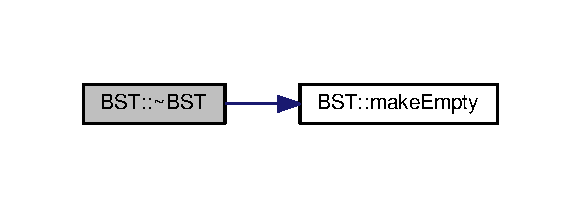
\includegraphics[width=279pt]{classBST_abf3125f968641c8726101c5dd18f36be_cgraph}
\end{center}
\end{figure}




\subsection{Member Function Documentation}
\index{B\+ST@{B\+ST}!find@{find}}
\index{find@{find}!B\+ST@{B\+ST}}
\subsubsection[{\texorpdfstring{find(const Comparable \&x) const }{find(const Comparable &x) const }}]{\setlength{\rightskip}{0pt plus 5cm}template$<$class Comparable$>$ const Comparable \& {\bf B\+ST}$<$ Comparable $>$\+::find (
\begin{DoxyParamCaption}
\item[{const Comparable \&}]{x}
\end{DoxyParamCaption}
) const}\hypertarget{classBST_a337dce7f94a881e253635cbf3ac7eacf}{}\label{classBST_a337dce7f94a881e253635cbf3ac7eacf}

\begin{DoxyCode}
131 \{
132   \textcolor{keywordflow}{return} elementAt( \hyperlink{classBST_a337dce7f94a881e253635cbf3ac7eacf}{find}( x, root ) );
133 \}
\end{DoxyCode}


Here is the caller graph for this function\+:\nopagebreak
\begin{figure}[H]
\begin{center}
\leavevmode
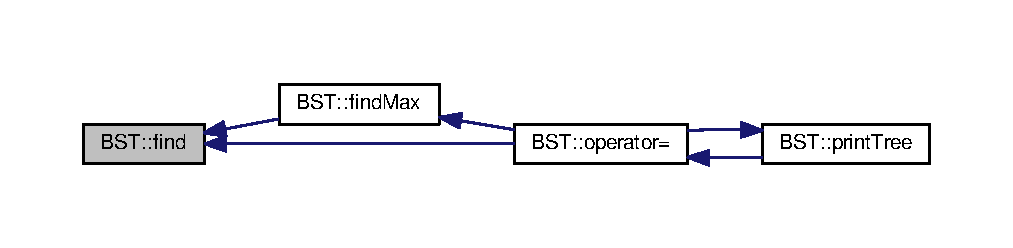
\includegraphics[width=350pt]{classBST_a337dce7f94a881e253635cbf3ac7eacf_icgraph}
\end{center}
\end{figure}


\index{B\+ST@{B\+ST}!find\+Max@{find\+Max}}
\index{find\+Max@{find\+Max}!B\+ST@{B\+ST}}
\subsubsection[{\texorpdfstring{find\+Max() const }{findMax() const }}]{\setlength{\rightskip}{0pt plus 5cm}template$<$class Comparable $>$ const Comparable \& {\bf B\+ST}$<$ Comparable $>$\+::find\+Max (
\begin{DoxyParamCaption}
{}
\end{DoxyParamCaption}
) const}\hypertarget{classBST_aee725fe273c0b3641070883b50eee271}{}\label{classBST_aee725fe273c0b3641070883b50eee271}

\begin{DoxyCode}
124 \{
125   \textcolor{keywordflow}{return} elementAt( \hyperlink{classBST_aee725fe273c0b3641070883b50eee271}{findMax}( root ) );
126 \}
\end{DoxyCode}


Here is the call graph for this function\+:\nopagebreak
\begin{figure}[H]
\begin{center}
\leavevmode
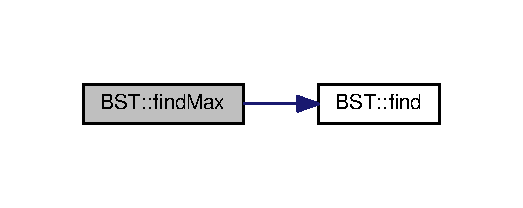
\includegraphics[width=251pt]{classBST_aee725fe273c0b3641070883b50eee271_cgraph}
\end{center}
\end{figure}




Here is the caller graph for this function\+:\nopagebreak
\begin{figure}[H]
\begin{center}
\leavevmode
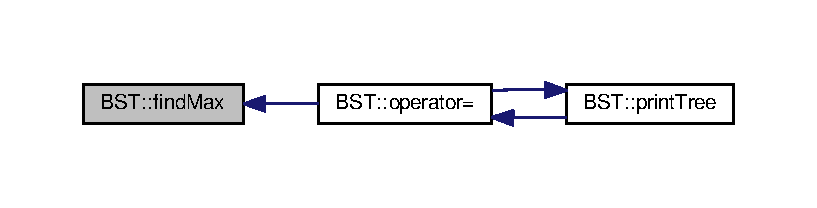
\includegraphics[width=350pt]{classBST_aee725fe273c0b3641070883b50eee271_icgraph}
\end{center}
\end{figure}


\index{B\+ST@{B\+ST}!find\+Min@{find\+Min}}
\index{find\+Min@{find\+Min}!B\+ST@{B\+ST}}
\subsubsection[{\texorpdfstring{find\+Min() const }{findMin() const }}]{\setlength{\rightskip}{0pt plus 5cm}template$<$class Comparable $>$ const Comparable \& {\bf B\+ST}$<$ Comparable $>$\+::find\+Min (
\begin{DoxyParamCaption}
{}
\end{DoxyParamCaption}
) const}\hypertarget{classBST_a34fd17be76f49a77573185f29dede6be}{}\label{classBST_a34fd17be76f49a77573185f29dede6be}

\begin{DoxyCode}
118 \{
119   \textcolor{keywordflow}{return} elementAt( \hyperlink{classBST_a34fd17be76f49a77573185f29dede6be}{findMin}( root ) );
120 \}
\end{DoxyCode}


Here is the caller graph for this function\+:\nopagebreak
\begin{figure}[H]
\begin{center}
\leavevmode
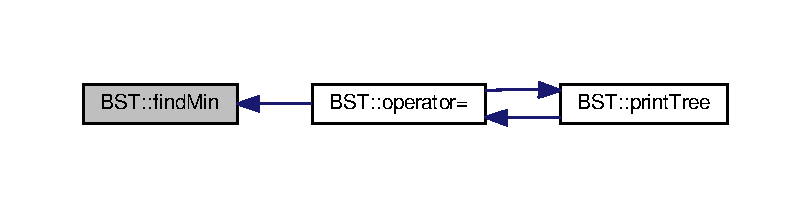
\includegraphics[width=350pt]{classBST_a34fd17be76f49a77573185f29dede6be_icgraph}
\end{center}
\end{figure}


\index{B\+ST@{B\+ST}!insert@{insert}}
\index{insert@{insert}!B\+ST@{B\+ST}}
\subsubsection[{\texorpdfstring{insert(const Comparable \&x)}{insert(const Comparable &x)}}]{\setlength{\rightskip}{0pt plus 5cm}template$<$class Comparable$>$ void {\bf B\+ST}$<$ Comparable $>$\+::insert (
\begin{DoxyParamCaption}
\item[{const Comparable \&}]{x}
\end{DoxyParamCaption}
)}\hypertarget{classBST_a2b117df6521c7d61dac75ff2c938bae7}{}\label{classBST_a2b117df6521c7d61dac75ff2c938bae7}

\begin{DoxyCode}
106 \{
107   \hyperlink{classBST_a2b117df6521c7d61dac75ff2c938bae7}{insert}( x, root );
108 \}
\end{DoxyCode}


Here is the caller graph for this function\+:\nopagebreak
\begin{figure}[H]
\begin{center}
\leavevmode
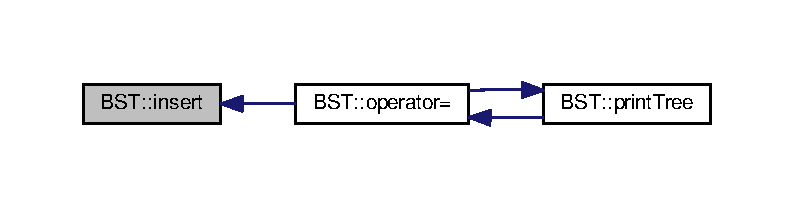
\includegraphics[width=350pt]{classBST_a2b117df6521c7d61dac75ff2c938bae7_icgraph}
\end{center}
\end{figure}


\index{B\+ST@{B\+ST}!is\+Empty@{is\+Empty}}
\index{is\+Empty@{is\+Empty}!B\+ST@{B\+ST}}
\subsubsection[{\texorpdfstring{is\+Empty() const }{isEmpty() const }}]{\setlength{\rightskip}{0pt plus 5cm}template$<$class Comparable $>$ bool {\bf B\+ST}$<$ Comparable $>$\+::is\+Empty (
\begin{DoxyParamCaption}
{}
\end{DoxyParamCaption}
) const}\hypertarget{classBST_a8018fc7d6c15b2564c10ddcc4316c64d}{}\label{classBST_a8018fc7d6c15b2564c10ddcc4316c64d}

\begin{DoxyCode}
143 \{
144   \textcolor{keywordflow}{return} root == NULL;
145 \}
\end{DoxyCode}


Here is the caller graph for this function\+:\nopagebreak
\begin{figure}[H]
\begin{center}
\leavevmode
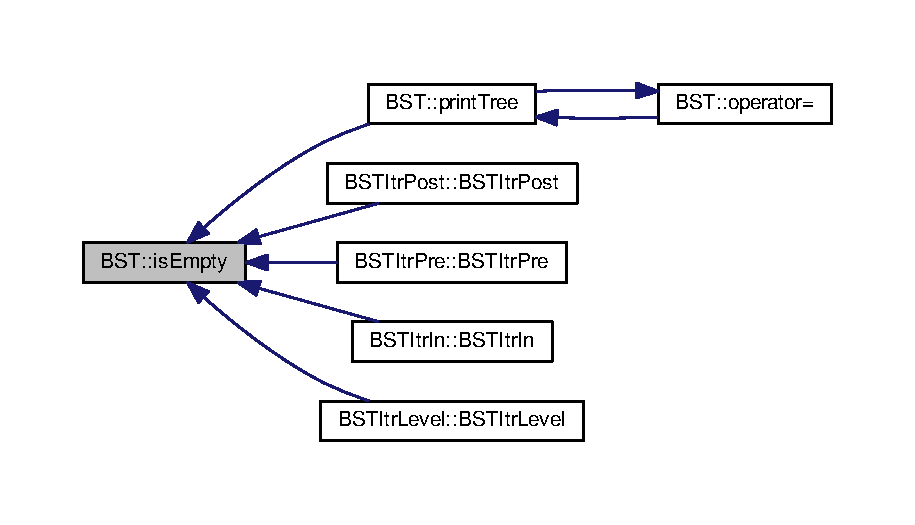
\includegraphics[width=350pt]{classBST_a8018fc7d6c15b2564c10ddcc4316c64d_icgraph}
\end{center}
\end{figure}


\index{B\+ST@{B\+ST}!make\+Empty@{make\+Empty}}
\index{make\+Empty@{make\+Empty}!B\+ST@{B\+ST}}
\subsubsection[{\texorpdfstring{make\+Empty()}{makeEmpty()}}]{\setlength{\rightskip}{0pt plus 5cm}template$<$class Comparable $>$ void {\bf B\+ST}$<$ Comparable $>$\+::make\+Empty (
\begin{DoxyParamCaption}
{}
\end{DoxyParamCaption}
)}\hypertarget{classBST_a050d829503a88714c4ad0773cf6d3af6}{}\label{classBST_a050d829503a88714c4ad0773cf6d3af6}

\begin{DoxyCode}
137 \{
138   \hyperlink{classBST_a050d829503a88714c4ad0773cf6d3af6}{makeEmpty}( root );
139 \}
\end{DoxyCode}


Here is the caller graph for this function\+:\nopagebreak
\begin{figure}[H]
\begin{center}
\leavevmode
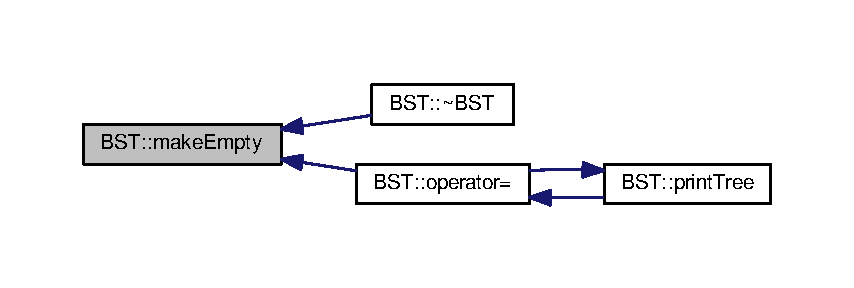
\includegraphics[width=350pt]{classBST_a050d829503a88714c4ad0773cf6d3af6_icgraph}
\end{center}
\end{figure}


\index{B\+ST@{B\+ST}!operator=@{operator=}}
\index{operator=@{operator=}!B\+ST@{B\+ST}}
\subsubsection[{\texorpdfstring{operator=(const B\+S\+T \&rhs)}{operator=(const BST &rhs)}}]{\setlength{\rightskip}{0pt plus 5cm}template$<$class Comparable $>$ const {\bf B\+ST}$<$ Comparable $>$ \& {\bf B\+ST}$<$ Comparable $>$\+::operator= (
\begin{DoxyParamCaption}
\item[{const {\bf B\+ST}$<$ Comparable $>$ \&}]{rhs}
\end{DoxyParamCaption}
)}\hypertarget{classBST_aa80c39f454c89d4a202be3d1445823f3}{}\label{classBST_aa80c39f454c89d4a202be3d1445823f3}

\begin{DoxyCode}
161 \{
162   \textcolor{keywordflow}{if}( \textcolor{keyword}{this} != &rhs )
163     \{
164       \hyperlink{classBST_a050d829503a88714c4ad0773cf6d3af6}{makeEmpty}( );
165       root = clone( rhs.root );
166     \}
167   \textcolor{keywordflow}{return} *\textcolor{keyword}{this};
168 \}
\end{DoxyCode}


Here is the call graph for this function\+:\nopagebreak
\begin{figure}[H]
\begin{center}
\leavevmode
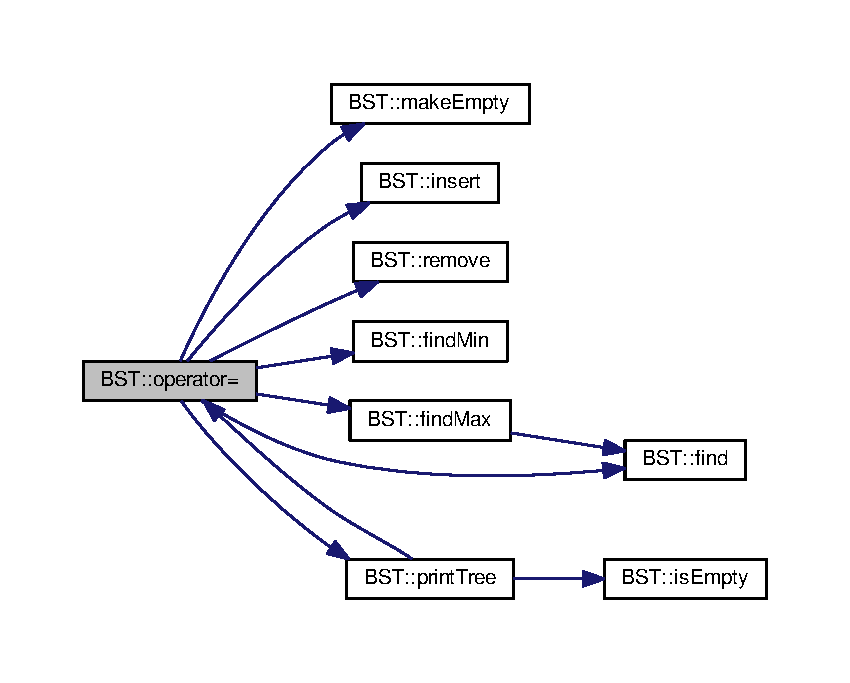
\includegraphics[width=350pt]{classBST_aa80c39f454c89d4a202be3d1445823f3_cgraph}
\end{center}
\end{figure}




Here is the caller graph for this function\+:\nopagebreak
\begin{figure}[H]
\begin{center}
\leavevmode
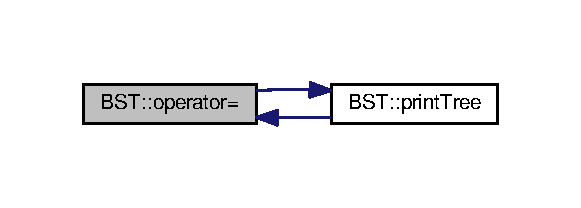
\includegraphics[width=279pt]{classBST_aa80c39f454c89d4a202be3d1445823f3_icgraph}
\end{center}
\end{figure}


\index{B\+ST@{B\+ST}!print\+Tree@{print\+Tree}}
\index{print\+Tree@{print\+Tree}!B\+ST@{B\+ST}}
\subsubsection[{\texorpdfstring{print\+Tree() const }{printTree() const }}]{\setlength{\rightskip}{0pt plus 5cm}template$<$class Comparable $>$ void {\bf B\+ST}$<$ Comparable $>$\+::print\+Tree (
\begin{DoxyParamCaption}
{}
\end{DoxyParamCaption}
) const}\hypertarget{classBST_a5270473db9e17e1737b92dd0d6cd0ee5}{}\label{classBST_a5270473db9e17e1737b92dd0d6cd0ee5}

\begin{DoxyCode}
150 \{
151   \textcolor{keywordflow}{if}( \hyperlink{classBST_a8018fc7d6c15b2564c10ddcc4316c64d}{isEmpty}( ) )
152     cout << \textcolor{stringliteral}{"Empty tree"} << endl;
153   \textcolor{keywordflow}{else}
154     \hyperlink{classBST_a5270473db9e17e1737b92dd0d6cd0ee5}{printTree}( root );
155 \}
\end{DoxyCode}


Here is the call graph for this function\+:\nopagebreak
\begin{figure}[H]
\begin{center}
\leavevmode
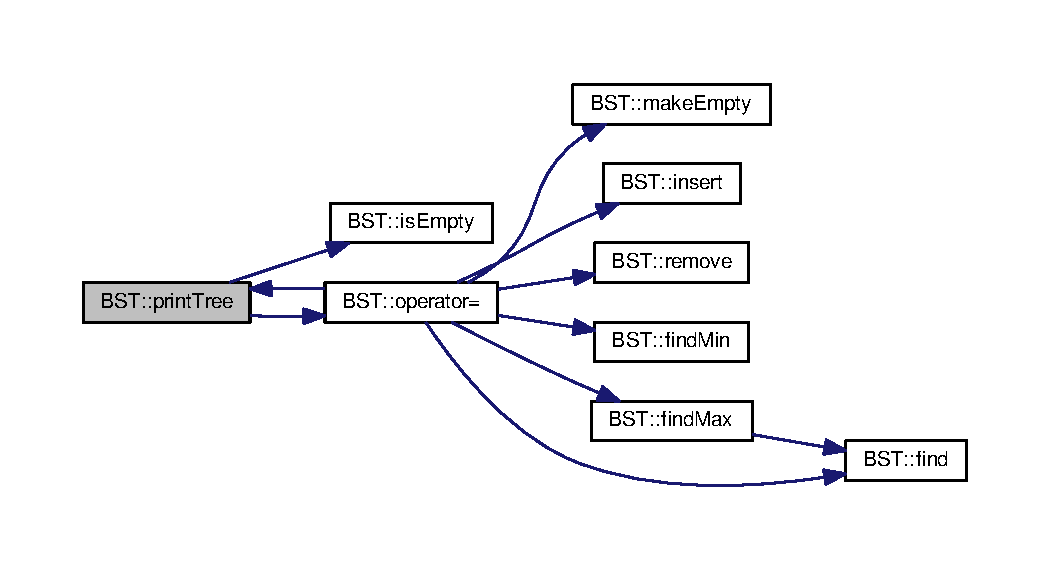
\includegraphics[width=350pt]{classBST_a5270473db9e17e1737b92dd0d6cd0ee5_cgraph}
\end{center}
\end{figure}




Here is the caller graph for this function\+:\nopagebreak
\begin{figure}[H]
\begin{center}
\leavevmode
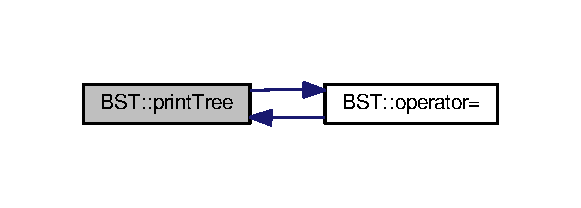
\includegraphics[width=279pt]{classBST_a5270473db9e17e1737b92dd0d6cd0ee5_icgraph}
\end{center}
\end{figure}


\index{B\+ST@{B\+ST}!remove@{remove}}
\index{remove@{remove}!B\+ST@{B\+ST}}
\subsubsection[{\texorpdfstring{remove(const Comparable \&x)}{remove(const Comparable &x)}}]{\setlength{\rightskip}{0pt plus 5cm}template$<$class Comparable$>$ void {\bf B\+ST}$<$ Comparable $>$\+::remove (
\begin{DoxyParamCaption}
\item[{const Comparable \&}]{x}
\end{DoxyParamCaption}
)}\hypertarget{classBST_a6f01a0b44daf82a42022b6eb4c0df7a2}{}\label{classBST_a6f01a0b44daf82a42022b6eb4c0df7a2}

\begin{DoxyCode}
112 \{
113   \textcolor{keyword}{remove}( x, root );
114 \}
\end{DoxyCode}


Here is the caller graph for this function\+:\nopagebreak
\begin{figure}[H]
\begin{center}
\leavevmode
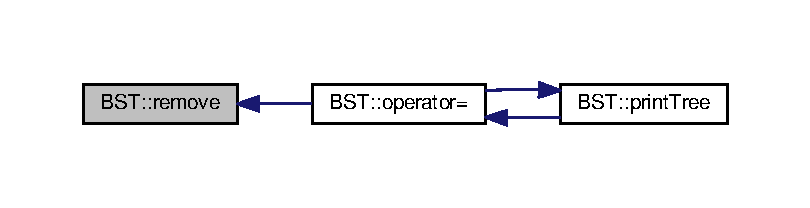
\includegraphics[width=350pt]{classBST_a6f01a0b44daf82a42022b6eb4c0df7a2_icgraph}
\end{center}
\end{figure}




\subsection{Friends And Related Function Documentation}
\index{B\+ST@{B\+ST}!B\+S\+T\+Itr\+In$<$ Comparable $>$@{B\+S\+T\+Itr\+In$<$ Comparable $>$}}
\index{B\+S\+T\+Itr\+In$<$ Comparable $>$@{B\+S\+T\+Itr\+In$<$ Comparable $>$}!B\+ST@{B\+ST}}
\subsubsection[{\texorpdfstring{B\+S\+T\+Itr\+In$<$ Comparable $>$}{BSTItrIn< Comparable >}}]{\setlength{\rightskip}{0pt plus 5cm}template$<$class Comparable$>$ friend class {\bf B\+S\+T\+Itr\+In}$<$ Comparable $>$\hspace{0.3cm}{\ttfamily [friend]}}\hypertarget{classBST_aab3993acac2ab24a0b59edb0c3acc775}{}\label{classBST_aab3993acac2ab24a0b59edb0c3acc775}
\index{B\+ST@{B\+ST}!B\+S\+T\+Itr\+Level$<$ Comparable $>$@{B\+S\+T\+Itr\+Level$<$ Comparable $>$}}
\index{B\+S\+T\+Itr\+Level$<$ Comparable $>$@{B\+S\+T\+Itr\+Level$<$ Comparable $>$}!B\+ST@{B\+ST}}
\subsubsection[{\texorpdfstring{B\+S\+T\+Itr\+Level$<$ Comparable $>$}{BSTItrLevel< Comparable >}}]{\setlength{\rightskip}{0pt plus 5cm}template$<$class Comparable$>$ friend class {\bf B\+S\+T\+Itr\+Level}$<$ Comparable $>$\hspace{0.3cm}{\ttfamily [friend]}}\hypertarget{classBST_a26ff00bc0d87069aed877f10fd3c80a8}{}\label{classBST_a26ff00bc0d87069aed877f10fd3c80a8}
\index{B\+ST@{B\+ST}!B\+S\+T\+Itr\+Post$<$ Comparable $>$@{B\+S\+T\+Itr\+Post$<$ Comparable $>$}}
\index{B\+S\+T\+Itr\+Post$<$ Comparable $>$@{B\+S\+T\+Itr\+Post$<$ Comparable $>$}!B\+ST@{B\+ST}}
\subsubsection[{\texorpdfstring{B\+S\+T\+Itr\+Post$<$ Comparable $>$}{BSTItrPost< Comparable >}}]{\setlength{\rightskip}{0pt plus 5cm}template$<$class Comparable$>$ friend class {\bf B\+S\+T\+Itr\+Post}$<$ Comparable $>$\hspace{0.3cm}{\ttfamily [friend]}}\hypertarget{classBST_a5dc153694be266f6e772659486219da7}{}\label{classBST_a5dc153694be266f6e772659486219da7}
\index{B\+ST@{B\+ST}!B\+S\+T\+Itr\+Pre$<$ Comparable $>$@{B\+S\+T\+Itr\+Pre$<$ Comparable $>$}}
\index{B\+S\+T\+Itr\+Pre$<$ Comparable $>$@{B\+S\+T\+Itr\+Pre$<$ Comparable $>$}!B\+ST@{B\+ST}}
\subsubsection[{\texorpdfstring{B\+S\+T\+Itr\+Pre$<$ Comparable $>$}{BSTItrPre< Comparable >}}]{\setlength{\rightskip}{0pt plus 5cm}template$<$class Comparable$>$ friend class {\bf B\+S\+T\+Itr\+Pre}$<$ Comparable $>$\hspace{0.3cm}{\ttfamily [friend]}}\hypertarget{classBST_a45a55df6f11541416d4ea7684c575c1a}{}\label{classBST_a45a55df6f11541416d4ea7684c575c1a}


The documentation for this class was generated from the following file\+:\begin{DoxyCompactItemize}
\item 
/home/joao/\+Documentos/\+Projetos/\+Porto-\/rivers-\/cruise-\/manager/src/\hyperlink{BST_8h}{B\+S\+T.\+h}\end{DoxyCompactItemize}

\hypertarget{classBSTItrIn}{}\section{B\+S\+T\+Itr\+In$<$ Comparable $>$ Class Template Reference}
\label{classBSTItrIn}\index{B\+S\+T\+Itr\+In$<$ Comparable $>$@{B\+S\+T\+Itr\+In$<$ Comparable $>$}}


{\ttfamily \#include $<$B\+S\+T.\+h$>$}

\subsection*{Public Member Functions}
\begin{DoxyCompactItemize}
\item 
\hyperlink{classBSTItrIn_ac836e2f560fed9cc7ef8e5431a2836cc}{B\+S\+T\+Itr\+In} (const \hyperlink{classBST}{B\+ST}$<$ Comparable $>$ \&bt)
\item 
void \hyperlink{classBSTItrIn_ac772d3ebbac748c5f8cf9bc659f2e32c}{advance} ()
\item 
Comparable \& \hyperlink{classBSTItrIn_ac7ac215c1247bd25fc1fdb8053826a32}{retrieve} ()
\item 
bool \hyperlink{classBSTItrIn_a6f9a43217862c263a9bf15b9a08b889a}{is\+At\+End} ()
\end{DoxyCompactItemize}


\subsection{Constructor \& Destructor Documentation}
\index{B\+S\+T\+Itr\+In@{B\+S\+T\+Itr\+In}!B\+S\+T\+Itr\+In@{B\+S\+T\+Itr\+In}}
\index{B\+S\+T\+Itr\+In@{B\+S\+T\+Itr\+In}!B\+S\+T\+Itr\+In@{B\+S\+T\+Itr\+In}}
\subsubsection[{\texorpdfstring{B\+S\+T\+Itr\+In(const B\+S\+T$<$ Comparable $>$ \&bt)}{BSTItrIn(const BST< Comparable > &bt)}}]{\setlength{\rightskip}{0pt plus 5cm}template$<$class Comparable $>$ {\bf B\+S\+T\+Itr\+In}$<$ Comparable $>$\+::{\bf B\+S\+T\+Itr\+In} (
\begin{DoxyParamCaption}
\item[{const {\bf B\+ST}$<$ Comparable $>$ \&}]{bt}
\end{DoxyParamCaption}
)}\hypertarget{classBSTItrIn_ac836e2f560fed9cc7ef8e5431a2836cc}{}\label{classBSTItrIn_ac836e2f560fed9cc7ef8e5431a2836cc}

\begin{DoxyCode}
431 \{
432   \textcolor{keywordflow}{if} (!bt.\hyperlink{classBST_a8018fc7d6c15b2564c10ddcc4316c64d}{isEmpty}())
433     slideLeft(bt.root);
434 \}
\end{DoxyCode}


Here is the call graph for this function\+:
\nopagebreak
\begin{figure}[H]
\begin{center}
\leavevmode
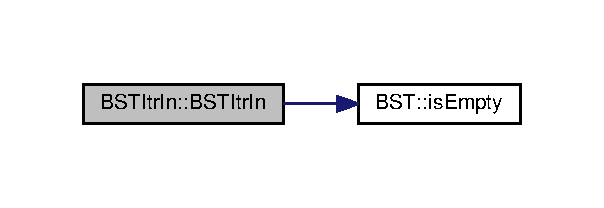
\includegraphics[width=290pt]{classBSTItrIn_ac836e2f560fed9cc7ef8e5431a2836cc_cgraph}
\end{center}
\end{figure}




\subsection{Member Function Documentation}
\index{B\+S\+T\+Itr\+In@{B\+S\+T\+Itr\+In}!advance@{advance}}
\index{advance@{advance}!B\+S\+T\+Itr\+In@{B\+S\+T\+Itr\+In}}
\subsubsection[{\texorpdfstring{advance()}{advance()}}]{\setlength{\rightskip}{0pt plus 5cm}template$<$class Comparable $>$ void {\bf B\+S\+T\+Itr\+In}$<$ Comparable $>$\+::advance (
\begin{DoxyParamCaption}
{}
\end{DoxyParamCaption}
)}\hypertarget{classBSTItrIn_ac772d3ebbac748c5f8cf9bc659f2e32c}{}\label{classBSTItrIn_ac772d3ebbac748c5f8cf9bc659f2e32c}

\begin{DoxyCode}
447 \{
448   \hyperlink{classBinaryNode}{BinaryNode<Comparable>} * actual = itrStack.top();
449   itrStack.pop();
450   \hyperlink{classBinaryNode}{BinaryNode<Comparable>} * seguinte = actual->right;
451   \textcolor{keywordflow}{if} (seguinte)
452     slideLeft(seguinte);
453 \}
\end{DoxyCode}


Here is the caller graph for this function\+:
\nopagebreak
\begin{figure}[H]
\begin{center}
\leavevmode
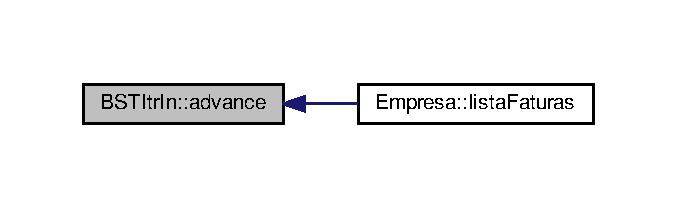
\includegraphics[width=325pt]{classBSTItrIn_ac772d3ebbac748c5f8cf9bc659f2e32c_icgraph}
\end{center}
\end{figure}


\index{B\+S\+T\+Itr\+In@{B\+S\+T\+Itr\+In}!is\+At\+End@{is\+At\+End}}
\index{is\+At\+End@{is\+At\+End}!B\+S\+T\+Itr\+In@{B\+S\+T\+Itr\+In}}
\subsubsection[{\texorpdfstring{is\+At\+End()}{isAtEnd()}}]{\setlength{\rightskip}{0pt plus 5cm}template$<$class Comparable$>$ bool {\bf B\+S\+T\+Itr\+In}$<$ Comparable $>$\+::is\+At\+End (
\begin{DoxyParamCaption}
{}
\end{DoxyParamCaption}
)\hspace{0.3cm}{\ttfamily [inline]}}\hypertarget{classBSTItrIn_a6f9a43217862c263a9bf15b9a08b889a}{}\label{classBSTItrIn_a6f9a43217862c263a9bf15b9a08b889a}

\begin{DoxyCode}
421 \{\textcolor{keywordflow}{return} itrStack.empty(); \}
\end{DoxyCode}


Here is the caller graph for this function\+:
\nopagebreak
\begin{figure}[H]
\begin{center}
\leavevmode
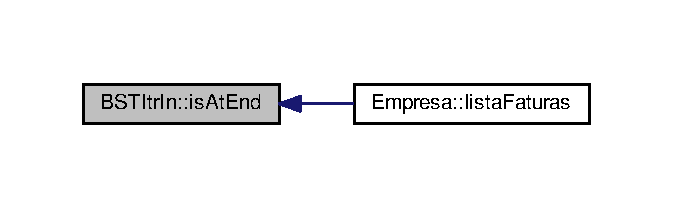
\includegraphics[width=323pt]{classBSTItrIn_a6f9a43217862c263a9bf15b9a08b889a_icgraph}
\end{center}
\end{figure}


\index{B\+S\+T\+Itr\+In@{B\+S\+T\+Itr\+In}!retrieve@{retrieve}}
\index{retrieve@{retrieve}!B\+S\+T\+Itr\+In@{B\+S\+T\+Itr\+In}}
\subsubsection[{\texorpdfstring{retrieve()}{retrieve()}}]{\setlength{\rightskip}{0pt plus 5cm}template$<$class Comparable$>$ Comparable\& {\bf B\+S\+T\+Itr\+In}$<$ Comparable $>$\+::retrieve (
\begin{DoxyParamCaption}
{}
\end{DoxyParamCaption}
)\hspace{0.3cm}{\ttfamily [inline]}}\hypertarget{classBSTItrIn_ac7ac215c1247bd25fc1fdb8053826a32}{}\label{classBSTItrIn_ac7ac215c1247bd25fc1fdb8053826a32}

\begin{DoxyCode}
420 \{ \textcolor{keywordflow}{return} itrStack.top()->element; \}
\end{DoxyCode}


Here is the caller graph for this function\+:
\nopagebreak
\begin{figure}[H]
\begin{center}
\leavevmode
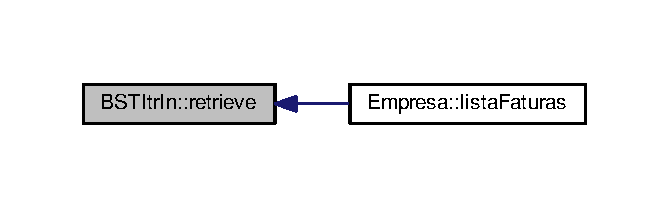
\includegraphics[width=321pt]{classBSTItrIn_ac7ac215c1247bd25fc1fdb8053826a32_icgraph}
\end{center}
\end{figure}




The documentation for this class was generated from the following file\+:\begin{DoxyCompactItemize}
\item 
/home/joao/\+Documentos/\+Projetos/\+Porto-\/rivers-\/cruise-\/manager/src/\hyperlink{BST_8h}{B\+S\+T.\+h}\end{DoxyCompactItemize}

\hypertarget{classBSTItrLevel}{}\section{B\+S\+T\+Itr\+Level$<$ Comparable $>$ Class Template Reference}
\label{classBSTItrLevel}\index{B\+S\+T\+Itr\+Level$<$ Comparable $>$@{B\+S\+T\+Itr\+Level$<$ Comparable $>$}}


{\ttfamily \#include $<$B\+S\+T.\+h$>$}

\subsection*{Public Member Functions}
\begin{DoxyCompactItemize}
\item 
\hyperlink{classBSTItrLevel_a8fd5cdde93eb182c4cd5cf6b2c5efaeb}{B\+S\+T\+Itr\+Level} (const \hyperlink{classBST}{B\+ST}$<$ Comparable $>$ \&bt)
\item 
void \hyperlink{classBSTItrLevel_ad54a6fa289a59d6050b507abe40d463b}{advance} ()
\item 
Comparable \& \hyperlink{classBSTItrLevel_a0340bd9f21f72ae25348f383e67e7f91}{retrieve} ()
\item 
bool \hyperlink{classBSTItrLevel_a89bc8e81dde255fd6bad917cacc0d489}{is\+At\+End} ()
\end{DoxyCompactItemize}


\subsection{Constructor \& Destructor Documentation}
\index{B\+S\+T\+Itr\+Level@{B\+S\+T\+Itr\+Level}!B\+S\+T\+Itr\+Level@{B\+S\+T\+Itr\+Level}}
\index{B\+S\+T\+Itr\+Level@{B\+S\+T\+Itr\+Level}!B\+S\+T\+Itr\+Level@{B\+S\+T\+Itr\+Level}}
\subsubsection[{\texorpdfstring{B\+S\+T\+Itr\+Level(const B\+S\+T$<$ Comparable $>$ \&bt)}{BSTItrLevel(const BST< Comparable > &bt)}}]{\setlength{\rightskip}{0pt plus 5cm}template$<$class Comparable $>$ {\bf B\+S\+T\+Itr\+Level}$<$ Comparable $>$\+::{\bf B\+S\+T\+Itr\+Level} (
\begin{DoxyParamCaption}
\item[{const {\bf B\+ST}$<$ Comparable $>$ \&}]{bt}
\end{DoxyParamCaption}
)}\hypertarget{classBSTItrLevel_a8fd5cdde93eb182c4cd5cf6b2c5efaeb}{}\label{classBSTItrLevel_a8fd5cdde93eb182c4cd5cf6b2c5efaeb}

\begin{DoxyCode}
472 \{
473   \textcolor{keywordflow}{if} (!bt.\hyperlink{classBST_a8018fc7d6c15b2564c10ddcc4316c64d}{isEmpty}())
474     itrQueue.push(bt.root);
475 \}
\end{DoxyCode}


Here is the call graph for this function\+:
\nopagebreak
\begin{figure}[H]
\begin{center}
\leavevmode
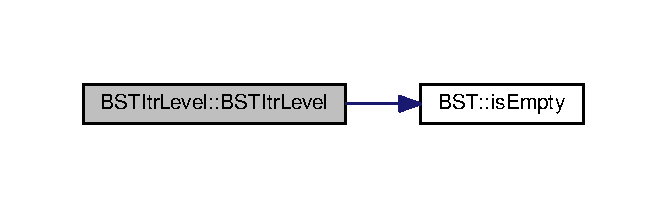
\includegraphics[width=320pt]{classBSTItrLevel_a8fd5cdde93eb182c4cd5cf6b2c5efaeb_cgraph}
\end{center}
\end{figure}




\subsection{Member Function Documentation}
\index{B\+S\+T\+Itr\+Level@{B\+S\+T\+Itr\+Level}!advance@{advance}}
\index{advance@{advance}!B\+S\+T\+Itr\+Level@{B\+S\+T\+Itr\+Level}}
\subsubsection[{\texorpdfstring{advance()}{advance()}}]{\setlength{\rightskip}{0pt plus 5cm}template$<$class Comparable $>$ void {\bf B\+S\+T\+Itr\+Level}$<$ Comparable $>$\+::advance (
\begin{DoxyParamCaption}
{}
\end{DoxyParamCaption}
)}\hypertarget{classBSTItrLevel_ad54a6fa289a59d6050b507abe40d463b}{}\label{classBSTItrLevel_ad54a6fa289a59d6050b507abe40d463b}

\begin{DoxyCode}
479 \{
480   \hyperlink{classBinaryNode}{BinaryNode<Comparable>} * actual = itrQueue.front();
481   itrQueue.pop();
482   \hyperlink{classBinaryNode}{BinaryNode<Comparable>} * seguinte = actual->left;
483   \textcolor{keywordflow}{if} (seguinte)
484     itrQueue.push(seguinte);
485   seguinte = actual->right;
486   \textcolor{keywordflow}{if} (seguinte)
487     itrQueue.push(seguinte);
488 \}
\end{DoxyCode}
\index{B\+S\+T\+Itr\+Level@{B\+S\+T\+Itr\+Level}!is\+At\+End@{is\+At\+End}}
\index{is\+At\+End@{is\+At\+End}!B\+S\+T\+Itr\+Level@{B\+S\+T\+Itr\+Level}}
\subsubsection[{\texorpdfstring{is\+At\+End()}{isAtEnd()}}]{\setlength{\rightskip}{0pt plus 5cm}template$<$class Comparable $>$ bool {\bf B\+S\+T\+Itr\+Level}$<$ Comparable $>$\+::is\+At\+End (
\begin{DoxyParamCaption}
{}
\end{DoxyParamCaption}
)\hspace{0.3cm}{\ttfamily [inline]}}\hypertarget{classBSTItrLevel_a89bc8e81dde255fd6bad917cacc0d489}{}\label{classBSTItrLevel_a89bc8e81dde255fd6bad917cacc0d489}

\begin{DoxyCode}
463 \{\textcolor{keywordflow}{return} itrQueue.empty(); \}
\end{DoxyCode}
\index{B\+S\+T\+Itr\+Level@{B\+S\+T\+Itr\+Level}!retrieve@{retrieve}}
\index{retrieve@{retrieve}!B\+S\+T\+Itr\+Level@{B\+S\+T\+Itr\+Level}}
\subsubsection[{\texorpdfstring{retrieve()}{retrieve()}}]{\setlength{\rightskip}{0pt plus 5cm}template$<$class Comparable $>$ Comparable\& {\bf B\+S\+T\+Itr\+Level}$<$ Comparable $>$\+::retrieve (
\begin{DoxyParamCaption}
{}
\end{DoxyParamCaption}
)\hspace{0.3cm}{\ttfamily [inline]}}\hypertarget{classBSTItrLevel_a0340bd9f21f72ae25348f383e67e7f91}{}\label{classBSTItrLevel_a0340bd9f21f72ae25348f383e67e7f91}

\begin{DoxyCode}
462 \{ \textcolor{keywordflow}{return} itrQueue.front()->element; \}
\end{DoxyCode}


The documentation for this class was generated from the following file\+:\begin{DoxyCompactItemize}
\item 
/home/joao/\+Documentos/\+Projetos/\+Porto-\/rivers-\/cruise-\/manager/src/\hyperlink{BST_8h}{B\+S\+T.\+h}\end{DoxyCompactItemize}

\hypertarget{classBSTItrPost}{}\section{B\+S\+T\+Itr\+Post$<$ Comparable $>$ Class Template Reference}
\label{classBSTItrPost}\index{B\+S\+T\+Itr\+Post$<$ Comparable $>$@{B\+S\+T\+Itr\+Post$<$ Comparable $>$}}


{\ttfamily \#include $<$B\+S\+T.\+h$>$}

\subsection*{Public Member Functions}
\begin{DoxyCompactItemize}
\item 
\hyperlink{classBSTItrPost_acf7e537dea01978f40c40909c55c56c2}{B\+S\+T\+Itr\+Post} (const \hyperlink{classBST}{B\+ST}$<$ Comparable $>$ \&bt)
\item 
void \hyperlink{classBSTItrPost_a376098e5a82cd02118dd4dcdec49bb26}{advance} ()
\item 
Comparable \& \hyperlink{classBSTItrPost_a72446e4d0df0bcafc14294a78faeb56e}{retrieve} ()
\item 
bool \hyperlink{classBSTItrPost_a2f330e73bb817e8bd1c797805e66ddb7}{is\+At\+End} ()
\end{DoxyCompactItemize}


\subsection{Constructor \& Destructor Documentation}
\index{B\+S\+T\+Itr\+Post@{B\+S\+T\+Itr\+Post}!B\+S\+T\+Itr\+Post@{B\+S\+T\+Itr\+Post}}
\index{B\+S\+T\+Itr\+Post@{B\+S\+T\+Itr\+Post}!B\+S\+T\+Itr\+Post@{B\+S\+T\+Itr\+Post}}
\subsubsection[{\texorpdfstring{B\+S\+T\+Itr\+Post(const B\+S\+T$<$ Comparable $>$ \&bt)}{BSTItrPost(const BST< Comparable > &bt)}}]{\setlength{\rightskip}{0pt plus 5cm}template$<$class Comparable $>$ {\bf B\+S\+T\+Itr\+Post}$<$ Comparable $>$\+::{\bf B\+S\+T\+Itr\+Post} (
\begin{DoxyParamCaption}
\item[{const {\bf B\+ST}$<$ Comparable $>$ \&}]{bt}
\end{DoxyParamCaption}
)}\hypertarget{classBSTItrPost_acf7e537dea01978f40c40909c55c56c2}{}\label{classBSTItrPost_acf7e537dea01978f40c40909c55c56c2}

\begin{DoxyCode}
334 \{
335   \textcolor{keywordflow}{if} (!bt.\hyperlink{classBST_a8018fc7d6c15b2564c10ddcc4316c64d}{isEmpty}())
336     slideDown(bt.root);
337 \}
\end{DoxyCode}


Here is the call graph for this function\+:\nopagebreak
\begin{figure}[H]
\begin{center}
\leavevmode
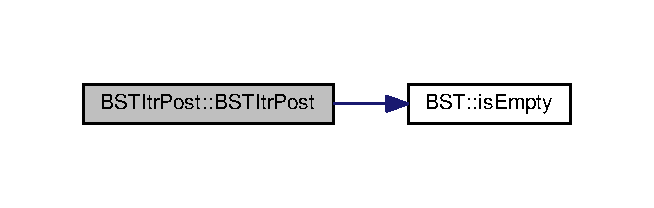
\includegraphics[width=314pt]{classBSTItrPost_acf7e537dea01978f40c40909c55c56c2_cgraph}
\end{center}
\end{figure}




\subsection{Member Function Documentation}
\index{B\+S\+T\+Itr\+Post@{B\+S\+T\+Itr\+Post}!advance@{advance}}
\index{advance@{advance}!B\+S\+T\+Itr\+Post@{B\+S\+T\+Itr\+Post}}
\subsubsection[{\texorpdfstring{advance()}{advance()}}]{\setlength{\rightskip}{0pt plus 5cm}template$<$class Comparable $>$ void {\bf B\+S\+T\+Itr\+Post}$<$ Comparable $>$\+::advance (
\begin{DoxyParamCaption}
{}
\end{DoxyParamCaption}
)}\hypertarget{classBSTItrPost_a376098e5a82cd02118dd4dcdec49bb26}{}\label{classBSTItrPost_a376098e5a82cd02118dd4dcdec49bb26}

\begin{DoxyCode}
341 \{
342   itrStack.pop();
343   visitStack.pop();
344   \textcolor{keywordflow}{if} ((!itrStack.empty()) && (visitStack.top() == \textcolor{keyword}{false})) \{
345     visitStack.pop();
346     visitStack.push(\textcolor{keyword}{true});
347     slideDown(itrStack.top()->right);
348   \}
349 \}
\end{DoxyCode}
\index{B\+S\+T\+Itr\+Post@{B\+S\+T\+Itr\+Post}!is\+At\+End@{is\+At\+End}}
\index{is\+At\+End@{is\+At\+End}!B\+S\+T\+Itr\+Post@{B\+S\+T\+Itr\+Post}}
\subsubsection[{\texorpdfstring{is\+At\+End()}{isAtEnd()}}]{\setlength{\rightskip}{0pt plus 5cm}template$<$class Comparable $>$ bool {\bf B\+S\+T\+Itr\+Post}$<$ Comparable $>$\+::is\+At\+End (
\begin{DoxyParamCaption}
{}
\end{DoxyParamCaption}
)\hspace{0.3cm}{\ttfamily [inline]}}\hypertarget{classBSTItrPost_a2f330e73bb817e8bd1c797805e66ddb7}{}\label{classBSTItrPost_a2f330e73bb817e8bd1c797805e66ddb7}

\begin{DoxyCode}
323 \{\textcolor{keywordflow}{return} itrStack.empty(); \}
\end{DoxyCode}
\index{B\+S\+T\+Itr\+Post@{B\+S\+T\+Itr\+Post}!retrieve@{retrieve}}
\index{retrieve@{retrieve}!B\+S\+T\+Itr\+Post@{B\+S\+T\+Itr\+Post}}
\subsubsection[{\texorpdfstring{retrieve()}{retrieve()}}]{\setlength{\rightskip}{0pt plus 5cm}template$<$class Comparable $>$ Comparable\& {\bf B\+S\+T\+Itr\+Post}$<$ Comparable $>$\+::retrieve (
\begin{DoxyParamCaption}
{}
\end{DoxyParamCaption}
)\hspace{0.3cm}{\ttfamily [inline]}}\hypertarget{classBSTItrPost_a72446e4d0df0bcafc14294a78faeb56e}{}\label{classBSTItrPost_a72446e4d0df0bcafc14294a78faeb56e}

\begin{DoxyCode}
322 \{ \textcolor{keywordflow}{return} itrStack.top()->element; \}
\end{DoxyCode}


The documentation for this class was generated from the following file\+:\begin{DoxyCompactItemize}
\item 
/home/joao/\+Documentos/\+Projetos/\+Porto-\/rivers-\/cruise-\/manager/src/\hyperlink{BST_8h}{B\+S\+T.\+h}\end{DoxyCompactItemize}

\hypertarget{classBSTItrPre}{}\section{B\+S\+T\+Itr\+Pre$<$ Comparable $>$ Class Template Reference}
\label{classBSTItrPre}\index{B\+S\+T\+Itr\+Pre$<$ Comparable $>$@{B\+S\+T\+Itr\+Pre$<$ Comparable $>$}}


{\ttfamily \#include $<$B\+S\+T.\+h$>$}

\subsection*{Public Member Functions}
\begin{DoxyCompactItemize}
\item 
\hyperlink{classBSTItrPre_a11b1cd4e783f153b9c1b64ce2ec8077e}{B\+S\+T\+Itr\+Pre} (const \hyperlink{classBST}{B\+ST}$<$ Comparable $>$ \&bt)
\item 
void \hyperlink{classBSTItrPre_a7a743d66a842018fd833fb2b0737254d}{advance} ()
\item 
Comparable \& \hyperlink{classBSTItrPre_af40033e97f63bf025c2e33a9fdce4c43}{retrieve} ()
\item 
bool \hyperlink{classBSTItrPre_ae282a7b9ffa9d250bb0f6a6d79f6e8d0}{is\+At\+End} ()
\end{DoxyCompactItemize}


\subsection{Constructor \& Destructor Documentation}
\index{B\+S\+T\+Itr\+Pre@{B\+S\+T\+Itr\+Pre}!B\+S\+T\+Itr\+Pre@{B\+S\+T\+Itr\+Pre}}
\index{B\+S\+T\+Itr\+Pre@{B\+S\+T\+Itr\+Pre}!B\+S\+T\+Itr\+Pre@{B\+S\+T\+Itr\+Pre}}
\subsubsection[{\texorpdfstring{B\+S\+T\+Itr\+Pre(const B\+S\+T$<$ Comparable $>$ \&bt)}{BSTItrPre(const BST< Comparable > &bt)}}]{\setlength{\rightskip}{0pt plus 5cm}template$<$class Comparable $>$ {\bf B\+S\+T\+Itr\+Pre}$<$ Comparable $>$\+::{\bf B\+S\+T\+Itr\+Pre} (
\begin{DoxyParamCaption}
\item[{const {\bf B\+ST}$<$ Comparable $>$ \&}]{bt}
\end{DoxyParamCaption}
)}\hypertarget{classBSTItrPre_a11b1cd4e783f153b9c1b64ce2ec8077e}{}\label{classBSTItrPre_a11b1cd4e783f153b9c1b64ce2ec8077e}

\begin{DoxyCode}
388 \{
389   \textcolor{keywordflow}{if} (!bt.\hyperlink{classBST_a8018fc7d6c15b2564c10ddcc4316c64d}{isEmpty}())
390     itrStack.push(bt.root);
391 \}
\end{DoxyCode}


Here is the call graph for this function\+:\nopagebreak
\begin{figure}[H]
\begin{center}
\leavevmode
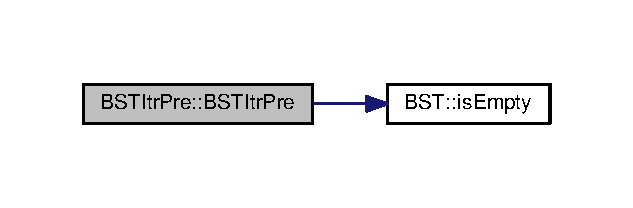
\includegraphics[width=304pt]{classBSTItrPre_a11b1cd4e783f153b9c1b64ce2ec8077e_cgraph}
\end{center}
\end{figure}




\subsection{Member Function Documentation}
\index{B\+S\+T\+Itr\+Pre@{B\+S\+T\+Itr\+Pre}!advance@{advance}}
\index{advance@{advance}!B\+S\+T\+Itr\+Pre@{B\+S\+T\+Itr\+Pre}}
\subsubsection[{\texorpdfstring{advance()}{advance()}}]{\setlength{\rightskip}{0pt plus 5cm}template$<$class Comparable $>$ void {\bf B\+S\+T\+Itr\+Pre}$<$ Comparable $>$\+::advance (
\begin{DoxyParamCaption}
{}
\end{DoxyParamCaption}
)}\hypertarget{classBSTItrPre_a7a743d66a842018fd833fb2b0737254d}{}\label{classBSTItrPre_a7a743d66a842018fd833fb2b0737254d}

\begin{DoxyCode}
395 \{
396   \hyperlink{classBinaryNode}{BinaryNode<Comparable>} * actual = itrStack.top();
397   \hyperlink{classBinaryNode}{BinaryNode<Comparable>} * seguinte = actual->left;
398   \textcolor{keywordflow}{if} (seguinte)
399     itrStack.push(seguinte);
400   \textcolor{keywordflow}{else} \{
401     \textcolor{keywordflow}{while} (!itrStack.empty()) \{
402       actual = itrStack.top();
403       itrStack.pop();
404       seguinte = actual -> right;
405       \textcolor{keywordflow}{if} (seguinte) \{
406     itrStack.push(seguinte);
407     \textcolor{keywordflow}{break};
408       \}
409     \}
410   \}
411 \}
\end{DoxyCode}
\index{B\+S\+T\+Itr\+Pre@{B\+S\+T\+Itr\+Pre}!is\+At\+End@{is\+At\+End}}
\index{is\+At\+End@{is\+At\+End}!B\+S\+T\+Itr\+Pre@{B\+S\+T\+Itr\+Pre}}
\subsubsection[{\texorpdfstring{is\+At\+End()}{isAtEnd()}}]{\setlength{\rightskip}{0pt plus 5cm}template$<$class Comparable $>$ bool {\bf B\+S\+T\+Itr\+Pre}$<$ Comparable $>$\+::is\+At\+End (
\begin{DoxyParamCaption}
{}
\end{DoxyParamCaption}
)\hspace{0.3cm}{\ttfamily [inline]}}\hypertarget{classBSTItrPre_ae282a7b9ffa9d250bb0f6a6d79f6e8d0}{}\label{classBSTItrPre_ae282a7b9ffa9d250bb0f6a6d79f6e8d0}

\begin{DoxyCode}
379 \{\textcolor{keywordflow}{return} itrStack.empty(); \}
\end{DoxyCode}
\index{B\+S\+T\+Itr\+Pre@{B\+S\+T\+Itr\+Pre}!retrieve@{retrieve}}
\index{retrieve@{retrieve}!B\+S\+T\+Itr\+Pre@{B\+S\+T\+Itr\+Pre}}
\subsubsection[{\texorpdfstring{retrieve()}{retrieve()}}]{\setlength{\rightskip}{0pt plus 5cm}template$<$class Comparable $>$ Comparable\& {\bf B\+S\+T\+Itr\+Pre}$<$ Comparable $>$\+::retrieve (
\begin{DoxyParamCaption}
{}
\end{DoxyParamCaption}
)\hspace{0.3cm}{\ttfamily [inline]}}\hypertarget{classBSTItrPre_af40033e97f63bf025c2e33a9fdce4c43}{}\label{classBSTItrPre_af40033e97f63bf025c2e33a9fdce4c43}

\begin{DoxyCode}
378 \{ \textcolor{keywordflow}{return} itrStack.top()->element; \}
\end{DoxyCode}


The documentation for this class was generated from the following file\+:\begin{DoxyCompactItemize}
\item 
/home/joao/\+Documentos/\+Projetos/\+Porto-\/rivers-\/cruise-\/manager/src/\hyperlink{BST_8h}{B\+S\+T.\+h}\end{DoxyCompactItemize}

\hypertarget{classCliente}{}\section{Cliente Class Reference}
\label{classCliente}\index{Cliente@{Cliente}}


{\ttfamily \#include $<$cruise.\+h$>$}

Inheritance diagram for Cliente\+:\begin{figure}[H]
\begin{center}
\leavevmode
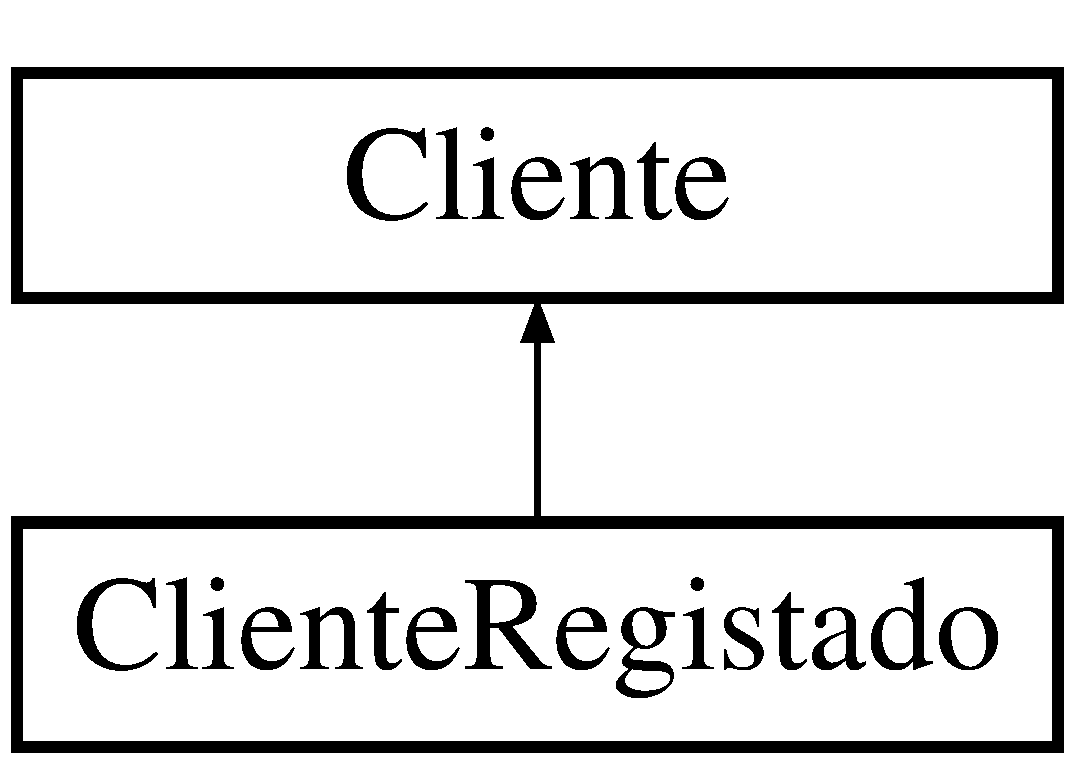
\includegraphics[height=2.000000cm]{classCliente}
\end{center}
\end{figure}
\subsection*{Public Member Functions}
\begin{DoxyCompactItemize}
\item 
\hyperlink{classCliente_a17e05e34ce319b738fb68c53e4ded2c3}{Cliente} (std\+::string \hyperlink{classCliente_aaa79b0a26f7d5d007fe4ae9696564ca5}{nome})
\item 
std\+::string \hyperlink{classCliente_a09b99b4140f32bdd3bf486cc2ac5ee27}{get\+Nome} ()
\item 
virtual unsigned int \hyperlink{classCliente_a4bcd51f0d9a0bfe7d9d47074ac4e65de}{get\+Pontos} ()
\item 
virtual bool \hyperlink{classCliente_acb60d8bf04134b986ae56a79db8beaaf}{is\+Registado} ()
\end{DoxyCompactItemize}
\subsection*{Protected Attributes}
\begin{DoxyCompactItemize}
\item 
std\+::string \hyperlink{classCliente_aaa79b0a26f7d5d007fe4ae9696564ca5}{nome}
\end{DoxyCompactItemize}


\subsection{Constructor \& Destructor Documentation}
\mbox{\Hypertarget{classCliente_a17e05e34ce319b738fb68c53e4ded2c3}\label{classCliente_a17e05e34ce319b738fb68c53e4ded2c3}} 
\index{Cliente@{Cliente}!Cliente@{Cliente}}
\index{Cliente@{Cliente}!Cliente@{Cliente}}
\subsubsection{\texorpdfstring{Cliente()}{Cliente()}}
{\footnotesize\ttfamily Cliente\+::\+Cliente (\begin{DoxyParamCaption}\item[{std\+::string}]{nome }\end{DoxyParamCaption})}



\subsection{Member Function Documentation}
\mbox{\Hypertarget{classCliente_a09b99b4140f32bdd3bf486cc2ac5ee27}\label{classCliente_a09b99b4140f32bdd3bf486cc2ac5ee27}} 
\index{Cliente@{Cliente}!get\+Nome@{get\+Nome}}
\index{get\+Nome@{get\+Nome}!Cliente@{Cliente}}
\subsubsection{\texorpdfstring{get\+Nome()}{getNome()}}
{\footnotesize\ttfamily std\+::string Cliente\+::get\+Nome (\begin{DoxyParamCaption}{ }\end{DoxyParamCaption})\hspace{0.3cm}{\ttfamily [inline]}}

\mbox{\Hypertarget{classCliente_a4bcd51f0d9a0bfe7d9d47074ac4e65de}\label{classCliente_a4bcd51f0d9a0bfe7d9d47074ac4e65de}} 
\index{Cliente@{Cliente}!get\+Pontos@{get\+Pontos}}
\index{get\+Pontos@{get\+Pontos}!Cliente@{Cliente}}
\subsubsection{\texorpdfstring{get\+Pontos()}{getPontos()}}
{\footnotesize\ttfamily virtual unsigned int Cliente\+::get\+Pontos (\begin{DoxyParamCaption}{ }\end{DoxyParamCaption})\hspace{0.3cm}{\ttfamily [inline]}, {\ttfamily [virtual]}}



Reimplemented in \hyperlink{classClienteRegistado_a0118e31f16e4dce542f5e1d124d26c61}{Cliente\+Registado}.

\mbox{\Hypertarget{classCliente_acb60d8bf04134b986ae56a79db8beaaf}\label{classCliente_acb60d8bf04134b986ae56a79db8beaaf}} 
\index{Cliente@{Cliente}!is\+Registado@{is\+Registado}}
\index{is\+Registado@{is\+Registado}!Cliente@{Cliente}}
\subsubsection{\texorpdfstring{is\+Registado()}{isRegistado()}}
{\footnotesize\ttfamily virtual bool Cliente\+::is\+Registado (\begin{DoxyParamCaption}{ }\end{DoxyParamCaption})\hspace{0.3cm}{\ttfamily [inline]}, {\ttfamily [virtual]}}



Reimplemented in \hyperlink{classClienteRegistado_a3dade20423acb0e84c9fbe30c75f0e3e}{Cliente\+Registado}.



\subsection{Member Data Documentation}
\mbox{\Hypertarget{classCliente_aaa79b0a26f7d5d007fe4ae9696564ca5}\label{classCliente_aaa79b0a26f7d5d007fe4ae9696564ca5}} 
\index{Cliente@{Cliente}!nome@{nome}}
\index{nome@{nome}!Cliente@{Cliente}}
\subsubsection{\texorpdfstring{nome}{nome}}
{\footnotesize\ttfamily std\+::string Cliente\+::nome\hspace{0.3cm}{\ttfamily [protected]}}



The documentation for this class was generated from the following files\+:\begin{DoxyCompactItemize}
\item 
/home/joao/\+Documentos/\+Projectos/\+Porto-\/rivers-\/cruise-\/manager/src/\hyperlink{cruise_8h}{cruise.\+h}\item 
/home/joao/\+Documentos/\+Projectos/\+Porto-\/rivers-\/cruise-\/manager/src/\hyperlink{cruise_8cpp}{cruise.\+cpp}\end{DoxyCompactItemize}

\hypertarget{classClienteInativo}{}\section{Cliente\+Inativo Class Reference}
\label{classClienteInativo}\index{Cliente\+Inativo@{Cliente\+Inativo}}


Class for inactive clients.  




{\ttfamily \#include $<$cruise.\+h$>$}

\subsection*{Public Member Functions}
\begin{DoxyCompactItemize}
\item 
\hyperlink{classClienteInativo_a89308172bb87ed33261ab3f0543b407d}{Cliente\+Inativo} (\hyperlink{classCliente}{Cliente} $\ast$ptr)
\begin{DoxyCompactList}\small\item\em Contructs the inactive client object. \end{DoxyCompactList}\item 
std\+::string \hyperlink{classClienteInativo_a0d29faf815a74d59a7f3e4028d5aad2a}{get\+Nome} () const 
\begin{DoxyCompactList}\small\item\em Gets the name. \end{DoxyCompactList}\item 
std\+::string \hyperlink{classClienteInativo_ad7bb77ba3d2752dc916fdc7072846969}{get\+Morada} () const 
\begin{DoxyCompactList}\small\item\em Gets the address. \end{DoxyCompactList}\item 
void \hyperlink{classClienteInativo_aea3df2299f33ea2f4e22f406ba73d5b2}{set\+Morada} (std\+::string nova\+Morada)
\begin{DoxyCompactList}\small\item\em Sets the address. \end{DoxyCompactList}\end{DoxyCompactItemize}


\subsection{Detailed Description}
Class for inactive clients. 

\subsection{Constructor \& Destructor Documentation}
\index{Cliente\+Inativo@{Cliente\+Inativo}!Cliente\+Inativo@{Cliente\+Inativo}}
\index{Cliente\+Inativo@{Cliente\+Inativo}!Cliente\+Inativo@{Cliente\+Inativo}}
\subsubsection[{\texorpdfstring{Cliente\+Inativo(\+Cliente $\ast$ptr)}{ClienteInativo(Cliente *ptr)}}]{\setlength{\rightskip}{0pt plus 5cm}Cliente\+Inativo\+::\+Cliente\+Inativo (
\begin{DoxyParamCaption}
\item[{{\bf Cliente} $\ast$}]{ptr}
\end{DoxyParamCaption}
)}\hypertarget{classClienteInativo_a89308172bb87ed33261ab3f0543b407d}{}\label{classClienteInativo_a89308172bb87ed33261ab3f0543b407d}


Contructs the inactive client object. 


\begin{DoxyParams}{Parameters}
{\em ptr} & The pointer \\
\hline
\end{DoxyParams}

\begin{DoxyCode}
481 : ptr(ptr)\{\}
\end{DoxyCode}


\subsection{Member Function Documentation}
\index{Cliente\+Inativo@{Cliente\+Inativo}!get\+Morada@{get\+Morada}}
\index{get\+Morada@{get\+Morada}!Cliente\+Inativo@{Cliente\+Inativo}}
\subsubsection[{\texorpdfstring{get\+Morada() const }{getMorada() const }}]{\setlength{\rightskip}{0pt plus 5cm}string Cliente\+Inativo\+::get\+Morada (
\begin{DoxyParamCaption}
{}
\end{DoxyParamCaption}
) const}\hypertarget{classClienteInativo_ad7bb77ba3d2752dc916fdc7072846969}{}\label{classClienteInativo_ad7bb77ba3d2752dc916fdc7072846969}


Gets the address. 

\begin{DoxyReturn}{Returns}
The address 
\end{DoxyReturn}

\begin{DoxyCode}
487                                       \{
488     \textcolor{keywordflow}{return} this->ptr->\hyperlink{classCliente_a7f69a0a6ffad90dc0282d7dd9d5cb994}{getMorada}();
489 \}
\end{DoxyCode}


Here is the call graph for this function\+:\nopagebreak
\begin{figure}[H]
\begin{center}
\leavevmode
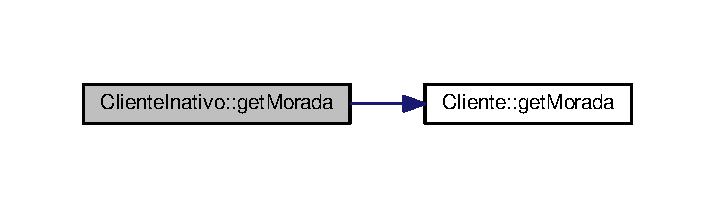
\includegraphics[width=343pt]{classClienteInativo_ad7bb77ba3d2752dc916fdc7072846969_cgraph}
\end{center}
\end{figure}


\index{Cliente\+Inativo@{Cliente\+Inativo}!get\+Nome@{get\+Nome}}
\index{get\+Nome@{get\+Nome}!Cliente\+Inativo@{Cliente\+Inativo}}
\subsubsection[{\texorpdfstring{get\+Nome() const }{getNome() const }}]{\setlength{\rightskip}{0pt plus 5cm}string Cliente\+Inativo\+::get\+Nome (
\begin{DoxyParamCaption}
{}
\end{DoxyParamCaption}
) const}\hypertarget{classClienteInativo_a0d29faf815a74d59a7f3e4028d5aad2a}{}\label{classClienteInativo_a0d29faf815a74d59a7f3e4028d5aad2a}


Gets the name. 

\begin{DoxyReturn}{Returns}
The name 
\end{DoxyReturn}

\begin{DoxyCode}
483                                      \{
484     \textcolor{keywordflow}{return} this->ptr->\hyperlink{classCliente_a09b99b4140f32bdd3bf486cc2ac5ee27}{getNome}();
485 \}
\end{DoxyCode}


Here is the call graph for this function\+:\nopagebreak
\begin{figure}[H]
\begin{center}
\leavevmode
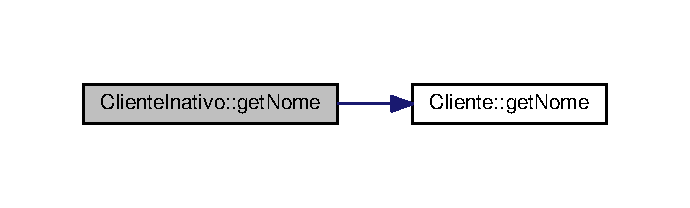
\includegraphics[width=331pt]{classClienteInativo_a0d29faf815a74d59a7f3e4028d5aad2a_cgraph}
\end{center}
\end{figure}




Here is the caller graph for this function\+:\nopagebreak
\begin{figure}[H]
\begin{center}
\leavevmode
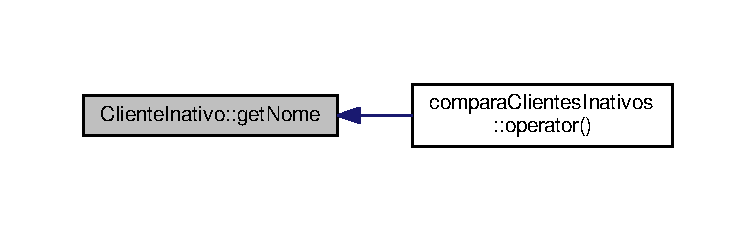
\includegraphics[width=350pt]{classClienteInativo_a0d29faf815a74d59a7f3e4028d5aad2a_icgraph}
\end{center}
\end{figure}


\index{Cliente\+Inativo@{Cliente\+Inativo}!set\+Morada@{set\+Morada}}
\index{set\+Morada@{set\+Morada}!Cliente\+Inativo@{Cliente\+Inativo}}
\subsubsection[{\texorpdfstring{set\+Morada(std\+::string nova\+Morada)}{setMorada(std::string novaMorada)}}]{\setlength{\rightskip}{0pt plus 5cm}void Cliente\+Inativo\+::set\+Morada (
\begin{DoxyParamCaption}
\item[{std\+::string}]{nova\+Morada}
\end{DoxyParamCaption}
)}\hypertarget{classClienteInativo_aea3df2299f33ea2f4e22f406ba73d5b2}{}\label{classClienteInativo_aea3df2299f33ea2f4e22f406ba73d5b2}


Sets the address. 


\begin{DoxyParams}[1]{Parameters}
\mbox{\tt in}  & {\em nova\+Morada} & The new address \\
\hline
\end{DoxyParams}

\begin{DoxyCode}
491                                                \{
492     this->\hyperlink{classClienteInativo_aea3df2299f33ea2f4e22f406ba73d5b2}{setMorada}(novaMorada);
493 \}
\end{DoxyCode}


The documentation for this class was generated from the following files\+:\begin{DoxyCompactItemize}
\item 
/home/joao/\+Documentos/\+Projetos/\+Porto-\/rivers-\/cruise-\/manager/src/\hyperlink{cruise_8h}{cruise.\+h}\item 
/home/joao/\+Documentos/\+Projetos/\+Porto-\/rivers-\/cruise-\/manager/src/\hyperlink{cruise_8cpp}{cruise.\+cpp}\end{DoxyCompactItemize}

\hypertarget{classClienteRegistado}{}\section{Cliente\+Registado Class Reference}
\label{classClienteRegistado}\index{Cliente\+Registado@{Cliente\+Registado}}


{\ttfamily \#include $<$cruise.\+h$>$}

Inheritance diagram for Cliente\+Registado\+:\begin{figure}[H]
\begin{center}
\leavevmode
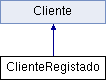
\includegraphics[height=2.000000cm]{classClienteRegistado}
\end{center}
\end{figure}
\subsection*{Public Member Functions}
\begin{DoxyCompactItemize}
\item 
\hyperlink{classClienteRegistado_a27df6b812a22aa40e43968b4cfc7eec6}{Cliente\+Registado} (std\+::string \hyperlink{classCliente_aaa79b0a26f7d5d007fe4ae9696564ca5}{nome}, unsigned int \hyperlink{classClienteRegistado_a137b6b72d824b38eabcfcb78671dd495}{pontos}=0)
\item 
unsigned int \hyperlink{classClienteRegistado_a0118e31f16e4dce542f5e1d124d26c61}{get\+Pontos} ()
\item 
void \hyperlink{classClienteRegistado_a0148a97dd713addd6a932f282e076ba3}{add\+Pontos} (unsigned int \hyperlink{classClienteRegistado_a137b6b72d824b38eabcfcb78671dd495}{pontos})
\item 
bool \hyperlink{classClienteRegistado_a3dade20423acb0e84c9fbe30c75f0e3e}{is\+Registado} ()
\end{DoxyCompactItemize}
\subsection*{Private Attributes}
\begin{DoxyCompactItemize}
\item 
unsigned int \hyperlink{classClienteRegistado_a137b6b72d824b38eabcfcb78671dd495}{pontos}
\end{DoxyCompactItemize}
\subsection*{Additional Inherited Members}


\subsection{Constructor \& Destructor Documentation}
\mbox{\Hypertarget{classClienteRegistado_a27df6b812a22aa40e43968b4cfc7eec6}\label{classClienteRegistado_a27df6b812a22aa40e43968b4cfc7eec6}} 
\index{Cliente\+Registado@{Cliente\+Registado}!Cliente\+Registado@{Cliente\+Registado}}
\index{Cliente\+Registado@{Cliente\+Registado}!Cliente\+Registado@{Cliente\+Registado}}
\subsubsection{\texorpdfstring{Cliente\+Registado()}{ClienteRegistado()}}
{\footnotesize\ttfamily Cliente\+Registado\+::\+Cliente\+Registado (\begin{DoxyParamCaption}\item[{std\+::string}]{nome,  }\item[{unsigned int}]{pontos = {\ttfamily 0} }\end{DoxyParamCaption})}



\subsection{Member Function Documentation}
\mbox{\Hypertarget{classClienteRegistado_a0148a97dd713addd6a932f282e076ba3}\label{classClienteRegistado_a0148a97dd713addd6a932f282e076ba3}} 
\index{Cliente\+Registado@{Cliente\+Registado}!add\+Pontos@{add\+Pontos}}
\index{add\+Pontos@{add\+Pontos}!Cliente\+Registado@{Cliente\+Registado}}
\subsubsection{\texorpdfstring{add\+Pontos()}{addPontos()}}
{\footnotesize\ttfamily void Cliente\+Registado\+::add\+Pontos (\begin{DoxyParamCaption}\item[{unsigned int}]{pontos }\end{DoxyParamCaption})}

\mbox{\Hypertarget{classClienteRegistado_a0118e31f16e4dce542f5e1d124d26c61}\label{classClienteRegistado_a0118e31f16e4dce542f5e1d124d26c61}} 
\index{Cliente\+Registado@{Cliente\+Registado}!get\+Pontos@{get\+Pontos}}
\index{get\+Pontos@{get\+Pontos}!Cliente\+Registado@{Cliente\+Registado}}
\subsubsection{\texorpdfstring{get\+Pontos()}{getPontos()}}
{\footnotesize\ttfamily unsigned int Cliente\+Registado\+::get\+Pontos (\begin{DoxyParamCaption}{ }\end{DoxyParamCaption})\hspace{0.3cm}{\ttfamily [inline]}, {\ttfamily [virtual]}}



Reimplemented from \hyperlink{classCliente_a4bcd51f0d9a0bfe7d9d47074ac4e65de}{Cliente}.

\mbox{\Hypertarget{classClienteRegistado_a3dade20423acb0e84c9fbe30c75f0e3e}\label{classClienteRegistado_a3dade20423acb0e84c9fbe30c75f0e3e}} 
\index{Cliente\+Registado@{Cliente\+Registado}!is\+Registado@{is\+Registado}}
\index{is\+Registado@{is\+Registado}!Cliente\+Registado@{Cliente\+Registado}}
\subsubsection{\texorpdfstring{is\+Registado()}{isRegistado()}}
{\footnotesize\ttfamily bool Cliente\+Registado\+::is\+Registado (\begin{DoxyParamCaption}{ }\end{DoxyParamCaption})\hspace{0.3cm}{\ttfamily [inline]}, {\ttfamily [virtual]}}



Reimplemented from \hyperlink{classCliente_acb60d8bf04134b986ae56a79db8beaaf}{Cliente}.



\subsection{Member Data Documentation}
\mbox{\Hypertarget{classClienteRegistado_a137b6b72d824b38eabcfcb78671dd495}\label{classClienteRegistado_a137b6b72d824b38eabcfcb78671dd495}} 
\index{Cliente\+Registado@{Cliente\+Registado}!pontos@{pontos}}
\index{pontos@{pontos}!Cliente\+Registado@{Cliente\+Registado}}
\subsubsection{\texorpdfstring{pontos}{pontos}}
{\footnotesize\ttfamily unsigned int Cliente\+Registado\+::pontos\hspace{0.3cm}{\ttfamily [private]}}



The documentation for this class was generated from the following files\+:\begin{DoxyCompactItemize}
\item 
/home/joao/\+Documentos/\+Projectos/\+Porto-\/rivers-\/cruise-\/manager/src/\hyperlink{cruise_8h}{cruise.\+h}\item 
/home/joao/\+Documentos/\+Projectos/\+Porto-\/rivers-\/cruise-\/manager/src/\hyperlink{cruise_8cpp}{cruise.\+cpp}\end{DoxyCompactItemize}

\hypertarget{structcomparaClientesInativos}{}\section{compara\+Clientes\+Inativos Struct Reference}
\label{structcomparaClientesInativos}\index{compara\+Clientes\+Inativos@{compara\+Clientes\+Inativos}}


Comparison criteria in the hash table.  




{\ttfamily \#include $<$cruise.\+h$>$}

\subsection*{Public Member Functions}
\begin{DoxyCompactItemize}
\item 
int \hyperlink{structcomparaClientesInativos_a8f260b392f56aa5f619fcd2c3a871fb4}{operator()} (const \hyperlink{classClienteInativo}{Cliente\+Inativo} \&c) const 
\item 
bool \hyperlink{structcomparaClientesInativos_aae4b963001183c30c0aab8b597e3c61d}{operator()} (const \hyperlink{classClienteInativo}{Cliente\+Inativo} \&c1, const \hyperlink{classClienteInativo}{Cliente\+Inativo} \&c2) const 
\end{DoxyCompactItemize}


\subsection{Detailed Description}
Comparison criteria in the hash table. 

\subsection{Member Function Documentation}
\index{compara\+Clientes\+Inativos@{compara\+Clientes\+Inativos}!operator()@{operator()}}
\index{operator()@{operator()}!compara\+Clientes\+Inativos@{compara\+Clientes\+Inativos}}
\subsubsection[{\texorpdfstring{operator()(const Cliente\+Inativo \&c) const }{operator()(const ClienteInativo &c) const }}]{\setlength{\rightskip}{0pt plus 5cm}int compara\+Clientes\+Inativos\+::operator() (
\begin{DoxyParamCaption}
\item[{const {\bf Cliente\+Inativo} \&}]{c}
\end{DoxyParamCaption}
) const\hspace{0.3cm}{\ttfamily [inline]}}\hypertarget{structcomparaClientesInativos_a8f260b392f56aa5f619fcd2c3a871fb4}{}\label{structcomparaClientesInativos_a8f260b392f56aa5f619fcd2c3a871fb4}

\begin{DoxyCode}
579                                                     \{
580         \textcolor{keywordflow}{return} 0;
581     \}
\end{DoxyCode}
\index{compara\+Clientes\+Inativos@{compara\+Clientes\+Inativos}!operator()@{operator()}}
\index{operator()@{operator()}!compara\+Clientes\+Inativos@{compara\+Clientes\+Inativos}}
\subsubsection[{\texorpdfstring{operator()(const Cliente\+Inativo \&c1, const Cliente\+Inativo \&c2) const }{operator()(const ClienteInativo &c1, const ClienteInativo &c2) const }}]{\setlength{\rightskip}{0pt plus 5cm}bool compara\+Clientes\+Inativos\+::operator() (
\begin{DoxyParamCaption}
\item[{const {\bf Cliente\+Inativo} \&}]{c1, }
\item[{const {\bf Cliente\+Inativo} \&}]{c2}
\end{DoxyParamCaption}
) const\hspace{0.3cm}{\ttfamily [inline]}}\hypertarget{structcomparaClientesInativos_aae4b963001183c30c0aab8b597e3c61d}{}\label{structcomparaClientesInativos_aae4b963001183c30c0aab8b597e3c61d}

\begin{DoxyCode}
582                                                                                  \{
583         \textcolor{keywordflow}{return} c1.\hyperlink{classClienteInativo_a0d29faf815a74d59a7f3e4028d5aad2a}{getNome}() < c2.\hyperlink{classClienteInativo_a0d29faf815a74d59a7f3e4028d5aad2a}{getNome}();
584     \}
\end{DoxyCode}


Here is the call graph for this function\+:
\nopagebreak
\begin{figure}[H]
\begin{center}
\leavevmode
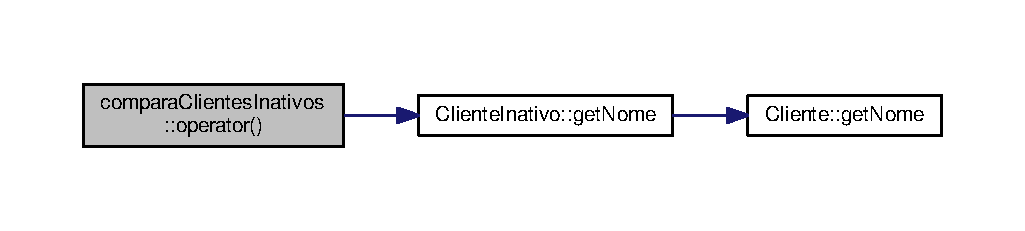
\includegraphics[width=350pt]{structcomparaClientesInativos_aae4b963001183c30c0aab8b597e3c61d_cgraph}
\end{center}
\end{figure}




The documentation for this struct was generated from the following file\+:\begin{DoxyCompactItemize}
\item 
/home/joao/\+Documentos/\+Projetos/\+Porto-\/rivers-\/cruise-\/manager/src/\hyperlink{cruise_8h}{cruise.\+h}\end{DoxyCompactItemize}

\hypertarget{structcomparaOfertas}{}\section{compara\+Ofertas Struct Reference}
\label{structcomparaOfertas}\index{compara\+Ofertas@{compara\+Ofertas}}


Comparison criteria in the prioritie queue.  




{\ttfamily \#include $<$cruise.\+h$>$}

\subsection*{Public Member Functions}
\begin{DoxyCompactItemize}
\item 
bool \hyperlink{structcomparaOfertas_a8b792bc79e9870004caa3e95826a0f1f}{operator()} (\hyperlink{classOferta}{Oferta} oferta1, \hyperlink{classOferta}{Oferta} oferta2) const 
\end{DoxyCompactItemize}


\subsection{Detailed Description}
Comparison criteria in the prioritie queue. 

\subsection{Member Function Documentation}
\index{compara\+Ofertas@{compara\+Ofertas}!operator()@{operator()}}
\index{operator()@{operator()}!compara\+Ofertas@{compara\+Ofertas}}
\subsubsection[{\texorpdfstring{operator()(\+Oferta oferta1, Oferta oferta2) const }{operator()(Oferta oferta1, Oferta oferta2) const }}]{\setlength{\rightskip}{0pt plus 5cm}bool compara\+Ofertas\+::operator() (
\begin{DoxyParamCaption}
\item[{{\bf Oferta}}]{oferta1, }
\item[{{\bf Oferta}}]{oferta2}
\end{DoxyParamCaption}
) const\hspace{0.3cm}{\ttfamily [inline]}}\hypertarget{structcomparaOfertas_a8b792bc79e9870004caa3e95826a0f1f}{}\label{structcomparaOfertas_a8b792bc79e9870004caa3e95826a0f1f}

\begin{DoxyCode}
569                                                            \{
570         \textcolor{keywordflow}{return} oferta1.\hyperlink{classOferta_a1caf2c681c14c9fbd04312b35f99b64c}{getUltimaReserva}() < oferta2.
      \hyperlink{classOferta_a1caf2c681c14c9fbd04312b35f99b64c}{getUltimaReserva}();
571     \}
\end{DoxyCode}


Here is the call graph for this function\+:\nopagebreak
\begin{figure}[H]
\begin{center}
\leavevmode
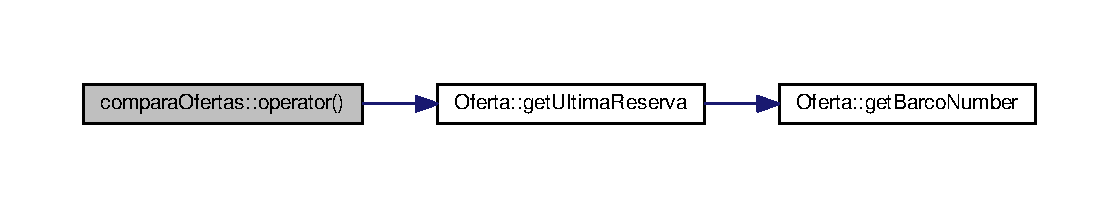
\includegraphics[width=350pt]{structcomparaOfertas_a8b792bc79e9870004caa3e95826a0f1f_cgraph}
\end{center}
\end{figure}




The documentation for this struct was generated from the following file\+:\begin{DoxyCompactItemize}
\item 
/home/joao/\+Documentos/\+Projetos/\+Porto-\/rivers-\/cruise-\/manager/src/\hyperlink{cruise_8h}{cruise.\+h}\end{DoxyCompactItemize}

\hypertarget{classEmpresa}{}\section{Empresa Class Reference}
\label{classEmpresa}\index{Empresa@{Empresa}}


Class for empresa.  




{\ttfamily \#include $<$cruise.\+h$>$}

\subsection*{Public Member Functions}
\begin{DoxyCompactItemize}
\item 
\hyperlink{classEmpresa_aff124b958356c479ab50ddf4cf302193}{Empresa} ()
\begin{DoxyCompactList}\small\item\em Construct \hyperlink{classEmpresa}{Empresa} object. \end{DoxyCompactList}\item 
\hyperlink{classEmpresa}{Empresa} \& \hyperlink{classEmpresa_a0c858479d6e92094adbb2fc085039376}{add\+Fornecedores} (\hyperlink{classFornecedor}{Fornecedor} \&f)
\begin{DoxyCompactList}\small\item\em Adds suppliers. \end{DoxyCompactList}\item 
\hyperlink{classEmpresa}{Empresa} \& \hyperlink{classEmpresa_a57597ec4154f274686bc648ccf5d2a59}{add\+Clientes} (\hyperlink{classCliente}{Cliente} \&c)
\begin{DoxyCompactList}\small\item\em Adds a clients. \end{DoxyCompactList}\item 
\hyperlink{classEmpresa}{Empresa} \& \hyperlink{classEmpresa_a42a1671b234ab8380cfb2ed33517edb2}{add\+Reservas} (\hyperlink{classReserva}{Reserva} \&r)
\begin{DoxyCompactList}\small\item\em Adds a reservation. \end{DoxyCompactList}\item 
\hyperlink{classEmpresa}{Empresa} \& \hyperlink{classEmpresa_a89c034ba48b716dfe61724e38eb0afbb}{add\+Faturas} (\hyperlink{classFatura}{Fatura} \&r)
\begin{DoxyCompactList}\small\item\em Adds a bill. \end{DoxyCompactList}\item 
\hyperlink{classEmpresa}{Empresa} \& \hyperlink{classEmpresa_ab8b7dda77caceec58e464c16b7e45f7c}{delete\+Fornecedores} (std\+::string name)
\begin{DoxyCompactList}\small\item\em removes a supplier \end{DoxyCompactList}\item 
\hyperlink{classEmpresa}{Empresa} \& \hyperlink{classEmpresa_a52b9f4d94c2a05704d74854ed4dd1590}{delete\+Clientes} (std\+::string name)
\begin{DoxyCompactList}\small\item\em removes a Client \end{DoxyCompactList}\item 
\hyperlink{classEmpresa}{Empresa} \& \hyperlink{classEmpresa_a079c008b006f56faac3c1016fe770e8c}{delete\+Reservas} (std\+::string name)
\begin{DoxyCompactList}\small\item\em removes a Reservation \end{DoxyCompactList}\item 
void \hyperlink{classEmpresa_ad79f7196a8ce7256771cbd7b9542155c}{titulo} ()
\begin{DoxyCompactList}\small\item\em displays the main title of the company \end{DoxyCompactList}\item 
void \hyperlink{classEmpresa_ad77cdd5a6cbe2beb2078aa6bec2cfe28}{menu\+Inicial} ()
\begin{DoxyCompactList}\small\item\em displays the first menu \end{DoxyCompactList}\item 
void \hyperlink{classEmpresa_a544832c17fe7d592ae1d01bdc144059e}{menu\+Tipode\+Utilizador} ()
\begin{DoxyCompactList}\small\item\em Displays a menu that guides the user to all the sub-\/menus. \end{DoxyCompactList}\item 
void \hyperlink{classEmpresa_a2e8e13ecd162403da0118ceccdccbbcb}{menu\+Cliente} ()
\begin{DoxyCompactList}\small\item\em displays the Client Menu \end{DoxyCompactList}\item 
void \hyperlink{classEmpresa_a372599c8aee20690517cc3ae6c8e1ca7}{adiciona\+Cliente\+Normal} ()
\begin{DoxyCompactList}\small\item\em displays the interface to add Clients \end{DoxyCompactList}\item 
void \hyperlink{classEmpresa_a430c00a63ef70338de3b4b7c096ea194}{adiciona\+Cliente\+Registado} ()
\begin{DoxyCompactList}\small\item\em displays the interface to add Registred Clients \end{DoxyCompactList}\item 
void \hyperlink{classEmpresa_aba4af6a945948ac66e771a416cfc2a2a}{adiciona\+Cliente} ()
\begin{DoxyCompactList}\small\item\em adds Clients \end{DoxyCompactList}\item 
void \hyperlink{classEmpresa_a9b938f2436e95e68afce6cc04f2100bc}{modifica\+Cliente} ()
\begin{DoxyCompactList}\small\item\em Modifies a cliente. \end{DoxyCompactList}\item 
void \hyperlink{classEmpresa_ab9af9446d6d2c206b4b3e18e1bcb6475}{remove\+Cliente} ()
\begin{DoxyCompactList}\small\item\em Removes a cliente. \end{DoxyCompactList}\item 
void \hyperlink{classEmpresa_adb9d8d4aa55f253fc534e220ca4a87ac}{menu\+Fornecedor} ()
\begin{DoxyCompactList}\small\item\em displays the Supplier Menu \end{DoxyCompactList}\item 
void \hyperlink{classEmpresa_af20261a3f95a5dd0c4a5a796d9a3d442}{adiciona\+Fornecedor} ()
\begin{DoxyCompactList}\small\item\em displays the interface to add suppliers \end{DoxyCompactList}\item 
void \hyperlink{classEmpresa_aa0470e1fd4f41615a230fc8048b8b321}{modifica\+Fornecedor} ()
\begin{DoxyCompactList}\small\item\em Modifies a supplier. \end{DoxyCompactList}\item 
void \hyperlink{classEmpresa_a9aa7b7e699971eb2e28f0db99c6500c4}{remove\+Fornecedor} ()
\begin{DoxyCompactList}\small\item\em Removes a supplier. \end{DoxyCompactList}\item 
void \hyperlink{classEmpresa_a0d362cb7362b859ccf99b9603de6b603}{menu\+Reservas} ()
\begin{DoxyCompactList}\small\item\em displays the Reservations Menu \end{DoxyCompactList}\item 
void \hyperlink{classEmpresa_a42953bdbb2fb39173ad6f38892fc122b}{adiciona\+Reserva} ()
\begin{DoxyCompactList}\small\item\em displays the interface to add reservations \end{DoxyCompactList}\item 
void \hyperlink{classEmpresa_ae74f80c120a14f0591d04fe7603e6905}{modifica\+Reserva} ()
\begin{DoxyCompactList}\small\item\em displays the interface to modify reservations \end{DoxyCompactList}\item 
void \hyperlink{classEmpresa_aa0b169a112c75b6fd1bc80128720282e}{cancela\+Reservas} ()
\begin{DoxyCompactList}\small\item\em displays the interface to cancel reservations \end{DoxyCompactList}\item 
void \hyperlink{classEmpresa_a3e0ee0b5d92f0cd655a26095229849f1}{remove\+Reservas} ()
\begin{DoxyCompactList}\small\item\em displays the interface to remove reservations \end{DoxyCompactList}\item 
void \hyperlink{classEmpresa_a58d040d3983d55414d5c6fac5ac3b6c5}{menu\+Faturas} ()
\begin{DoxyCompactList}\small\item\em displays the interface related to bills \end{DoxyCompactList}\item 
void \hyperlink{classEmpresa_ab1950b5b5e9fca80823b5d01c6c1de6f}{lista\+Faturas} ()
\begin{DoxyCompactList}\small\item\em Lists all the bills. \end{DoxyCompactList}\item 
void \hyperlink{classEmpresa_a3cab1a61ff84c5b20ac2faa6251e25ed}{menu\+Ofertas} ()
\begin{DoxyCompactList}\small\item\em displays the offers Menu \end{DoxyCompactList}\item 
void \hyperlink{classEmpresa_ae244a8ae3afb85eb5e9e5febce8b8728}{adiciona\+Oferta} ()
\begin{DoxyCompactList}\small\item\em displays the interface to adds offers \end{DoxyCompactList}\item 
void \hyperlink{classEmpresa_ac8948065c65d5c02cb30103118f502d4}{modifica\+Oferta} ()
\begin{DoxyCompactList}\small\item\em displays the interface to modify offers \end{DoxyCompactList}\item 
void \hyperlink{classEmpresa_a5b5c42d733ccee37f932db5db8aec243}{remove\+Oferta} ()
\begin{DoxyCompactList}\small\item\em displays the interface to remove offers \end{DoxyCompactList}\item 
void \hyperlink{classEmpresa_a5ca8821d938f11f29558ae90913de528}{add\+Ofertas\+Queue} ()
\begin{DoxyCompactList}\small\item\em displays all the information about the Offerts in priority order \end{DoxyCompactList}\item 
void \hyperlink{classEmpresa_acd458614a3cca3f432b54212a2e72584}{display\+Ofertasem\+Ordem} ()
\begin{DoxyCompactList}\small\item\em displays all the information about the Offerts without priority order \end{DoxyCompactList}\item 
void \hyperlink{classEmpresa_a28e04d59daa7206bec6055249ce17410}{display\+Clientes} ()
\begin{DoxyCompactList}\small\item\em displays all the information about the Clients \end{DoxyCompactList}\item 
void \hyperlink{classEmpresa_a55c3756c01b45b41ad03f4e4f3e4dcac}{display\+Fornecedores} ()
\begin{DoxyCompactList}\small\item\em displays all the information about the suppliers; \end{DoxyCompactList}\item 
void \hyperlink{classEmpresa_aa47e9a64800a41180b7f374b73a1f32b}{display\+Fornecedorescom\+Ofertas} ()
\begin{DoxyCompactList}\small\item\em displays all the information about the suppliers all their respective offers \end{DoxyCompactList}\item 
void \hyperlink{classEmpresa_a8c89e6053eaccf0e1938a4f2ab0bfdc4}{display\+Reservas} ()
\begin{DoxyCompactList}\small\item\em displays all the information about the reservations \end{DoxyCompactList}\item 
const std\+::vector$<$ \hyperlink{classFornecedor}{Fornecedor} $\ast$ $>$ \& \hyperlink{classEmpresa_aaf131a375aa70819205744328a4dbc07}{get\+Fornecedores} ()
\begin{DoxyCompactList}\small\item\em Gets the suppliers. \end{DoxyCompactList}\item 
const std\+::vector$<$ \hyperlink{classCliente}{Cliente} $\ast$ $>$ \& \hyperlink{classEmpresa_a472beae89ee1187e1ec3f70e9d4a99ef}{get\+Clientes} ()
\begin{DoxyCompactList}\small\item\em Gets the clients. \end{DoxyCompactList}\item 
void \hyperlink{classEmpresa_afbde694da902870437443de43dae8071}{save} ()
\begin{DoxyCompactList}\small\item\em stores in a text file all the information generated by the program execution \end{DoxyCompactList}\item 
void \hyperlink{classEmpresa_a3445c3c507b4f45d1d7831908ff4cdf1}{load} ()
\begin{DoxyCompactList}\small\item\em loads the information generated in previous executions \end{DoxyCompactList}\item 
void \hyperlink{classEmpresa_aa7424cde3bdf1b1921967bc176d0ab50}{sort} ()
\begin{DoxyCompactList}\small\item\em sorts the vectors of the class \end{DoxyCompactList}\item 
\hyperlink{classEmpresa}{Empresa} \& \hyperlink{classEmpresa_a4c8205b2c4aad43f46172966aaed30b7}{desativa\+Cliente} (\hyperlink{classCliente}{Cliente} $\ast$c)
\begin{DoxyCompactList}\small\item\em Makes a client inactive. \end{DoxyCompactList}\item 
\hyperlink{classEmpresa}{Empresa} \& \hyperlink{classEmpresa_aea372dbf680408d9fb32341c03b3e5ad}{atualiza\+Inatividade} ()
\begin{DoxyCompactList}\small\item\em Updates which clients are inactive. \end{DoxyCompactList}\item 
\hyperlink{classEmpresa}{Empresa} \& \hyperlink{classEmpresa_a64b9a495ca3a80380646814557be4924}{reativa\+Cliente} (\hyperlink{classCliente}{Cliente} $\ast$c)
\begin{DoxyCompactList}\small\item\em Makes a client active again. \end{DoxyCompactList}\item 
void \hyperlink{classEmpresa_ac7ea4de24979f6623ffe8fbd3d0eeb24}{display\+Clientes\+Inativos} ()
\begin{DoxyCompactList}\small\item\em Lists all the inactive clients. \end{DoxyCompactList}\item 
void \hyperlink{classEmpresa_a259bb6b172011429c6e24feb0285e66b}{display\+Todas\+As\+Reservasde\+Um\+Cliente} ()
\begin{DoxyCompactList}\small\item\em Lists all the reservations made by one client. \end{DoxyCompactList}\item 
void \hyperlink{classEmpresa_af197726a3dc20739aac877ac4c090f6e}{display\+Todas\+As\+Reservasde\+Um\+Fornecedor} ()
\begin{DoxyCompactList}\small\item\em Lists all the reservations with offers of one supplier. \end{DoxyCompactList}\item 
void \hyperlink{classEmpresa_a73543b5ca1d9dd8e99e75d9167839471}{display\+Todas\+As\+Ofertasde\+Um\+Fornecedor} ()
\begin{DoxyCompactList}\small\item\em Lists all the offers of one Supplier. \end{DoxyCompactList}\item 
void \hyperlink{classEmpresa_a641c2eb827b39ab79919187645ff71a9}{display\+Todos\+Os\+Clientesdeuma\+Oferta} ()
\begin{DoxyCompactList}\small\item\em Lists all the clients that reserved a certain offer. \end{DoxyCompactList}\item 
void \hyperlink{classEmpresa_a46a4898b8ae8e09bdf656b25b8ffe99d}{aplica\+Desconto} ()
\begin{DoxyCompactList}\small\item\em Applies discount. \end{DoxyCompactList}\end{DoxyCompactItemize}


\subsection{Detailed Description}
Class for empresa. 

\subsection{Constructor \& Destructor Documentation}
\index{Empresa@{Empresa}!Empresa@{Empresa}}
\index{Empresa@{Empresa}!Empresa@{Empresa}}
\subsubsection[{\texorpdfstring{Empresa()}{Empresa()}}]{\setlength{\rightskip}{0pt plus 5cm}Empresa\+::\+Empresa (
\begin{DoxyParamCaption}
{}
\end{DoxyParamCaption}
)}\hypertarget{classEmpresa_aff124b958356c479ab50ddf4cf302193}{}\label{classEmpresa_aff124b958356c479ab50ddf4cf302193}


Construct \hyperlink{classEmpresa}{Empresa} object. 

Metodos da classe \hyperlink{classEmpresa}{Empresa} ////.

Constructs object of type \hyperlink{classEmpresa}{Empresa} 
\begin{DoxyCode}
22                 : \_faturas(\hyperlink{classFatura}{Fatura}(NULL))\{
23     this->\hyperlink{classEmpresa_a3445c3c507b4f45d1d7831908ff4cdf1}{load}();
24     \hyperlink{classEmpresa_aea372dbf680408d9fb32341c03b3e5ad}{atualizaInatividade}();
25     \hyperlink{classEmpresa_a5ca8821d938f11f29558ae90913de528}{addOfertasQueue}();
26     this->\hyperlink{classEmpresa_ad77cdd5a6cbe2beb2078aa6bec2cfe28}{menuInicial}();
27     this->\hyperlink{classEmpresa_afbde694da902870437443de43dae8071}{save}();
28 \}
\end{DoxyCode}


Here is the call graph for this function\+:
\nopagebreak
\begin{figure}[H]
\begin{center}
\leavevmode
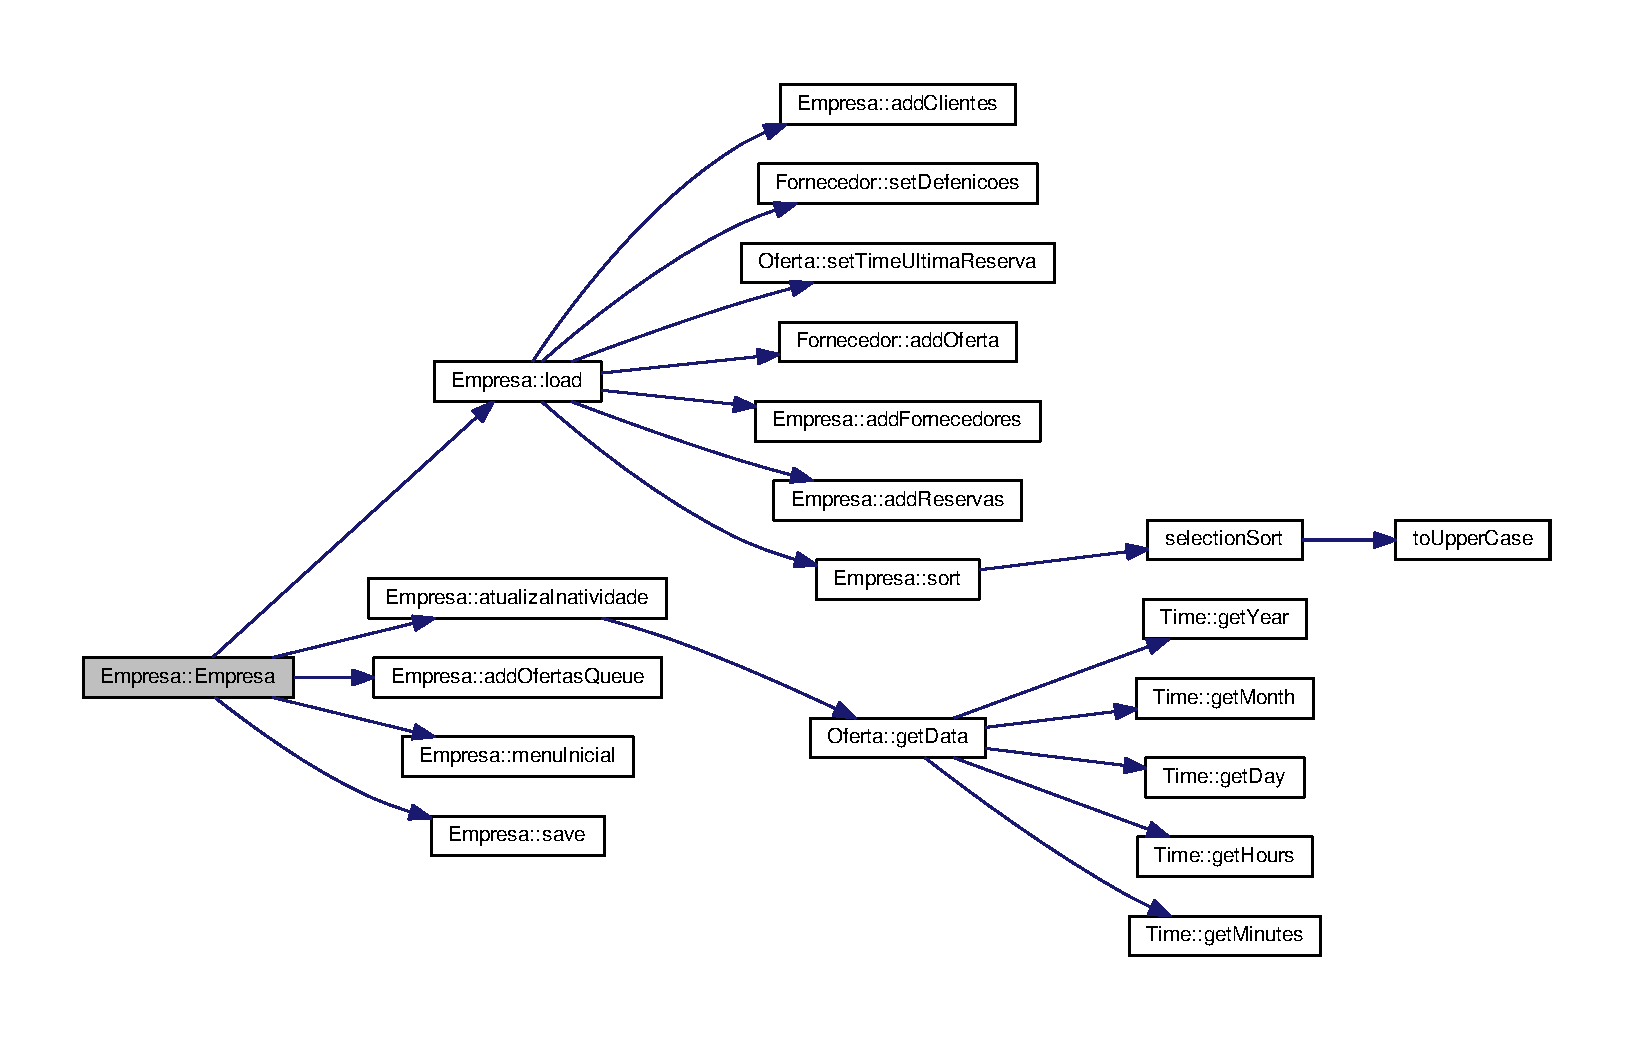
\includegraphics[width=350pt]{classEmpresa_aff124b958356c479ab50ddf4cf302193_cgraph}
\end{center}
\end{figure}




\subsection{Member Function Documentation}
\index{Empresa@{Empresa}!add\+Clientes@{add\+Clientes}}
\index{add\+Clientes@{add\+Clientes}!Empresa@{Empresa}}
\subsubsection[{\texorpdfstring{add\+Clientes(\+Cliente \&c)}{addClientes(Cliente &c)}}]{\setlength{\rightskip}{0pt plus 5cm}{\bf Empresa} \& Empresa\+::add\+Clientes (
\begin{DoxyParamCaption}
\item[{{\bf Cliente} \&}]{c}
\end{DoxyParamCaption}
)}\hypertarget{classEmpresa_a57597ec4154f274686bc648ccf5d2a59}{}\label{classEmpresa_a57597ec4154f274686bc648ccf5d2a59}


Adds a clients. 


\begin{DoxyParams}{Parameters}
{\em c} & Client\\
\hline
\end{DoxyParams}
\begin{DoxyReturn}{Returns}
the modified company 
\end{DoxyReturn}

\begin{DoxyCode}
43                                         \{
44     this->\_clientes.push\_back(&c);
45     \textcolor{keywordflow}{return} *\textcolor{keyword}{this};
46 \}
\end{DoxyCode}


Here is the caller graph for this function\+:\nopagebreak
\begin{figure}[H]
\begin{center}
\leavevmode
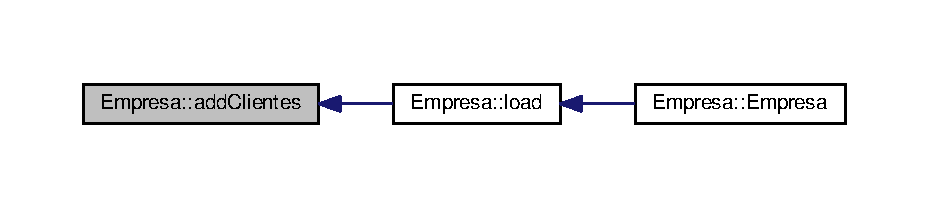
\includegraphics[width=350pt]{classEmpresa_a57597ec4154f274686bc648ccf5d2a59_icgraph}
\end{center}
\end{figure}


\index{Empresa@{Empresa}!add\+Faturas@{add\+Faturas}}
\index{add\+Faturas@{add\+Faturas}!Empresa@{Empresa}}
\subsubsection[{\texorpdfstring{add\+Faturas(\+Fatura \&r)}{addFaturas(Fatura &r)}}]{\setlength{\rightskip}{0pt plus 5cm}{\bf Empresa} \& Empresa\+::add\+Faturas (
\begin{DoxyParamCaption}
\item[{{\bf Fatura} \&}]{r}
\end{DoxyParamCaption}
)}\hypertarget{classEmpresa_a89c034ba48b716dfe61724e38eb0afbb}{}\label{classEmpresa_a89c034ba48b716dfe61724e38eb0afbb}


Adds a bill. 


\begin{DoxyParams}{Parameters}
{\em r} & the bill\\
\hline
\end{DoxyParams}
\begin{DoxyReturn}{Returns}
the modified company 
\end{DoxyReturn}

\begin{DoxyCode}
646                                       \{
647     this->\_faturas.\hyperlink{classBST_a2b117df6521c7d61dac75ff2c938bae7}{insert}(r);
648     \textcolor{keywordflow}{return} *\textcolor{keyword}{this};
649 \}
\end{DoxyCode}
\index{Empresa@{Empresa}!add\+Fornecedores@{add\+Fornecedores}}
\index{add\+Fornecedores@{add\+Fornecedores}!Empresa@{Empresa}}
\subsubsection[{\texorpdfstring{add\+Fornecedores(\+Fornecedor \&f)}{addFornecedores(Fornecedor &f)}}]{\setlength{\rightskip}{0pt plus 5cm}{\bf Empresa} \& Empresa\+::add\+Fornecedores (
\begin{DoxyParamCaption}
\item[{{\bf Fornecedor} \&}]{f}
\end{DoxyParamCaption}
)}\hypertarget{classEmpresa_a0c858479d6e92094adbb2fc085039376}{}\label{classEmpresa_a0c858479d6e92094adbb2fc085039376}


Adds suppliers. 


\begin{DoxyParams}{Parameters}
{\em f} & \hyperlink{classFornecedor}{Fornecedor}\\
\hline
\end{DoxyParams}
\begin{DoxyReturn}{Returns}
the modified \hyperlink{classEmpresa}{Empresa} 
\end{DoxyReturn}

\begin{DoxyCode}
38                                                \{
39     this->\_fornecedores.push\_back(&f);
40     \textcolor{keywordflow}{return} *\textcolor{keyword}{this};
41 \}
\end{DoxyCode}


Here is the caller graph for this function\+:\nopagebreak
\begin{figure}[H]
\begin{center}
\leavevmode
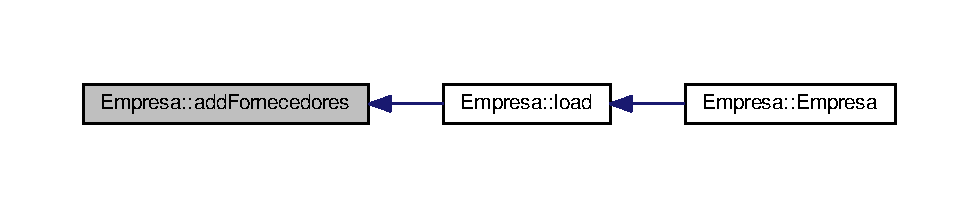
\includegraphics[width=350pt]{classEmpresa_a0c858479d6e92094adbb2fc085039376_icgraph}
\end{center}
\end{figure}


\index{Empresa@{Empresa}!add\+Ofertas\+Queue@{add\+Ofertas\+Queue}}
\index{add\+Ofertas\+Queue@{add\+Ofertas\+Queue}!Empresa@{Empresa}}
\subsubsection[{\texorpdfstring{add\+Ofertas\+Queue()}{addOfertasQueue()}}]{\setlength{\rightskip}{0pt plus 5cm}void Empresa\+::add\+Ofertas\+Queue (
\begin{DoxyParamCaption}
{}
\end{DoxyParamCaption}
)}\hypertarget{classEmpresa_a5ca8821d938f11f29558ae90913de528}{}\label{classEmpresa_a5ca8821d938f11f29558ae90913de528}


displays all the information about the Offerts in priority order 


\begin{DoxyCode}
552 \{
553     \textcolor{keywordflow}{while} (!queueOfertasOrdenadas.empty()) \{
554         queueOfertasOrdenadas.pop();
555     \}
556 
557     \textcolor{keywordflow}{for} (\textcolor{keywordtype}{unsigned} \textcolor{keywordtype}{int} i = 0; i < \_fornecedores.size(); i++)
558     \{
559         \textcolor{keywordflow}{for} (\textcolor{keywordtype}{unsigned} \textcolor{keywordtype}{int} j = 0; j < \_fornecedores[i]->getOfertas().size(); j++)
560         \{
561             queueOfertasOrdenadas.push(\_fornecedores[i]->getOfertas()[j]);
562         \}
563     \}
564 \}
\end{DoxyCode}


Here is the caller graph for this function\+:\nopagebreak
\begin{figure}[H]
\begin{center}
\leavevmode
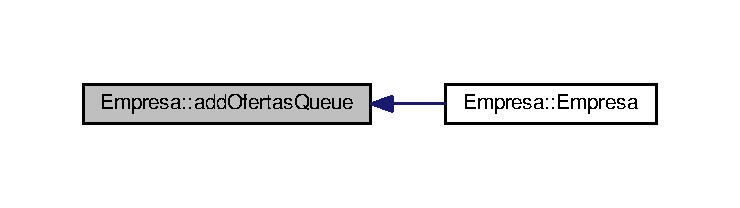
\includegraphics[width=350pt]{classEmpresa_a5ca8821d938f11f29558ae90913de528_icgraph}
\end{center}
\end{figure}


\index{Empresa@{Empresa}!add\+Reservas@{add\+Reservas}}
\index{add\+Reservas@{add\+Reservas}!Empresa@{Empresa}}
\subsubsection[{\texorpdfstring{add\+Reservas(\+Reserva \&r)}{addReservas(Reserva &r)}}]{\setlength{\rightskip}{0pt plus 5cm}{\bf Empresa} \& Empresa\+::add\+Reservas (
\begin{DoxyParamCaption}
\item[{{\bf Reserva} \&}]{r}
\end{DoxyParamCaption}
)}\hypertarget{classEmpresa_a42a1671b234ab8380cfb2ed33517edb2}{}\label{classEmpresa_a42a1671b234ab8380cfb2ed33517edb2}


Adds a reservation. 


\begin{DoxyParams}{Parameters}
{\em r} & Reservation\\
\hline
\end{DoxyParams}
\begin{DoxyReturn}{Returns}
the modified \hyperlink{classEmpresa}{Empresa} 
\end{DoxyReturn}

\begin{DoxyCode}
49                                         \{
50     this->\_reservas.push\_back(&r);
51     \textcolor{keywordflow}{return} *\textcolor{keyword}{this};
52 \}
\end{DoxyCode}


Here is the caller graph for this function\+:\nopagebreak
\begin{figure}[H]
\begin{center}
\leavevmode
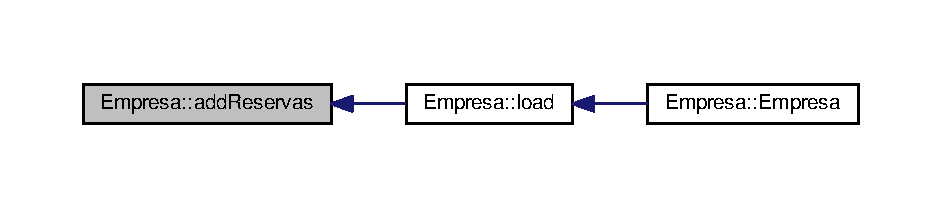
\includegraphics[width=350pt]{classEmpresa_a42a1671b234ab8380cfb2ed33517edb2_icgraph}
\end{center}
\end{figure}


\index{Empresa@{Empresa}!adiciona\+Cliente@{adiciona\+Cliente}}
\index{adiciona\+Cliente@{adiciona\+Cliente}!Empresa@{Empresa}}
\subsubsection[{\texorpdfstring{adiciona\+Cliente()}{adicionaCliente()}}]{\setlength{\rightskip}{0pt plus 5cm}void Empresa\+::adiciona\+Cliente (
\begin{DoxyParamCaption}
{}
\end{DoxyParamCaption}
)}\hypertarget{classEmpresa_aba4af6a945948ac66e771a416cfc2a2a}{}\label{classEmpresa_aba4af6a945948ac66e771a416cfc2a2a}


adds Clients 


\begin{DoxyCode}
142                               \{
143 
144 
145     \hyperlink{classEmpresa_ad79f7196a8ce7256771cbd7b9542155c}{titulo}();
146 
147     \textcolor{keywordtype}{int} opcaoRegisto;
148     \textcolor{keywordtype}{bool} clientechoice = \textcolor{keyword}{true};
149     \textcolor{keywordflow}{while} (clientechoice) \{
150 
151         cout << \textcolor{stringliteral}{"+----------------------------------------------------------+\(\backslash\)n"};
152         cout << \textcolor{stringliteral}{"| Pretende tornar-se um cliente registado?                 |\(\backslash\)n"};
153         cout << \textcolor{stringliteral}{"+----------------------------------------------------------+\(\backslash\)n"};
154         cout << \textcolor{stringliteral}{"| Selecione a sua opcao (insira apenas o numero):          |\(\backslash\)n"};
155         cout << \textcolor{stringliteral}{"+----------------------------------------------------------+\(\backslash\)n"};
156         cout << \textcolor{stringliteral}{"| 1 - Sim (tera conta registada e acumulara pontos)        |\(\backslash\)n"};
157         cout << \textcolor{stringliteral}{"| 2 - Nao (continuara como cliente normal)                 |\(\backslash\)n"};
158         cout << \textcolor{stringliteral}{"| 0 - Sair                                                 |\(\backslash\)n"};
159         cout << \textcolor{stringliteral}{"+----------------------------------------------------------+\(\backslash\)n"};
160         cin >> opcaoRegisto;
161         \textcolor{keywordflow}{if} (cin.fail())\{
162             cin.clear();
163             cin.ignore(INT\_MAX,\textcolor{charliteral}{'\(\backslash\)n'});
164             \hyperlink{menu_8h_aceb70c1ed7e11f0863a868704f02214b}{clearScreen}();
165             cout << \textcolor{stringliteral}{"Erro: Introduziu um input invalido. So pode usar numeros inteiros."} << endl;
166             cout << \textcolor{stringliteral}{"Pressione Enter para voltar ao menu"} << endl;
167             cin.get();
168         \}
169         \textcolor{keywordflow}{switch} (opcaoRegisto) \{
170         \textcolor{keywordflow}{case} 0:
171             \textcolor{keywordflow}{return};
172             \textcolor{keywordflow}{break};
173         \textcolor{keywordflow}{case} 1:
174             \hyperlink{classEmpresa_a430c00a63ef70338de3b4b7c096ea194}{adicionaClienteRegistado}();
175             clientechoice = \textcolor{keyword}{false};
176             \textcolor{keywordflow}{break};
177         \textcolor{keywordflow}{case} 2:
178             \hyperlink{classEmpresa_a372599c8aee20690517cc3ae6c8e1ca7}{adicionaClienteNormal}();
179             clientechoice = \textcolor{keyword}{false};
180             \textcolor{keywordflow}{break};
181         \textcolor{keywordflow}{default}:
182             cout << \textcolor{stringliteral}{"Lamento, mas a opcao que inseriu nao e valida. Sera redirecionado/a para o inicio do
       menu. \(\backslash\)n"};
183         \}
184 
185     \}
186 
187 
188 \}
\end{DoxyCode}
\index{Empresa@{Empresa}!adiciona\+Cliente\+Normal@{adiciona\+Cliente\+Normal}}
\index{adiciona\+Cliente\+Normal@{adiciona\+Cliente\+Normal}!Empresa@{Empresa}}
\subsubsection[{\texorpdfstring{adiciona\+Cliente\+Normal()}{adicionaClienteNormal()}}]{\setlength{\rightskip}{0pt plus 5cm}void Empresa\+::adiciona\+Cliente\+Normal (
\begin{DoxyParamCaption}
{}
\end{DoxyParamCaption}
)}\hypertarget{classEmpresa_a372599c8aee20690517cc3ae6c8e1ca7}{}\label{classEmpresa_a372599c8aee20690517cc3ae6c8e1ca7}


displays the interface to add Clients 


\begin{DoxyCode}
190                                     \{
191 
192     \hyperlink{classEmpresa_ad79f7196a8ce7256771cbd7b9542155c}{titulo}();
193     \textcolor{keywordtype}{string} nomeCliente;
194     \textcolor{keywordtype}{string} morada;
195 
196     cout << \textcolor{stringliteral}{"+----------------------------------------------------------+\(\backslash\)n"};
197     cout << \textcolor{stringliteral}{"| Qual e o seu nome?                                       |\(\backslash\)n"};
198     cout << \textcolor{stringliteral}{"+----------------------------------------------------------+\(\backslash\)n"};
199 
200     cin.ignore (INT\_MAX,\textcolor{charliteral}{'\(\backslash\)n'});
201     getline(cin,nomeCliente);
202 
203     \textcolor{keywordflow}{if}(\hyperlink{extras_8h_abc85c93edf561168b5bbee8054caa388}{BinarySearch}(this->\_clientes,nomeCliente) != -1)\{
204         \textcolor{keywordflow}{throw} \hyperlink{classObjetoRepetido}{ObjetoRepetido<Cliente>}(nomeCliente);
205     \}
206 
207     cout << \textcolor{stringliteral}{"+----------------------------------------------------------+\(\backslash\)n"};
208     cout << \textcolor{stringliteral}{"| Qual a sua morada?                                       |\(\backslash\)n"};
209     cout << \textcolor{stringliteral}{"+----------------------------------------------------------+\(\backslash\)n"};
210 
211     getline(cin,morada);
212 
213     \hyperlink{classCliente}{Cliente} * novocliente = \textcolor{keyword}{new} \hyperlink{classCliente}{Cliente}(nomeCliente, morada);
214     \hyperlink{classEmpresa_a57597ec4154f274686bc648ccf5d2a59}{addClientes}(*novocliente);
215     this->\hyperlink{classEmpresa_aa7424cde3bdf1b1921967bc176d0ab50}{sort}();
216     \textcolor{keywordflow}{return};
217 
218 \}
\end{DoxyCode}


Here is the call graph for this function\+:\nopagebreak
\begin{figure}[H]
\begin{center}
\leavevmode
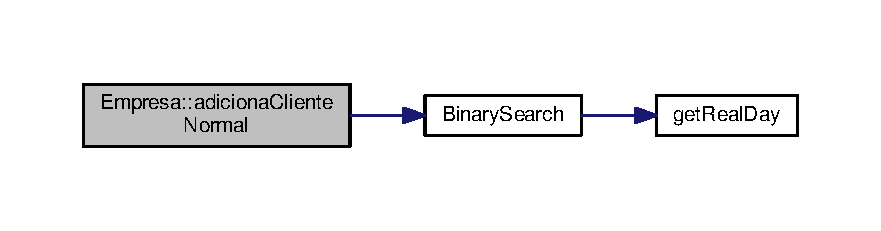
\includegraphics[width=350pt]{classEmpresa_a372599c8aee20690517cc3ae6c8e1ca7_cgraph}
\end{center}
\end{figure}


\index{Empresa@{Empresa}!adiciona\+Cliente\+Registado@{adiciona\+Cliente\+Registado}}
\index{adiciona\+Cliente\+Registado@{adiciona\+Cliente\+Registado}!Empresa@{Empresa}}
\subsubsection[{\texorpdfstring{adiciona\+Cliente\+Registado()}{adicionaClienteRegistado()}}]{\setlength{\rightskip}{0pt plus 5cm}void Empresa\+::adiciona\+Cliente\+Registado (
\begin{DoxyParamCaption}
{}
\end{DoxyParamCaption}
)}\hypertarget{classEmpresa_a430c00a63ef70338de3b4b7c096ea194}{}\label{classEmpresa_a430c00a63ef70338de3b4b7c096ea194}


displays the interface to add Registred Clients 


\begin{DoxyCode}
220                                        \{
221 
222     \hyperlink{classEmpresa_ad79f7196a8ce7256771cbd7b9542155c}{titulo}();
223     \textcolor{keywordtype}{string} nomeClienteRegistado;
224     \textcolor{keywordtype}{string} morada;
225 
226     cout << \textcolor{stringliteral}{"+----------------------------------------------------------+\(\backslash\)n"};
227     cout << \textcolor{stringliteral}{"| Com que nome pretende ficar registado?                   |\(\backslash\)n"};
228     cout << \textcolor{stringliteral}{"+----------------------------------------------------------+\(\backslash\)n"};
229 
230     cin.ignore(INT\_MAX, \textcolor{charliteral}{'\(\backslash\)n'});
231     getline(cin,nomeClienteRegistado);
232     \textcolor{keywordflow}{if}(\hyperlink{extras_8h_abc85c93edf561168b5bbee8054caa388}{BinarySearch}(this->\_clientes,nomeClienteRegistado) != -1)\{
233         \textcolor{keywordflow}{throw} \hyperlink{classObjetoRepetido}{ObjetoRepetido<Cliente>}(nomeClienteRegistado);
234     \}
235 
236     cout << \textcolor{stringliteral}{"+----------------------------------------------------------+\(\backslash\)n"};
237     cout << \textcolor{stringliteral}{"| Qual a sua morada?                                       |\(\backslash\)n"};
238     cout << \textcolor{stringliteral}{"+----------------------------------------------------------+\(\backslash\)n"};
239 
240     getline(cin,morada);
241 
242     \hyperlink{classCliente}{Cliente} * novoClienteRegistado = \textcolor{keyword}{new} \hyperlink{classClienteRegistado}{ClienteRegistado}(nomeClienteRegistado,
      morada, 0);
243     \hyperlink{classEmpresa_a57597ec4154f274686bc648ccf5d2a59}{addClientes}(*novoClienteRegistado);
244     this->\hyperlink{classEmpresa_aa7424cde3bdf1b1921967bc176d0ab50}{sort}();
245     cout << \textcolor{stringliteral}{"Pressione Enter para regressar\(\backslash\)n"};
246     cin.get();
247     \textcolor{keywordflow}{return};
248 
249 \}
\end{DoxyCode}


Here is the call graph for this function\+:\nopagebreak
\begin{figure}[H]
\begin{center}
\leavevmode
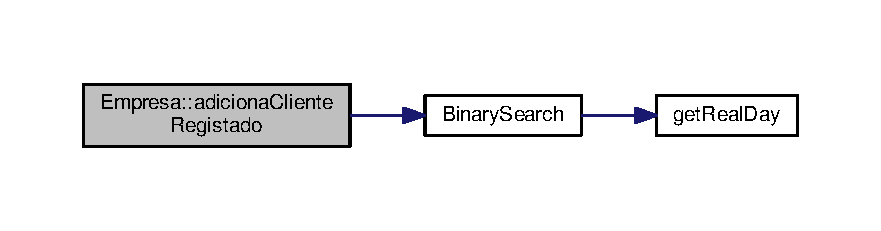
\includegraphics[width=350pt]{classEmpresa_a430c00a63ef70338de3b4b7c096ea194_cgraph}
\end{center}
\end{figure}


\index{Empresa@{Empresa}!adiciona\+Fornecedor@{adiciona\+Fornecedor}}
\index{adiciona\+Fornecedor@{adiciona\+Fornecedor}!Empresa@{Empresa}}
\subsubsection[{\texorpdfstring{adiciona\+Fornecedor()}{adicionaFornecedor()}}]{\setlength{\rightskip}{0pt plus 5cm}void Empresa\+::adiciona\+Fornecedor (
\begin{DoxyParamCaption}
{}
\end{DoxyParamCaption}
)}\hypertarget{classEmpresa_af20261a3f95a5dd0c4a5a796d9a3d442}{}\label{classEmpresa_af20261a3f95a5dd0c4a5a796d9a3d442}


displays the interface to add suppliers 


\begin{DoxyCode}
517                                  \{
518 
519     \hyperlink{classEmpresa_ad79f7196a8ce7256771cbd7b9542155c}{titulo}();
520     \textcolor{keywordtype}{string} nome\_fornecedor, morada;
521     \textcolor{keywordtype}{int} NIF;
522 
523     cout << \textcolor{stringliteral}{"+----------------------------------------------------------+\(\backslash\)n"};
524     cout << \textcolor{stringliteral}{"| Qual e o nome do fornecedor?                             |\(\backslash\)n"};
525     cout << \textcolor{stringliteral}{"+----------------------------------------------------------+\(\backslash\)n"};
526 
527     cin.ignore(INT\_MAX,\textcolor{charliteral}{'\(\backslash\)n'});
528     getline(cin,nome\_fornecedor);
529     \textcolor{keywordflow}{if}(\hyperlink{extras_8h_abc85c93edf561168b5bbee8054caa388}{BinarySearch}(this->\_fornecedores,nome\_fornecedor) != -1)\{
530         \textcolor{keywordflow}{throw} \hyperlink{classObjetoRepetido}{ObjetoRepetido<Fornecedor>}(nome\_fornecedor);
531     \}
532 
533     cout << \textcolor{stringliteral}{"+----------------------------------------------------------+\(\backslash\)n"};
534     cout << \textcolor{stringliteral}{"| Indique o NIF:                                           |\(\backslash\)n"};
535     cout << \textcolor{stringliteral}{"+----------------------------------------------------------+\(\backslash\)n"};
536 
537     cin >> NIF;
538 
539     cout << \textcolor{stringliteral}{"+----------------------------------------------------------+\(\backslash\)n"};
540     cout << \textcolor{stringliteral}{"| Indique a morada:                                        |\(\backslash\)n"};
541     cout << \textcolor{stringliteral}{"+----------------------------------------------------------+\(\backslash\)n"};
542 
543     cin.ignore(INT\_MAX,\textcolor{charliteral}{'\(\backslash\)n'});
544     getline(cin,morada);
545     \hyperlink{classFornecedor}{Fornecedor} * novoFornecedor = \textcolor{keyword}{new} \hyperlink{classFornecedor}{Fornecedor}(nome\_fornecedor, NIF, morada);
546     novoFornecedor->\hyperlink{classFornecedor_a0a0945cbd2fd120d9eab5d5aec441b72}{setDefinicoesFornecedor}();
547     \hyperlink{classEmpresa_a0c858479d6e92094adbb2fc085039376}{addFornecedores}(*novoFornecedor);
548     this->\hyperlink{classEmpresa_aa7424cde3bdf1b1921967bc176d0ab50}{sort}();
549 \}
\end{DoxyCode}


Here is the call graph for this function\+:\nopagebreak
\begin{figure}[H]
\begin{center}
\leavevmode
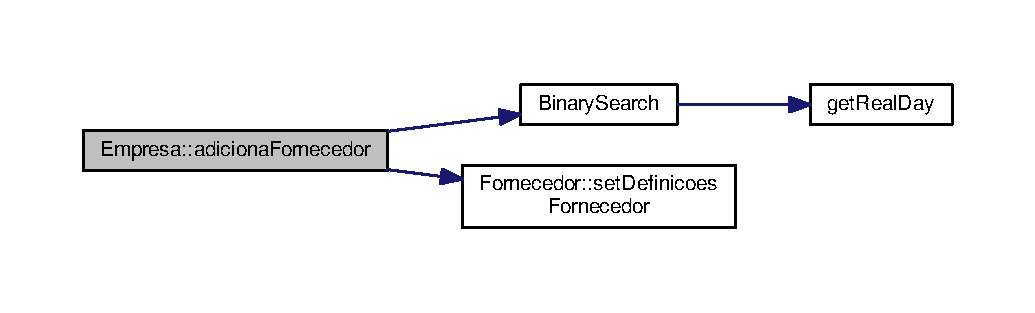
\includegraphics[width=350pt]{classEmpresa_af20261a3f95a5dd0c4a5a796d9a3d442_cgraph}
\end{center}
\end{figure}


\index{Empresa@{Empresa}!adiciona\+Oferta@{adiciona\+Oferta}}
\index{adiciona\+Oferta@{adiciona\+Oferta}!Empresa@{Empresa}}
\subsubsection[{\texorpdfstring{adiciona\+Oferta()}{adicionaOferta()}}]{\setlength{\rightskip}{0pt plus 5cm}void Empresa\+::adiciona\+Oferta (
\begin{DoxyParamCaption}
{}
\end{DoxyParamCaption}
)}\hypertarget{classEmpresa_ae244a8ae3afb85eb5e9e5febce8b8728}{}\label{classEmpresa_ae244a8ae3afb85eb5e9e5febce8b8728}


displays the interface to adds offers 


\begin{DoxyCode}
1457                              \{
1458 
1459     \hyperlink{classEmpresa_ad79f7196a8ce7256771cbd7b9542155c}{titulo}();
1460     std::string nome;
1461     std::string barco;
1462     \textcolor{keywordtype}{int} numeroBarco;
1463     std::string temp;
1464     std::vector<std::string> destinos;
1465     \hyperlink{classOferta}{Oferta} * novaOferta;
1466     \textcolor{keywordtype}{unsigned} \textcolor{keywordtype}{int} distancia;
1467     \textcolor{keywordtype}{unsigned} \textcolor{keywordtype}{int} preco;
1468     \textcolor{keywordtype}{int} lotacao;
1469     std::string data;
1470     \hyperlink{classTime}{Time} * tempo;
1471     \textcolor{keywordtype}{int} index;
1472 
1473     \hyperlink{classEmpresa_a55c3756c01b45b41ad03f4e4f3e4dcac}{displayFornecedores}();
1474 
1475     cout << \textcolor{stringliteral}{"+----------------------------------------------------------+\(\backslash\)n"};
1476     cout << \textcolor{stringliteral}{"| Qual e o nome do fornecedor?                             |\(\backslash\)n"};
1477     cout << \textcolor{stringliteral}{"+----------------------------------------------------------+\(\backslash\)n"};
1478 
1479     cin.ignore(INT\_MAX,\textcolor{charliteral}{'\(\backslash\)n'});
1480     getline(cin,nome);
1481     index = \hyperlink{extras_8h_abc85c93edf561168b5bbee8054caa388}{BinarySearch}(this->\_fornecedores,nome);
1482     \textcolor{keywordflow}{if}(index == -1)\{
1483         \textcolor{keywordflow}{throw} \hyperlink{classObjetoInexistente}{ObjetoInexistente<Fornecedor>}(nome);
1484     \}
1485     
1486 
1487     cout << \textcolor{stringliteral}{"+----------------------------------------------------------+\(\backslash\)n"};
1488     cout << \textcolor{stringliteral}{"| Qual e o nome da oferta?                                 |\(\backslash\)n"};
1489     cout << \textcolor{stringliteral}{"+----------------------------------------------------------+\(\backslash\)n"};
1490 
1491     getline(cin,nome);
1492 
1493     cout << \textcolor{stringliteral}{"+----------------------------------------------------------+\(\backslash\)n"};
1494     cout << \textcolor{stringliteral}{"| Escolha o tipo de barco:                                 |\(\backslash\)n"};
1495     cout << \textcolor{stringliteral}{"+----------------------------------------------------------+\(\backslash\)n"};
1496     cout << \textcolor{stringliteral}{"| 1 - Iate                                                 |\(\backslash\)n"};
1497     cout << \textcolor{stringliteral}{"| 2 - Barco rabelo                                         |\(\backslash\)n"};
1498     cout << \textcolor{stringliteral}{"| 3 - Veleiro                                              |\(\backslash\)n"};
1499     cout << \textcolor{stringliteral}{"+----------------------------------------------------------+\(\backslash\)n"};
1500 
1501     cin >> numeroBarco;
1502     \textcolor{keywordflow}{switch} (numeroBarco) \{
1503     \textcolor{keywordflow}{case} 1: 
1504         barco = \textcolor{stringliteral}{"iate"};
1505         \textcolor{keywordflow}{break};
1506     \textcolor{keywordflow}{case} 2:
1507         barco = \textcolor{stringliteral}{"barco rabelo"};
1508         \textcolor{keywordflow}{break};
1509     \textcolor{keywordflow}{case} 3:
1510         barco = \textcolor{stringliteral}{"veleiro"};
1511         \textcolor{keywordflow}{break};
1512     \textcolor{keywordflow}{default}:
1513         cout << \textcolor{stringliteral}{"Esse número nao é reconhecido como barco."};
1514         
1515 
1516     \}
1517 
1518 
1519 
1520     cout << \textcolor{stringliteral}{"+----------------------------------------------------------+\(\backslash\)n"};
1521     cout << \textcolor{stringliteral}{"| Indique os destinos (escreva FIM quando terminar):       |\(\backslash\)n"};
1522     cout << \textcolor{stringliteral}{"+----------------------------------------------------------+\(\backslash\)n"};
1523     cin.ignore(INT\_MAX,\textcolor{charliteral}{'\(\backslash\)n'});
1524     \textcolor{keywordflow}{while} (temp != \textcolor{stringliteral}{"FIM"})
1525     \{
1526         getline(cin,temp);
1527         \textcolor{keywordflow}{if}(temp != \textcolor{stringliteral}{"FIM"})\{
1528          destinos.push\_back(temp);
1529         \}
1530         cout << \textcolor{stringliteral}{"\(\backslash\)n"};
1531     \}
1532 
1533     cout << \textcolor{stringliteral}{"+----------------------------------------------------------+\(\backslash\)n"};
1534     cout << \textcolor{stringliteral}{"| Indique a distancia total percorrida:                    |\(\backslash\)n"};
1535     cout << \textcolor{stringliteral}{"+----------------------------------------------------------+\(\backslash\)n"};
1536 
1537     cin >> distancia;
1538 
1539     cout << \textcolor{stringliteral}{"+----------------------------------------------------------+\(\backslash\)n"};
1540     cout << \textcolor{stringliteral}{"| Indique a lotacao total do barco:                        |\(\backslash\)n"};
1541     cout << \textcolor{stringliteral}{"+----------------------------------------------------------+\(\backslash\)n"};
1542 
1543     cin >> lotacao;
1544 
1545     cout << \textcolor{stringliteral}{"+----------------------------------------------------------+\(\backslash\)n"};
1546     cout << \textcolor{stringliteral}{"| Indique a data da viagem (YY/MM/DD H:M):                 |\(\backslash\)n"};
1547     cout << \textcolor{stringliteral}{"+----------------------------------------------------------+\(\backslash\)n"};
1548 
1549     cin.ignore(INT\_MAX,\textcolor{charliteral}{'\(\backslash\)n'});
1550     getline(cin,data);
1551     tempo = \textcolor{keyword}{new} \hyperlink{classTime}{Time}(data);
1552 
1553     preco = \_fornecedores.at(index)->calculaPreco(numeroBarco, lotacao, distancia);
1554     
1555     
1556     novaOferta = \textcolor{keyword}{new} \hyperlink{classOferta}{Oferta}(nome, barco, destinos, distancia, lotacao, *tempo, preco);
1557 
1558     \textcolor{keywordflow}{for} (\textcolor{keywordtype}{unsigned} \textcolor{keywordtype}{int} i = 0; i < \_fornecedores.size(); i++)
1559     \{
1560         \textcolor{keywordflow}{for} (\textcolor{keywordtype}{unsigned} \textcolor{keywordtype}{int} j = 0; j < \_fornecedores[i]->getOfertas().size(); j++)
1561         \{
1562             \textcolor{keywordflow}{if} (\_fornecedores[i]->getOfertas().at(j).getBarcoNumber() == novaOferta->
      \hyperlink{classOferta_abf0f062fa730edf6d4232926980b106c}{getBarcoNumber}())\{
1563                 \_fornecedores[i]->getOfertas().at(j).setTimeUltimaReserva(novaOferta->
      \hyperlink{classOferta_a1caf2c681c14c9fbd04312b35f99b64c}{getUltimaReserva}());
1564         \}
1565         \}
1566     \}
1567     this->\_fornecedores[index]->addOferta(*novaOferta);
1568 
1569     \hyperlink{classEmpresa_a5ca8821d938f11f29558ae90913de528}{addOfertasQueue}();
1570     \hyperlink{classEmpresa_a46a4898b8ae8e09bdf656b25b8ffe99d}{aplicaDesconto}();
1571 
1572 \}
\end{DoxyCode}


Here is the call graph for this function\+:\nopagebreak
\begin{figure}[H]
\begin{center}
\leavevmode
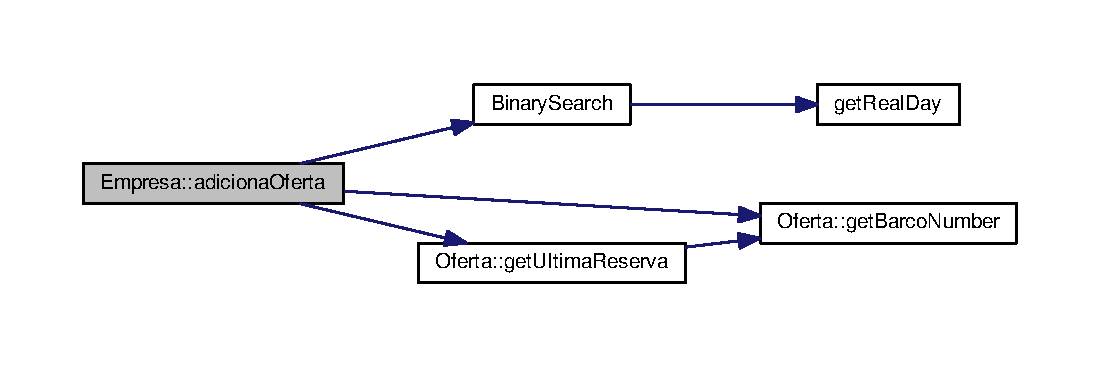
\includegraphics[width=350pt]{classEmpresa_ae244a8ae3afb85eb5e9e5febce8b8728_cgraph}
\end{center}
\end{figure}


\index{Empresa@{Empresa}!adiciona\+Reserva@{adiciona\+Reserva}}
\index{adiciona\+Reserva@{adiciona\+Reserva}!Empresa@{Empresa}}
\subsubsection[{\texorpdfstring{adiciona\+Reserva()}{adicionaReserva()}}]{\setlength{\rightskip}{0pt plus 5cm}void Empresa\+::adiciona\+Reserva (
\begin{DoxyParamCaption}
{}
\end{DoxyParamCaption}
)}\hypertarget{classEmpresa_a42953bdbb2fb39173ad6f38892fc122b}{}\label{classEmpresa_a42953bdbb2fb39173ad6f38892fc122b}


displays the interface to add reservations 


\begin{DoxyCode}
918                               \{
919 
920     \hyperlink{classEmpresa_ad79f7196a8ce7256771cbd7b9542155c}{titulo}();
921     \textcolor{keywordtype}{string} nome\_fornecedor, nomeCliente, nomeOferta;
922     \textcolor{keywordtype}{unsigned} \textcolor{keywordtype}{int}  preco,lotacao;
923     \textcolor{keywordtype}{unsigned} \textcolor{keywordtype}{int} pontos;
924     \textcolor{keywordtype}{bool} cancelada = \textcolor{keyword}{false};
925     \textcolor{keywordtype}{bool} erroNome = \textcolor{keyword}{true};
926     vector<Oferta*> ofertas;
927 
928     
929     cout << \textcolor{stringliteral}{"+----------------------------------------------------------+\(\backslash\)n"};
930     cout << \textcolor{stringliteral}{"| Estes sao os clientes:                                   |\(\backslash\)n"};
931     cout << \textcolor{stringliteral}{"+----------------------------------------------------------+\(\backslash\)n"};
932 
933     \hyperlink{classEmpresa_a28e04d59daa7206bec6055249ce17410}{displayClientes}();
934 
935     cout << \textcolor{stringliteral}{"+----------------------------------------------------------+\(\backslash\)n"};
936     cout << \textcolor{stringliteral}{"| Indique o nome do cliente:                               |\(\backslash\)n"};
937     cout << \textcolor{stringliteral}{"+----------------------------------------------------------+\(\backslash\)n"};
938     cin.ignore(INT\_MAX,\textcolor{charliteral}{'\(\backslash\)n'});
939     getline(cin, nomeCliente);
940 
941     \textcolor{keywordtype}{int} indexCliente = \hyperlink{extras_8h_abc85c93edf561168b5bbee8054caa388}{BinarySearch}(\_clientes, nomeCliente);
942 
943     \textcolor{keywordflow}{if} (indexCliente == -1) \{ \textcolor{keywordflow}{throw} \hyperlink{classObjetoInexistente}{ObjetoInexistente<Cliente>}(nomeCliente); \}
944 
945     
946     cout << \textcolor{stringliteral}{"+----------------------------------------------------------+\(\backslash\)n"};
947     cout << \textcolor{stringliteral}{"| Estes sao todos os fornecedores e respetivas ofertas     |\(\backslash\)n"};
948     cout << \textcolor{stringliteral}{"+----------------------------------------------------------+\(\backslash\)n"};
949     
950     \hyperlink{classEmpresa_aa47e9a64800a41180b7f374b73a1f32b}{displayFornecedorescomOfertas}();
951 
952     cout << \textcolor{stringliteral}{"+----------------------------------------------------------+\(\backslash\)n"};
953     cout << \textcolor{stringliteral}{"| Indique o nome do fornecedor:                            |\(\backslash\)n"};
954     cout << \textcolor{stringliteral}{"+----------------------------------------------------------+\(\backslash\)n"};
955 
956 
957     getline(cin, nome\_fornecedor);
958     \textcolor{keywordtype}{int} index = \hyperlink{extras_8h_abc85c93edf561168b5bbee8054caa388}{BinarySearch}(\_fornecedores, nome\_fornecedor);
959 
960     \textcolor{keywordflow}{if} (index == -1) \{ \textcolor{keywordflow}{throw} \hyperlink{classObjetoInexistente}{ObjetoInexistente<Fornecedor>}(nome\_fornecedor); \}
961 
962 
963     cout << \textcolor{stringliteral}{"+----------------------------------------------------------+\(\backslash\)n"};
964     cout << \textcolor{stringliteral}{"| Estas sao as suas ofertas:                               |\(\backslash\)n"};
965     cout << \textcolor{stringliteral}{"+----------------------------------------------------------+\(\backslash\)n"};
966 
967     \_fornecedores.at(index)->displayOfertas();
968 
969     cout << \textcolor{stringliteral}{"+----------------------------------------------------------+\(\backslash\)n"};
970     cout << \textcolor{stringliteral}{"| Indique o nome da oferta que pretende reservar:          |\(\backslash\)n"};
971     cout << \textcolor{stringliteral}{"+----------------------------------------------------------+\(\backslash\)n"};
972     
973     getline(cin, nomeOferta);
974 
975     \textcolor{keywordflow}{for} (\textcolor{keywordtype}{unsigned} \textcolor{keywordtype}{int} k = 0; k < \_fornecedores.at(index)->getOfertas().size(); k++)
976     \{
977         \textcolor{keywordflow}{if} (\_fornecedores.at(index)->getOfertas().at(k).getNome() == nomeOferta)
978         \{
979             ofertas.push\_back(&\_fornecedores.at(index)->getOfertas()[k]);
980             erroNome = \textcolor{keyword}{false};
981 
982         \}
983 
984     \}
985 
986     \textcolor{keywordflow}{if} (erroNome)
987     \{
988         \textcolor{keywordflow}{throw} \hyperlink{classObjetoInexistente}{ObjetoInexistente<Oferta>}(nomeOferta);
989     \}
990 
991     cout << \textcolor{stringliteral}{"+----------------------------------------------------------+\(\backslash\)n"};
992     cout << \textcolor{stringliteral}{"| Indique para quantas pessoas quer efetuar a reserva:     |\(\backslash\)n"};
993     cout << \textcolor{stringliteral}{"+----------------------------------------------------------+\(\backslash\)n"};
994 
995     cin >> lotacao;
996 
997     \textcolor{keywordflow}{if} (lotacao <= ofertas[0]->getLotacao())
998         ofertas[0]->diminuiLotacao(lotacao);
999     \textcolor{keywordflow}{else} \{
1000         cout << \textcolor{stringliteral}{"Esse numero de pessoas excede o limite na oferta. Pressione Enter regressar."};
1001         cin.get();
1002         \textcolor{keywordflow}{return};
1003     \}
1004 
1005     cin.get();
1006 
1007     preco = \_fornecedores.at(index)->calculaPreco(ofertas[0]->getBarcoNumber(), lotacao, ofertas[0]->
      getDistancia());
1008 
1009     \textcolor{comment}{//se os clientes tiverem 0 pontos, acumulam 1/5 do preço da viagem em pontos}
1010     \textcolor{comment}{//se eles tiverem pontos inferiores à viagem, gastam todos e ficam set a 0, mas o custo é reduzido em
       numero igual aos pontos}
1011     \textcolor{comment}{//se tiverem superior, gastam até cobrir o custo da viagem, e têm a viagem de graça}
1012 
1013     pontos = \_clientes.at(indexCliente)->getPontos();
1014         \textcolor{keywordflow}{if} (\_clientes.at(indexCliente)->getPontos() == 0)
1015         \{
1016             pontos = preco / 5;
1017             
1018         \}
1019         \textcolor{keywordflow}{else} \textcolor{keywordflow}{if} (\_clientes.at(indexCliente)->getPontos() <= preco)
1020         \{
1021             preco = preco - \_clientes.at(indexCliente)->getPontos();
1022             pontos = 0;
1023             
1024         \}
1025         \textcolor{keywordflow}{else} \{ \textcolor{comment}{// (\_clientes.at(indexCliente)->getPontos() > preco)}
1026             
1027             pontos = pontos - preco;
1028             preco = 0;
1029             
1030             
1031         \}
1032         \_clientes.at(indexCliente)->setPontos(pontos);
1033         
1034     
1035     
1036     
1037 
1038     \hyperlink{classReserva}{Reserva} * novaReserva = \textcolor{keyword}{new} \hyperlink{classReserva}{Reserva}(nome\_fornecedor, ofertas[0], nomeCliente, \_clientes.
      at(indexCliente), preco, cancelada);
1039     \hyperlink{classEmpresa_a42a1671b234ab8380cfb2ed33517edb2}{addReservas}(*novaReserva);  
1040     \hyperlink{classFatura}{Fatura} novaFatura(novaReserva);
1041     this->\_faturas.\hyperlink{classBST_a2b117df6521c7d61dac75ff2c938bae7}{insert}(novaFatura);
1042     \hyperlink{classRealTime}{RealTime} tempoReserva;
1043     \textcolor{keywordflow}{for} (\textcolor{keywordtype}{unsigned} \textcolor{keywordtype}{int} l = 0; l < \_fornecedores.at(index)->getOfertas().size(); l++)
1044     \{
1045         \textcolor{keywordflow}{if} (\_fornecedores.at(index)->getOfertas().at(l).getBarcoNumber() == ofertas[0]->getBarcoNumber())
1046         \{
1047             \_fornecedores.at(index)->getOfertas().at(l).setTimeUltimaReserva(tempoReserva);
1048 
1049         \}
1050     \}
1051     \hyperlink{classClienteInativo}{ClienteInativo} * ci = \textcolor{keyword}{new} \hyperlink{classClienteInativo}{ClienteInativo}(this->\_clientes[indexCliente]);
1052         this->\_clientesInativos.erase(*ci);
1053     cout << \textcolor{stringliteral}{"+----------------------------------------------------------+\(\backslash\)n"};
1054     cout << \textcolor{stringliteral}{"| A oferta foi reservada com sucesso.                      |\(\backslash\)n"};
1055     cout << \textcolor{stringliteral}{"+----------------------------------------------------------+\(\backslash\)n"};
1056     this->\hyperlink{classEmpresa_aa7424cde3bdf1b1921967bc176d0ab50}{sort}();
1057 
1058     \hyperlink{classEmpresa_a5ca8821d938f11f29558ae90913de528}{addOfertasQueue}();
1059     \hyperlink{classEmpresa_a46a4898b8ae8e09bdf656b25b8ffe99d}{aplicaDesconto}();
1060 
1061 \}
\end{DoxyCode}


Here is the call graph for this function\+:\nopagebreak
\begin{figure}[H]
\begin{center}
\leavevmode
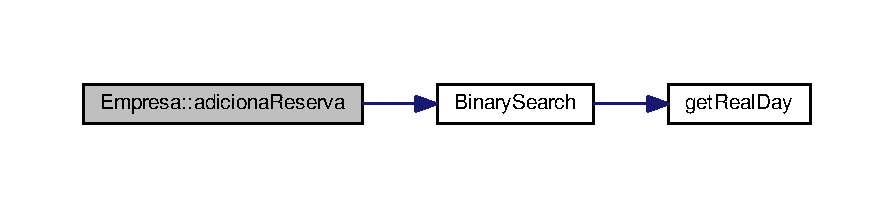
\includegraphics[width=350pt]{classEmpresa_a42953bdbb2fb39173ad6f38892fc122b_cgraph}
\end{center}
\end{figure}


\index{Empresa@{Empresa}!aplica\+Desconto@{aplica\+Desconto}}
\index{aplica\+Desconto@{aplica\+Desconto}!Empresa@{Empresa}}
\subsubsection[{\texorpdfstring{aplica\+Desconto()}{aplicaDesconto()}}]{\setlength{\rightskip}{0pt plus 5cm}void Empresa\+::aplica\+Desconto (
\begin{DoxyParamCaption}
{}
\end{DoxyParamCaption}
)}\hypertarget{classEmpresa_a46a4898b8ae8e09bdf656b25b8ffe99d}{}\label{classEmpresa_a46a4898b8ae8e09bdf656b25b8ffe99d}


Applies discount. 


\begin{DoxyCode}
592                              \{
593     \textcolor{keywordtype}{int} antigopreco;
594     
595     \hyperlink{classOferta}{Oferta} ofertatemp = queueOfertasOrdenadas.top();
596     antigopreco = ofertatemp.\hyperlink{classOferta_a6237afc2e8a33fb55b1ef0decf9d9aaa}{getPreco}();
597     ofertatemp.\hyperlink{classOferta_a900c1febcd11221d877bc7cce577dd18}{setPreco}(antigopreco*0.8);
598     queueOfertasOrdenadas.pop();
599     queueOfertasOrdenadas.push(ofertatemp);
600 \}
\end{DoxyCode}


Here is the call graph for this function\+:\nopagebreak
\begin{figure}[H]
\begin{center}
\leavevmode
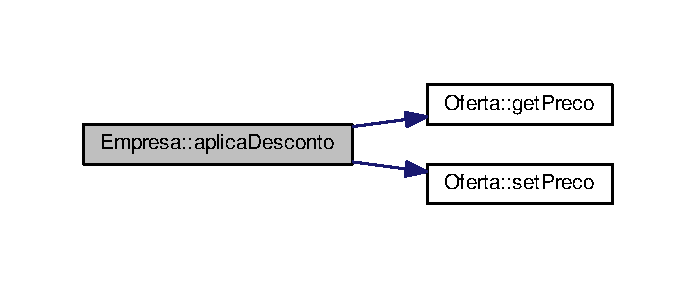
\includegraphics[width=334pt]{classEmpresa_a46a4898b8ae8e09bdf656b25b8ffe99d_cgraph}
\end{center}
\end{figure}


\index{Empresa@{Empresa}!atualiza\+Inatividade@{atualiza\+Inatividade}}
\index{atualiza\+Inatividade@{atualiza\+Inatividade}!Empresa@{Empresa}}
\subsubsection[{\texorpdfstring{atualiza\+Inatividade()}{atualizaInatividade()}}]{\setlength{\rightskip}{0pt plus 5cm}{\bf Empresa} \& Empresa\+::atualiza\+Inatividade (
\begin{DoxyParamCaption}
{}
\end{DoxyParamCaption}
)}\hypertarget{classEmpresa_aea372dbf680408d9fb32341c03b3e5ad}{}\label{classEmpresa_aea372dbf680408d9fb32341c03b3e5ad}


Updates which clients are inactive. 

\begin{DoxyReturn}{Returns}
The modified empresa 
\end{DoxyReturn}

\begin{DoxyCode}
610                                       \{
611     \hyperlink{classTime}{Time} ultimaReserva;
612     \hyperlink{classRealTime}{RealTime} rt;
613     \hyperlink{classClienteInativo}{ClienteInativo} * ci;
614     \textcolor{keywordflow}{for}(\textcolor{keywordtype}{unsigned} \textcolor{keywordtype}{int} i = 0; i < this->\_reservas.size(); i++)\{
615         ci = \textcolor{keyword}{new} \hyperlink{classClienteInativo}{ClienteInativo}(this->\_reservas[i]->getCliente());
616         \textcolor{keywordflow}{if}(this->\_clientesInativos.find(*ci) != this->\_clientesInativos.end())\{
617                 \textcolor{keywordflow}{continue};
618         \}
619         \textcolor{keywordflow}{if}(this->\_reservas[i]->getData().diferencaDias() > (6*30))\{
620             this->\_clientesInativos.insert(*ci);
621         \}
622 
623     \}
624 
625     \textcolor{keywordflow}{return} *\textcolor{keyword}{this};
626 \}
\end{DoxyCode}


Here is the call graph for this function\+:\nopagebreak
\begin{figure}[H]
\begin{center}
\leavevmode
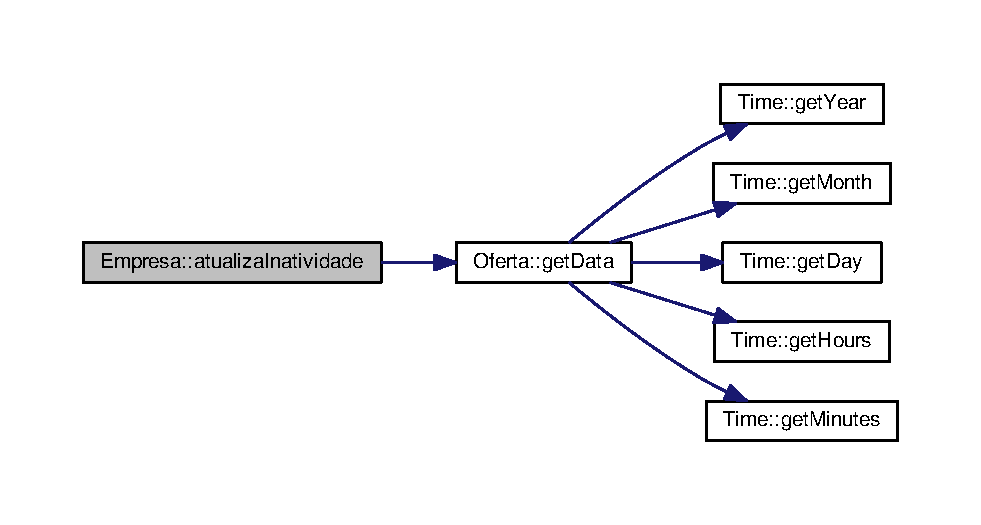
\includegraphics[width=350pt]{classEmpresa_aea372dbf680408d9fb32341c03b3e5ad_cgraph}
\end{center}
\end{figure}




Here is the caller graph for this function\+:\nopagebreak
\begin{figure}[H]
\begin{center}
\leavevmode
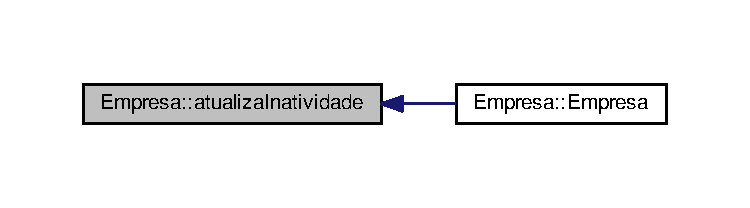
\includegraphics[width=350pt]{classEmpresa_aea372dbf680408d9fb32341c03b3e5ad_icgraph}
\end{center}
\end{figure}


\index{Empresa@{Empresa}!cancela\+Reservas@{cancela\+Reservas}}
\index{cancela\+Reservas@{cancela\+Reservas}!Empresa@{Empresa}}
\subsubsection[{\texorpdfstring{cancela\+Reservas()}{cancelaReservas()}}]{\setlength{\rightskip}{0pt plus 5cm}void Empresa\+::cancela\+Reservas (
\begin{DoxyParamCaption}
{}
\end{DoxyParamCaption}
)}\hypertarget{classEmpresa_aa0b169a112c75b6fd1bc80128720282e}{}\label{classEmpresa_aa0b169a112c75b6fd1bc80128720282e}


displays the interface to cancel reservations 


\begin{DoxyCode}
1190                               \{
1191     \hyperlink{classEmpresa_ad79f7196a8ce7256771cbd7b9542155c}{titulo}();
1192     \textcolor{keywordtype}{int} novoPreco;
1193     \textcolor{keywordtype}{bool} nfound = \textcolor{keyword}{true};
1194 
1195     cout << \textcolor{stringliteral}{"+----------------------------------------------------------+\(\backslash\)n"};
1196     cout << \textcolor{stringliteral}{"| Estas sao as reservas disponíveis:                       |\(\backslash\)n"};
1197     cout << \textcolor{stringliteral}{"+----------------------------------------------------------+\(\backslash\)n"};
1198 
1199     \hyperlink{classEmpresa_a8c89e6053eaccf0e1938a4f2ab0bfdc4}{displayReservas}();
1200 
1201     \textcolor{keywordtype}{string} reservaremoveOferta,reservaremoveCliente;
1202     cout << \textcolor{stringliteral}{"+----------------------------------------------------------+\(\backslash\)n"};
1203     cout << \textcolor{stringliteral}{"| Indique o nome do cliente cuja oferta quer cancelar      |\(\backslash\)n"};
1204     cout << \textcolor{stringliteral}{"+----------------------------------------------------------+\(\backslash\)n"};
1205 
1206     cin.ignore(INT\_MAX,\textcolor{charliteral}{'\(\backslash\)n'});
1207     getline(cin,reservaremoveCliente);
1208     
1209     cout << \textcolor{stringliteral}{"+----------------------------------------------------------+\(\backslash\)n"};
1210     cout << \textcolor{stringliteral}{"| Indique o nome da oferta reservada pelo cliente:         |\(\backslash\)n"};
1211     cout << \textcolor{stringliteral}{"+----------------------------------------------------------+\(\backslash\)n"};
1212 
1213     
1214     getline(cin, reservaremoveOferta);
1215 
1216     \textcolor{keywordflow}{for} (\textcolor{keywordtype}{unsigned} \textcolor{keywordtype}{int} i = 0; i < \_reservas.size(); i++)
1217     \{
1218         \textcolor{keywordflow}{if} (\_reservas.at(i)->getOferta()->getNome() == reservaremoveOferta && \_reservas.at(i)->getCliente()
      ->getNome() == reservaremoveCliente)
1219         \{
1220             nfound = \textcolor{keyword}{false};
1221             \textcolor{keywordflow}{if} (\_reservas.at(i)->getOferta()->getDataMesmo().diferencaDias() >= 7)
1222             \{
1223                 \_reservas.at(i)->cancelamento();
1224                 \_reservas.at(i)->setPreco(0);
1225                 \textcolor{keywordflow}{break};
1226             \}
1227             \textcolor{keywordflow}{else} \textcolor{keywordflow}{if} (\_reservas.at(i)->getOferta()->getDataMesmo().diferencaDias() >= 2)
1228             \{
1229                 \_reservas.at(i)->cancelamento();
1230                 novoPreco = \_reservas.at(i)->getPreco() / 2;
1231                 \_reservas.at(i)->setPreco(novoPreco);
1232                 \textcolor{keywordflow}{break};
1233             \}
1234             \textcolor{keywordflow}{else}
1235                 \_reservas.at(i)->cancelamento();
1236 
1237         \}
1238     \}
1239     \textcolor{keywordflow}{if}(nfound)\{
1240         \textcolor{keywordflow}{throw} \hyperlink{classObjetoInexistente}{ObjetoInexistente<Reserva>}(\textcolor{stringliteral}{""});
1241     \}
1242 
1243     cout << \textcolor{stringliteral}{"+----------------------------------------------------------+\(\backslash\)n"};
1244     cout << \textcolor{stringliteral}{"| Reserva cancelada com sucesso!                           |\(\backslash\)n"};
1245     cout << \textcolor{stringliteral}{"| Pressione a tecla Enter para sair                        |\(\backslash\)n"};
1246     cout << \textcolor{stringliteral}{"+----------------------------------------------------------+\(\backslash\)n"};
1247 
1248     cin.get();
1249     \textcolor{keywordflow}{return};
1250 
1251 
1252 \}
\end{DoxyCode}
\index{Empresa@{Empresa}!delete\+Clientes@{delete\+Clientes}}
\index{delete\+Clientes@{delete\+Clientes}!Empresa@{Empresa}}
\subsubsection[{\texorpdfstring{delete\+Clientes(std\+::string name)}{deleteClientes(std::string name)}}]{\setlength{\rightskip}{0pt plus 5cm}{\bf Empresa} \& Empresa\+::delete\+Clientes (
\begin{DoxyParamCaption}
\item[{std\+::string}]{name}
\end{DoxyParamCaption}
)}\hypertarget{classEmpresa_a52b9f4d94c2a05704d74854ed4dd1590}{}\label{classEmpresa_a52b9f4d94c2a05704d74854ed4dd1590}


removes a Client 


\begin{DoxyParams}[1]{Parameters}
\mbox{\tt in}  & {\em name} & The name\\
\hline
\end{DoxyParams}
\begin{DoxyReturn}{Returns}
the modified \hyperlink{classEmpresa}{Empresa} 
\end{DoxyReturn}

\begin{DoxyCode}
55                                             \{
56     \textcolor{keywordtype}{int} index = \hyperlink{extras_8h_abc85c93edf561168b5bbee8054caa388}{BinarySearch}(this->\_clientes,name);
57     \textcolor{keywordflow}{if}(index != -1)\{
58         \_clientes.erase(\_clientes.begin() + index);
59     \}
60     \textcolor{keywordflow}{else}\{
61         \textcolor{keywordflow}{throw} \hyperlink{classObjetoInexistente}{ObjetoInexistente<string>}(name);
62     \}
63     \textcolor{keywordflow}{return} *\textcolor{keyword}{this};
64 \}
\end{DoxyCode}


Here is the call graph for this function\+:\nopagebreak
\begin{figure}[H]
\begin{center}
\leavevmode
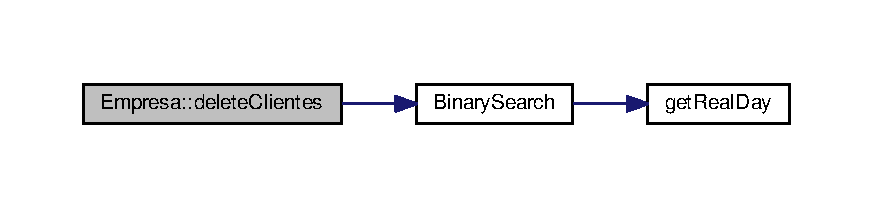
\includegraphics[width=350pt]{classEmpresa_a52b9f4d94c2a05704d74854ed4dd1590_cgraph}
\end{center}
\end{figure}


\index{Empresa@{Empresa}!delete\+Fornecedores@{delete\+Fornecedores}}
\index{delete\+Fornecedores@{delete\+Fornecedores}!Empresa@{Empresa}}
\subsubsection[{\texorpdfstring{delete\+Fornecedores(std\+::string name)}{deleteFornecedores(std::string name)}}]{\setlength{\rightskip}{0pt plus 5cm}{\bf Empresa} \& Empresa\+::delete\+Fornecedores (
\begin{DoxyParamCaption}
\item[{std\+::string}]{name}
\end{DoxyParamCaption}
)}\hypertarget{classEmpresa_ab8b7dda77caceec58e464c16b7e45f7c}{}\label{classEmpresa_ab8b7dda77caceec58e464c16b7e45f7c}


removes a supplier 


\begin{DoxyParams}[1]{Parameters}
\mbox{\tt in}  & {\em name} & The name\\
\hline
\end{DoxyParams}
\begin{DoxyReturn}{Returns}
the modified \hyperlink{classEmpresa}{Empresa} 
\end{DoxyReturn}

\begin{DoxyCode}
67                                                  \{
68 
69     \textcolor{keywordflow}{for} (\textcolor{keywordtype}{unsigned} \textcolor{keywordtype}{int} i = 0; i < \_fornecedores.size(); i++)
70     \{
71         \textcolor{keywordflow}{if} (name == \_fornecedores.at(i)->getNome())
72             \_fornecedores.erase(\_fornecedores.begin() + i);
73     \}
74     \textcolor{keywordflow}{return} *\textcolor{keyword}{this};
75 \}
\end{DoxyCode}
\index{Empresa@{Empresa}!delete\+Reservas@{delete\+Reservas}}
\index{delete\+Reservas@{delete\+Reservas}!Empresa@{Empresa}}
\subsubsection[{\texorpdfstring{delete\+Reservas(std\+::string name)}{deleteReservas(std::string name)}}]{\setlength{\rightskip}{0pt plus 5cm}{\bf Empresa} \& Empresa\+::delete\+Reservas (
\begin{DoxyParamCaption}
\item[{std\+::string}]{name}
\end{DoxyParamCaption}
)}\hypertarget{classEmpresa_a079c008b006f56faac3c1016fe770e8c}{}\label{classEmpresa_a079c008b006f56faac3c1016fe770e8c}


removes a Reservation 


\begin{DoxyParams}[1]{Parameters}
\mbox{\tt in}  & {\em name} & The name\\
\hline
\end{DoxyParams}
\begin{DoxyReturn}{Returns}
the modified \hyperlink{classEmpresa}{Empresa} 
\end{DoxyReturn}

\begin{DoxyCode}
78                                              \{
79 
80     \textcolor{keywordflow}{for} (\textcolor{keywordtype}{unsigned} \textcolor{keywordtype}{int} i = 0; i < \_reservas.size(); i++)
81     \{
82         \textcolor{keywordflow}{if} (name == \_reservas.at(i)->getNomeCliente())
83             \_reservas.erase(\_reservas.begin() + i);
84     \}
85     \textcolor{keywordflow}{return} *\textcolor{keyword}{this};
86 \}
\end{DoxyCode}
\index{Empresa@{Empresa}!desativa\+Cliente@{desativa\+Cliente}}
\index{desativa\+Cliente@{desativa\+Cliente}!Empresa@{Empresa}}
\subsubsection[{\texorpdfstring{desativa\+Cliente(\+Cliente $\ast$c)}{desativaCliente(Cliente *c)}}]{\setlength{\rightskip}{0pt plus 5cm}{\bf Empresa} \& Empresa\+::desativa\+Cliente (
\begin{DoxyParamCaption}
\item[{{\bf Cliente} $\ast$}]{c}
\end{DoxyParamCaption}
)}\hypertarget{classEmpresa_a4c8205b2c4aad43f46172966aaed30b7}{}\label{classEmpresa_a4c8205b2c4aad43f46172966aaed30b7}


Makes a client inactive. 


\begin{DoxyParams}{Parameters}
{\em c} & the client\\
\hline
\end{DoxyParams}
\begin{DoxyReturn}{Returns}
The modified company 
\end{DoxyReturn}

\begin{DoxyCode}
604                                              \{
605     \hyperlink{classClienteInativo}{ClienteInativo} ci(c);
606     this->\_clientesInativos.insert(ci);
607     \textcolor{keywordflow}{return} *\textcolor{keyword}{this};
608 \}
\end{DoxyCode}
\index{Empresa@{Empresa}!display\+Clientes@{display\+Clientes}}
\index{display\+Clientes@{display\+Clientes}!Empresa@{Empresa}}
\subsubsection[{\texorpdfstring{display\+Clientes()}{displayClientes()}}]{\setlength{\rightskip}{0pt plus 5cm}void Empresa\+::display\+Clientes (
\begin{DoxyParamCaption}
{}
\end{DoxyParamCaption}
)}\hypertarget{classEmpresa_a28e04d59daa7206bec6055249ce17410}{}\label{classEmpresa_a28e04d59daa7206bec6055249ce17410}


displays all the information about the Clients 


\begin{DoxyCode}
100 \{
101     \textcolor{keywordflow}{for} (\textcolor{keywordtype}{unsigned} \textcolor{keywordtype}{int} i = 0; i < \_clientes.size(); i++) \{
102         cout << \textcolor{stringliteral}{"Cliente: "} << \_clientes.at(i)->getNome() << endl << \textcolor{stringliteral}{"Morada: "} << \_clientes.at(i)->
      getMorada() << endl << \textcolor{stringliteral}{"Pontos: "} << \_clientes.at(i)->getPontos() << endl;
103         \textcolor{keywordflow}{if} (\_clientes.at(i)->isRegistado()) \{
104             cout << \textcolor{stringliteral}{"Registado: Sim"} << endl << endl;
105         \}
106         \textcolor{keywordflow}{else} cout << \textcolor{stringliteral}{"Registado: Nao"} << endl << endl;
107     \}
108 \}
\end{DoxyCode}
\index{Empresa@{Empresa}!display\+Clientes\+Inativos@{display\+Clientes\+Inativos}}
\index{display\+Clientes\+Inativos@{display\+Clientes\+Inativos}!Empresa@{Empresa}}
\subsubsection[{\texorpdfstring{display\+Clientes\+Inativos()}{displayClientesInativos()}}]{\setlength{\rightskip}{0pt plus 5cm}void Empresa\+::display\+Clientes\+Inativos (
\begin{DoxyParamCaption}
{}
\end{DoxyParamCaption}
)}\hypertarget{classEmpresa_ac7ea4de24979f6623ffe8fbd3d0eeb24}{}\label{classEmpresa_ac7ea4de24979f6623ffe8fbd3d0eeb24}


Lists all the inactive clients. 


\begin{DoxyCode}
635                                      \{
636     tabHInativos::const\_iterator it;
637     \textcolor{keywordflow}{for}(it = this->\_clientesInativos.begin();it != this->\_clientesInativos.end();it++)\{
638         cout << \textcolor{stringliteral}{"Nome: "} <<  it->getNome() << endl << \textcolor{stringliteral}{"Morada: "} << it->getMorada() << endl << endl;
639     \}
640 \}
\end{DoxyCode}
\index{Empresa@{Empresa}!display\+Fornecedores@{display\+Fornecedores}}
\index{display\+Fornecedores@{display\+Fornecedores}!Empresa@{Empresa}}
\subsubsection[{\texorpdfstring{display\+Fornecedores()}{displayFornecedores()}}]{\setlength{\rightskip}{0pt plus 5cm}void Empresa\+::display\+Fornecedores (
\begin{DoxyParamCaption}
{}
\end{DoxyParamCaption}
)}\hypertarget{classEmpresa_a55c3756c01b45b41ad03f4e4f3e4dcac}{}\label{classEmpresa_a55c3756c01b45b41ad03f4e4f3e4dcac}


displays all the information about the suppliers; 


\begin{DoxyCode}
112 \{
113     \textcolor{keywordflow}{for} (\textcolor{keywordtype}{unsigned} \textcolor{keywordtype}{int} i = 0; i < \_fornecedores.size(); i++)
114     \{
115         cout << \textcolor{stringliteral}{"Fornecedor: "} << \_fornecedores.at(i)->getNome() << endl
116             << \textcolor{stringliteral}{"NIF: "} << \_fornecedores.at(i)->getNif() << endl
117             << \textcolor{stringliteral}{"Morada: "} << \_fornecedores.at(i)->getMorada() << endl
118             << \textcolor{stringliteral}{"Definicoes de Fornecedor: "} << endl
119             << \textcolor{stringliteral}{"Preco Base Iate:"} << \_fornecedores.at(i)->getDefinicoesFornecedor().at(1) << endl
120             << \textcolor{stringliteral}{"Preco Base Barco Rebelo:"} << \_fornecedores.at(i)->getDefinicoesFornecedor().at(2) << endl
121             << \textcolor{stringliteral}{"Preco Base Veleiro:"} << \_fornecedores.at(i)->getDefinicoesFornecedor().at(3) << endl
122             << \textcolor{stringliteral}{"Preco por pessoa global:"} << \_fornecedores.at(i)->getDefinicoesFornecedor().at(0) << endl <
      < endl;
123 
124     \}
125 \}
\end{DoxyCode}
\index{Empresa@{Empresa}!display\+Fornecedorescom\+Ofertas@{display\+Fornecedorescom\+Ofertas}}
\index{display\+Fornecedorescom\+Ofertas@{display\+Fornecedorescom\+Ofertas}!Empresa@{Empresa}}
\subsubsection[{\texorpdfstring{display\+Fornecedorescom\+Ofertas()}{displayFornecedorescomOfertas()}}]{\setlength{\rightskip}{0pt plus 5cm}void Empresa\+::display\+Fornecedorescom\+Ofertas (
\begin{DoxyParamCaption}
{}
\end{DoxyParamCaption}
)}\hypertarget{classEmpresa_aa47e9a64800a41180b7f374b73a1f32b}{}\label{classEmpresa_aa47e9a64800a41180b7f374b73a1f32b}


displays all the information about the suppliers all their respective offers 


\begin{DoxyCode}
128 \{
129     \textcolor{keywordflow}{for} (\textcolor{keywordtype}{unsigned} \textcolor{keywordtype}{int} i = 0; i < \_fornecedores.size(); i++)
130     \{
131         cout << \textcolor{stringliteral}{"Fornecedor "} << \_fornecedores.at(i)->getNome() << endl
132             << \textcolor{stringliteral}{"NIF: "} << \_fornecedores.at(i)->getNif() << endl
133             << \textcolor{stringliteral}{"Morada: "} << \_fornecedores.at(i)->getMorada() << endl
134             << \textcolor{stringliteral}{"Definicoes de Fornecedor: "} << endl
135             << \textcolor{stringliteral}{"Preco Base Iate:"} << \_fornecedores.at(i)->getDefinicoesFornecedor().at(1) << endl
136             << \textcolor{stringliteral}{"Preco Base Barco Rebelo:"} << \_fornecedores.at(i)->getDefinicoesFornecedor().at(2) << endl
137             << \textcolor{stringliteral}{"Preco Base Veleiro:"} << \_fornecedores.at(i)->getDefinicoesFornecedor().at(3) << endl
138             << \textcolor{stringliteral}{"Preco por pessoa global:"} << \_fornecedores.at(i)->getDefinicoesFornecedor().at(0) << endl <
      < endl;
139         \_fornecedores.at(i)->displayOfertas();
140         cout << endl;
141 
142 
143     \}
144 \}
\end{DoxyCode}
\index{Empresa@{Empresa}!display\+Ofertasem\+Ordem@{display\+Ofertasem\+Ordem}}
\index{display\+Ofertasem\+Ordem@{display\+Ofertasem\+Ordem}!Empresa@{Empresa}}
\subsubsection[{\texorpdfstring{display\+Ofertasem\+Ordem()}{displayOfertasemOrdem()}}]{\setlength{\rightskip}{0pt plus 5cm}void Empresa\+::display\+Ofertasem\+Ordem (
\begin{DoxyParamCaption}
{}
\end{DoxyParamCaption}
)}\hypertarget{classEmpresa_acd458614a3cca3f432b54212a2e72584}{}\label{classEmpresa_acd458614a3cca3f432b54212a2e72584}


displays all the information about the Offerts without priority order 


\begin{DoxyCode}
567                                     \{
568 
569     \hyperlink{cruise_8h_a50ef8d79980af734cd40fd8d4c2ad566}{pq\_ofertas} temp = queueOfertasOrdenadas;
570 
571 
572     \textcolor{keywordflow}{while} (!(temp.empty())) \{
573         \hyperlink{classOferta}{Oferta} ofertatemp = temp.top();
574 
575         cout << \textcolor{stringliteral}{"Nome: "} << ofertatemp.\hyperlink{classOferta_a16da38d9f369b000cb544c34200707b8}{getNome}() << endl;
576         cout << \textcolor{stringliteral}{"Barco: "} << ofertatemp.\hyperlink{classOferta_aaed9b5937f9f33d2980fcc13ac02132c}{getBarco}() << endl;
577         cout << \textcolor{stringliteral}{"Destinos:"} << endl;
578         \textcolor{keywordflow}{for} (\textcolor{keywordtype}{unsigned} \textcolor{keywordtype}{int} j = 0; j < ofertatemp.\hyperlink{classOferta_a746c91e5db19098d211a3f6bde2ec8ec}{getDestinos}().size(); j++) \{
579 
580             cout << \textcolor{stringliteral}{"Destino numero "} << j + 1 << \textcolor{stringliteral}{" : "} << ofertatemp.
      \hyperlink{classOferta_a746c91e5db19098d211a3f6bde2ec8ec}{getDestinos}().at(j) << endl;
581         \}
582         cout << \textcolor{stringliteral}{"Distancia: "} << ofertatemp.\hyperlink{classOferta_a0d07f80f25f4fb21c0819c3e25d67fb9}{getDistancia}() << endl;
583         cout << \textcolor{stringliteral}{"Lotacao: "} << ofertatemp.\hyperlink{classOferta_a9c8fbec401e54e590828209931bf25b0}{getLotacao}() << endl;
584         cout << \textcolor{stringliteral}{"Data: "} << ofertatemp.\hyperlink{classOferta_a2b156b75371ad59af54ad96ad79c9d1e}{getData}() << endl;
585         cout << \textcolor{stringliteral}{"Preco (por pessoa): "} << ofertatemp.\hyperlink{classOferta_a6237afc2e8a33fb55b1ef0decf9d9aaa}{getPreco}() / ofertatemp.
      \hyperlink{classOferta_a9c8fbec401e54e590828209931bf25b0}{getLotacao}() << endl;
586         cout << \textcolor{stringliteral}{"Preco (total): "} << ofertatemp.\hyperlink{classOferta_a6237afc2e8a33fb55b1ef0decf9d9aaa}{getPreco}() << endl << endl;
587         temp.pop();
588 
589     \}
590 \}
\end{DoxyCode}


Here is the call graph for this function\+:\nopagebreak
\begin{figure}[H]
\begin{center}
\leavevmode
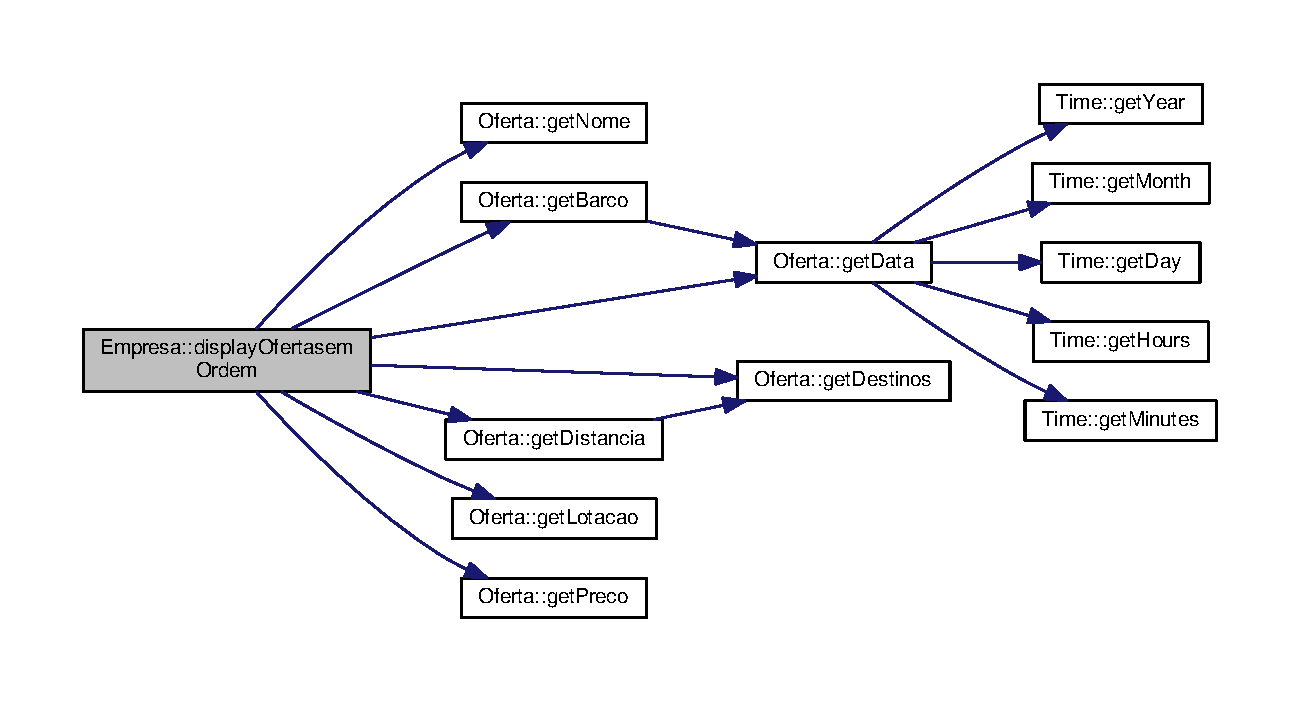
\includegraphics[width=350pt]{classEmpresa_acd458614a3cca3f432b54212a2e72584_cgraph}
\end{center}
\end{figure}


\index{Empresa@{Empresa}!display\+Reservas@{display\+Reservas}}
\index{display\+Reservas@{display\+Reservas}!Empresa@{Empresa}}
\subsubsection[{\texorpdfstring{display\+Reservas()}{displayReservas()}}]{\setlength{\rightskip}{0pt plus 5cm}void Empresa\+::display\+Reservas (
\begin{DoxyParamCaption}
{}
\end{DoxyParamCaption}
)}\hypertarget{classEmpresa_a8c89e6053eaccf0e1938a4f2ab0bfdc4}{}\label{classEmpresa_a8c89e6053eaccf0e1938a4f2ab0bfdc4}


displays all the information about the reservations 


\begin{DoxyCode}
147 \{
148     \textcolor{keywordflow}{for} (\textcolor{keywordtype}{unsigned} \textcolor{keywordtype}{int} i = 0; i < \_reservas.size(); i++)
149     \{
150         cout << \textcolor{stringliteral}{"Fornecedor: "} << \_reservas.at(i)->getNomeFornecedor() << endl
151             << \textcolor{stringliteral}{"Oferta: "};  \_reservas.at(i)->getOferta()->printOferta();
152         cout << \textcolor{stringliteral}{"Cliente: "} << \_reservas.at(i)->getCliente()->getNome() << endl
153             << \textcolor{stringliteral}{"Pontos do Cliente: "} << \_reservas.at(i)->getCliente()->getPontos() << endl
154             << \textcolor{stringliteral}{"Preco (a pagar): "} << \_reservas.at(i)->getPreco() << endl
155             << \textcolor{stringliteral}{"Cancelada: "} << (\_reservas.at(i)->isCancelada()? \textcolor{stringliteral}{"sim"} : \textcolor{stringliteral}{"nao"}) << endl << endl;
156 
157     \}
158 \}
\end{DoxyCode}
\index{Empresa@{Empresa}!display\+Todas\+As\+Ofertasde\+Um\+Fornecedor@{display\+Todas\+As\+Ofertasde\+Um\+Fornecedor}}
\index{display\+Todas\+As\+Ofertasde\+Um\+Fornecedor@{display\+Todas\+As\+Ofertasde\+Um\+Fornecedor}!Empresa@{Empresa}}
\subsubsection[{\texorpdfstring{display\+Todas\+As\+Ofertasde\+Um\+Fornecedor()}{displayTodasAsOfertasdeUmFornecedor()}}]{\setlength{\rightskip}{0pt plus 5cm}void Empresa\+::display\+Todas\+As\+Ofertasde\+Um\+Fornecedor (
\begin{DoxyParamCaption}
{}
\end{DoxyParamCaption}
)}\hypertarget{classEmpresa_a73543b5ca1d9dd8e99e75d9167839471}{}\label{classEmpresa_a73543b5ca1d9dd8e99e75d9167839471}


Lists all the offers of one Supplier. 


\begin{DoxyCode}
770                                                   \{
771 
772     \hyperlink{classEmpresa_ad79f7196a8ce7256771cbd7b9542155c}{titulo}();
773     \textcolor{keywordtype}{string} nome\_fornecedor;
774 
775     \hyperlink{classEmpresa_a55c3756c01b45b41ad03f4e4f3e4dcac}{displayFornecedores}();
776 
777     cout << \textcolor{stringliteral}{"+----------------------------------------------------------+\(\backslash\)n"};
778     cout << \textcolor{stringliteral}{"| Qual e o nome do fornecedor?                                |\(\backslash\)n"};
779     cout << \textcolor{stringliteral}{"+----------------------------------------------------------+\(\backslash\)n"};
780 
781     cin.ignore(INT\_MAX, \textcolor{charliteral}{'\(\backslash\)n'});
782     getline(cin, nome\_fornecedor);
783 
784 
785     \textcolor{keywordtype}{int} index = \hyperlink{extras_8h_abc85c93edf561168b5bbee8054caa388}{BinarySearch}(\_fornecedores, nome\_fornecedor);
786     \textcolor{keywordflow}{if} (index == -1) \{ \textcolor{keywordflow}{throw} \hyperlink{classObjetoInexistente}{ObjetoInexistente<Fornecedor>}(nome\_fornecedor); \}
787     cout << \textcolor{stringliteral}{"+----------------------------------------------------------+\(\backslash\)n"};
788     cout << \textcolor{stringliteral}{"| Estas são todas as reservas efetuadas pelo fornecedor:      |\(\backslash\)n"};
789     cout << \textcolor{stringliteral}{"+----------------------------------------------------------+\(\backslash\)n"};
790 
791     \_fornecedores[index]->displayOfertas();
792 
793     \textcolor{keywordflow}{return};
794 
795 
796 \}
\end{DoxyCode}


Here is the call graph for this function\+:\nopagebreak
\begin{figure}[H]
\begin{center}
\leavevmode
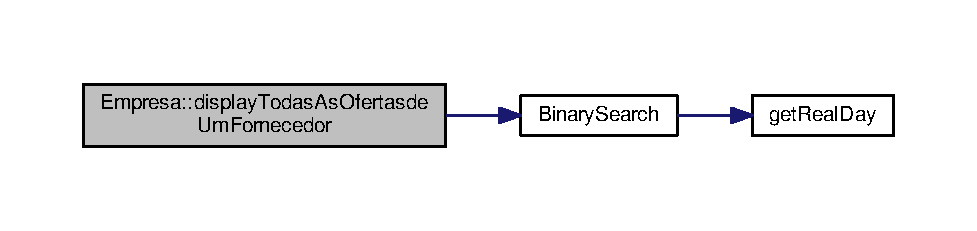
\includegraphics[width=350pt]{classEmpresa_a73543b5ca1d9dd8e99e75d9167839471_cgraph}
\end{center}
\end{figure}


\index{Empresa@{Empresa}!display\+Todas\+As\+Reservasde\+Um\+Cliente@{display\+Todas\+As\+Reservasde\+Um\+Cliente}}
\index{display\+Todas\+As\+Reservasde\+Um\+Cliente@{display\+Todas\+As\+Reservasde\+Um\+Cliente}!Empresa@{Empresa}}
\subsubsection[{\texorpdfstring{display\+Todas\+As\+Reservasde\+Um\+Cliente()}{displayTodasAsReservasdeUmCliente()}}]{\setlength{\rightskip}{0pt plus 5cm}void Empresa\+::display\+Todas\+As\+Reservasde\+Um\+Cliente (
\begin{DoxyParamCaption}
{}
\end{DoxyParamCaption}
)}\hypertarget{classEmpresa_a259bb6b172011429c6e24feb0285e66b}{}\label{classEmpresa_a259bb6b172011429c6e24feb0285e66b}


Lists all the reservations made by one client. 


\begin{DoxyCode}
365                                                 \{
366 
367     \hyperlink{classEmpresa_ad79f7196a8ce7256771cbd7b9542155c}{titulo}();
368     \textcolor{keywordtype}{string} nome\_cliente;
369 
370     \hyperlink{classEmpresa_a28e04d59daa7206bec6055249ce17410}{displayClientes}();
371 
372     cout << \textcolor{stringliteral}{"+----------------------------------------------------------+\(\backslash\)n"};
373     cout << \textcolor{stringliteral}{"| Qual e o nome do cliente?                                |\(\backslash\)n"};
374     cout << \textcolor{stringliteral}{"+----------------------------------------------------------+\(\backslash\)n"};
375 
376     cin.ignore(INT\_MAX, \textcolor{charliteral}{'\(\backslash\)n'});
377     getline(cin, nome\_cliente);
378 
379 
380     \textcolor{keywordtype}{int} index = \hyperlink{extras_8h_abc85c93edf561168b5bbee8054caa388}{BinarySearch}(\_clientes, nome\_cliente);
381     \textcolor{keywordflow}{if} (index == -1) \{ \textcolor{keywordflow}{throw} \hyperlink{classObjetoInexistente}{ObjetoInexistente<Cliente>}(nome\_cliente); \}
382     cout << \textcolor{stringliteral}{"+----------------------------------------------------------+\(\backslash\)n"};
383     cout << \textcolor{stringliteral}{"| Estas são todas as reservas efetuadas pelo cliente:      |\(\backslash\)n"};
384     cout << \textcolor{stringliteral}{"+----------------------------------------------------------+\(\backslash\)n"};
385 
386     \textcolor{keywordflow}{for} (\textcolor{keywordtype}{unsigned} \textcolor{keywordtype}{int} i = 0; i < \_reservas.size(); i++)
387     \{
388         \textcolor{keywordflow}{if} (\_reservas[i]->getNomeCliente() == nome\_cliente)
389         \{
390             cout << \textcolor{stringliteral}{"Fornecedor: "} << \_reservas.at(i)->getNomeFornecedor() << endl
391                 << \textcolor{stringliteral}{"Oferta: "};  \_reservas.at(i)->getOferta()->printOferta();
392             cout << \textcolor{stringliteral}{"Cliente: "} << \_reservas.at(i)->getCliente()->getNome() << endl
393                 << \textcolor{stringliteral}{"Pontos do Cliente: "} << \_reservas.at(i)->getCliente()->getPontos() << endl
394                 << \textcolor{stringliteral}{"Preco (a pagar): "} << \_reservas.at(i)->getPreco() << endl
395                 << \textcolor{stringliteral}{"Cancelada: "} << (\_reservas.at(i)->isCancelada() ? \textcolor{stringliteral}{"sim"} : \textcolor{stringliteral}{"nao"}) << endl << endl;
396         \}
397     \}
398 
399 
400 \}
\end{DoxyCode}


Here is the call graph for this function\+:\nopagebreak
\begin{figure}[H]
\begin{center}
\leavevmode
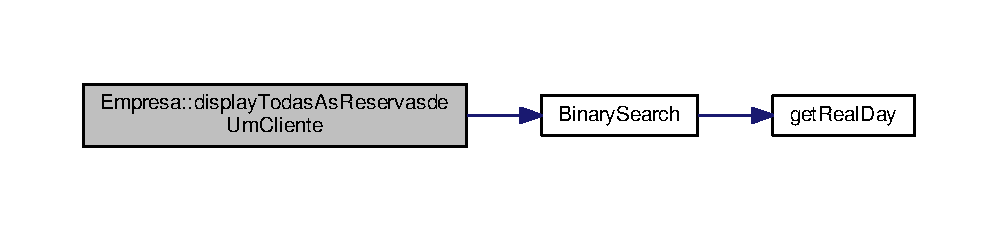
\includegraphics[width=350pt]{classEmpresa_a259bb6b172011429c6e24feb0285e66b_cgraph}
\end{center}
\end{figure}


\index{Empresa@{Empresa}!display\+Todas\+As\+Reservasde\+Um\+Fornecedor@{display\+Todas\+As\+Reservasde\+Um\+Fornecedor}}
\index{display\+Todas\+As\+Reservasde\+Um\+Fornecedor@{display\+Todas\+As\+Reservasde\+Um\+Fornecedor}!Empresa@{Empresa}}
\subsubsection[{\texorpdfstring{display\+Todas\+As\+Reservasde\+Um\+Fornecedor()}{displayTodasAsReservasdeUmFornecedor()}}]{\setlength{\rightskip}{0pt plus 5cm}void Empresa\+::display\+Todas\+As\+Reservasde\+Um\+Fornecedor (
\begin{DoxyParamCaption}
{}
\end{DoxyParamCaption}
)}\hypertarget{classEmpresa_af197726a3dc20739aac877ac4c090f6e}{}\label{classEmpresa_af197726a3dc20739aac877ac4c090f6e}


Lists all the reservations with offers of one supplier. 


\begin{DoxyCode}
720                                                    \{
721 
722     \hyperlink{classEmpresa_ad79f7196a8ce7256771cbd7b9542155c}{titulo}();
723     \textcolor{keywordtype}{string} nome\_fornecedor;
724     \textcolor{keywordtype}{bool} existe = \textcolor{keyword}{false};
725 
726     \hyperlink{classEmpresa_a55c3756c01b45b41ad03f4e4f3e4dcac}{displayFornecedores}();
727 
728     cout << \textcolor{stringliteral}{"+----------------------------------------------------------+\(\backslash\)n"};
729     cout << \textcolor{stringliteral}{"| Qual e o nome do fornecedor?                                |\(\backslash\)n"};
730     cout << \textcolor{stringliteral}{"+----------------------------------------------------------+\(\backslash\)n"};
731 
732     cin.ignore(INT\_MAX, \textcolor{charliteral}{'\(\backslash\)n'});
733     getline(cin, nome\_fornecedor);
734 
735 
736     \textcolor{keywordtype}{int} index = \hyperlink{extras_8h_abc85c93edf561168b5bbee8054caa388}{BinarySearch}(\_fornecedores, nome\_fornecedor);
737     \textcolor{keywordflow}{if} (index == -1) \{ \textcolor{keywordflow}{throw} \hyperlink{classObjetoInexistente}{ObjetoInexistente<Fornecedor>}(nome\_fornecedor); \}
738     cout << \textcolor{stringliteral}{"+----------------------------------------------------------+\(\backslash\)n"};
739     cout << \textcolor{stringliteral}{"| Estas são as reservas efetuadas para este fornecedor:    |\(\backslash\)n"};
740     cout << \textcolor{stringliteral}{"+----------------------------------------------------------+\(\backslash\)n"};
741 
742     \textcolor{keywordflow}{for} (\textcolor{keywordtype}{unsigned} \textcolor{keywordtype}{int} i = 0; i < \_reservas.size(); i++)
743     \{
744         \textcolor{keywordflow}{if} (\_reservas[i]->getNomeFornecedor() == nome\_fornecedor)
745         \{
746             existe = \textcolor{keyword}{true};
747 
748             cout << \textcolor{stringliteral}{"Fornecedor: "} << \_reservas.at(i)->getNomeFornecedor() << endl
749                 << \textcolor{stringliteral}{"Oferta: "};  \_reservas.at(i)->getOferta()->printOferta();
750             cout << \textcolor{stringliteral}{"Cliente: "} << \_reservas.at(i)->getCliente()->getNome() << endl
751                 << \textcolor{stringliteral}{"Pontos do Cliente: "} << \_reservas.at(i)->getCliente()->getPontos() << endl
752                 << \textcolor{stringliteral}{"Preco (a pagar): "} << \_reservas.at(i)->getPreco() << endl
753                 << \textcolor{stringliteral}{"Cancelada: "} << (\_reservas.at(i)->isCancelada() ? \textcolor{stringliteral}{"sim"} : \textcolor{stringliteral}{"nao"}) << endl << endl;
754         \}
755         
756     \}
757     \textcolor{keywordflow}{if} (!existe)
758     \{
759         cout << \textcolor{stringliteral}{"+----------------------------------------------------------+\(\backslash\)n"};
760         cout << \textcolor{stringliteral}{"| Ninguem reservou uma oferta deste fornecedor!            |\(\backslash\)n"};
761         cout << \textcolor{stringliteral}{"+----------------------------------------------------------+\(\backslash\)n"};
762     \}
763 
764     \textcolor{keywordflow}{return};
765 
766 
767 \}
\end{DoxyCode}


Here is the call graph for this function\+:\nopagebreak
\begin{figure}[H]
\begin{center}
\leavevmode
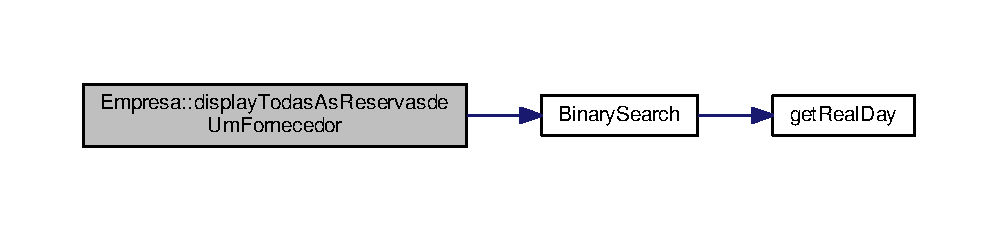
\includegraphics[width=350pt]{classEmpresa_af197726a3dc20739aac877ac4c090f6e_cgraph}
\end{center}
\end{figure}


\index{Empresa@{Empresa}!display\+Todos\+Os\+Clientesdeuma\+Oferta@{display\+Todos\+Os\+Clientesdeuma\+Oferta}}
\index{display\+Todos\+Os\+Clientesdeuma\+Oferta@{display\+Todos\+Os\+Clientesdeuma\+Oferta}!Empresa@{Empresa}}
\subsubsection[{\texorpdfstring{display\+Todos\+Os\+Clientesdeuma\+Oferta()}{displayTodosOsClientesdeumaOferta()}}]{\setlength{\rightskip}{0pt plus 5cm}void Empresa\+::display\+Todos\+Os\+Clientesdeuma\+Oferta (
\begin{DoxyParamCaption}
{}
\end{DoxyParamCaption}
)}\hypertarget{classEmpresa_a641c2eb827b39ab79919187645ff71a9}{}\label{classEmpresa_a641c2eb827b39ab79919187645ff71a9}


Lists all the clients that reserved a certain offer. 


\begin{DoxyCode}
1390                                                 \{
1391     
1392     \hyperlink{classEmpresa_aa47e9a64800a41180b7f374b73a1f32b}{displayFornecedorescomOfertas}();
1393     \textcolor{keywordtype}{string} nomeOferta,nomefornecedor;
1394     \textcolor{keywordtype}{int} index, indexOferta;
1395     \textcolor{keywordtype}{bool} nfound = \textcolor{keyword}{true};
1396 
1397     cout << \textcolor{stringliteral}{"+----------------------------------------------------------+\(\backslash\)n"};
1398     cout << \textcolor{stringliteral}{"| Indique o fornecedor em questão:                         |\(\backslash\)n"};
1399     cout << \textcolor{stringliteral}{"+----------------------------------------------------------+\(\backslash\)n"};
1400 
1401 
1402     cin.ignore(INT\_MAX, \textcolor{charliteral}{'\(\backslash\)n'});
1403     getline(cin, nomefornecedor);
1404     index = \hyperlink{extras_8h_abc85c93edf561168b5bbee8054caa388}{BinarySearch}(this->\_fornecedores, nomefornecedor);
1405     \textcolor{keywordflow}{if} (index == -1) \{
1406         \textcolor{keywordflow}{throw} \hyperlink{classObjetoInexistente}{ObjetoInexistente<Fornecedor>}(nomefornecedor);
1407     \}
1408 
1409 
1410     
1411 
1412     cout << \textcolor{stringliteral}{"+----------------------------------------------------------+\(\backslash\)n"};
1413     cout << \textcolor{stringliteral}{"| Indique o nome da oferta em questao:                     |\(\backslash\)n"};
1414     cout << \textcolor{stringliteral}{"+----------------------------------------------------------+\(\backslash\)n"};
1415 
1416     getline(cin, nomeOferta);
1417 
1418     indexOferta = -1;
1419     \textcolor{keywordflow}{for} (\textcolor{keywordtype}{unsigned} \textcolor{keywordtype}{int} i = 0; i <\_fornecedores.at(index)->getOfertas().size(); i++)
1420     \{
1421 
1422         \textcolor{keywordflow}{if} (\_fornecedores.at(index)->getOfertas().at(i).getNome() == nomeOferta)
1423         \{
1424             indexOferta = i;
1425         \}
1426     \}
1427     \textcolor{keywordflow}{if} (indexOferta == -1) \{ \textcolor{keywordflow}{throw} \hyperlink{classObjetoInexistente}{ObjetoInexistente<Oferta>}(nomeOferta); \}
1428 
1429     \textcolor{keywordflow}{for} (\textcolor{keywordtype}{unsigned} \textcolor{keywordtype}{int} j = 0; j < \_reservas.size(); j++)
1430     \{
1431         \textcolor{keywordflow}{if} (\_reservas.at(j)->getOferta()->getNome() == nomeOferta)
1432         \{
1433 
1434             nfound = \textcolor{keyword}{false};
1435 
1436             \textcolor{keywordflow}{for} (\textcolor{keywordtype}{unsigned} \textcolor{keywordtype}{int} i = 0; i < \_clientes.size(); i++)
1437             \{
1438                 \textcolor{keywordflow}{if} (\_reservas.at(j)->getNomeCliente() == \_clientes.at(i)->getNome())
1439                 \{
1440                     cout << \textcolor{stringliteral}{"Cliente: "} << \_clientes.at(i)->getNome() << endl << \textcolor{stringliteral}{"Morada: "} << \_clientes.at
      (i)->getMorada() << endl << \textcolor{stringliteral}{"Pontos: "} << \_clientes.at(i)->getPontos() << endl;
1441                     \textcolor{keywordflow}{if} (\_clientes.at(i)->isRegistado()) \{
1442                         cout << \textcolor{stringliteral}{"Registado: Sim"} << endl << endl;
1443                     \}
1444                     \textcolor{keywordflow}{else} cout << \textcolor{stringliteral}{"Registado: Nao"} << endl << endl;
1445                 \}
1446             \}
1447         \}
1448     \}
1449     \textcolor{keywordflow}{if} (nfound) \{
1450         \textcolor{keywordflow}{throw} \hyperlink{classObjetoInexistente}{ObjetoInexistente<Reserva>}(\textcolor{stringliteral}{""});
1451     \}
1452 
1453 
1454 
1455 \}
\end{DoxyCode}


Here is the call graph for this function\+:\nopagebreak
\begin{figure}[H]
\begin{center}
\leavevmode
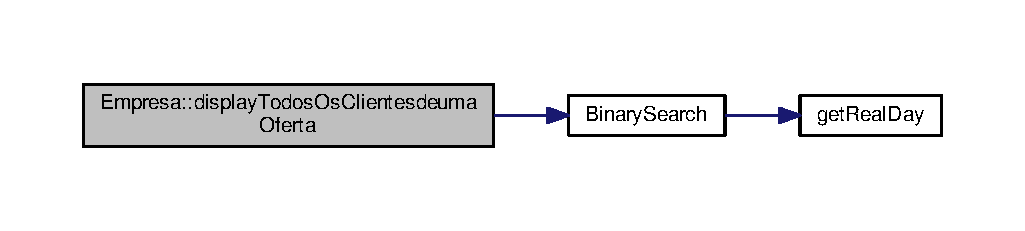
\includegraphics[width=350pt]{classEmpresa_a641c2eb827b39ab79919187645ff71a9_cgraph}
\end{center}
\end{figure}


\index{Empresa@{Empresa}!get\+Clientes@{get\+Clientes}}
\index{get\+Clientes@{get\+Clientes}!Empresa@{Empresa}}
\subsubsection[{\texorpdfstring{get\+Clientes()}{getClientes()}}]{\setlength{\rightskip}{0pt plus 5cm}const std\+::vector$<$ {\bf Cliente} $\ast$ $>$ \& Empresa\+::get\+Clientes (
\begin{DoxyParamCaption}
{}
\end{DoxyParamCaption}
)}\hypertarget{classEmpresa_a472beae89ee1187e1ec3f70e9d4a99ef}{}\label{classEmpresa_a472beae89ee1187e1ec3f70e9d4a99ef}


Gets the clients. 

\begin{DoxyReturn}{Returns}
The clientes. 
\end{DoxyReturn}

\begin{DoxyCode}
34                                                 \{
35     \textcolor{keywordflow}{return} this->\_clientes;
36 \}
\end{DoxyCode}
\index{Empresa@{Empresa}!get\+Fornecedores@{get\+Fornecedores}}
\index{get\+Fornecedores@{get\+Fornecedores}!Empresa@{Empresa}}
\subsubsection[{\texorpdfstring{get\+Fornecedores()}{getFornecedores()}}]{\setlength{\rightskip}{0pt plus 5cm}const std\+::vector$<$ {\bf Fornecedor} $\ast$ $>$ \& Empresa\+::get\+Fornecedores (
\begin{DoxyParamCaption}
{}
\end{DoxyParamCaption}
)}\hypertarget{classEmpresa_aaf131a375aa70819205744328a4dbc07}{}\label{classEmpresa_aaf131a375aa70819205744328a4dbc07}


Gets the suppliers. 

\begin{DoxyReturn}{Returns}
The fornecedores. 
\end{DoxyReturn}

\begin{DoxyCode}
30                                                        \{
31     \textcolor{keywordflow}{return} this->\_fornecedores;
32 \}
\end{DoxyCode}
\index{Empresa@{Empresa}!lista\+Faturas@{lista\+Faturas}}
\index{lista\+Faturas@{lista\+Faturas}!Empresa@{Empresa}}
\subsubsection[{\texorpdfstring{lista\+Faturas()}{listaFaturas()}}]{\setlength{\rightskip}{0pt plus 5cm}void Empresa\+::lista\+Faturas (
\begin{DoxyParamCaption}
{}
\end{DoxyParamCaption}
)}\hypertarget{classEmpresa_ab1950b5b5e9fca80823b5d01c6c1de6f}{}\label{classEmpresa_ab1950b5b5e9fca80823b5d01c6c1de6f}


Lists all the bills. 


\begin{DoxyCode}
161                            \{
162 
163     \hyperlink{classBSTItrIn}{BSTItrIn<Fatura>} it(\_faturas);
164     \textcolor{keywordflow}{while} (!it.isAtEnd()) \{
165 
166 
167         cout << \textcolor{stringliteral}{"----------------------------------------------------\(\backslash\)n"} << endl;
168 
169         cout << \textcolor{stringliteral}{"Nome do cliente: "} << it.retrieve().getNomeCliente() << endl;
170         cout << \textcolor{stringliteral}{"Fornecedor: "} << it.retrieve().getFornecedor() << endl;
171         cout << \textcolor{stringliteral}{"Data de faturacao: "};
172         it.retrieve().getData().printTime(cout);
173         cout << endl;
174         it.advance();
175     \}
176 
177     
178 \}
\end{DoxyCode}


Here is the call graph for this function\+:\nopagebreak
\begin{figure}[H]
\begin{center}
\leavevmode
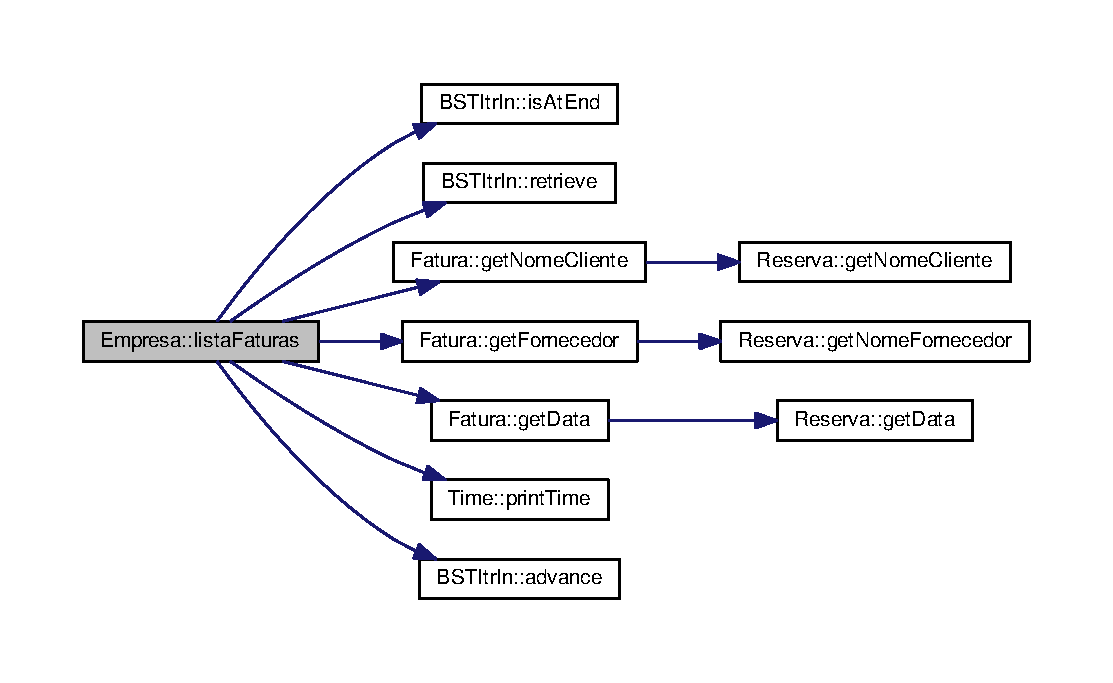
\includegraphics[width=350pt]{classEmpresa_ab1950b5b5e9fca80823b5d01c6c1de6f_cgraph}
\end{center}
\end{figure}


\index{Empresa@{Empresa}!load@{load}}
\index{load@{load}!Empresa@{Empresa}}
\subsubsection[{\texorpdfstring{load()}{load()}}]{\setlength{\rightskip}{0pt plus 5cm}void Empresa\+::load (
\begin{DoxyParamCaption}
{}
\end{DoxyParamCaption}
)}\hypertarget{classEmpresa_a3445c3c507b4f45d1d7831908ff4cdf1}{}\label{classEmpresa_a3445c3c507b4f45d1d7831908ff4cdf1}


loads the information generated in previous executions 


\begin{DoxyCode}
180                   \{
181     ifstream clientes\_file(\textcolor{stringliteral}{"clientes.txt"});
182     ifstream registados\_file(\textcolor{stringliteral}{"clientes\_registados.txt"});
183     ifstream fornecedores\_file(\textcolor{stringliteral}{"fornecedores.txt"});
184     ifstream reservas\_file(\textcolor{stringliteral}{"reservas.txt"});
185     \textcolor{keywordtype}{string} line;
186     \textcolor{keywordtype}{string} s1;
187     \textcolor{keywordtype}{string} s2;
188     \textcolor{keywordtype}{string} s3;
189     \textcolor{keywordtype}{string} morada;
190     \textcolor{keywordtype}{unsigned} \textcolor{keywordtype}{int} num1;
191     \textcolor{keywordtype}{unsigned} \textcolor{keywordtype}{int} num2;
192     vector<int> v;
193     \textcolor{keywordtype}{unsigned} \textcolor{keywordtype}{int} p;
194     vector<string> destinos;
195     \hyperlink{classCliente}{Cliente} * c = NULL;
196     \hyperlink{classFornecedor}{Fornecedor} * f;
197     \hyperlink{classOferta}{Oferta} * o = NULL;
198     \hyperlink{classReserva}{Reserva} * r;
199     \hyperlink{classTime}{Time} * t;
200     \hyperlink{classTime}{Time} * t2;
201     vector<Oferta> ofertas;
202     \textcolor{comment}{//Stores the clients who aren't registered in the data base}
203     \textcolor{keywordflow}{if}(clientes\_file.is\_open())
204         \textcolor{keywordflow}{while}(getline(clientes\_file,line))\{
205             s1 = line;
206             getline(clientes\_file,line);
207             s2 = line;
208             c = \textcolor{keyword}{new} \hyperlink{classCliente}{Cliente}(s1,s2);
209             this->\hyperlink{classEmpresa_a57597ec4154f274686bc648ccf5d2a59}{addClientes}(*c);
210         \}
211     \textcolor{keywordflow}{else} \{
212         cout << \textcolor{stringliteral}{"O programa falhou a abrir o ficheiro com a informacao de clientes"} << endl;
213     \}
214     clientes\_file.close();
215     \textcolor{comment}{//Stores the clients who are registered in the data base}
216     s1.clear();
217     s2.clear();
218     \textcolor{keywordflow}{if}(registados\_file.is\_open())
219             \textcolor{keywordflow}{while}(getline(registados\_file,line))\{
220                 s1 = line;
221                 getline(registados\_file,line);
222                 s2 = line;
223                 getline(registados\_file,line,\textcolor{charliteral}{'\(\backslash\)n'});
224                 num1 = stoi(line);
225                 c = \textcolor{keyword}{new} \hyperlink{classClienteRegistado}{ClienteRegistado}(s1,s2,num1);
226                 this->\hyperlink{classEmpresa_a57597ec4154f274686bc648ccf5d2a59}{addClientes}(*c);
227             \}
228         \textcolor{keywordflow}{else} \{
229             cout << \textcolor{stringliteral}{"O programa falhou a abrir o ficheiro com a informacao de clientes registados"} << endl;
230         \}
231     registados\_file.close();
232    \textcolor{comment}{//Stores the supplier}
233     \textcolor{keywordflow}{if}(fornecedores\_file.is\_open())\{
234             \textcolor{keywordflow}{while}(getline(fornecedores\_file,line))\{
235                 s1 = line;
236                 getline(fornecedores\_file,line,\textcolor{charliteral}{'\(\backslash\)n'});
237                 num1 = stoi(line);
238                 getline(fornecedores\_file,line);
239                 s2 = line;
240                 f = \textcolor{keyword}{new} \hyperlink{classFornecedor}{Fornecedor}(s1,num1,s2);
241                 getline(fornecedores\_file,line);
242                 v.push\_back(stoi(line));
243                 getline(fornecedores\_file,line);
244                 v.push\_back(stoi(line));
245                 getline(fornecedores\_file,line);
246                 v.push\_back(stoi(line));
247                 getline(fornecedores\_file,line);
248                 v.push\_back(stoi(line));
249                 f->\hyperlink{classFornecedor_a63bb5795c45d195995de437620503d98}{setDefenicoes}(v);
250                 v.clear();
251                 \textcolor{keywordflow}{while}(\textcolor{keyword}{true})\{
252                     getline(fornecedores\_file,line);
253                     \textcolor{keywordflow}{if}(line == \textcolor{stringliteral}{"fend"})
254                         \textcolor{keywordflow}{break};
255                     \textcolor{keywordflow}{else}\{
256                         s1 = line;
257                         getline(fornecedores\_file,line);
258                         s2 = line;
259                         getline(fornecedores\_file,line,\textcolor{charliteral}{'\(\backslash\)n'});
260                         num1 = stoi(line);
261                         getline(fornecedores\_file,line,\textcolor{charliteral}{'\(\backslash\)n'});
262                         num2 = stoi(line);
263                         getline(fornecedores\_file,line);
264                         t = \textcolor{keyword}{new} \hyperlink{classTime}{Time}(line);
265                         getline(fornecedores\_file,line);
266                         t2 = \textcolor{keyword}{new} \hyperlink{classTime}{Time}(line);
267                         getline(fornecedores\_file,line,\textcolor{charliteral}{'\(\backslash\)n'});
268 
269                         p = stoi(line);
270                         getline(fornecedores\_file,line);
271                         \textcolor{keywordflow}{if}(line == \textcolor{stringliteral}{"oend"})\{
272                             \textcolor{keywordflow}{break};
273                         \}
274                         \textcolor{keywordflow}{else}\{
275                             \textcolor{keywordflow}{do}\{
276                                 destinos.push\_back(line);
277                                 getline(fornecedores\_file,line);
278                             \} \textcolor{keywordflow}{while}(line != \textcolor{stringliteral}{"oend"});
279                         \}
280                         o = \textcolor{keyword}{new} \hyperlink{classOferta}{Oferta}(s1,s2,destinos,num1,num2,*t,p);
281                         o->\hyperlink{classOferta_a50c041d2301a351f2ac69ed235175116}{setTimeUltimaReserva}(*t2);
282                         f->\hyperlink{classFornecedor_a220373fd19f44a30d7c6c1ec913be700}{addOferta}(*o);
283 
284 
285                     \}
286                 \}
287 
288                 this->\hyperlink{classEmpresa_a0c858479d6e92094adbb2fc085039376}{addFornecedores}(*f);
289             \}
290     \}
291         \textcolor{keywordflow}{else} \{
292             cout << \textcolor{stringliteral}{"O programa falhou a abrir o ficheiro com a informacao de fornecedores"} << endl;
293         \}
294     fornecedores\_file.close();
295 
296     \textcolor{keywordtype}{bool} cancelada;
297     \textcolor{keywordflow}{if}(reservas\_file.is\_open())\{
298         \textcolor{keywordflow}{while}(getline(reservas\_file,line))\{
299             s1 = line;
300             getline(reservas\_file,line);
301             s2 = line;
302             getline(reservas\_file,line);
303             \textcolor{keywordflow}{if}(line == \textcolor{stringliteral}{"true"})\{
304                 cancelada = \textcolor{keyword}{true};
305             \}
306             \textcolor{keywordflow}{else} cancelada = \textcolor{keyword}{false};
307             getline(reservas\_file,line, \textcolor{charliteral}{'\(\backslash\)n'});
308 
309             num1 = stoi(line);
310             \textcolor{keywordflow}{for}(\textcolor{keywordtype}{unsigned} \textcolor{keywordtype}{int} i = 0; i < this->\_clientes.size();i++)\{
311                 \textcolor{keywordflow}{if}(this->\_clientes[i]->getNome() == s2)\{
312                     *c = *this->\_clientes[i];
313                 \}
314             \}
315             \textcolor{keywordflow}{for}(\textcolor{keywordtype}{unsigned} \textcolor{keywordtype}{int} i = 0; i < this->\_fornecedores.size();i++)\{
316                             \textcolor{keywordflow}{for}(\textcolor{keywordtype}{unsigned} \textcolor{keywordtype}{int} j = 0;j < this->\_fornecedores[i]->getOfertas().size();j++)\{
317                                 \textcolor{keywordflow}{if}(this->\_fornecedores[i]->getOfertas().at(j).getNome() == s1)\{
318                                     *o = this->\_fornecedores[i]->getOfertas()[j];
319                                 \}
320                             \}
321                         \}
322             r = \textcolor{keyword}{new} \hyperlink{classReserva}{Reserva}(s1,o,s2,c,num1,cancelada);
323             this->\hyperlink{classEmpresa_a42a1671b234ab8380cfb2ed33517edb2}{addReservas}(*r);
324         \}
325     \}
326     \textcolor{keywordflow}{else}\{
327         cout << \textcolor{stringliteral}{"Erro: O programa nao conseguiu abrir o ficheiro das reservas"} << endl;
328     \}
329     this->\hyperlink{classEmpresa_aa7424cde3bdf1b1921967bc176d0ab50}{sort}();
330 
331 
332     reservas\_file.close();
333 \}
\end{DoxyCode}


Here is the call graph for this function\+:
\nopagebreak
\begin{figure}[H]
\begin{center}
\leavevmode
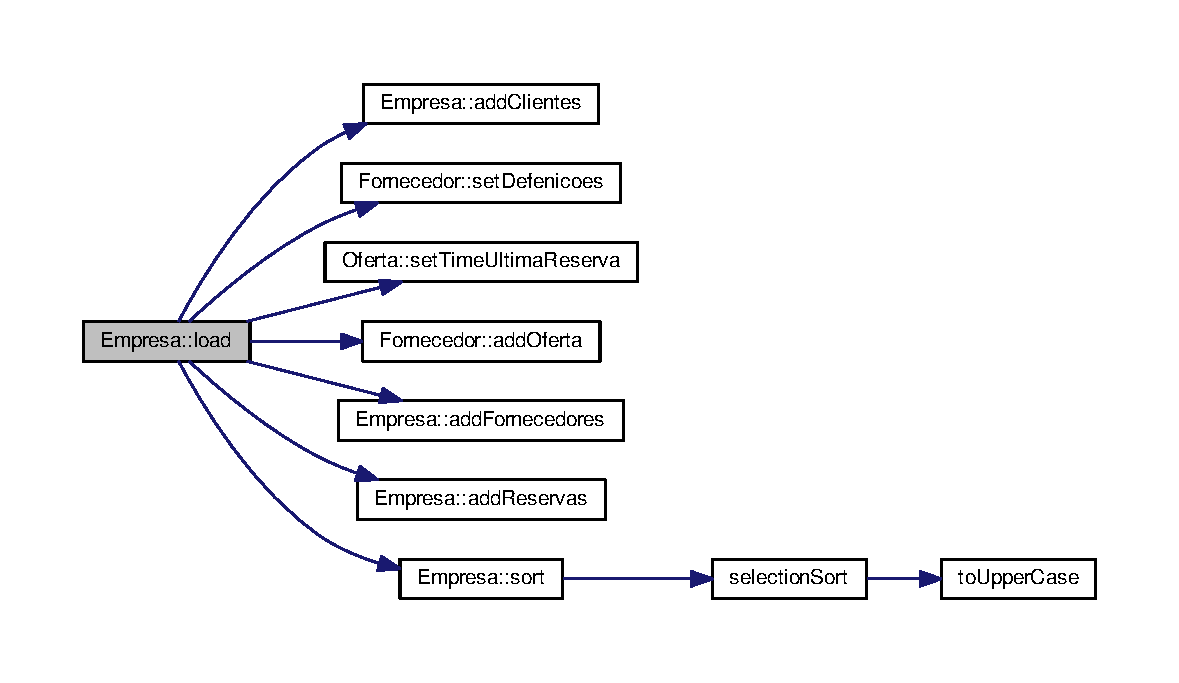
\includegraphics[width=350pt]{classEmpresa_a3445c3c507b4f45d1d7831908ff4cdf1_cgraph}
\end{center}
\end{figure}




Here is the caller graph for this function\+:\nopagebreak
\begin{figure}[H]
\begin{center}
\leavevmode
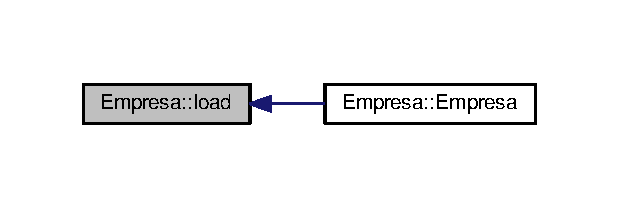
\includegraphics[width=297pt]{classEmpresa_a3445c3c507b4f45d1d7831908ff4cdf1_icgraph}
\end{center}
\end{figure}


\index{Empresa@{Empresa}!menu\+Cliente@{menu\+Cliente}}
\index{menu\+Cliente@{menu\+Cliente}!Empresa@{Empresa}}
\subsubsection[{\texorpdfstring{menu\+Cliente()}{menuCliente()}}]{\setlength{\rightskip}{0pt plus 5cm}void Empresa\+::menu\+Cliente (
\begin{DoxyParamCaption}
{}
\end{DoxyParamCaption}
)}\hypertarget{classEmpresa_a2e8e13ecd162403da0118ceccdccbbcb}{}\label{classEmpresa_a2e8e13ecd162403da0118ceccdccbbcb}


displays the Client Menu 

displays the client menu 
\begin{DoxyCode}
32                           \{
33 
34 
35     \textcolor{keywordtype}{int} opcaocliente;
36     \textcolor{keywordflow}{while} (\textcolor{keyword}{true}) \{
37         \hyperlink{classEmpresa_ad79f7196a8ce7256771cbd7b9542155c}{titulo}();
38         cout << \textcolor{stringliteral}{"+----------------------------------------------------------+\(\backslash\)n"};
39         cout << \textcolor{stringliteral}{"| Escolha o que pretende fazer com os clientes             |\(\backslash\)n"};
40         cout << \textcolor{stringliteral}{"+----------------------------------------------------------+\(\backslash\)n"};
41         cout << \textcolor{stringliteral}{"| Selecione a sua opcao (insira apenas o numero):          |\(\backslash\)n"};
42         cout << \textcolor{stringliteral}{"+----------------------------------------------------------+ \(\backslash\)n"};
43         cout << \textcolor{stringliteral}{"| 1 - Adicionar Cliente                                    |\(\backslash\)n"};
44         cout << \textcolor{stringliteral}{"| 2 - Modificar Cliente                                    |\(\backslash\)n"};
45         cout << \textcolor{stringliteral}{"| 3 - Apagar Cliente                                       |\(\backslash\)n"};
46         cout << \textcolor{stringliteral}{"| 4 - Ver Todos os Clientes                                |\(\backslash\)n"};
47         cout << \textcolor{stringliteral}{"| 5 - Ver Todos os Clientes Inativos                       |\(\backslash\)n"};
48         cout << \textcolor{stringliteral}{"| 6 - Ver Faturas                                          |\(\backslash\)n"};
49         cout << \textcolor{stringliteral}{"| 7 - Ver Todas as Reservas de um Cliente                  |\(\backslash\)n"};
50         cout << \textcolor{stringliteral}{"| 0 - Sair                                                 |\(\backslash\)n"};
51         cout << \textcolor{stringliteral}{"+----------------------------------------------------------+\(\backslash\)n"};
52 
53         cin >> opcaocliente;
54 
55         \textcolor{keywordflow}{if} (cin.fail())\{
56             cin.clear();
57             cin.ignore(INT\_MAX,\textcolor{charliteral}{'\(\backslash\)n'});
58             \hyperlink{menu_8h_aceb70c1ed7e11f0863a868704f02214b}{clearScreen}();
59             cout << \textcolor{stringliteral}{"Erro: Introduziu um input invalido. So pode usar numeros inteiros."} << endl;
60             cout << \textcolor{stringliteral}{"Pressione Enter para voltar ao menu"} << endl;
61             cin.get();
62         \}
63         \textcolor{keywordflow}{switch} (opcaocliente) \{
64 
65         \textcolor{keywordflow}{case} 0:
66             \textcolor{keywordflow}{return};
67             \textcolor{keywordflow}{break};
68 
69         \textcolor{keywordflow}{case} 1:
70             \textcolor{keywordflow}{try}\{
71             \hyperlink{classEmpresa_aba4af6a945948ac66e771a416cfc2a2a}{adicionaCliente}();
72             \}
73             \textcolor{keywordflow}{catch}(\hyperlink{classObjetoRepetido}{ObjetoRepetido<Cliente>} & ex)\{
74                 \hyperlink{menu_8h_aceb70c1ed7e11f0863a868704f02214b}{clearScreen}();
75                 cout << \textcolor{stringliteral}{"O cliente "} << ex << \textcolor{stringliteral}{" ja existe "} << endl;
76                 cout << \textcolor{stringliteral}{"Pressione enter para regressar ao menu"} << endl;
77                 cin.get();
78             \}
79             \textcolor{keywordflow}{break};
80         \textcolor{keywordflow}{case} 2:
81             \textcolor{keywordflow}{try}\{
82             \hyperlink{classEmpresa_a9b938f2436e95e68afce6cc04f2100bc}{modificaCliente}();
83             \}
84             \textcolor{keywordflow}{catch}(\hyperlink{classObjetoInexistente}{ObjetoInexistente<Cliente>} & ex)\{
85                 \hyperlink{menu_8h_aceb70c1ed7e11f0863a868704f02214b}{clearScreen}();
86                 cout << \textcolor{stringliteral}{"O cliente "} << ex << \textcolor{stringliteral}{" nao existe. "} << endl;
87                 cout << \textcolor{stringliteral}{"Pressione enter para regressar ao menu"} << endl;
88                 cin.get();
89             \}
90             \textcolor{keywordflow}{break};
91         \textcolor{keywordflow}{case} 3:
92             \textcolor{keywordflow}{try}\{
93             \hyperlink{classEmpresa_ab9af9446d6d2c206b4b3e18e1bcb6475}{removeCliente}();
94             \}
95             \textcolor{keywordflow}{catch} (\hyperlink{classObjetoInexistente}{ObjetoInexistente<Cliente>} & ex) \{
96                 \hyperlink{menu_8h_aceb70c1ed7e11f0863a868704f02214b}{clearScreen}();
97                 cout << \textcolor{stringliteral}{"O cliente "} << ex << \textcolor{stringliteral}{" nao existe. "} << endl;
98                 cout << \textcolor{stringliteral}{"Pressione Enter para voltar ao menu"};
99                 cin.get();
100             \}
101             \textcolor{keywordflow}{break};
102         
103         \textcolor{keywordflow}{case} 4:
104             \hyperlink{classEmpresa_a28e04d59daa7206bec6055249ce17410}{displayClientes}();
105             cin.get();
106             cin.get();
107             \textcolor{keywordflow}{break};
108         \textcolor{keywordflow}{case} 5:
109             \hyperlink{classEmpresa_ac7ea4de24979f6623ffe8fbd3d0eeb24}{displayClientesInativos}();
110             cin.get();
111             cin.get();
112             \textcolor{keywordflow}{break};
113 
114         \textcolor{keywordflow}{case} 6:
115             \hyperlink{classEmpresa_ab1950b5b5e9fca80823b5d01c6c1de6f}{listaFaturas}();
116             cin.get();
117             cin.get();
118             \textcolor{keywordflow}{break};
119         
120         \textcolor{keywordflow}{case} 7:
121             \textcolor{keywordflow}{try} \{
122                 \hyperlink{classEmpresa_a259bb6b172011429c6e24feb0285e66b}{displayTodasAsReservasdeUmCliente}();
123             \}
124             \textcolor{keywordflow}{catch} (\hyperlink{classObjetoInexistente}{ObjetoInexistente<Cliente>} & ex) \{
125                 \hyperlink{menu_8h_aceb70c1ed7e11f0863a868704f02214b}{clearScreen}();
126                 cout << \textcolor{stringliteral}{"O cliente "} << ex << \textcolor{stringliteral}{" nao existe. "} << endl;
127                 cout << \textcolor{stringliteral}{"Pressione enter para regressar ao menu"} << endl;
128                 cin.get();
129             \}
130 
131             \textcolor{keywordflow}{break};
132             
133         \textcolor{keywordflow}{default}:
134             cout << \textcolor{stringliteral}{"Lamento, mas a opcao que inseriu nao e valida. Sera redirecionado/a para o inicio do
       menu. \(\backslash\)n"};
135 
136 
137         \}
138         
139     \}
140 \}
\end{DoxyCode}
\index{Empresa@{Empresa}!menu\+Faturas@{menu\+Faturas}}
\index{menu\+Faturas@{menu\+Faturas}!Empresa@{Empresa}}
\subsubsection[{\texorpdfstring{menu\+Faturas()}{menuFaturas()}}]{\setlength{\rightskip}{0pt plus 5cm}void Empresa\+::menu\+Faturas (
\begin{DoxyParamCaption}
{}
\end{DoxyParamCaption}
)}\hypertarget{classEmpresa_a58d040d3983d55414d5c6fac5ac3b6c5}{}\label{classEmpresa_a58d040d3983d55414d5c6fac5ac3b6c5}


displays the interface related to bills 

\index{Empresa@{Empresa}!menu\+Fornecedor@{menu\+Fornecedor}}
\index{menu\+Fornecedor@{menu\+Fornecedor}!Empresa@{Empresa}}
\subsubsection[{\texorpdfstring{menu\+Fornecedor()}{menuFornecedor()}}]{\setlength{\rightskip}{0pt plus 5cm}void Empresa\+::menu\+Fornecedor (
\begin{DoxyParamCaption}
{}
\end{DoxyParamCaption}
)}\hypertarget{classEmpresa_adb9d8d4aa55f253fc534e220ca4a87ac}{}\label{classEmpresa_adb9d8d4aa55f253fc534e220ca4a87ac}


displays the Supplier Menu 


\begin{DoxyCode}
403                              \{
404 
405     \textcolor{keywordtype}{int} opcaofornecedor;
406 
407     \textcolor{keywordflow}{while}(\textcolor{keyword}{true})\{
408     \hyperlink{classEmpresa_ad79f7196a8ce7256771cbd7b9542155c}{titulo}();
409     cout << \textcolor{stringliteral}{"+----------------------------------------------------------+\(\backslash\)n"};
410     cout << \textcolor{stringliteral}{"| Escolha o que pretende fazer com os fornecedores         |\(\backslash\)n"};
411     cout << \textcolor{stringliteral}{"+----------------------------------------------------------+\(\backslash\)n"};
412     cout << \textcolor{stringliteral}{"| Selecione a sua opcao (insira apenas o numero):          |\(\backslash\)n"};
413     cout << \textcolor{stringliteral}{"+----------------------------------------------------------+\(\backslash\)n"};
414     cout << \textcolor{stringliteral}{"| 1 - Adicionar Fornecedor                                 |\(\backslash\)n"};
415     cout << \textcolor{stringliteral}{"| 2 - Modificar Fornecedor                                 |\(\backslash\)n"};
416     cout << \textcolor{stringliteral}{"| 3 - Apagar Fornecedor                                    |\(\backslash\)n"};
417     cout << \textcolor{stringliteral}{"| 4 - Ver Fornecedores (sem ofertas)                       |\(\backslash\)n"};
418     cout << \textcolor{stringliteral}{"| 5 - Ver Fornecedores (com ofertas)                       |\(\backslash\)n"};
419     cout << \textcolor{stringliteral}{"| 6 - Ver todas as ofertas de um fornecedor                |\(\backslash\)n"};
420     cout << \textcolor{stringliteral}{"| 7 - Ver todas as reservas feitas para um fornecedor      |\(\backslash\)n"};
421     cout << \textcolor{stringliteral}{"| 0 - Sair                                                 |\(\backslash\)n"};
422     cout << \textcolor{stringliteral}{"+----------------------------------------------------------+\(\backslash\)n"};
423 
424     cin >> opcaofornecedor;
425     \textcolor{keywordflow}{if} (cin.fail()) \{
426         cin.clear();
427         cin.ignore(INT\_MAX, \textcolor{charliteral}{'\(\backslash\)n'});
428         \hyperlink{menu_8h_aceb70c1ed7e11f0863a868704f02214b}{clearScreen}();
429         cout << \textcolor{stringliteral}{"Erro: Introduziu um input invalido. So pode usar numeros inteiros."} << endl;
430         cout << \textcolor{stringliteral}{"Pressione Enter para voltar ao menu"} << endl;
431         cin.get();
432     \}
433     \textcolor{keywordflow}{switch} (opcaofornecedor) \{
434 
435     \textcolor{keywordflow}{case} 0:
436         \textcolor{keywordflow}{return};
437         \textcolor{keywordflow}{break};
438 
439     \textcolor{keywordflow}{case} 1:
440         \textcolor{keywordflow}{try}\{
441         \hyperlink{classEmpresa_af20261a3f95a5dd0c4a5a796d9a3d442}{adicionaFornecedor}();
442         \}
443         \textcolor{keywordflow}{catch}(\hyperlink{classObjetoRepetido}{ObjetoRepetido<Fornecedor>} & ex)\{
444             \hyperlink{menu_8h_aceb70c1ed7e11f0863a868704f02214b}{clearScreen}();
445             cout << \textcolor{stringliteral}{"O cliente "} << ex << \textcolor{stringliteral}{" ja existe "} << endl;
446             cout << \textcolor{stringliteral}{"Pressione enter para regressar ao menu"} << endl;
447             cin.get();
448         \}
449         \textcolor{keywordflow}{break};
450     \textcolor{keywordflow}{case} 2:
451         \textcolor{keywordflow}{try}\{
452         \hyperlink{classEmpresa_aa0470e1fd4f41615a230fc8048b8b321}{modificaFornecedor}();
453         \}
454         \textcolor{keywordflow}{catch}(\hyperlink{classObjetoInexistente}{ObjetoInexistente<Fornecedor>} & ex)\{
455             \hyperlink{menu_8h_aceb70c1ed7e11f0863a868704f02214b}{clearScreen}();
456             cout << \textcolor{stringliteral}{"O fornecedor "} << ex << \textcolor{stringliteral}{" nao existe. "} << endl;
457             cout << \textcolor{stringliteral}{"Pressione enter para regressar ao menu"} << endl;
458             cin.get();
459         \}
460         \textcolor{keywordflow}{break};
461     \textcolor{keywordflow}{case} 3:
462         \textcolor{keywordflow}{try}\{
463         \hyperlink{classEmpresa_a9aa7b7e699971eb2e28f0db99c6500c4}{removeFornecedor}();
464         \}
465         \textcolor{keywordflow}{catch}(\hyperlink{classObjetoInexistente}{ObjetoInexistente<Fornecedor>} & ex)\{
466             \hyperlink{menu_8h_aceb70c1ed7e11f0863a868704f02214b}{clearScreen}();
467             cout << \textcolor{stringliteral}{"O fornecedor "} << ex << \textcolor{stringliteral}{" nao existe. "} << endl;
468             cout << \textcolor{stringliteral}{"Pressione enter para regressar ao menu"} << endl;
469             cin.get();
470         \}
471         \textcolor{keywordflow}{break};
472     \textcolor{keywordflow}{case} 4:
473         \hyperlink{classEmpresa_a55c3756c01b45b41ad03f4e4f3e4dcac}{displayFornecedores}();
474         cin.get();
475         cin.get();
476         \textcolor{keywordflow}{break};
477     \textcolor{keywordflow}{case} 5:
478         \hyperlink{classEmpresa_aa47e9a64800a41180b7f374b73a1f32b}{displayFornecedorescomOfertas}();
479         cin.get();
480         cin.get();
481         \textcolor{keywordflow}{break};
482 
483     \textcolor{keywordflow}{case} 6:
484         \textcolor{keywordflow}{try} \{
485             \hyperlink{classEmpresa_a73543b5ca1d9dd8e99e75d9167839471}{displayTodasAsOfertasdeUmFornecedor}();
486         \}
487         \textcolor{keywordflow}{catch} (\hyperlink{classObjetoInexistente}{ObjetoInexistente<Fornecedor>} & ex) \{
488             \hyperlink{menu_8h_aceb70c1ed7e11f0863a868704f02214b}{clearScreen}();
489             cout << \textcolor{stringliteral}{"O fornecedor "} << ex << \textcolor{stringliteral}{" nao existe. "} << endl;
490             cout << \textcolor{stringliteral}{"Pressione enter para regressar ao menu"} << endl;
491             cin.get();
492         \}
493         \textcolor{keywordflow}{break};
494 
495     \textcolor{keywordflow}{case} 7:
496         \textcolor{keywordflow}{try} \{
497             \hyperlink{classEmpresa_af197726a3dc20739aac877ac4c090f6e}{displayTodasAsReservasdeUmFornecedor}();
498     \}
499         \textcolor{keywordflow}{catch} (\hyperlink{classObjetoInexistente}{ObjetoInexistente<Fornecedor>} & ex) \{
500             \hyperlink{menu_8h_aceb70c1ed7e11f0863a868704f02214b}{clearScreen}();
501             cout << \textcolor{stringliteral}{"O fornecedor "} << ex << \textcolor{stringliteral}{" nao existe. "} << endl;
502             cout << \textcolor{stringliteral}{"Pressione enter para regressar ao menu"} << endl;
503             cin.get();
504         \}
505         \textcolor{keywordflow}{break};
506     
507         
508     \textcolor{keywordflow}{default}:
509         cout << \textcolor{stringliteral}{"Lamento, mas a opcao que inseriu nao e valida \(\backslash\)n"};
510 
511 
512     \}
513 
514 \}
515 \}
\end{DoxyCode}
\index{Empresa@{Empresa}!menu\+Inicial@{menu\+Inicial}}
\index{menu\+Inicial@{menu\+Inicial}!Empresa@{Empresa}}
\subsubsection[{\texorpdfstring{menu\+Inicial()}{menuInicial()}}]{\setlength{\rightskip}{0pt plus 5cm}void Empresa\+::menu\+Inicial (
\begin{DoxyParamCaption}
{}
\end{DoxyParamCaption}
)}\hypertarget{classEmpresa_ad77cdd5a6cbe2beb2078aa6bec2cfe28}{}\label{classEmpresa_ad77cdd5a6cbe2beb2078aa6bec2cfe28}


displays the first menu 


\begin{DoxyCode}
1857 \{
1858     cout << \textcolor{stringliteral}{"\(\backslash\)n"} << endl;
1859     \hyperlink{classEmpresa_ad79f7196a8ce7256771cbd7b9542155c}{titulo}();
1860     cout << \textcolor{stringliteral}{"\(\backslash\)n"};
1861     cout << \textcolor{stringliteral}{"\(\backslash\)n"};
1862     cout << \textcolor{stringliteral}{"Seja bem vindo ao gestor da Porto Rivers, aqui podera controlar todas as vertentes da sua
       empresa e visualizar toda a informacao de que necessita. \(\backslash\)n"};
1863     cout <<  \textcolor{stringliteral}{"Pressione qualquer tecla para continuar"} << endl;
1864     cin.get();
1865     \hyperlink{classEmpresa_a544832c17fe7d592ae1d01bdc144059e}{menuTipodeUtilizador}();
1866     \hyperlink{menu_8h_aceb70c1ed7e11f0863a868704f02214b}{clearScreen}();
1867 
1868 \}
\end{DoxyCode}


Here is the caller graph for this function\+:\nopagebreak
\begin{figure}[H]
\begin{center}
\leavevmode
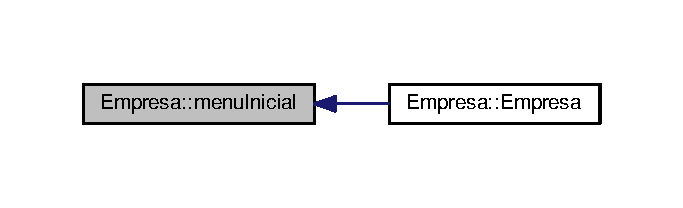
\includegraphics[width=328pt]{classEmpresa_ad77cdd5a6cbe2beb2078aa6bec2cfe28_icgraph}
\end{center}
\end{figure}


\index{Empresa@{Empresa}!menu\+Ofertas@{menu\+Ofertas}}
\index{menu\+Ofertas@{menu\+Ofertas}!Empresa@{Empresa}}
\subsubsection[{\texorpdfstring{menu\+Ofertas()}{menuOfertas()}}]{\setlength{\rightskip}{0pt plus 5cm}void Empresa\+::menu\+Ofertas (
\begin{DoxyParamCaption}
{}
\end{DoxyParamCaption}
)}\hypertarget{classEmpresa_a3cab1a61ff84c5b20ac2faa6251e25ed}{}\label{classEmpresa_a3cab1a61ff84c5b20ac2faa6251e25ed}


displays the offers Menu 


\begin{DoxyCode}
1253                           \{
1254 
1255 
1256 
1257     \textcolor{keywordtype}{int} opcaoOfertas;
1258     \textcolor{keywordflow}{while} (\textcolor{keyword}{true}) \{
1259         \hyperlink{classEmpresa_ad79f7196a8ce7256771cbd7b9542155c}{titulo}();
1260         cout << \textcolor{stringliteral}{"+----------------------------------------------------------+\(\backslash\)n"};
1261         cout << \textcolor{stringliteral}{"| Escolha o que pretende fazer com as Ofertas              |\(\backslash\)n"};
1262         cout << \textcolor{stringliteral}{"+----------------------------------------------------------+\(\backslash\)n"};
1263         cout << \textcolor{stringliteral}{"| Selecione a sua opcao (insira apenas o numero):          |\(\backslash\)n"};
1264         cout << \textcolor{stringliteral}{"+----------------------------------------------------------+\(\backslash\)n"};
1265         cout << \textcolor{stringliteral}{"| 1 - Adicionar Oferta                                     |\(\backslash\)n"};
1266         cout << \textcolor{stringliteral}{"| 2 - Modificar Oferta                                     |\(\backslash\)n"};
1267         cout << \textcolor{stringliteral}{"| 3 - Apagar Oferta                                        |\(\backslash\)n"};
1268         cout << \textcolor{stringliteral}{"| 4 - Ver Ofertas                                          |\(\backslash\)n"};
1269         cout << \textcolor{stringliteral}{"| 5 - Ver Ofertas (Ordenadas por Prioridade)               |\(\backslash\)n"};
1270         cout << \textcolor{stringliteral}{"| 6 - Ver os clientes que reservaram uma oferta específica |\(\backslash\)n"};
1271         cout << \textcolor{stringliteral}{"| 0 - Sair                                                 |\(\backslash\)n"};
1272         cout << \textcolor{stringliteral}{"+----------------------------------------------------------+\(\backslash\)n"};
1273         cin >> opcaoOfertas;
1274         \textcolor{keywordflow}{if} (cin.fail()) \{
1275             cin.clear();
1276             cin.ignore(INT\_MAX, \textcolor{charliteral}{'\(\backslash\)n'});
1277             \hyperlink{menu_8h_aceb70c1ed7e11f0863a868704f02214b}{clearScreen}();
1278             cout << \textcolor{stringliteral}{"Erro: Introduziu um input invalido. So pode usar numeros inteiros."} << endl;
1279             cout << \textcolor{stringliteral}{"Pressione Enter para voltar ao menu"} << endl;
1280             cin.get();
1281         \}
1282         \textcolor{keywordflow}{switch} (opcaoOfertas) \{
1283 
1284         \textcolor{keywordflow}{case} 1:
1285             \textcolor{keywordflow}{try} \{
1286                 \hyperlink{classEmpresa_ae244a8ae3afb85eb5e9e5febce8b8728}{adicionaOferta}();
1287             \}
1288             \textcolor{keywordflow}{catch} (\hyperlink{classObjetoRepetido}{ObjetoRepetido<Oferta>} & ex) \{
1289                 \hyperlink{menu_8h_aceb70c1ed7e11f0863a868704f02214b}{clearScreen}();
1290                 cout << \textcolor{stringliteral}{"A oferta "} << ex << \textcolor{stringliteral}{" ja existe "} << endl;
1291                 cout << \textcolor{stringliteral}{"Pressione enter para regressar ao menu"} << endl;
1292                 cin.get();
1293             \}
1294             \textcolor{keywordflow}{catch} (\hyperlink{classObjetoInexistente}{ObjetoInexistente<Fornecedor>} & ex) \{
1295                 \hyperlink{menu_8h_aceb70c1ed7e11f0863a868704f02214b}{clearScreen}();
1296                 cout << \textcolor{stringliteral}{"O fornecedor "} << ex << \textcolor{stringliteral}{" nao existe. "} << endl;
1297                 cout << \textcolor{stringliteral}{"Pressione enter para regressar ao menu"} << endl;
1298                 cin.get();
1299             \}
1300             \textcolor{keywordflow}{break};
1301         \textcolor{keywordflow}{case} 2:
1302             \textcolor{keywordflow}{try} \{
1303                 \hyperlink{classEmpresa_ac8948065c65d5c02cb30103118f502d4}{modificaOferta}();
1304             \}
1305             \textcolor{keywordflow}{catch} (\hyperlink{classObjetoInexistente}{ObjetoInexistente<Cliente>} & ex) \{
1306                 \hyperlink{menu_8h_aceb70c1ed7e11f0863a868704f02214b}{clearScreen}();
1307                 cout << \textcolor{stringliteral}{"O cliente "} << ex << \textcolor{stringliteral}{" nao existe. "} << endl;
1308                 cout << \textcolor{stringliteral}{"Pressione enter para regressar ao menu"} << endl;
1309                 cin.get();
1310             \}
1311             \textcolor{keywordflow}{catch} (\hyperlink{classObjetoInexistente}{ObjetoInexistente<Oferta>} & ex) \{
1312                 \hyperlink{menu_8h_aceb70c1ed7e11f0863a868704f02214b}{clearScreen}();
1313                 cout << \textcolor{stringliteral}{"A oferta "} << ex << \textcolor{stringliteral}{" nao existe. "} << endl;
1314                 cout << \textcolor{stringliteral}{"Pressione enter para regressar ao menu"} << endl;
1315                 cin.get();
1316 
1317             \}
1318             \textcolor{keywordflow}{break};
1319         \textcolor{keywordflow}{case} 3:
1320             \textcolor{keywordflow}{try} \{
1321                 \hyperlink{classEmpresa_a5b5c42d733ccee37f932db5db8aec243}{removeOferta}();
1322             \}
1323             \textcolor{keywordflow}{catch} (\hyperlink{classObjetoInexistente}{ObjetoInexistente<Fornecedor>} & ex) \{
1324                 \hyperlink{menu_8h_aceb70c1ed7e11f0863a868704f02214b}{clearScreen}();
1325                 cout << \textcolor{stringliteral}{"O fornecedor "} << ex << \textcolor{stringliteral}{" nao existe. "} << endl;
1326                 cout << \textcolor{stringliteral}{"Pressione enter para regressar ao menu"} << endl;
1327                 cin.get();
1328             \}
1329             \textcolor{keywordflow}{catch} (\hyperlink{classObjetoInexistente}{ObjetoInexistente<Oferta>} & ex) \{
1330                 \hyperlink{menu_8h_aceb70c1ed7e11f0863a868704f02214b}{clearScreen}();
1331                 cout << \textcolor{stringliteral}{"A oferta "} << ex << \textcolor{stringliteral}{" nao existe. "} << endl;
1332                 cout << \textcolor{stringliteral}{"Pressione enter para regressar ao menu"} << endl;
1333                 cin.get();
1334             \}
1335             \textcolor{keywordflow}{break};
1336         \textcolor{keywordflow}{case} 4:
1337             \hyperlink{classEmpresa_aa47e9a64800a41180b7f374b73a1f32b}{displayFornecedorescomOfertas}();
1338             cin.get();
1339             cin.get();
1340             \textcolor{keywordflow}{break};
1341 
1342         \textcolor{keywordflow}{case} 5:
1343             \hyperlink{classEmpresa_acd458614a3cca3f432b54212a2e72584}{displayOfertasemOrdem}();
1344             cin.get();
1345             cin.get();
1346             \textcolor{keywordflow}{break};
1347 
1348         \textcolor{keywordflow}{case} 6:
1349             \textcolor{keywordflow}{try} \{
1350                 \hyperlink{classEmpresa_a641c2eb827b39ab79919187645ff71a9}{displayTodosOsClientesdeumaOferta}();
1351             \}
1352             \textcolor{keywordflow}{catch} (\hyperlink{classObjetoInexistente}{ObjetoInexistente<Fornecedor>} & ex) \{
1353                 \hyperlink{menu_8h_aceb70c1ed7e11f0863a868704f02214b}{clearScreen}();
1354                 cout << \textcolor{stringliteral}{"O fornecedor "} << ex << \textcolor{stringliteral}{" nao existe. "} << endl;
1355                 cout << \textcolor{stringliteral}{"Pressione enter para regressar ao menu"} << endl;
1356                 cin.get();
1357             \}
1358             \textcolor{keywordflow}{catch} (\hyperlink{classObjetoInexistente}{ObjetoInexistente<Oferta>} & ex) \{
1359                 \hyperlink{menu_8h_aceb70c1ed7e11f0863a868704f02214b}{clearScreen}();
1360                 cout << \textcolor{stringliteral}{"A oferta "} << ex << \textcolor{stringliteral}{" nao existe. "} << endl;
1361                 cout << \textcolor{stringliteral}{"Pressione enter para regressar ao menu"} << endl;
1362                 cin.get();
1363             \}
1364             \textcolor{keywordflow}{catch} (\hyperlink{classObjetoInexistente}{ObjetoInexistente<Reserva>} & ex) \{
1365                 \hyperlink{menu_8h_aceb70c1ed7e11f0863a868704f02214b}{clearScreen}();
1366                 cout << \textcolor{stringliteral}{"Parece que nao foi efetuada nenhuma reserva para dessa oferta."} << endl;
1367                 cout << \textcolor{stringliteral}{"Pressione enter para regressar ao menu"} << endl;
1368                 cin.get();
1369             \}
1370                 \textcolor{keywordflow}{break};
1371             
1372         \textcolor{keywordflow}{case} 0:
1373             \textcolor{keywordflow}{return};
1374             \textcolor{keywordflow}{break};
1375 
1376         \textcolor{keywordflow}{default}:
1377             cout << \textcolor{stringliteral}{"Lamento, mas a opcao que inseriu nao e valida. Tente outra vez"} << endl;
1378             cout << \textcolor{stringliteral}{"Pressione Enter para repetir"} << endl;
1379             cin.get();
1380             \hyperlink{menu_8h_aceb70c1ed7e11f0863a868704f02214b}{clearScreen}();
1381 
1382             \}
1383 
1384         
1385     \}
1386 \}
\end{DoxyCode}
\index{Empresa@{Empresa}!menu\+Reservas@{menu\+Reservas}}
\index{menu\+Reservas@{menu\+Reservas}!Empresa@{Empresa}}
\subsubsection[{\texorpdfstring{menu\+Reservas()}{menuReservas()}}]{\setlength{\rightskip}{0pt plus 5cm}void Empresa\+::menu\+Reservas (
\begin{DoxyParamCaption}
{}
\end{DoxyParamCaption}
)}\hypertarget{classEmpresa_a0d362cb7362b859ccf99b9603de6b603}{}\label{classEmpresa_a0d362cb7362b859ccf99b9603de6b603}


displays the Reservations Menu 


\begin{DoxyCode}
798                            \{
799 
800 
801     \textcolor{keywordtype}{int} opcaoreservas;
802     \textcolor{keywordflow}{while} (\textcolor{keyword}{true}) \{
803         \hyperlink{classEmpresa_ad79f7196a8ce7256771cbd7b9542155c}{titulo}();
804         cout << \textcolor{stringliteral}{"+----------------------------------------------------------+\(\backslash\)n"};
805         cout << \textcolor{stringliteral}{"| Escolha o que pretende fazer com as reservas             |\(\backslash\)n"};
806         cout << \textcolor{stringliteral}{"+----------------------------------------------------------+\(\backslash\)n"};
807         cout << \textcolor{stringliteral}{"| Selecione a sua opcao (insira apenas o numero):          |\(\backslash\)n"};
808         cout << \textcolor{stringliteral}{"+----------------------------------------------------------+\(\backslash\)n"};
809         cout << \textcolor{stringliteral}{"| 1 - Adicionar Reserva                                    |\(\backslash\)n"};
810         cout << \textcolor{stringliteral}{"| 2 - Modificar Reserva                                    |\(\backslash\)n"};
811         cout << \textcolor{stringliteral}{"| 3 - Cancelar Reserva                                     |\(\backslash\)n"};
812         cout << \textcolor{stringliteral}{"| 4 - Apagar Reserva                                       |\(\backslash\)n"};
813         cout << \textcolor{stringliteral}{"| 5 - Ver Reservas                                         |\(\backslash\)n"};
814         cout << \textcolor{stringliteral}{"| 0 - Sair                                                 |\(\backslash\)n"};
815         cout << \textcolor{stringliteral}{"+----------------------------------------------------------+\(\backslash\)n"};
816 
817         cin >> opcaoreservas;
818 
819         \textcolor{keywordflow}{if} (cin.fail())\{
820 
821             cin.clear();
822             cin.ignore(INT\_MAX,\textcolor{charliteral}{'\(\backslash\)n'});
823             \hyperlink{menu_8h_aceb70c1ed7e11f0863a868704f02214b}{clearScreen}();
824             cout << \textcolor{stringliteral}{"Erro: Introduziu um input invalido. So pode usar numeros inteiros."} << endl;
825             cout << \textcolor{stringliteral}{"Pressione Enter para voltar ao menu"} << endl;
826             cin.get();
827             \textcolor{keywordflow}{return};
828 
829 
830 
831                 \}
832         \textcolor{keywordflow}{switch} (opcaoreservas) \{
833 
834         
835 
836         \textcolor{keywordflow}{case} 1:
837             \textcolor{keywordflow}{try}\{
838             \hyperlink{classEmpresa_a42953bdbb2fb39173ad6f38892fc122b}{adicionaReserva}();
839             \}
840             \textcolor{keywordflow}{catch}(\hyperlink{classObjetoInexistente}{ObjetoInexistente<Cliente>} & ex)\{
841                 cout << \textcolor{stringliteral}{"O cliente "} << ex << \textcolor{stringliteral}{" nao existe"} << endl;
842                 cout << \textcolor{stringliteral}{"Pressione Enter para regressar ao menu anterior"} << endl;
843                 cin.get();
844                 \textcolor{keywordflow}{return};
845             \}
846             \textcolor{keywordflow}{catch}(\hyperlink{classObjetoInexistente}{ObjetoInexistente<Fornecedor>} & ex)\{
847                 cout << \textcolor{stringliteral}{"O fornecedor "} << ex << \textcolor{stringliteral}{" nao existe"} << endl;
848                 cout << \textcolor{stringliteral}{"Pressione Enter para regressar ao menu anterior"} << endl;
849                 cin.get();
850                 \textcolor{keywordflow}{return};
851             \}
852             \textcolor{keywordflow}{catch}(\hyperlink{classObjetoInexistente}{ObjetoInexistente<Oferta>} & ex)\{
853                 cout << \textcolor{stringliteral}{"A oferta "} << ex << \textcolor{stringliteral}{" nao existe"} << endl;
854                 cout << \textcolor{stringliteral}{"Pressione Enter para regressar ao menu anterior"} << endl;
855                 cin.get();
856                 \textcolor{keywordflow}{return};
857             \}
858             \textcolor{keywordflow}{break};
859         \textcolor{keywordflow}{case} 2:
860             \textcolor{keywordflow}{try}\{
861             \hyperlink{classEmpresa_ae74f80c120a14f0591d04fe7603e6905}{modificaReserva}();
862             \}
863             \textcolor{keywordflow}{catch}(\hyperlink{classObjetoInexistente}{ObjetoInexistente<Fornecedor>} & ex)\{
864                 \hyperlink{menu_8h_aceb70c1ed7e11f0863a868704f02214b}{clearScreen}();
865                 cout << \textcolor{stringliteral}{"O fornecedor "} << ex << \textcolor{stringliteral}{" nao existe. "} << endl;
866                 cout << \textcolor{stringliteral}{"Pressione enter para regressar ao menu"} << endl;
867                 cin.get();
868             \}
869             \textcolor{keywordflow}{break};
870         \textcolor{keywordflow}{case} 3:
871             \textcolor{keywordflow}{try}\{
872             \hyperlink{classEmpresa_aa0b169a112c75b6fd1bc80128720282e}{cancelaReservas}();
873             \}
874             \textcolor{keywordflow}{catch}(\hyperlink{classObjetoInexistente}{ObjetoInexistente<Reserva>} & ex)\{
875                 \hyperlink{menu_8h_aceb70c1ed7e11f0863a868704f02214b}{clearScreen}();
876                 cout << \textcolor{stringliteral}{"A reserva indicada nao existe. "} << endl;
877                 cout << \textcolor{stringliteral}{"Pressione enter para regressar ao menu"} << endl;
878                 cin.get();
879             \}
880             \textcolor{keywordflow}{catch} (\hyperlink{classObjetoInexistente}{ObjetoInexistente<Oferta>} & ex) \{
881                 cout << \textcolor{stringliteral}{"A oferta "} << ex << \textcolor{stringliteral}{" nao existe"} << endl;
882                 cout << \textcolor{stringliteral}{"Pressione Enter para regressar ao menu anterior"} << endl;
883                 cin.get();
884                 \textcolor{keywordflow}{return};
885             \}
886             \textcolor{keywordflow}{break};
887         \textcolor{keywordflow}{case} 4:
888             \textcolor{keywordflow}{try}\{
889             \hyperlink{classEmpresa_a3e0ee0b5d92f0cd655a26095229849f1}{removeReservas}();
890             \}
891             \textcolor{keywordflow}{catch}(\hyperlink{classObjetoInexistente}{ObjetoInexistente<Reserva>} & ex)\{
892                 \hyperlink{menu_8h_aceb70c1ed7e11f0863a868704f02214b}{clearScreen}();
893                 cout << \textcolor{stringliteral}{"A reserva indicada nao existe. "} << endl;
894                 cout << \textcolor{stringliteral}{"Pressione enter para regressar ao menu"} << endl;
895                 cin.get();
896             \}
897             \textcolor{keywordflow}{break};
898         \textcolor{keywordflow}{case} 5:
899             \hyperlink{classEmpresa_a8c89e6053eaccf0e1938a4f2ab0bfdc4}{displayReservas}();
900             cin.get();
901             cin.get();
902             \textcolor{keywordflow}{break};
903         
904 
905         \textcolor{keywordflow}{case} 0:
906             \textcolor{keywordflow}{return};
907 
908         \textcolor{keywordflow}{default}:
909             cout << \textcolor{stringliteral}{"Lamento, mas a opcao que inseriu nao e valida. \(\backslash\)n"};
910             
911 
912     \}
913 \}
914     \textcolor{keywordflow}{return};
915 \}
\end{DoxyCode}
\index{Empresa@{Empresa}!menu\+Tipode\+Utilizador@{menu\+Tipode\+Utilizador}}
\index{menu\+Tipode\+Utilizador@{menu\+Tipode\+Utilizador}!Empresa@{Empresa}}
\subsubsection[{\texorpdfstring{menu\+Tipode\+Utilizador()}{menuTipodeUtilizador()}}]{\setlength{\rightskip}{0pt plus 5cm}void Empresa\+::menu\+Tipode\+Utilizador (
\begin{DoxyParamCaption}
{}
\end{DoxyParamCaption}
)}\hypertarget{classEmpresa_a544832c17fe7d592ae1d01bdc144059e}{}\label{classEmpresa_a544832c17fe7d592ae1d01bdc144059e}


Displays a menu that guides the user to all the sub-\/menus. 


\begin{DoxyCode}
1795 \{
1796     
1797     
1798     \textcolor{keywordtype}{int} tipodeutilizador;
1799     \textcolor{keywordflow}{while} (\textcolor{keyword}{true})\{
1800         \hyperlink{classEmpresa_ad79f7196a8ce7256771cbd7b9542155c}{titulo}();
1801         
1802         cout << \textcolor{stringliteral}{"+----------------------------------------------------------+\(\backslash\)n"};
1803         cout << \textcolor{stringliteral}{"| Escolha o tipo de opcao sobre o qual quer trabalhar      |\(\backslash\)n"};
1804         cout << \textcolor{stringliteral}{"+----------------------------------------------------------+\(\backslash\)n"};
1805         cout << \textcolor{stringliteral}{"| Selecione a sua opcao (insira apenas o numero):          |\(\backslash\)n"};
1806         cout << \textcolor{stringliteral}{"+----------------------------------------------------------+\(\backslash\)n"};
1807         cout << \textcolor{stringliteral}{"| 1 - Gestao de Clientes                                   |\(\backslash\)n"};
1808         cout << \textcolor{stringliteral}{"| 2 - Gestao de Fornecedores                               |\(\backslash\)n"};
1809         cout << \textcolor{stringliteral}{"| 3 - Gestao de Reservas                                   |\(\backslash\)n"};
1810         cout << \textcolor{stringliteral}{"| 4 - Gestao de Ofertas                                    |\(\backslash\)n"};
1811         cout << \textcolor{stringliteral}{"| 0 - Sair                                                 |\(\backslash\)n"};
1812         cout << \textcolor{stringliteral}{"+----------------------------------------------------------+\(\backslash\)n"};
1813 
1814         cin >> tipodeutilizador;
1815 
1816         \textcolor{keywordflow}{if} (cin.fail())\{
1817             cin.clear();
1818             cin.ignore(INT\_MAX,\textcolor{charliteral}{'\(\backslash\)n'});
1819             \hyperlink{menu_8h_aceb70c1ed7e11f0863a868704f02214b}{clearScreen}();
1820             cout << \textcolor{stringliteral}{"Erro: Introduziu um input invalido. So pode usar numeros inteiros."} << endl;
1821             cout << \textcolor{stringliteral}{"Pressione Enter para voltar ao menu"} << endl;
1822             cin.get();
1823         \}
1824 
1825         \textcolor{keywordflow}{switch} (tipodeutilizador) \{
1826 
1827         \textcolor{keywordflow}{case} 0:
1828             cout << \textcolor{stringliteral}{"\(\backslash\)n"} << \textcolor{stringliteral}{"Agradecemos a utilizacao do nosso servico, a aplicacao ira agora fechar.\(\backslash\)n"};
1829             \textcolor{keywordflow}{return};
1830             \textcolor{keywordflow}{break};
1831         \textcolor{keywordflow}{case} 1:
1832             \hyperlink{classEmpresa_a2e8e13ecd162403da0118ceccdccbbcb}{menuCliente}();
1833             \textcolor{keywordflow}{break};
1834         \textcolor{keywordflow}{case} 2:
1835             \hyperlink{classEmpresa_adb9d8d4aa55f253fc534e220ca4a87ac}{menuFornecedor}();
1836             \textcolor{keywordflow}{break};
1837 
1838         \textcolor{keywordflow}{case} 3:
1839             \hyperlink{classEmpresa_a0d362cb7362b859ccf99b9603de6b603}{menuReservas}();
1840             \textcolor{keywordflow}{break};
1841 
1842         \textcolor{keywordflow}{case} 4:
1843             \hyperlink{classEmpresa_a3cab1a61ff84c5b20ac2faa6251e25ed}{menuOfertas}();
1844             \textcolor{keywordflow}{break};
1845         \textcolor{keywordflow}{default}:
1846             \hyperlink{menu_8h_aceb70c1ed7e11f0863a868704f02214b}{clearScreen}();
1847             cout << \textcolor{stringliteral}{"Lamento, mas a opcao que inseriu nao e valida. Tente outra vez. \(\backslash\)n"};
1848             cin.get();
1849             \hyperlink{menu_8h_aceb70c1ed7e11f0863a868704f02214b}{clearScreen}();
1850         \}
1851     \}
1852     \hyperlink{classEmpresa_a5ca8821d938f11f29558ae90913de528}{addOfertasQueue}();
1853     \hyperlink{classEmpresa_a46a4898b8ae8e09bdf656b25b8ffe99d}{aplicaDesconto}();
1854 \}
\end{DoxyCode}
\index{Empresa@{Empresa}!modifica\+Cliente@{modifica\+Cliente}}
\index{modifica\+Cliente@{modifica\+Cliente}!Empresa@{Empresa}}
\subsubsection[{\texorpdfstring{modifica\+Cliente()}{modificaCliente()}}]{\setlength{\rightskip}{0pt plus 5cm}void Empresa\+::modifica\+Cliente (
\begin{DoxyParamCaption}
{}
\end{DoxyParamCaption}
)}\hypertarget{classEmpresa_a9b938f2436e95e68afce6cc04f2100bc}{}\label{classEmpresa_a9b938f2436e95e68afce6cc04f2100bc}


Modifies a cliente. 


\begin{DoxyCode}
251                               \{
252 
253     \hyperlink{classEmpresa_ad79f7196a8ce7256771cbd7b9542155c}{titulo}();
254     \textcolor{keywordtype}{string} nome\_cliente, novonome,novaMorada;
255     \textcolor{keywordtype}{int} modifica, pontos;
256 
257 
258     cout << \textcolor{stringliteral}{"+----------------------------------------------------------+\(\backslash\)n"};
259     cout << \textcolor{stringliteral}{"| Qual e o nome do cliente?                                |\(\backslash\)n"};
260     cout << \textcolor{stringliteral}{"+----------------------------------------------------------+\(\backslash\)n"};
261 
262     cin.ignore(INT\_MAX, \textcolor{charliteral}{'\(\backslash\)n'});
263     getline(cin, nome\_cliente);
264 
265 
266     \textcolor{keywordtype}{int} index = \hyperlink{extras_8h_abc85c93edf561168b5bbee8054caa388}{BinarySearch}(\_clientes, nome\_cliente);
267     \textcolor{keywordflow}{if} (index == -1) \{ \textcolor{keywordflow}{throw} \hyperlink{classObjetoInexistente}{ObjetoInexistente<Cliente>}(nome\_cliente); \}
268 
269     cout << \textcolor{stringliteral}{"+----------------------------------------------------------+\(\backslash\)n"};
270     cout << \textcolor{stringliteral}{"| Que propriedade do cliente pretende modificar?           |\(\backslash\)n"};
271     cout << \textcolor{stringliteral}{"+----------------------------------------------------------+\(\backslash\)n"};
272     cout << \textcolor{stringliteral}{"| 1 - Nome                                                 |\(\backslash\)n"};
273     cout << \textcolor{stringliteral}{"| 2 - Pontos                                               |\(\backslash\)n"};
274     cout << \textcolor{stringliteral}{"| 3 - Estatuto de Registado                                |\(\backslash\)n"};
275     cout << \textcolor{stringliteral}{"| 4 - Morada                                               |\(\backslash\)n"};
276     cout << \textcolor{stringliteral}{"| 0 - Sair                                                 |\(\backslash\)n"};
277     cout << \textcolor{stringliteral}{"+----------------------------------------------------------+\(\backslash\)n"};
278 
279     cin >> modifica;
280 
281     \textcolor{keywordflow}{switch} (modifica) \{
282     \textcolor{keywordflow}{case} 0:
283         \textcolor{keywordflow}{return};
284         \textcolor{keywordflow}{break};
285     \textcolor{keywordflow}{case} 1:
286         cout << \textcolor{stringliteral}{"+----------------------------------------------------------+\(\backslash\)n"};
287         cout << \textcolor{stringliteral}{"| Indique o novo nome:                                     |\(\backslash\)n"};
288         cout << \textcolor{stringliteral}{"+----------------------------------------------------------+\(\backslash\)n"};
289 
290         cin.ignore(INT\_MAX, \textcolor{charliteral}{'\(\backslash\)n'});
291         getline(cin, novonome);
292         \_clientes.at(index)->setNome(novonome);
293         \textcolor{keywordflow}{break};
294 
295     \textcolor{keywordflow}{case} 2:
296 
297         \textcolor{keywordflow}{if} (\_clientes.at(index)->isRegistado()) \{
298             cout << \textcolor{stringliteral}{"+----------------------------------------------------------+\(\backslash\)n"};
299             cout << \textcolor{stringliteral}{"| Indique os pontos:                                       |\(\backslash\)n"};
300             cout << \textcolor{stringliteral}{"+----------------------------------------------------------+\(\backslash\)n"};
301 
302             cin >> pontos;
303             \_clientes.at(index)->setPontos(pontos);
304         \}
305         \textcolor{keywordflow}{else} cout << \textcolor{stringliteral}{"Esse cliente nao esta registado, logo nao tem pontos. Registe-o antes de utilizar os
       pontos. \(\backslash\)n"};
306 
307         \textcolor{keywordflow}{break};
308 
309     \textcolor{keywordflow}{case} 3:
310         \textcolor{keywordflow}{if}(this->\_clientes.at(index)->isRegistado())\{
311             cout << \textcolor{stringliteral}{"O cliente ja se encontra registado"} << endl;
312             cout << \textcolor{stringliteral}{"Pressione Enter para regressar ao menu"} << endl;
313             cin.get();
314         \}
315         \textcolor{keywordflow}{else}\{
316         novonome = \_clientes.at(index)->getNome();
317         novaMorada = \_clientes.at(index)->getMorada();
318         \textcolor{keyword}{delete} \_clientes.at(index);
319         \_clientes.at(index) = \textcolor{keyword}{new} \hyperlink{classClienteRegistado}{ClienteRegistado}(novonome, novaMorada,0);
320         \}
321         \textcolor{keywordflow}{break};
322 
323     \textcolor{keywordflow}{case} 4:
324         cout << \textcolor{stringliteral}{"+----------------------------------------------------------+\(\backslash\)n"};
325         cout << \textcolor{stringliteral}{"| Indique a nova morada:                                   |\(\backslash\)n"};
326         cout << \textcolor{stringliteral}{"+----------------------------------------------------------+\(\backslash\)n"};
327         cin.ignore(INT\_MAX, \textcolor{charliteral}{'\(\backslash\)n'});
328         getline(cin, novaMorada);
329         \_clientes.at(index)->setMorada(novaMorada);
330     
331     \textcolor{keywordflow}{default}:
332         cout << \textcolor{stringliteral}{"Essa opcao nao e viavel. Pressione Enter para voltar ao menu anterior."};
333 
334     \}
335     cin.get();
336     \textcolor{keywordflow}{return};
337 
338 \}
\end{DoxyCode}


Here is the call graph for this function\+:\nopagebreak
\begin{figure}[H]
\begin{center}
\leavevmode
\includegraphics[width=350pt]{classEmpresa_a9b938f2436e95e68afce6cc04f2100bc_cgraph}
\end{center}
\end{figure}


\index{Empresa@{Empresa}!modifica\+Fornecedor@{modifica\+Fornecedor}}
\index{modifica\+Fornecedor@{modifica\+Fornecedor}!Empresa@{Empresa}}
\subsubsection[{\texorpdfstring{modifica\+Fornecedor()}{modificaFornecedor()}}]{\setlength{\rightskip}{0pt plus 5cm}void Empresa\+::modifica\+Fornecedor (
\begin{DoxyParamCaption}
{}
\end{DoxyParamCaption}
)}\hypertarget{classEmpresa_aa0470e1fd4f41615a230fc8048b8b321}{}\label{classEmpresa_aa0470e1fd4f41615a230fc8048b8b321}


Modifies a supplier. 


\begin{DoxyCode}
552                                  \{
553 
554     \hyperlink{classEmpresa_ad79f7196a8ce7256771cbd7b9542155c}{titulo}();
555     \textcolor{keywordtype}{string} nome\_fornecedor, novonome,novamorada;
556     \textcolor{keywordtype}{int} modifica;
557     \textcolor{keywordtype}{unsigned} \textcolor{keywordtype}{int} novoNIF;
558 
559 
560     cout << \textcolor{stringliteral}{"+----------------------------------------------------------+\(\backslash\)n"};
561     cout << \textcolor{stringliteral}{"| Estes sao os fornecedores:                               |\(\backslash\)n"};
562     cout << \textcolor{stringliteral}{"+----------------------------------------------------------+\(\backslash\)n"};
563 
564     \hyperlink{classEmpresa_a55c3756c01b45b41ad03f4e4f3e4dcac}{displayFornecedores}();
565 
566 
567     cout << \textcolor{stringliteral}{"+----------------------------------------------------------+\(\backslash\)n"};
568     cout << \textcolor{stringliteral}{"| Qual e o nome do fornecedor?                             |\(\backslash\)n"};
569     cout << \textcolor{stringliteral}{"+----------------------------------------------------------+\(\backslash\)n"};
570 
571     cin.ignore(INT\_MAX, \textcolor{charliteral}{'\(\backslash\)n'});
572     getline(cin, nome\_fornecedor);
573     
574 
575     \textcolor{keywordtype}{int} index = \hyperlink{extras_8h_abc85c93edf561168b5bbee8054caa388}{BinarySearch}(\_fornecedores, nome\_fornecedor);
576     \textcolor{keywordflow}{if} (index == -1) \{ \textcolor{keywordflow}{throw} \hyperlink{classObjetoInexistente}{ObjetoInexistente<Fornecedor>}(nome\_fornecedor); \}
577 
578 
579     cout << \textcolor{stringliteral}{"+----------------------------------------------------------+\(\backslash\)n"};
580     cout << \textcolor{stringliteral}{"| Que propriedade do fornecedor pretende modificar?        |\(\backslash\)n"};
581     cout << \textcolor{stringliteral}{"+----------------------------------------------------------+\(\backslash\)n"};
582     cout << \textcolor{stringliteral}{"| 1 - Nome                                                 |\(\backslash\)n"};
583     cout << \textcolor{stringliteral}{"| 2 - NIF                                                  |\(\backslash\)n"};
584     cout << \textcolor{stringliteral}{"| 3 - Morada                                               |\(\backslash\)n"};
585     cout << \textcolor{stringliteral}{"| 4 - Definicoes de Fornecedor                             |\(\backslash\)n"};
586     cout << \textcolor{stringliteral}{"| 0 - Sair                                                 |\(\backslash\)n"};
587     cout << \textcolor{stringliteral}{"+----------------------------------------------------------+\(\backslash\)n"};
588 
589     cin >> modifica;
590     
591     \textcolor{keywordflow}{switch} (modifica) \{
592     \textcolor{keywordflow}{case} 0:
593         \textcolor{keywordflow}{return};
594         \textcolor{keywordflow}{break};
595     \textcolor{keywordflow}{case} 1:
596         cout << \textcolor{stringliteral}{"+----------------------------------------------------------+\(\backslash\)n"};
597         cout << \textcolor{stringliteral}{"| Indique o novo nome:                                     |\(\backslash\)n"};
598         cout << \textcolor{stringliteral}{"+----------------------------------------------------------+\(\backslash\)n"};
599 
600         cin.ignore(INT\_MAX, \textcolor{charliteral}{'\(\backslash\)n'});
601         getline(cin, novonome);
602         \_fornecedores.at(index)->setNome(novonome);
603         \textcolor{keywordflow}{break};
604 
605     \textcolor{keywordflow}{case} 2:
606         cout << \textcolor{stringliteral}{"+----------------------------------------------------------+\(\backslash\)n"};
607         cout << \textcolor{stringliteral}{"| Indique o novo NIF:                                      |\(\backslash\)n"};
608         cout << \textcolor{stringliteral}{"+----------------------------------------------------------+\(\backslash\)n"};
609 
610         cin >> novoNIF;
611         \_fornecedores.at(index)->setNIF(novoNIF);
612         \textcolor{keywordflow}{break};
613 
614     \textcolor{keywordflow}{case} 3:
615         cout << \textcolor{stringliteral}{"+----------------------------------------------------------+\(\backslash\)n"};
616         cout << \textcolor{stringliteral}{"| Indique a nova morada:                                   |\(\backslash\)n"};
617         cout << \textcolor{stringliteral}{"+----------------------------------------------------------+\(\backslash\)n"};
618 
619         cin.ignore(INT\_MAX, \textcolor{charliteral}{'\(\backslash\)n'});
620         getline(cin, novamorada);
621         \_fornecedores.at(index)->setMorada(novamorada);
622         \textcolor{keywordflow}{break};
623     
624     \textcolor{keywordflow}{case} 4:
625         \_fornecedores.at(index)->setDefinicoesFornecedor();
626         \textcolor{keywordflow}{break};
627 
628     \textcolor{keywordflow}{default}:
629         cout << \textcolor{stringliteral}{"Essa opcao nao e viavel. Pressione Enter para voltar ao menu anterior."};
630 
631     \}
632     cin.get();
633     \textcolor{keywordflow}{return};
634 
635 \}
\end{DoxyCode}


Here is the call graph for this function\+:\nopagebreak
\begin{figure}[H]
\begin{center}
\leavevmode
\includegraphics[width=350pt]{classEmpresa_aa0470e1fd4f41615a230fc8048b8b321_cgraph}
\end{center}
\end{figure}


\index{Empresa@{Empresa}!modifica\+Oferta@{modifica\+Oferta}}
\index{modifica\+Oferta@{modifica\+Oferta}!Empresa@{Empresa}}
\subsubsection[{\texorpdfstring{modifica\+Oferta()}{modificaOferta()}}]{\setlength{\rightskip}{0pt plus 5cm}void Empresa\+::modifica\+Oferta (
\begin{DoxyParamCaption}
{}
\end{DoxyParamCaption}
)}\hypertarget{classEmpresa_ac8948065c65d5c02cb30103118f502d4}{}\label{classEmpresa_ac8948065c65d5c02cb30103118f502d4}


displays the interface to modify offers 


\begin{DoxyCode}
1575 \{
1576 
1577     \hyperlink{classEmpresa_ad79f7196a8ce7256771cbd7b9542155c}{titulo}();
1578     \textcolor{keywordtype}{int} modifica, indexOferta = -1;
1579     \textcolor{keywordtype}{string} nomeCliente, nomeOferta, novonome, novobarco, novahora, novodestino, temp;
1580     \textcolor{keywordtype}{unsigned} \textcolor{keywordtype}{int} novopreco, novalotacao, novadistancia;
1581     std::vector<std::string> novosdestinos;
1582     \hyperlink{classTime}{Time} *tempo;
1583 
1584     \hyperlink{classEmpresa_aa47e9a64800a41180b7f374b73a1f32b}{displayFornecedorescomOfertas}();
1585     
1586     cout << \textcolor{stringliteral}{"+----------------------------------------------------------+\(\backslash\)n"};
1587     cout << \textcolor{stringliteral}{"| Indique o nome do fornecedor cuja oferta quer alterar:   |\(\backslash\)n"};
1588     cout << \textcolor{stringliteral}{"+----------------------------------------------------------+\(\backslash\)n"};
1589 
1590     cin.ignore(INT\_MAX, \textcolor{charliteral}{'\(\backslash\)n'});
1591     getline(cin, nomeCliente);
1592 
1593     \textcolor{keywordtype}{int} index = \hyperlink{extras_8h_abc85c93edf561168b5bbee8054caa388}{BinarySearch}(\_fornecedores, nomeCliente);
1594     \textcolor{keywordflow}{if} (index == -1) \{ \textcolor{keywordflow}{throw} \hyperlink{classObjetoInexistente}{ObjetoInexistente<Fornecedor>}(nomeCliente); \}
1595     
1596 
1597     cout << \textcolor{stringliteral}{"+----------------------------------------------------------+\(\backslash\)n"};
1598     cout << \textcolor{stringliteral}{"| Indique o nome da oferta em questao:                     |\(\backslash\)n"};
1599     cout << \textcolor{stringliteral}{"+----------------------------------------------------------+\(\backslash\)n"};
1600 
1601     getline(cin, nomeOferta);
1602 
1603     indexOferta = -1;
1604     \textcolor{keywordflow}{for} (\textcolor{keywordtype}{unsigned} \textcolor{keywordtype}{int} i = 0; i <\_fornecedores.at(index)->getOfertas().size(); i++)
1605     \{
1606         
1607         \textcolor{keywordflow}{if} (\_fornecedores.at(index)->getOfertas().at(i).getNome() == nomeOferta)
1608         \{
1609             indexOferta = i;
1610         \}
1611     \}
1612     \textcolor{keywordflow}{if}(indexOferta == -1)\{ \textcolor{keywordflow}{throw} \hyperlink{classObjetoInexistente}{ObjetoInexistente<Oferta>}(nomeOferta); \}
1613 
1614     cout << \textcolor{stringliteral}{"+----------------------------------------------------------+\(\backslash\)n"};
1615     cout << \textcolor{stringliteral}{"| Que propriedade da oferta retende modificar?             |\(\backslash\)n"};
1616     cout << \textcolor{stringliteral}{"+----------------------------------------------------------+\(\backslash\)n"};
1617     cout << \textcolor{stringliteral}{"| 1 - Nome                                                 |\(\backslash\)n"};
1618     cout << \textcolor{stringliteral}{"| 2 - Tipo de Barco                                        |\(\backslash\)n"};
1619     cout << \textcolor{stringliteral}{"| 3 - Destinos                                             |\(\backslash\)n"};
1620     cout << \textcolor{stringliteral}{"| 4 - Distancia                                            |\(\backslash\)n"};
1621     cout << \textcolor{stringliteral}{"| 5 - Lotacao                                              |\(\backslash\)n"};
1622     cout << \textcolor{stringliteral}{"| 6 - Data e Hora                                          |\(\backslash\)n"};
1623     cout << \textcolor{stringliteral}{"| 7 - Preco                                                |\(\backslash\)n"};
1624     cout << \textcolor{stringliteral}{"| 0 - Sair                                                 |\(\backslash\)n"};
1625     cout << \textcolor{stringliteral}{"+----------------------------------------------------------+\(\backslash\)n"};
1626 
1627     cin >> modifica;
1628 
1629     \textcolor{keywordflow}{switch} (modifica) \{
1630     \textcolor{keywordflow}{case} 0:
1631         \textcolor{keywordflow}{return};
1632         \textcolor{keywordflow}{break};
1633     \textcolor{keywordflow}{case} 1:
1634         cout << \textcolor{stringliteral}{"+----------------------------------------------------------+\(\backslash\)n"};
1635         cout << \textcolor{stringliteral}{"| Indique o novo nome:                                     |\(\backslash\)n"};
1636         cout << \textcolor{stringliteral}{"+----------------------------------------------------------+\(\backslash\)n"};
1637 
1638         cin.ignore(INT\_MAX, \textcolor{charliteral}{'\(\backslash\)n'});
1639         getline(cin, novonome);
1640         \_fornecedores.at(index)->getOfertas().at(indexOferta).setNome(novonome);
1641         \textcolor{keywordflow}{break};
1642 
1643     \textcolor{keywordflow}{case} 2:
1644 
1645         cout << \textcolor{stringliteral}{"+----------------------------------------------------------+\(\backslash\)n"};
1646         cout << \textcolor{stringliteral}{"| Escolha o tipo de barco:                                 |\(\backslash\)n"};
1647         cout << \textcolor{stringliteral}{"+----------------------------------------------------------+\(\backslash\)n"};
1648         cout << \textcolor{stringliteral}{"| 1 - Iate                                                 |\(\backslash\)n"};
1649         cout << \textcolor{stringliteral}{"| 2 - Barco Rabelo                                         |\(\backslash\)n"};
1650         cout << \textcolor{stringliteral}{"| 3 - Veleiro                                              |\(\backslash\)n"};
1651         cout << \textcolor{stringliteral}{"+----------------------------------------------------------+\(\backslash\)n"};
1652 
1653         \textcolor{keywordtype}{int} numeroBarco;
1654         cin >> numeroBarco;
1655         \textcolor{keywordflow}{if} (numeroBarco == 1) \{
1656             novobarco = \textcolor{stringliteral}{"iate"};
1657             \_fornecedores.at(index)->getOfertas().at(indexOferta).setBarco(novobarco);
1658         \}
1659         \textcolor{keywordflow}{else} \textcolor{keywordflow}{if} (numeroBarco == 2) \{
1660             novobarco = \textcolor{stringliteral}{"barco rabelo"};
1661             \_fornecedores.at(index)->getOfertas().at(indexOferta).setBarco(novobarco);
1662         \}
1663         \textcolor{keywordflow}{else} \textcolor{keywordflow}{if} (numeroBarco == 3) \{
1664             novobarco = \textcolor{stringliteral}{"veleiro"};
1665             \_fornecedores.at(index)->getOfertas().at(indexOferta).setBarco(novobarco);
1666         \}
1667         \textcolor{keywordflow}{else}
1668             cout << \textcolor{stringliteral}{"Esse número nao é reconhecido como barco."};
1669         \textcolor{keywordflow}{break};
1670         \textcolor{keywordflow}{return};
1671 
1672 
1673 
1674     \textcolor{keywordflow}{case} 3:
1675         cout << \textcolor{stringliteral}{"+----------------------------------------------------------+\(\backslash\)n"};
1676         cout << \textcolor{stringliteral}{"| Indique os novos destinos (os anteriores serao apagados):|\(\backslash\)n"};
1677         cout << \textcolor{stringliteral}{"| Para terminar, escreva FIM                               |\(\backslash\)n"};
1678         cout << \textcolor{stringliteral}{"+----------------------------------------------------------+\(\backslash\)n"};
1679         \_fornecedores.at(index)->getOfertas().at(indexOferta).apagaDestinos();
1680         cin.ignore(INT\_MAX, \textcolor{charliteral}{'\(\backslash\)n'});
1681 
1682         \textcolor{keywordflow}{while} (temp != \textcolor{stringliteral}{"FIM"})
1683         \{
1684             getline(cin, temp);
1685             \textcolor{keywordflow}{if} (temp != \textcolor{stringliteral}{"FIM"}) \{
1686                 novosdestinos.push\_back(temp);
1687             \}
1688             cout << \textcolor{stringliteral}{"\(\backslash\)n"};
1689         \}
1690         \_fornecedores.at(index)->getOfertas().at(indexOferta).setDestinos(novosdestinos);
1691         \textcolor{keywordflow}{break};
1692 
1693     \textcolor{keywordflow}{case} 4:
1694         cout << \textcolor{stringliteral}{"+----------------------------------------------------------+\(\backslash\)n"};
1695         cout << \textcolor{stringliteral}{"| Indique a nova distancia:                                |\(\backslash\)n"};
1696         cout << \textcolor{stringliteral}{"+----------------------------------------------------------+\(\backslash\)n"};
1697         cin >> novadistancia;
1698         \_fornecedores.at(index)->getOfertas().at(indexOferta).setDistancia(novadistancia);
1699         \textcolor{keywordflow}{break};
1700 
1701     \textcolor{keywordflow}{case} 5:
1702         cout << \textcolor{stringliteral}{"+----------------------------------------------------------+\(\backslash\)n"};
1703         cout << \textcolor{stringliteral}{"| Indique a nova lotacao total:                            |\(\backslash\)n"};
1704         cout << \textcolor{stringliteral}{"+----------------------------------------------------------+\(\backslash\)n"};
1705         cin >> novalotacao;
1706         \_fornecedores.at(index)->getOfertas().at(indexOferta).setLotacao(novalotacao);
1707         \textcolor{keywordflow}{break};
1708 
1709     \textcolor{keywordflow}{case} 6:
1710 
1711         cout << \textcolor{stringliteral}{"+----------------------------------------------------------+\(\backslash\)n"};
1712         cout << \textcolor{stringliteral}{"| Indique a data da viagem (YY/MM/DD H:M):                 |\(\backslash\)n"};
1713         cout << \textcolor{stringliteral}{"+----------------------------------------------------------+\(\backslash\)n"};
1714 
1715         cin.ignore(INT\_MAX, \textcolor{charliteral}{'\(\backslash\)n'});
1716         getline(cin, novahora);
1717         tempo = \textcolor{keyword}{new} \hyperlink{classTime}{Time}(novahora);
1718         \_fornecedores.at(index)->getOfertas().at(indexOferta).setTime(*tempo);
1719         \textcolor{keywordflow}{break};
1720 
1721 
1722 
1723     \textcolor{keywordflow}{case} 7:
1724         cout << \textcolor{stringliteral}{"+----------------------------------------------------------+\(\backslash\)n"};
1725         cout << \textcolor{stringliteral}{"| Indique o novo preco total:                              |\(\backslash\)n"};
1726         cout << \textcolor{stringliteral}{"+----------------------------------------------------------+\(\backslash\)n"};
1727         cin >> novopreco;
1728         \_fornecedores.at(index)->getOfertas().at(indexOferta).setPreco(novopreco);
1729         \textcolor{keywordflow}{break};
1730 
1731 
1732     \textcolor{keywordflow}{default}:
1733         cout << \textcolor{stringliteral}{"Essa opcao nao é viável. Pressione Enter para voltar ao menu anterior."};
1734 
1735     \}
1736     cin.get();
1737     \textcolor{keywordflow}{return};
1738 
1739     \hyperlink{classEmpresa_a5ca8821d938f11f29558ae90913de528}{addOfertasQueue}();
1740     \hyperlink{classEmpresa_a46a4898b8ae8e09bdf656b25b8ffe99d}{aplicaDesconto}();
1741 \}
\end{DoxyCode}


Here is the call graph for this function\+:\nopagebreak
\begin{figure}[H]
\begin{center}
\leavevmode
\includegraphics[width=350pt]{classEmpresa_ac8948065c65d5c02cb30103118f502d4_cgraph}
\end{center}
\end{figure}


\index{Empresa@{Empresa}!modifica\+Reserva@{modifica\+Reserva}}
\index{modifica\+Reserva@{modifica\+Reserva}!Empresa@{Empresa}}
\subsubsection[{\texorpdfstring{modifica\+Reserva()}{modificaReserva()}}]{\setlength{\rightskip}{0pt plus 5cm}void Empresa\+::modifica\+Reserva (
\begin{DoxyParamCaption}
{}
\end{DoxyParamCaption}
)}\hypertarget{classEmpresa_ae74f80c120a14f0591d04fe7603e6905}{}\label{classEmpresa_ae74f80c120a14f0591d04fe7603e6905}


displays the interface to modify reservations 


\begin{DoxyCode}
1064 \{
1065     \hyperlink{classEmpresa_ad79f7196a8ce7256771cbd7b9542155c}{titulo}();
1066     \textcolor{keywordtype}{string} nome\_fornecedor, novonome, novamorada;
1067     \textcolor{keywordtype}{int} modifica;
1068     \textcolor{keywordtype}{unsigned} \textcolor{keywordtype}{int} novoNIF;
1069 
1070 
1071     cout << \textcolor{stringliteral}{"+----------------------------------------------------------+\(\backslash\)n"};
1072     cout << \textcolor{stringliteral}{"| Qual e o nome do fornecedor?                             |\(\backslash\)n"};
1073     cout << \textcolor{stringliteral}{"+----------------------------------------------------------+\(\backslash\)n"};
1074 
1075     cin.ignore(INT\_MAX, \textcolor{charliteral}{'\(\backslash\)n'});
1076     getline(cin, nome\_fornecedor);
1077 
1078 
1079     \textcolor{keywordtype}{int} index = \hyperlink{extras_8h_abc85c93edf561168b5bbee8054caa388}{BinarySearch}(\_fornecedores, nome\_fornecedor);
1080     \textcolor{keywordflow}{if} (index == -1) \{ \textcolor{keywordflow}{throw} \hyperlink{classObjetoInexistente}{ObjetoInexistente<Fornecedor>}(nome\_fornecedor); \}
1081 
1082 
1083     cout << \textcolor{stringliteral}{"+----------------------------------------------------------+\(\backslash\)n"};
1084     cout << \textcolor{stringliteral}{"| Que propriedade do fornecedor pretende modificar?        |\(\backslash\)n"};
1085     cout << \textcolor{stringliteral}{"+----------------------------------------------------------+\(\backslash\)n"};
1086     cout << \textcolor{stringliteral}{"| 1 - Nome                                                 |\(\backslash\)n"};
1087     cout << \textcolor{stringliteral}{"| 2 - NIF                                                  |\(\backslash\)n"};
1088     cout << \textcolor{stringliteral}{"| 3 - Morada                                               |\(\backslash\)n"};
1089     cout << \textcolor{stringliteral}{"| 4 - Definicoes de Fornecedor                             |\(\backslash\)n"};
1090     cout << \textcolor{stringliteral}{"| 0 - Sair                                                 |\(\backslash\)n"};
1091     cout << \textcolor{stringliteral}{"+----------------------------------------------------------+\(\backslash\)n"};
1092 
1093     cin >> modifica;
1094 
1095     \textcolor{keywordflow}{switch} (modifica) \{
1096     \textcolor{keywordflow}{case} 0:
1097         \textcolor{keywordflow}{return};
1098         \textcolor{keywordflow}{break};
1099     \textcolor{keywordflow}{case} 1:
1100         cout << \textcolor{stringliteral}{"+----------------------------------------------------------+\(\backslash\)n"};
1101         cout << \textcolor{stringliteral}{"| Indique o novo nome:                                     |\(\backslash\)n"};
1102         cout << \textcolor{stringliteral}{"+----------------------------------------------------------+\(\backslash\)n"};
1103 
1104         cin.ignore(INT\_MAX, \textcolor{charliteral}{'\(\backslash\)n'});
1105         getline(cin, novonome);
1106         \_fornecedores.at(index)->setNome(novonome);
1107         \textcolor{keywordflow}{break};
1108 
1109     \textcolor{keywordflow}{case} 2:
1110         cout << \textcolor{stringliteral}{"+----------------------------------------------------------+\(\backslash\)n"};
1111         cout << \textcolor{stringliteral}{"| Indique o novo NIF:                                      |\(\backslash\)n"};
1112         cout << \textcolor{stringliteral}{"+----------------------------------------------------------+\(\backslash\)n"};
1113 
1114         cin >> novoNIF;
1115         \_fornecedores.at(index)->setNIF(novoNIF);
1116         \textcolor{keywordflow}{break};
1117 
1118     \textcolor{keywordflow}{case} 3:
1119         cout << \textcolor{stringliteral}{"+----------------------------------------------------------+\(\backslash\)n"};
1120         cout << \textcolor{stringliteral}{"| Indique a nova morada:                                   |\(\backslash\)n"};
1121         cout << \textcolor{stringliteral}{"+----------------------------------------------------------+\(\backslash\)n"};
1122 
1123         cin.ignore(INT\_MAX, \textcolor{charliteral}{'\(\backslash\)n'});
1124         getline(cin, novamorada);
1125         \_fornecedores.at(index)->setMorada(novamorada);
1126         \textcolor{keywordflow}{break};
1127 
1128     \textcolor{keywordflow}{case} 4:
1129         \_fornecedores.at(index)->setDefinicoesFornecedor();
1130         \textcolor{keywordflow}{break};
1131 
1132     \textcolor{keywordflow}{default}:
1133         cout << \textcolor{stringliteral}{"Essa opcao nao e viavel. Pressione Enter para voltar ao menu anterior."};
1134 
1135     \}
1136     cin.get();
1137     \textcolor{keywordflow}{return};
1138 
1139 \}
\end{DoxyCode}


Here is the call graph for this function\+:\nopagebreak
\begin{figure}[H]
\begin{center}
\leavevmode
\includegraphics[width=350pt]{classEmpresa_ae74f80c120a14f0591d04fe7603e6905_cgraph}
\end{center}
\end{figure}


\index{Empresa@{Empresa}!reativa\+Cliente@{reativa\+Cliente}}
\index{reativa\+Cliente@{reativa\+Cliente}!Empresa@{Empresa}}
\subsubsection[{\texorpdfstring{reativa\+Cliente(\+Cliente $\ast$c)}{reativaCliente(Cliente *c)}}]{\setlength{\rightskip}{0pt plus 5cm}{\bf Empresa} \& Empresa\+::reativa\+Cliente (
\begin{DoxyParamCaption}
\item[{{\bf Cliente} $\ast$}]{c}
\end{DoxyParamCaption}
)}\hypertarget{classEmpresa_a64b9a495ca3a80380646814557be4924}{}\label{classEmpresa_a64b9a495ca3a80380646814557be4924}


Makes a client active again. 


\begin{DoxyParams}{Parameters}
{\em c} & The client\\
\hline
\end{DoxyParams}
\begin{DoxyReturn}{Returns}
The modified company 
\end{DoxyReturn}

\begin{DoxyCode}
628                                             \{
629     \hyperlink{classClienteInativo}{ClienteInativo} ci(c);
630     this->\_clientesInativos.erase(ci);
631     \textcolor{keywordflow}{return} *\textcolor{keyword}{this};
632 \}
\end{DoxyCode}
\index{Empresa@{Empresa}!remove\+Cliente@{remove\+Cliente}}
\index{remove\+Cliente@{remove\+Cliente}!Empresa@{Empresa}}
\subsubsection[{\texorpdfstring{remove\+Cliente()}{removeCliente()}}]{\setlength{\rightskip}{0pt plus 5cm}void Empresa\+::remove\+Cliente (
\begin{DoxyParamCaption}
{}
\end{DoxyParamCaption}
)}\hypertarget{classEmpresa_ab9af9446d6d2c206b4b3e18e1bcb6475}{}\label{classEmpresa_ab9af9446d6d2c206b4b3e18e1bcb6475}


Removes a cliente. 


\begin{DoxyCode}
340                             \{
341     \hyperlink{classEmpresa_ad79f7196a8ce7256771cbd7b9542155c}{titulo}();
342 
343     \hyperlink{classEmpresa_a28e04d59daa7206bec6055249ce17410}{displayClientes}();
344     \textcolor{keywordtype}{string} clienteremover;
345     cout << \textcolor{stringliteral}{"+----------------------------------------------------------+\(\backslash\)n"};
346     cout << \textcolor{stringliteral}{"| Qual e o cliente a remover?                              |\(\backslash\)n"};
347     cout << \textcolor{stringliteral}{"+----------------------------------------------------------+\(\backslash\)n"};
348 
349     cin.ignore(INT\_MAX, \textcolor{charliteral}{'\(\backslash\)n'});
350     getline(cin, clienteremover);
351     
352 
353         \textcolor{keywordtype}{int} index = \hyperlink{extras_8h_abc85c93edf561168b5bbee8054caa388}{BinarySearch}(\_clientes, clienteremover);
354         \textcolor{keywordflow}{if} (index == -1) \{ \textcolor{keywordflow}{throw} \hyperlink{classObjetoInexistente}{ObjetoInexistente<Cliente>}(clienteremover); \}
355 
356 
357     \hyperlink{classEmpresa_a52b9f4d94c2a05704d74854ed4dd1590}{deleteClientes}(clienteremover);
358     cout << endl << \textcolor{stringliteral}{"O cliente foi removido com sucesso"} << endl;
359     cout << \textcolor{stringliteral}{"Pressione Enter para regressar"} << endl;
360     cin.get();
361     \textcolor{keywordflow}{return};
362     
363 
364 \}
\end{DoxyCode}


Here is the call graph for this function\+:\nopagebreak
\begin{figure}[H]
\begin{center}
\leavevmode
\includegraphics[width=350pt]{classEmpresa_ab9af9446d6d2c206b4b3e18e1bcb6475_cgraph}
\end{center}
\end{figure}


\index{Empresa@{Empresa}!remove\+Fornecedor@{remove\+Fornecedor}}
\index{remove\+Fornecedor@{remove\+Fornecedor}!Empresa@{Empresa}}
\subsubsection[{\texorpdfstring{remove\+Fornecedor()}{removeFornecedor()}}]{\setlength{\rightskip}{0pt plus 5cm}void Empresa\+::remove\+Fornecedor (
\begin{DoxyParamCaption}
{}
\end{DoxyParamCaption}
)}\hypertarget{classEmpresa_a9aa7b7e699971eb2e28f0db99c6500c4}{}\label{classEmpresa_a9aa7b7e699971eb2e28f0db99c6500c4}


Removes a supplier. 


\begin{DoxyCode}
636                                \{
637     \hyperlink{classEmpresa_ad79f7196a8ce7256771cbd7b9542155c}{titulo}();
638 
639     \textcolor{keywordtype}{string} fornecedorremover;
640 
641     cout << \textcolor{stringliteral}{"+----------------------------------------------------------+\(\backslash\)n"};
642     cout << \textcolor{stringliteral}{"| Estes sao os fornecedores:                               |\(\backslash\)n"};
643     cout << \textcolor{stringliteral}{"+----------------------------------------------------------+\(\backslash\)n"};
644 
645     \hyperlink{classEmpresa_a55c3756c01b45b41ad03f4e4f3e4dcac}{displayFornecedores}();
646     
647     
648     cout << \textcolor{stringliteral}{"+----------------------------------------------------------+\(\backslash\)n"};
649     cout << \textcolor{stringliteral}{"| Qual e o fornecedor a remover?                           |\(\backslash\)n"};
650     cout << \textcolor{stringliteral}{"+----------------------------------------------------------+\(\backslash\)n"};
651 
652     cin.ignore(INT\_MAX, \textcolor{charliteral}{'\(\backslash\)n'});
653     getline(cin, fornecedorremover);
654     \textcolor{keywordflow}{for} (\textcolor{keywordtype}{unsigned} \textcolor{keywordtype}{int} i = 0; i < \_fornecedores.size(); i++)
655     \{
656         \textcolor{keywordflow}{if} (\_fornecedores.at(i)->getNome() == fornecedorremover)
657         \{
658             \hyperlink{classEmpresa_ab8b7dda77caceec58e464c16b7e45f7c}{deleteFornecedores}(fornecedorremover);
659             cout << endl << \textcolor{stringliteral}{"O fornecedor foi removido com sucesso"} << endl;
660             cout << \textcolor{stringliteral}{"Pressione Enter para regressar"} << endl;
661             cin.get();
662             \textcolor{keywordflow}{return};
663         \}
664     \}
665 
666     cout << endl << \textcolor{stringliteral}{"O fornecedor com esse nome nao foi encontrado"} << endl;
667     cout << \textcolor{stringliteral}{"Pressione Enter para regressar"} << endl;
668 
669     cin.get();
670     \textcolor{keywordflow}{return};
671 \}
\end{DoxyCode}
\index{Empresa@{Empresa}!remove\+Oferta@{remove\+Oferta}}
\index{remove\+Oferta@{remove\+Oferta}!Empresa@{Empresa}}
\subsubsection[{\texorpdfstring{remove\+Oferta()}{removeOferta()}}]{\setlength{\rightskip}{0pt plus 5cm}void Empresa\+::remove\+Oferta (
\begin{DoxyParamCaption}
{}
\end{DoxyParamCaption}
)}\hypertarget{classEmpresa_a5b5c42d733ccee37f932db5db8aec243}{}\label{classEmpresa_a5b5c42d733ccee37f932db5db8aec243}


displays the interface to remove offers 


\begin{DoxyCode}
1743                            \{
1744 
1745 
1746     \hyperlink{classEmpresa_ad79f7196a8ce7256771cbd7b9542155c}{titulo}();
1747 
1748     \textcolor{keywordtype}{string} ofertaremover, nomeFornecedor;
1749     \textcolor{keywordtype}{bool} nfound = \textcolor{keyword}{true};
1750 
1751 
1752     cout << \textcolor{stringliteral}{"+----------------------------------------------------------+\(\backslash\)n"};
1753     cout << \textcolor{stringliteral}{"| Qual e o fornecedor com a oferta a remover?              |\(\backslash\)n"};
1754     cout << \textcolor{stringliteral}{"+----------------------------------------------------------+\(\backslash\)n"};
1755 
1756     \hyperlink{classEmpresa_aa47e9a64800a41180b7f374b73a1f32b}{displayFornecedorescomOfertas}();
1757 
1758     cin.ignore(INT\_MAX, \textcolor{charliteral}{'\(\backslash\)n'});
1759     getline(cin, nomeFornecedor);
1760 
1761 
1762     \textcolor{keywordtype}{int} index = \hyperlink{extras_8h_abc85c93edf561168b5bbee8054caa388}{BinarySearch}(\_fornecedores, nomeFornecedor);
1763     \textcolor{keywordflow}{if} (index == -1) \{ \textcolor{keywordflow}{throw} \hyperlink{classObjetoInexistente}{ObjetoInexistente<Fornecedor>}(nomeFornecedor); \}
1764 
1765 
1766     cout << \textcolor{stringliteral}{"+----------------------------------------------------------+\(\backslash\)n"};
1767     cout << \textcolor{stringliteral}{"| Estas sao as ofertas desse fornecedor:                   |\(\backslash\)n"};
1768     cout << \textcolor{stringliteral}{"+----------------------------------------------------------+\(\backslash\)n"};
1769     \_fornecedores.at(index)->displayOfertas();
1770 
1771     cout << \textcolor{stringliteral}{"+----------------------------------------------------------+\(\backslash\)n"};
1772     cout << \textcolor{stringliteral}{"| Qual e a oferta a remover?                               |\(\backslash\)n"};
1773     cout << \textcolor{stringliteral}{"+----------------------------------------------------------+\(\backslash\)n"};
1774 
1775 
1776     
1777 
1778     getline(cin,ofertaremover);
1779     \textcolor{keywordflow}{for} (\textcolor{keywordtype}{unsigned} \textcolor{keywordtype}{int} i = 0; i < \_fornecedores.at(index)->getOfertas().size(); i++)
1780     \{
1781         \textcolor{keywordflow}{if} (ofertaremover == \_fornecedores.at(index)->getOfertas().at(i).getNome())\{
1782             \_fornecedores.at(index)->getOfertas().erase(\_fornecedores.at(index)->getOfertas().begin() + i);
1783             nfound = \textcolor{keyword}{false}; 
1784         \}
1785     \}
1786     \textcolor{keywordflow}{if}(nfound)\{
1787         \textcolor{keywordflow}{throw} \hyperlink{classObjetoInexistente}{ObjetoInexistente<Oferta>}(ofertaremover);
1788     \}
1789     cout << \textcolor{stringliteral}{"Oferta removida com sucesso"} << endl;
1790     cout << \textcolor{stringliteral}{"Pressione Enter para regressar"} << endl;
1791 
1792 \}
\end{DoxyCode}


Here is the call graph for this function\+:\nopagebreak
\begin{figure}[H]
\begin{center}
\leavevmode
\includegraphics[width=350pt]{classEmpresa_a5b5c42d733ccee37f932db5db8aec243_cgraph}
\end{center}
\end{figure}


\index{Empresa@{Empresa}!remove\+Reservas@{remove\+Reservas}}
\index{remove\+Reservas@{remove\+Reservas}!Empresa@{Empresa}}
\subsubsection[{\texorpdfstring{remove\+Reservas()}{removeReservas()}}]{\setlength{\rightskip}{0pt plus 5cm}void Empresa\+::remove\+Reservas (
\begin{DoxyParamCaption}
{}
\end{DoxyParamCaption}
)}\hypertarget{classEmpresa_a3e0ee0b5d92f0cd655a26095229849f1}{}\label{classEmpresa_a3e0ee0b5d92f0cd655a26095229849f1}


displays the interface to remove reservations 


\begin{DoxyCode}
1141                              \{
1142     \hyperlink{classEmpresa_ad79f7196a8ce7256771cbd7b9542155c}{titulo}();
1143     \textcolor{keywordtype}{bool} nfound = \textcolor{keyword}{true};
1144 
1145     cout << \textcolor{stringliteral}{"+----------------------------------------------------------+\(\backslash\)n"};
1146     cout << \textcolor{stringliteral}{"| Estas sao as reservas disponiveis para remover:          |\(\backslash\)n"};
1147     cout << \textcolor{stringliteral}{"+----------------------------------------------------------+\(\backslash\)n"};
1148 
1149     \hyperlink{classEmpresa_a8c89e6053eaccf0e1938a4f2ab0bfdc4}{displayReservas}();
1150 
1151     \textcolor{keywordtype}{string} reservaremoveOferta, reservaremoveCliente;
1152     cout << \textcolor{stringliteral}{"+----------------------------------------------------------+\(\backslash\)n"};
1153     cout << \textcolor{stringliteral}{"| Indique o nome do cliente cuja oferta quer remover:      |\(\backslash\)n"};
1154     cout << \textcolor{stringliteral}{"+----------------------------------------------------------+\(\backslash\)n"};
1155 
1156     cin.ignore(INT\_MAX, \textcolor{charliteral}{'\(\backslash\)n'});
1157     getline(cin, reservaremoveCliente);
1158 
1159 
1160     cout << \textcolor{stringliteral}{"+----------------------------------------------------------+\(\backslash\)n"};
1161     cout << \textcolor{stringliteral}{"| Indique o nome da oferta reservada pelo cliente:         |\(\backslash\)n"};
1162     cout << \textcolor{stringliteral}{"+----------------------------------------------------------+\(\backslash\)n"};
1163 
1164 
1165     getline(cin, reservaremoveOferta);
1166 
1167     \textcolor{keywordflow}{for} (\textcolor{keywordtype}{unsigned} \textcolor{keywordtype}{int} i = 0; i < \_reservas.size(); i++)
1168     \{
1169         \textcolor{keywordflow}{if} (\_reservas.at(i)->getOferta()->getNome() == reservaremoveOferta && \_reservas.at(i)->getCliente()
      ->getNome() == reservaremoveCliente)
1170         \{
1171             \hyperlink{classEmpresa_a079c008b006f56faac3c1016fe770e8c}{deleteReservas}(reservaremoveOferta);
1172             nfound = \textcolor{keyword}{false};
1173         \}
1174     \}
1175     \textcolor{keywordflow}{if}(nfound)\{
1176         \textcolor{keywordflow}{throw} \hyperlink{classObjetoInexistente}{ObjetoInexistente<Reserva>}(\textcolor{stringliteral}{""});
1177     \}
1178 
1179     cout << \textcolor{stringliteral}{"+----------------------------------------------------------+\(\backslash\)n"};
1180     cout << \textcolor{stringliteral}{"| Reserva apagada com sucesso!                             |\(\backslash\)n"};
1181     cout << \textcolor{stringliteral}{"| Pressione a tecla Enter para sair                        |\(\backslash\)n"};
1182     cout << \textcolor{stringliteral}{"+----------------------------------------------------------+\(\backslash\)n"};
1183 
1184     cin.get();
1185     \textcolor{keywordflow}{return};
1186 \}
\end{DoxyCode}
\index{Empresa@{Empresa}!save@{save}}
\index{save@{save}!Empresa@{Empresa}}
\subsubsection[{\texorpdfstring{save()}{save()}}]{\setlength{\rightskip}{0pt plus 5cm}void Empresa\+::save (
\begin{DoxyParamCaption}
{}
\end{DoxyParamCaption}
)}\hypertarget{classEmpresa_afbde694da902870437443de43dae8071}{}\label{classEmpresa_afbde694da902870437443de43dae8071}


stores in a text file all the information generated by the program execution 


\begin{DoxyCode}
334                   \{
335     ofstream clientes\_file(\textcolor{stringliteral}{"clientes.txt"});
336     ofstream registados\_file(\textcolor{stringliteral}{"clientes\_registados.txt"});
337     ofstream fornecedores\_file(\textcolor{stringliteral}{"fornecedores.txt"});
338     ofstream reservas\_file(\textcolor{stringliteral}{"reservas.txt"});
339     \textcolor{keywordflow}{if}(!clientes\_file.is\_open())\{
340         cout << \textcolor{stringliteral}{"O programa nao consegue abrir o ficheiro de clientes"} << endl;
341         \textcolor{keywordflow}{return};
342     \}
343     \textcolor{keywordflow}{if}(!registados\_file.is\_open())\{
344         cout << \textcolor{stringliteral}{"O programa nao consegue abrir o ficheiro de clientes registados"} << endl;
345         \textcolor{keywordflow}{return};
346     \}
347     \textcolor{keywordflow}{if}(!fornecedores\_file.is\_open())\{
348         cout << \textcolor{stringliteral}{"O programa nao consegue abrir o ficheiro de fornecedores"} << endl;
349         \textcolor{keywordflow}{return};
350     \}
351     \textcolor{keywordflow}{if}(!reservas\_file.is\_open())\{
352         cout << \textcolor{stringliteral}{"O programa nao consegue abrir o ficheiro de reservas"} << endl;
353         \textcolor{keywordflow}{return};
354     \}
355     \textcolor{keywordflow}{for}(\textcolor{keywordtype}{unsigned} \textcolor{keywordtype}{int} i = 0; i < this->\_clientes.size(); i++)\{
356         \textcolor{keywordflow}{if}(this->\_clientes[i]->isRegistado())
357             registados\_file << this->\_clientes[i]->getNome() << endl << this->\_clientes[i]->getMorada() << 
      endl << this->\_clientes[i]->getPontos();
358         \textcolor{keywordflow}{else}
359             clientes\_file << this->\_clientes[i]->getNome() << endl << this->\_clientes[i]->getMorada();
360         \textcolor{keywordflow}{if}(i < this->\_clientes.size() -1)\{
361             \textcolor{keywordflow}{if}(this->\_clientes[i]->isRegistado())
362                         registados\_file << endl;
363             \textcolor{keywordflow}{else}
364                         clientes\_file << endl;
365         \}
366     \}
367     \textcolor{keywordflow}{for}(\textcolor{keywordtype}{unsigned} \textcolor{keywordtype}{int} i = 0; i < this->\_fornecedores.size(); i++)\{
368         fornecedores\_file << this->\_fornecedores[i]->getNome() << endl;
369         fornecedores\_file << this->\_fornecedores[i]->getNif() << endl;
370         fornecedores\_file << this->\_fornecedores[i]->getMorada() << endl;
371         fornecedores\_file << this->\_fornecedores[i]->getDefinicoesFornecedor().at(0) << endl;
372         fornecedores\_file << this->\_fornecedores[i]->getDefinicoesFornecedor().at(1) << endl;
373         fornecedores\_file << this->\_fornecedores[i]->getDefinicoesFornecedor().at(2) << endl;
374         fornecedores\_file << this->\_fornecedores[i]->getDefinicoesFornecedor().at(3) << endl;
375         \textcolor{keywordflow}{for}(\textcolor{keywordtype}{unsigned} \textcolor{keywordtype}{int} j = 0; j < this->\_fornecedores[i]->getOfertas().size(); j++)\{
376             fornecedores\_file << this->\_fornecedores[i]->getOfertas()[j].getNome() << endl;
377             fornecedores\_file << this->\_fornecedores[i]->getOfertas()[j].getBarco() << endl;
378             fornecedores\_file << this->\_fornecedores[i]->getOfertas()[j].getDistancia() << endl;
379             fornecedores\_file << this->\_fornecedores[i]->getOfertas()[j].getLotacao() << endl;
380             fornecedores\_file << this->\_fornecedores[i]->getOfertas()[j].getData() << endl;
381             fornecedores\_file << this->\_fornecedores[i]->getOfertas()[j].getUltimaReserva() << endl;
382             fornecedores\_file << this->\_fornecedores[i]->getOfertas()[j].getPreco() << endl;
383             \textcolor{keywordflow}{for}(\textcolor{keywordtype}{unsigned} \textcolor{keywordtype}{int} k = 0; k < this->\_fornecedores[i]->getOfertas()[j].getDestinos().size(); k++)\{
384                 fornecedores\_file << this->\_fornecedores[i]->getOfertas()[j].getDestinos()[k] << endl;
385             \}
386             \textcolor{keywordflow}{if}(this->\_fornecedores[i]->getOfertas().size() != 0)\{
387                 fornecedores\_file << \textcolor{stringliteral}{"oend"} << endl;
388             \}
389 
390         \}
391         fornecedores\_file << \textcolor{stringliteral}{"fend"};
392         \textcolor{keywordflow}{if}(i < this->\_fornecedores.size()-1)\{
393             fornecedores\_file << endl;
394         \}
395     \}
396     \textcolor{keywordflow}{for}(\textcolor{keywordtype}{unsigned} \textcolor{keywordtype}{int} i = 0; i < this->\_reservas.size(); i++)\{
397         reservas\_file << this->\_reservas[i]->getNomeFornecedor() << endl;
398         reservas\_file << this->\_reservas[i]->getNomeCliente() << endl;
399         \textcolor{keywordflow}{if}(this->\_reservas[i]->isCancelada())\{
400             reservas\_file << \textcolor{stringliteral}{"true"} << endl;
401         \}
402         \textcolor{keywordflow}{else} reservas\_file << \textcolor{stringliteral}{"false"} << endl;
403 
404 
405         reservas\_file << this->\_reservas[i]->getPreco() << endl;
406     \}
407 \}
\end{DoxyCode}


Here is the caller graph for this function\+:\nopagebreak
\begin{figure}[H]
\begin{center}
\leavevmode
\includegraphics[width=300pt]{classEmpresa_afbde694da902870437443de43dae8071_icgraph}
\end{center}
\end{figure}


\index{Empresa@{Empresa}!sort@{sort}}
\index{sort@{sort}!Empresa@{Empresa}}
\subsubsection[{\texorpdfstring{sort()}{sort()}}]{\setlength{\rightskip}{0pt plus 5cm}void Empresa\+::sort (
\begin{DoxyParamCaption}
{}
\end{DoxyParamCaption}
)}\hypertarget{classEmpresa_aa7424cde3bdf1b1921967bc176d0ab50}{}\label{classEmpresa_aa7424cde3bdf1b1921967bc176d0ab50}


sorts the vectors of the class 


\begin{DoxyCode}
408                   \{
409     \hyperlink{extras_8h_a72dd13ed3c0a6dcddc949fbc4a13a2c3}{selectionSort}(this->\_clientes);
410     \hyperlink{extras_8h_a72dd13ed3c0a6dcddc949fbc4a13a2c3}{selectionSort}(this->\_fornecedores);
411 \}
\end{DoxyCode}


Here is the call graph for this function\+:\nopagebreak
\begin{figure}[H]
\begin{center}
\leavevmode
\includegraphics[width=350pt]{classEmpresa_aa7424cde3bdf1b1921967bc176d0ab50_cgraph}
\end{center}
\end{figure}




Here is the caller graph for this function\+:\nopagebreak
\begin{figure}[H]
\begin{center}
\leavevmode
\includegraphics[width=350pt]{classEmpresa_aa7424cde3bdf1b1921967bc176d0ab50_icgraph}
\end{center}
\end{figure}


\index{Empresa@{Empresa}!titulo@{titulo}}
\index{titulo@{titulo}!Empresa@{Empresa}}
\subsubsection[{\texorpdfstring{titulo()}{titulo()}}]{\setlength{\rightskip}{0pt plus 5cm}void Empresa\+::titulo (
\begin{DoxyParamCaption}
{}
\end{DoxyParamCaption}
)}\hypertarget{classEmpresa_ad79f7196a8ce7256771cbd7b9542155c}{}\label{classEmpresa_ad79f7196a8ce7256771cbd7b9542155c}


displays the main title of the company 

Displays the company title. 
\begin{DoxyCode}
13                      \{
14 
15 
16     \hyperlink{menu_8h_aceb70c1ed7e11f0863a868704f02214b}{clearScreen}();
17 
18     cout << \textcolor{stringliteral}{"\_\_\_\_\_\_\_\_\_\_              \_\_           \_\_\_\_\_\_\_\_\_\_.\_\_                               \(\backslash\)n"};
19     cout << \textcolor{stringliteral}{"\(\backslash\)\(\backslash\)\_\_\_\_\_\_   \(\backslash\)\(\backslash\)\_\_\_\_\_\_\_\_\_\_\_\_/  |\_  \_\_\_\_   \(\backslash\)\(\backslash\)\_\_\_\_\_\_   \(\backslash\)\(\backslash\)\_\_|\_\_  \_\_ \_\_\_\_\_\_\_\_\_\_\_  \_\_\_\_\_\_      \(\backslash\)n"};
20     cout << \textcolor{stringliteral}{" |     \_\_\_/  \_ \(\backslash\)\(\backslash\)\_  \_\_ \(\backslash\)\(\backslash\)   \_\_\(\backslash\)\(\backslash\)/  \_ \(\backslash\)\(\backslash\)   |       \_/  \(\backslash\)\(\backslash\)  \(\backslash\)\(\backslash\)/ // \_\_ \(\backslash\)\(\backslash\)\_  \_\_ \(\backslash\)\(\backslash\)/  \_\_\_/    \(\backslash\)n"};
21     cout << \textcolor{stringliteral}{" |    |  (  <\_> )  | \(\backslash\)\(\backslash\)/|  | (  <\_> )  |    |   \(\backslash\)\(\backslash\)  |\(\backslash\)\(\backslash\)   /\(\backslash\)\(\backslash\)  \_\_\_/|  | \(\backslash\)\(\backslash\)/\(\backslash\)\(\backslash\)\_\_\_ \(\backslash\)\(\backslash\)   \(\backslash\)n"};
22     cout << \textcolor{stringliteral}{" |\_\_\_\_|   \(\backslash\)\(\backslash\)\_\_\_\_/|\_\_|   |\_\_|  \(\backslash\)\(\backslash\)\_\_\_\_/   |\_\_\_\_|\_  /\_\_| \(\backslash\)\(\backslash\)\_/  \(\backslash\)\(\backslash\)\_\_\_\_\_>\_\_|  /\_\_\_\_\_ >\(\backslash\)n"};
23     cout << \textcolor{stringliteral}{"                                             \(\backslash\)\(\backslash\)/                            \(\backslash\)\(\backslash\)/       \(\backslash\)n"};
24     cout << \textcolor{stringliteral}{"\(\backslash\)n"};
25 
26 \}
\end{DoxyCode}


The documentation for this class was generated from the following files\+:\begin{DoxyCompactItemize}
\item 
/home/joao/\+Documentos/\+Projetos/\+Porto-\/rivers-\/cruise-\/manager/src/\hyperlink{cruise_8h}{cruise.\+h}\item 
/home/joao/\+Documentos/\+Projetos/\+Porto-\/rivers-\/cruise-\/manager/src/\hyperlink{cruise_8cpp}{cruise.\+cpp}\item 
/home/joao/\+Documentos/\+Projetos/\+Porto-\/rivers-\/cruise-\/manager/src/\hyperlink{menu_8cpp}{menu.\+cpp}\end{DoxyCompactItemize}

\hypertarget{classFatura}{}\section{Fatura Class Reference}
\label{classFatura}\index{Fatura@{Fatura}}


Class for fatura.  




{\ttfamily \#include $<$cruise.\+h$>$}

\subsection*{Public Member Functions}
\begin{DoxyCompactItemize}
\item 
\hyperlink{classFatura_a1f07f69dca302332c03e605c91df8c90}{Fatura} (\hyperlink{classReserva}{Reserva} $\ast$r)
\item 
\hyperlink{classReserva}{Reserva} $\ast$ \hyperlink{classFatura_aec7c7eb1220972655cd5318cae9a8b58}{get\+Reserva} ()
\begin{DoxyCompactList}\small\item\em Gets the reserva. \end{DoxyCompactList}\item 
std\+::string \hyperlink{classFatura_aa16421065127ac0fd15740b80dd1893b}{get\+Nome\+Cliente} () const 
\begin{DoxyCompactList}\small\item\em Gets the nome cliente. \end{DoxyCompactList}\item 
\hyperlink{classTime}{Time} \hyperlink{classFatura_af7d5b6d4f800887742a7bb1adbfecc65}{get\+Data} () const 
\begin{DoxyCompactList}\small\item\em Gets the data. \end{DoxyCompactList}\item 
\hyperlink{classTime}{Time} \hyperlink{classFatura_a8eb6e932de3351b6fca24e58397b02c6}{get\+Data} ()
\begin{DoxyCompactList}\small\item\em Gets the data. \end{DoxyCompactList}\item 
string \hyperlink{classFatura_a45efe8240f7ffc339ed1a34b2f928465}{get\+Fornecedor} ()
\begin{DoxyCompactList}\small\item\em Gets the fornecedor. \end{DoxyCompactList}\item 
bool \hyperlink{classFatura_adb4cd8ad6992c102ba6f92c5f6a2fbee}{operator$<$} (const \hyperlink{classFatura}{Fatura} \&f1) const 
\begin{DoxyCompactList}\small\item\em \{ operator\+\_\+description \} \end{DoxyCompactList}\item 
bool \hyperlink{classFatura_a337e1169c75de3089dcf3e16ee179aa3}{operator==} (const \hyperlink{classFatura}{Fatura} \&f1) const 
\begin{DoxyCompactList}\small\item\em \{ operator\+\_\+description \} \end{DoxyCompactList}\end{DoxyCompactItemize}


\subsection{Detailed Description}
Class for fatura. 

\subsection{Constructor \& Destructor Documentation}
\index{Fatura@{Fatura}!Fatura@{Fatura}}
\index{Fatura@{Fatura}!Fatura@{Fatura}}
\subsubsection[{\texorpdfstring{Fatura(\+Reserva $\ast$r)}{Fatura(Reserva *r)}}]{\setlength{\rightskip}{0pt plus 5cm}Fatura\+::\+Fatura (
\begin{DoxyParamCaption}
\item[{{\bf Reserva} $\ast$}]{r}
\end{DoxyParamCaption}
)}\hypertarget{classFatura_a1f07f69dca302332c03e605c91df8c90}{}\label{classFatura_a1f07f69dca302332c03e605c91df8c90}

\begin{DoxyCode}
644 : reserva(r) \{\}
\end{DoxyCode}


\subsection{Member Function Documentation}
\index{Fatura@{Fatura}!get\+Data@{get\+Data}}
\index{get\+Data@{get\+Data}!Fatura@{Fatura}}
\subsubsection[{\texorpdfstring{get\+Data() const }{getData() const }}]{\setlength{\rightskip}{0pt plus 5cm}{\bf Time} Fatura\+::get\+Data (
\begin{DoxyParamCaption}
{}
\end{DoxyParamCaption}
) const}\hypertarget{classFatura_af7d5b6d4f800887742a7bb1adbfecc65}{}\label{classFatura_af7d5b6d4f800887742a7bb1adbfecc65}


Gets the data. 

\begin{DoxyReturn}{Returns}
The data. 
\end{DoxyReturn}

\begin{DoxyCode}
659                           \{
660     \textcolor{keywordflow}{return} this->reserva->\hyperlink{classReserva_a187007ee30ffdc2372739708901b6fc7}{getData}();
661 \}
\end{DoxyCode}


Here is the call graph for this function\+:\nopagebreak
\begin{figure}[H]
\begin{center}
\leavevmode
\includegraphics[width=295pt]{classFatura_af7d5b6d4f800887742a7bb1adbfecc65_cgraph}
\end{center}
\end{figure}




Here is the caller graph for this function\+:
\nopagebreak
\begin{figure}[H]
\begin{center}
\leavevmode
\includegraphics[width=314pt]{classFatura_af7d5b6d4f800887742a7bb1adbfecc65_icgraph}
\end{center}
\end{figure}


\index{Fatura@{Fatura}!get\+Data@{get\+Data}}
\index{get\+Data@{get\+Data}!Fatura@{Fatura}}
\subsubsection[{\texorpdfstring{get\+Data()}{getData()}}]{\setlength{\rightskip}{0pt plus 5cm}{\bf Time} Fatura\+::get\+Data (
\begin{DoxyParamCaption}
{}
\end{DoxyParamCaption}
)}\hypertarget{classFatura_a8eb6e932de3351b6fca24e58397b02c6}{}\label{classFatura_a8eb6e932de3351b6fca24e58397b02c6}


Gets the data. 

\begin{DoxyReturn}{Returns}
The data. 
\end{DoxyReturn}

\begin{DoxyCode}
663                      \{
664     \textcolor{keywordflow}{return} this->reserva->\hyperlink{classReserva_a187007ee30ffdc2372739708901b6fc7}{getData}();
665 \}
\end{DoxyCode}


Here is the call graph for this function\+:\nopagebreak
\begin{figure}[H]
\begin{center}
\leavevmode
\includegraphics[width=295pt]{classFatura_a8eb6e932de3351b6fca24e58397b02c6_cgraph}
\end{center}
\end{figure}


\index{Fatura@{Fatura}!get\+Fornecedor@{get\+Fornecedor}}
\index{get\+Fornecedor@{get\+Fornecedor}!Fatura@{Fatura}}
\subsubsection[{\texorpdfstring{get\+Fornecedor()}{getFornecedor()}}]{\setlength{\rightskip}{0pt plus 5cm}string Fatura\+::get\+Fornecedor (
\begin{DoxyParamCaption}
{}
\end{DoxyParamCaption}
)}\hypertarget{classFatura_a45efe8240f7ffc339ed1a34b2f928465}{}\label{classFatura_a45efe8240f7ffc339ed1a34b2f928465}


Gets the fornecedor. 

\begin{DoxyReturn}{Returns}
The fornecedor. 
\end{DoxyReturn}

\begin{DoxyCode}
675                              \{
676     \textcolor{keywordflow}{return} this->reserva->\hyperlink{classReserva_ad54ef5f67fa096e711d2ab526db30bf3}{getNomeFornecedor}();
677 \}
\end{DoxyCode}


Here is the call graph for this function\+:\nopagebreak
\begin{figure}[H]
\begin{center}
\leavevmode
\includegraphics[width=350pt]{classFatura_a45efe8240f7ffc339ed1a34b2f928465_cgraph}
\end{center}
\end{figure}




Here is the caller graph for this function\+:
\nopagebreak
\begin{figure}[H]
\begin{center}
\leavevmode
\includegraphics[width=342pt]{classFatura_a45efe8240f7ffc339ed1a34b2f928465_icgraph}
\end{center}
\end{figure}


\index{Fatura@{Fatura}!get\+Nome\+Cliente@{get\+Nome\+Cliente}}
\index{get\+Nome\+Cliente@{get\+Nome\+Cliente}!Fatura@{Fatura}}
\subsubsection[{\texorpdfstring{get\+Nome\+Cliente() const }{getNomeCliente() const }}]{\setlength{\rightskip}{0pt plus 5cm}string Fatura\+::get\+Nome\+Cliente (
\begin{DoxyParamCaption}
{}
\end{DoxyParamCaption}
) const}\hypertarget{classFatura_aa16421065127ac0fd15740b80dd1893b}{}\label{classFatura_aa16421065127ac0fd15740b80dd1893b}


Gets the nome cliente. 

\begin{DoxyReturn}{Returns}
The nome cliente. 
\end{DoxyReturn}

\begin{DoxyCode}
655                                    \{
656     \textcolor{keywordflow}{return} this->reserva->\hyperlink{classReserva_a87b0465c8e9d2291d5dddd48fce24c38}{getNomeCliente}();
657 \}
\end{DoxyCode}


Here is the call graph for this function\+:\nopagebreak
\begin{figure}[H]
\begin{center}
\leavevmode
\includegraphics[width=350pt]{classFatura_aa16421065127ac0fd15740b80dd1893b_cgraph}
\end{center}
\end{figure}




Here is the caller graph for this function\+:
\nopagebreak
\begin{figure}[H]
\begin{center}
\leavevmode
\includegraphics[width=350pt]{classFatura_aa16421065127ac0fd15740b80dd1893b_icgraph}
\end{center}
\end{figure}


\index{Fatura@{Fatura}!get\+Reserva@{get\+Reserva}}
\index{get\+Reserva@{get\+Reserva}!Fatura@{Fatura}}
\subsubsection[{\texorpdfstring{get\+Reserva()}{getReserva()}}]{\setlength{\rightskip}{0pt plus 5cm}{\bf Reserva} $\ast$ Fatura\+::get\+Reserva (
\begin{DoxyParamCaption}
{}
\end{DoxyParamCaption}
)}\hypertarget{classFatura_aec7c7eb1220972655cd5318cae9a8b58}{}\label{classFatura_aec7c7eb1220972655cd5318cae9a8b58}


Gets the reserva. 

\begin{DoxyReturn}{Returns}
The reserva. 
\end{DoxyReturn}

\begin{DoxyCode}
651                              \{
652     \textcolor{keywordflow}{return} reserva;
653 \}
\end{DoxyCode}
\index{Fatura@{Fatura}!operator$<$@{operator$<$}}
\index{operator$<$@{operator$<$}!Fatura@{Fatura}}
\subsubsection[{\texorpdfstring{operator$<$(const Fatura \&f1) const }{operator<(const Fatura &f1) const }}]{\setlength{\rightskip}{0pt plus 5cm}bool Fatura\+::operator$<$ (
\begin{DoxyParamCaption}
\item[{const {\bf Fatura} \&}]{f1}
\end{DoxyParamCaption}
) const}\hypertarget{classFatura_adb4cd8ad6992c102ba6f92c5f6a2fbee}{}\label{classFatura_adb4cd8ad6992c102ba6f92c5f6a2fbee}


\{ operator\+\_\+description \} 


\begin{DoxyParams}[1]{Parameters}
\mbox{\tt in}  & {\em f1} & The f 1\\
\hline
\end{DoxyParams}
\begin{DoxyReturn}{Returns}
\{ description\+\_\+of\+\_\+the\+\_\+return\+\_\+value \} 
\end{DoxyReturn}

\begin{DoxyCode}
668                                              \{
669     \textcolor{keywordflow}{if} (this->\hyperlink{classFatura_aa16421065127ac0fd15740b80dd1893b}{getNomeCliente}() != f1.\hyperlink{classFatura_aa16421065127ac0fd15740b80dd1893b}{getNomeCliente}()) \{
670         \textcolor{keywordflow}{return} this->\hyperlink{classFatura_aa16421065127ac0fd15740b80dd1893b}{getNomeCliente}() < f1.\hyperlink{classFatura_aa16421065127ac0fd15740b80dd1893b}{getNomeCliente}();
671     \}
672     \textcolor{keywordflow}{else} \textcolor{keywordflow}{return} this->\hyperlink{classFatura_af7d5b6d4f800887742a7bb1adbfecc65}{getData}() < f1.\hyperlink{classFatura_af7d5b6d4f800887742a7bb1adbfecc65}{getData}();
673 \}
\end{DoxyCode}


Here is the call graph for this function\+:\nopagebreak
\begin{figure}[H]
\begin{center}
\leavevmode
\includegraphics[width=350pt]{classFatura_adb4cd8ad6992c102ba6f92c5f6a2fbee_cgraph}
\end{center}
\end{figure}


\index{Fatura@{Fatura}!operator==@{operator==}}
\index{operator==@{operator==}!Fatura@{Fatura}}
\subsubsection[{\texorpdfstring{operator==(const Fatura \&f1) const }{operator==(const Fatura &f1) const }}]{\setlength{\rightskip}{0pt plus 5cm}bool Fatura\+::operator== (
\begin{DoxyParamCaption}
\item[{const {\bf Fatura} \&}]{f1}
\end{DoxyParamCaption}
) const}\hypertarget{classFatura_a337e1169c75de3089dcf3e16ee179aa3}{}\label{classFatura_a337e1169c75de3089dcf3e16ee179aa3}


\{ operator\+\_\+description \} 


\begin{DoxyParams}[1]{Parameters}
\mbox{\tt in}  & {\em f1} & The f 1\\
\hline
\end{DoxyParams}
\begin{DoxyReturn}{Returns}
\{ description\+\_\+of\+\_\+the\+\_\+return\+\_\+value \} 
\end{DoxyReturn}

\begin{DoxyCode}
679                                               \{
680     \textcolor{keywordflow}{return} (this->\hyperlink{classFatura_aa16421065127ac0fd15740b80dd1893b}{getNomeCliente}() == f1.\hyperlink{classFatura_aa16421065127ac0fd15740b80dd1893b}{getNomeCliente}()) && (this->
      \hyperlink{classFatura_af7d5b6d4f800887742a7bb1adbfecc65}{getData}() == f1.\hyperlink{classFatura_af7d5b6d4f800887742a7bb1adbfecc65}{getData}());
681 \}
\end{DoxyCode}


Here is the call graph for this function\+:\nopagebreak
\begin{figure}[H]
\begin{center}
\leavevmode
\includegraphics[width=350pt]{classFatura_a337e1169c75de3089dcf3e16ee179aa3_cgraph}
\end{center}
\end{figure}




The documentation for this class was generated from the following files\+:\begin{DoxyCompactItemize}
\item 
/home/joao/\+Documentos/\+Projetos/\+Porto-\/rivers-\/cruise-\/manager/src/\hyperlink{cruise_8h}{cruise.\+h}\item 
/home/joao/\+Documentos/\+Projetos/\+Porto-\/rivers-\/cruise-\/manager/src/\hyperlink{cruise_8cpp}{cruise.\+cpp}\end{DoxyCompactItemize}

\hypertarget{classFornecedor}{}\section{Fornecedor Class Reference}
\label{classFornecedor}\index{Fornecedor@{Fornecedor}}


Class for fornecedor.  




{\ttfamily \#include $<$cruise.\+h$>$}

\subsection*{Public Member Functions}
\begin{DoxyCompactItemize}
\item 
void \hyperlink{classFornecedor_a2f207b2242cf6ec5d76a3808dbb4fd80}{set\+Nome} (std\+::string novo\+Nome)
\begin{DoxyCompactList}\small\item\em Sets the name. \end{DoxyCompactList}\item 
void \hyperlink{classFornecedor_a9bbb88ef7aa281df4042aeedadcd510e}{set\+N\+IF} (unsigned int novo\+N\+IF)
\begin{DoxyCompactList}\small\item\em Sets the nif. \end{DoxyCompactList}\item 
void \hyperlink{classFornecedor_a240f4abc6ac49f030c93679b3628e222}{set\+Morada} (std\+::string nova\+Morada)
\begin{DoxyCompactList}\small\item\em Sets the address. \end{DoxyCompactList}\item 
\hyperlink{classFornecedor_a0cbc4556289cc946756039ab0da52756}{Fornecedor} (std\+::string nome, unsigned int nif, std\+::string morada)
\begin{DoxyCompactList}\small\item\em Construct a \hyperlink{classFornecedor}{Fornecedor} Object. \end{DoxyCompactList}\item 
std\+::string \hyperlink{classFornecedor_a8d14dd862259e29adef0e283f15cbb16}{get\+Nome} ()
\begin{DoxyCompactList}\small\item\em Gets the name. \end{DoxyCompactList}\item 
unsigned int \hyperlink{classFornecedor_aec536b071f628fc1aa468071fa5a6067}{get\+Nif} ()
\begin{DoxyCompactList}\small\item\em Gets the nif. \end{DoxyCompactList}\item 
std\+::string \hyperlink{classFornecedor_ae71fba3a196f749f54956fdbb25ede6a}{get\+Morada} ()
\begin{DoxyCompactList}\small\item\em Gets the address. \end{DoxyCompactList}\item 
void \hyperlink{classFornecedor_a220373fd19f44a30d7c6c1ec913be700}{add\+Oferta} (\hyperlink{classOferta}{Oferta} \&oferta)
\begin{DoxyCompactList}\small\item\em Adds an offer. \end{DoxyCompactList}\item 
std\+::vector$<$ \hyperlink{classOferta}{Oferta} $>$ \& \hyperlink{classFornecedor_a7ef7f5f79e2c61aaca5d60c06b2a0051}{get\+Ofertas} ()
\begin{DoxyCompactList}\small\item\em Gets the offers. \end{DoxyCompactList}\item 
void \hyperlink{classFornecedor_a0a0945cbd2fd120d9eab5d5aec441b72}{set\+Definicoes\+Fornecedor} ()
\begin{DoxyCompactList}\small\item\em Sets the definitions of a supplier. \end{DoxyCompactList}\item 
std\+::vector$<$ int $>$ \hyperlink{classFornecedor_a94de4f30aa8328ce58dc1a8ec18e24c2}{get\+Definicoes\+Fornecedor} ()
\begin{DoxyCompactList}\small\item\em Gets the definitions of the supplier. \end{DoxyCompactList}\item 
int \hyperlink{classFornecedor_a977992e1dd6370a599e730d9883be277}{calcula\+Preco} (int tipodebarco, int lotacao, int distancia)
\begin{DoxyCompactList}\small\item\em Calculates the price of a boat trip. \end{DoxyCompactList}\item 
void \hyperlink{classFornecedor_a858875f921d2eebb652c4b7628f95c71}{display\+Ofertas} ()
\begin{DoxyCompactList}\small\item\em prints all the offers \end{DoxyCompactList}\item 
\hyperlink{classFornecedor}{Fornecedor} \& \hyperlink{classFornecedor_a55df81a932be74bc25122639c64ab5a0}{delete\+Ofertas} (std\+::string name)
\begin{DoxyCompactList}\small\item\em removes an offer \end{DoxyCompactList}\item 
void \hyperlink{classFornecedor_a63bb5795c45d195995de437620503d98}{set\+Defenicoes} (std\+::vector$<$ int $>$ def)
\begin{DoxyCompactList}\small\item\em Sets the defenicoes. \end{DoxyCompactList}\end{DoxyCompactItemize}


\subsection{Detailed Description}
Class for fornecedor. 

\subsection{Constructor \& Destructor Documentation}
\index{Fornecedor@{Fornecedor}!Fornecedor@{Fornecedor}}
\index{Fornecedor@{Fornecedor}!Fornecedor@{Fornecedor}}
\subsubsection[{\texorpdfstring{Fornecedor(std\+::string nome, unsigned int nif, std\+::string morada)}{Fornecedor(std::string nome, unsigned int nif, std::string morada)}}]{\setlength{\rightskip}{0pt plus 5cm}Fornecedor\+::\+Fornecedor (
\begin{DoxyParamCaption}
\item[{std\+::string}]{nome, }
\item[{unsigned int}]{nif, }
\item[{std\+::string}]{morada}
\end{DoxyParamCaption}
)}\hypertarget{classFornecedor_a0cbc4556289cc946756039ab0da52756}{}\label{classFornecedor_a0cbc4556289cc946756039ab0da52756}


Construct a \hyperlink{classFornecedor}{Fornecedor} Object. 


\begin{DoxyParams}[1]{Parameters}
\mbox{\tt in}  & {\em nome} & The name \\
\hline
\mbox{\tt in}  & {\em nif} & The nif \\
\hline
\mbox{\tt in}  & {\em morada} & The address \\
\hline
\end{DoxyParams}

\begin{DoxyCode}
413 :nome(nome), nif(nif), morada(morada)\{\}
\end{DoxyCode}


\subsection{Member Function Documentation}
\index{Fornecedor@{Fornecedor}!add\+Oferta@{add\+Oferta}}
\index{add\+Oferta@{add\+Oferta}!Fornecedor@{Fornecedor}}
\subsubsection[{\texorpdfstring{add\+Oferta(\+Oferta \&oferta)}{addOferta(Oferta &oferta)}}]{\setlength{\rightskip}{0pt plus 5cm}void Fornecedor\+::add\+Oferta (
\begin{DoxyParamCaption}
\item[{{\bf Oferta} \&}]{oferta}
\end{DoxyParamCaption}
)}\hypertarget{classFornecedor_a220373fd19f44a30d7c6c1ec913be700}{}\label{classFornecedor_a220373fd19f44a30d7c6c1ec913be700}


Adds an offer. 


\begin{DoxyParams}{Parameters}
{\em oferta} & The offer \\
\hline
\end{DoxyParams}

\begin{DoxyCode}
415                                          \{
416     this->ofertas.push\_back(oferta);
417 \}
\end{DoxyCode}


Here is the caller graph for this function\+:
\nopagebreak
\begin{figure}[H]
\begin{center}
\leavevmode
\includegraphics[width=350pt]{classFornecedor_a220373fd19f44a30d7c6c1ec913be700_icgraph}
\end{center}
\end{figure}


\index{Fornecedor@{Fornecedor}!calcula\+Preco@{calcula\+Preco}}
\index{calcula\+Preco@{calcula\+Preco}!Fornecedor@{Fornecedor}}
\subsubsection[{\texorpdfstring{calcula\+Preco(int tipodebarco, int lotacao, int distancia)}{calculaPreco(int tipodebarco, int lotacao, int distancia)}}]{\setlength{\rightskip}{0pt plus 5cm}int Fornecedor\+::calcula\+Preco (
\begin{DoxyParamCaption}
\item[{int}]{tipodebarco, }
\item[{int}]{lotacao, }
\item[{int}]{distancia}
\end{DoxyParamCaption}
)}\hypertarget{classFornecedor_a977992e1dd6370a599e730d9883be277}{}\label{classFornecedor_a977992e1dd6370a599e730d9883be277}


Calculates the price of a boat trip. 


\begin{DoxyParams}[1]{Parameters}
\mbox{\tt in}  & {\em tipodebarco} & The type of boat \\
\hline
\mbox{\tt in}  & {\em lotacao} & The lotation\\
\hline
\end{DoxyParams}
\begin{DoxyReturn}{Returns}
the value of the price 
\end{DoxyReturn}

\begin{DoxyCode}
424                                                                         \{
425 
426     \textcolor{keywordflow}{return} (definicoesfornecedor.at(tipodebarco) + definicoesfornecedor.at(0) * lotacao)*distancia/1000 ; \textcolor{comment}{
      //1 - iate; 2 - barco rabelo; 3 - veleiro;}
427 
428 \}
\end{DoxyCode}


Here is the caller graph for this function\+:
\nopagebreak
\begin{figure}[H]
\begin{center}
\leavevmode
\includegraphics[width=350pt]{classFornecedor_a977992e1dd6370a599e730d9883be277_icgraph}
\end{center}
\end{figure}


\index{Fornecedor@{Fornecedor}!delete\+Ofertas@{delete\+Ofertas}}
\index{delete\+Ofertas@{delete\+Ofertas}!Fornecedor@{Fornecedor}}
\subsubsection[{\texorpdfstring{delete\+Ofertas(std\+::string name)}{deleteOfertas(std::string name)}}]{\setlength{\rightskip}{0pt plus 5cm}{\bf Fornecedor} \& Fornecedor\+::delete\+Ofertas (
\begin{DoxyParamCaption}
\item[{std\+::string}]{name}
\end{DoxyParamCaption}
)}\hypertarget{classFornecedor_a55df81a932be74bc25122639c64ab5a0}{}\label{classFornecedor_a55df81a932be74bc25122639c64ab5a0}


removes an offer 


\begin{DoxyParams}[1]{Parameters}
\mbox{\tt in}  & {\em name} & The name of the offer\\
\hline
\end{DoxyParams}
\begin{DoxyReturn}{Returns}
the modified supplier 
\end{DoxyReturn}

\begin{DoxyCode}
88                                                   \{
89     \textcolor{keywordflow}{for} (\textcolor{keywordtype}{unsigned} \textcolor{keywordtype}{int} i = 0; i < ofertas.size(); i++)
90     \{
91         \textcolor{keywordflow}{if} (name == this->ofertas.at(i).getNome())
92             ofertas.erase(ofertas.begin() + i);
93     \}
94     \textcolor{keywordflow}{return} *\textcolor{keyword}{this};
95 
96 \}
\end{DoxyCode}
\index{Fornecedor@{Fornecedor}!display\+Ofertas@{display\+Ofertas}}
\index{display\+Ofertas@{display\+Ofertas}!Fornecedor@{Fornecedor}}
\subsubsection[{\texorpdfstring{display\+Ofertas()}{displayOfertas()}}]{\setlength{\rightskip}{0pt plus 5cm}void Fornecedor\+::display\+Ofertas (
\begin{DoxyParamCaption}
{}
\end{DoxyParamCaption}
)}\hypertarget{classFornecedor_a858875f921d2eebb652c4b7628f95c71}{}\label{classFornecedor_a858875f921d2eebb652c4b7628f95c71}


prints all the offers 


\begin{DoxyCode}
432                                 \{
433 
434 
435     \textcolor{keywordflow}{for} (\textcolor{keywordtype}{unsigned} \textcolor{keywordtype}{int} i = 0; i < ofertas.size(); i++)
436     \{
437         cout << \textcolor{stringliteral}{"Nome: "} << ofertas.at(i).getNome() << endl;
438         cout << \textcolor{stringliteral}{"Barco: "} << ofertas.at(i).getBarco() << endl;
439         cout << \textcolor{stringliteral}{"Destinos:"} << endl;
440         \textcolor{keywordflow}{for} (\textcolor{keywordtype}{unsigned} \textcolor{keywordtype}{int} j = 0; j < ofertas.at(i).getDestinos().size(); j++) \{
441 
442             cout << \textcolor{stringliteral}{"   Destino numero "} << j + 1 << \textcolor{stringliteral}{" : "} << ofertas.at(i).getDestinos().at(j) << endl;
443         \}
444         cout << \textcolor{stringliteral}{"Distancia: "} << ofertas.at(i).getDistancia() << endl;
445         cout << \textcolor{stringliteral}{"Lotacao: "} << ofertas.at(i).getLotacao() << endl;
446         cout << \textcolor{stringliteral}{"Data: "} << ofertas.at(i).getData() << endl;
447         cout << \textcolor{stringliteral}{"Preco (por pessoa): "} << \hyperlink{classFornecedor_a977992e1dd6370a599e730d9883be277}{calculaPreco}(ofertas.at(i).getBarcoNumber(), ofertas.
      at(i).getLotacao(), ofertas.at(i).getDistancia()) / ofertas.at(i).getLotacao() << endl;
448         cout << \textcolor{stringliteral}{"Preco (total): "} << \hyperlink{classFornecedor_a977992e1dd6370a599e730d9883be277}{calculaPreco}(ofertas.at(i).getBarcoNumber(), ofertas.at(i)
      .getLotacao(), ofertas.at(i).getDistancia()) << endl << endl;
449 
450     \}
451 \}
\end{DoxyCode}


Here is the call graph for this function\+:
\nopagebreak
\begin{figure}[H]
\begin{center}
\leavevmode
\includegraphics[width=350pt]{classFornecedor_a858875f921d2eebb652c4b7628f95c71_cgraph}
\end{center}
\end{figure}


\index{Fornecedor@{Fornecedor}!get\+Definicoes\+Fornecedor@{get\+Definicoes\+Fornecedor}}
\index{get\+Definicoes\+Fornecedor@{get\+Definicoes\+Fornecedor}!Fornecedor@{Fornecedor}}
\subsubsection[{\texorpdfstring{get\+Definicoes\+Fornecedor()}{getDefinicoesFornecedor()}}]{\setlength{\rightskip}{0pt plus 5cm}std\+::vector$<$int$>$ Fornecedor\+::get\+Definicoes\+Fornecedor (
\begin{DoxyParamCaption}
{}
\end{DoxyParamCaption}
)\hspace{0.3cm}{\ttfamily [inline]}}\hypertarget{classFornecedor_a94de4f30aa8328ce58dc1a8ec18e24c2}{}\label{classFornecedor_a94de4f30aa8328ce58dc1a8ec18e24c2}


Gets the definitions of the supplier. 

\begin{DoxyReturn}{Returns}
The definitions of the supplier 
\end{DoxyReturn}

\begin{DoxyCode}
283 \{ \textcolor{keywordflow}{return} this->definicoesfornecedor; \}
\end{DoxyCode}
\index{Fornecedor@{Fornecedor}!get\+Morada@{get\+Morada}}
\index{get\+Morada@{get\+Morada}!Fornecedor@{Fornecedor}}
\subsubsection[{\texorpdfstring{get\+Morada()}{getMorada()}}]{\setlength{\rightskip}{0pt plus 5cm}std\+::string Fornecedor\+::get\+Morada (
\begin{DoxyParamCaption}
{}
\end{DoxyParamCaption}
)\hspace{0.3cm}{\ttfamily [inline]}}\hypertarget{classFornecedor_ae71fba3a196f749f54956fdbb25ede6a}{}\label{classFornecedor_ae71fba3a196f749f54956fdbb25ede6a}


Gets the address. 

\begin{DoxyReturn}{Returns}
The morada 
\end{DoxyReturn}

\begin{DoxyCode}
256 \{ \textcolor{keywordflow}{return} this->morada; \}
\end{DoxyCode}
\index{Fornecedor@{Fornecedor}!get\+Nif@{get\+Nif}}
\index{get\+Nif@{get\+Nif}!Fornecedor@{Fornecedor}}
\subsubsection[{\texorpdfstring{get\+Nif()}{getNif()}}]{\setlength{\rightskip}{0pt plus 5cm}unsigned int Fornecedor\+::get\+Nif (
\begin{DoxyParamCaption}
{}
\end{DoxyParamCaption}
)\hspace{0.3cm}{\ttfamily [inline]}}\hypertarget{classFornecedor_aec536b071f628fc1aa468071fa5a6067}{}\label{classFornecedor_aec536b071f628fc1aa468071fa5a6067}


Gets the nif. 

\begin{DoxyReturn}{Returns}
The nif. 
\end{DoxyReturn}

\begin{DoxyCode}
249 \{ \textcolor{keywordflow}{return} this->nif; \}
\end{DoxyCode}
\index{Fornecedor@{Fornecedor}!get\+Nome@{get\+Nome}}
\index{get\+Nome@{get\+Nome}!Fornecedor@{Fornecedor}}
\subsubsection[{\texorpdfstring{get\+Nome()}{getNome()}}]{\setlength{\rightskip}{0pt plus 5cm}std\+::string Fornecedor\+::get\+Nome (
\begin{DoxyParamCaption}
{}
\end{DoxyParamCaption}
)\hspace{0.3cm}{\ttfamily [inline]}}\hypertarget{classFornecedor_a8d14dd862259e29adef0e283f15cbb16}{}\label{classFornecedor_a8d14dd862259e29adef0e283f15cbb16}


Gets the name. 

\begin{DoxyReturn}{Returns}
The nome. 
\end{DoxyReturn}

\begin{DoxyCode}
242 \{ \textcolor{keywordflow}{return} this->nome; \}
\end{DoxyCode}
\index{Fornecedor@{Fornecedor}!get\+Ofertas@{get\+Ofertas}}
\index{get\+Ofertas@{get\+Ofertas}!Fornecedor@{Fornecedor}}
\subsubsection[{\texorpdfstring{get\+Ofertas()}{getOfertas()}}]{\setlength{\rightskip}{0pt plus 5cm}vector$<$ {\bf Oferta} $>$ \& Fornecedor\+::get\+Ofertas (
\begin{DoxyParamCaption}
{}
\end{DoxyParamCaption}
)}\hypertarget{classFornecedor_a7ef7f5f79e2c61aaca5d60c06b2a0051}{}\label{classFornecedor_a7ef7f5f79e2c61aaca5d60c06b2a0051}


Gets the offers. 

\begin{DoxyReturn}{Returns}
The ofertas 
\end{DoxyReturn}

\begin{DoxyCode}
419                                        \{
420     \textcolor{keywordflow}{return} this->ofertas;
421 \}
\end{DoxyCode}
\index{Fornecedor@{Fornecedor}!set\+Defenicoes@{set\+Defenicoes}}
\index{set\+Defenicoes@{set\+Defenicoes}!Fornecedor@{Fornecedor}}
\subsubsection[{\texorpdfstring{set\+Defenicoes(std\+::vector$<$ int $>$ def)}{setDefenicoes(std::vector< int > def)}}]{\setlength{\rightskip}{0pt plus 5cm}void Fornecedor\+::set\+Defenicoes (
\begin{DoxyParamCaption}
\item[{std\+::vector$<$ int $>$}]{def}
\end{DoxyParamCaption}
)\hspace{0.3cm}{\ttfamily [inline]}}\hypertarget{classFornecedor_a63bb5795c45d195995de437620503d98}{}\label{classFornecedor_a63bb5795c45d195995de437620503d98}


Sets the defenicoes. 


\begin{DoxyParams}[1]{Parameters}
\mbox{\tt in}  & {\em def} & The definition \\
\hline
\end{DoxyParams}

\begin{DoxyCode}
314 \{this->definicoesfornecedor=def;\};
\end{DoxyCode}


Here is the caller graph for this function\+:
\nopagebreak
\begin{figure}[H]
\begin{center}
\leavevmode
\includegraphics[width=350pt]{classFornecedor_a63bb5795c45d195995de437620503d98_icgraph}
\end{center}
\end{figure}


\index{Fornecedor@{Fornecedor}!set\+Definicoes\+Fornecedor@{set\+Definicoes\+Fornecedor}}
\index{set\+Definicoes\+Fornecedor@{set\+Definicoes\+Fornecedor}!Fornecedor@{Fornecedor}}
\subsubsection[{\texorpdfstring{set\+Definicoes\+Fornecedor()}{setDefinicoesFornecedor()}}]{\setlength{\rightskip}{0pt plus 5cm}void Fornecedor\+::set\+Definicoes\+Fornecedor (
\begin{DoxyParamCaption}
{}
\end{DoxyParamCaption}
)}\hypertarget{classFornecedor_a0a0945cbd2fd120d9eab5d5aec441b72}{}\label{classFornecedor_a0a0945cbd2fd120d9eab5d5aec441b72}


Sets the definitions of a supplier. 


\begin{DoxyCode}
673                                          \{
674 
675 
676     \textcolor{keywordtype}{int} porpessoa, iate, barco\_rabelo, veleiro;
677 
678     definicoesfornecedor.erase(definicoesfornecedor.begin(), definicoesfornecedor.end()); \textcolor{comment}{//limpa\_o\_vetor,
       caso tivesse definicoes prévias}
679 
680 
681     cout << \textcolor{stringliteral}{"+----------------------------------------------------------+\(\backslash\)n"};
682     cout << \textcolor{stringliteral}{"| Quanto pretende que custe, por pessoa, a reserva?        |\(\backslash\)n"};
683     cout << \textcolor{stringliteral}{"+----------------------------------------------------------+\(\backslash\)n"};
684 
685     cin >> porpessoa;
686 
687 
688     cout << \textcolor{stringliteral}{"+----------------------------------------------------------+\(\backslash\)n"};
689     cout << \textcolor{stringliteral}{"| Indique o preco base para a reserva de um iate:          |\(\backslash\)n"};
690     cout << \textcolor{stringliteral}{"+----------------------------------------------------------+\(\backslash\)n"};
691 
692     cin >> iate;
693 
694     cout << \textcolor{stringliteral}{"+----------------------------------------------------------+\(\backslash\)n"};
695     cout << \textcolor{stringliteral}{"| Indique o preco base para a reserva de um barco rabelo:  |\(\backslash\)n"};
696     cout << \textcolor{stringliteral}{"+----------------------------------------------------------+\(\backslash\)n"};
697 
698     cin >> barco\_rabelo;
699 
700     cout << \textcolor{stringliteral}{"+----------------------------------------------------------+\(\backslash\)n"};
701     cout << \textcolor{stringliteral}{"| Indique o preco base para a reserva de um veleiro:       |\(\backslash\)n"};
702     cout << \textcolor{stringliteral}{"+----------------------------------------------------------+\(\backslash\)n"};
703 
704     cin >> veleiro;
705     
706     definicoesfornecedor.push\_back(porpessoa);
707     definicoesfornecedor.push\_back(iate);
708     definicoesfornecedor.push\_back(barco\_rabelo);
709     definicoesfornecedor.push\_back(veleiro);
710 
711     cout << \textcolor{stringliteral}{"+----------------------------------------------------------+\(\backslash\)n"};
712     cout << \textcolor{stringliteral}{"| As definicoes de fornecedor foram registadas com sucesso.|\(\backslash\)n"};
713     cout << \textcolor{stringliteral}{"| Pressione a tecla Enter para sair                        |\(\backslash\)n"};
714     cout << \textcolor{stringliteral}{"+----------------------------------------------------------+\(\backslash\)n"};
715 
716 
717     \textcolor{keywordflow}{return};
718 \}
\end{DoxyCode}


Here is the caller graph for this function\+:
\nopagebreak
\begin{figure}[H]
\begin{center}
\leavevmode
\includegraphics[width=350pt]{classFornecedor_a0a0945cbd2fd120d9eab5d5aec441b72_icgraph}
\end{center}
\end{figure}


\index{Fornecedor@{Fornecedor}!set\+Morada@{set\+Morada}}
\index{set\+Morada@{set\+Morada}!Fornecedor@{Fornecedor}}
\subsubsection[{\texorpdfstring{set\+Morada(std\+::string nova\+Morada)}{setMorada(std::string novaMorada)}}]{\setlength{\rightskip}{0pt plus 5cm}void Fornecedor\+::set\+Morada (
\begin{DoxyParamCaption}
\item[{std\+::string}]{nova\+Morada}
\end{DoxyParamCaption}
)\hspace{0.3cm}{\ttfamily [inline]}}\hypertarget{classFornecedor_a240f4abc6ac49f030c93679b3628e222}{}\label{classFornecedor_a240f4abc6ac49f030c93679b3628e222}


Sets the address. 


\begin{DoxyParams}[1]{Parameters}
\mbox{\tt in}  & {\em nova\+Morada} & The new morada \\
\hline
\end{DoxyParams}

\begin{DoxyCode}
224 \{ morada = novaMorada; \}
\end{DoxyCode}
\index{Fornecedor@{Fornecedor}!set\+N\+IF@{set\+N\+IF}}
\index{set\+N\+IF@{set\+N\+IF}!Fornecedor@{Fornecedor}}
\subsubsection[{\texorpdfstring{set\+N\+I\+F(unsigned int novo\+N\+I\+F)}{setNIF(unsigned int novoNIF)}}]{\setlength{\rightskip}{0pt plus 5cm}void Fornecedor\+::set\+N\+IF (
\begin{DoxyParamCaption}
\item[{unsigned int}]{novo\+N\+IF}
\end{DoxyParamCaption}
)\hspace{0.3cm}{\ttfamily [inline]}}\hypertarget{classFornecedor_a9bbb88ef7aa281df4042aeedadcd510e}{}\label{classFornecedor_a9bbb88ef7aa281df4042aeedadcd510e}


Sets the nif. 


\begin{DoxyParams}[1]{Parameters}
\mbox{\tt in}  & {\em novo\+N\+IF} & The new nif \\
\hline
\end{DoxyParams}

\begin{DoxyCode}
217 \{ nif = novoNIF; \}
\end{DoxyCode}
\index{Fornecedor@{Fornecedor}!set\+Nome@{set\+Nome}}
\index{set\+Nome@{set\+Nome}!Fornecedor@{Fornecedor}}
\subsubsection[{\texorpdfstring{set\+Nome(std\+::string novo\+Nome)}{setNome(std::string novoNome)}}]{\setlength{\rightskip}{0pt plus 5cm}void Fornecedor\+::set\+Nome (
\begin{DoxyParamCaption}
\item[{std\+::string}]{novo\+Nome}
\end{DoxyParamCaption}
)\hspace{0.3cm}{\ttfamily [inline]}}\hypertarget{classFornecedor_a2f207b2242cf6ec5d76a3808dbb4fd80}{}\label{classFornecedor_a2f207b2242cf6ec5d76a3808dbb4fd80}


Sets the name. 


\begin{DoxyParams}[1]{Parameters}
\mbox{\tt in}  & {\em novo\+Nome} & The new nome \\
\hline
\end{DoxyParams}

\begin{DoxyCode}
210 \{ nome = novoNome; \}
\end{DoxyCode}


The documentation for this class was generated from the following files\+:\begin{DoxyCompactItemize}
\item 
/home/joao/\+Documentos/\+Projetos/\+Porto-\/rivers-\/cruise-\/manager/src/\hyperlink{cruise_8h}{cruise.\+h}\item 
/home/joao/\+Documentos/\+Projetos/\+Porto-\/rivers-\/cruise-\/manager/src/\hyperlink{cruise_8cpp}{cruise.\+cpp}\item 
/home/joao/\+Documentos/\+Projetos/\+Porto-\/rivers-\/cruise-\/manager/src/\hyperlink{menu_8cpp}{menu.\+cpp}\end{DoxyCompactItemize}

\hypertarget{classObjetoInexistente}{}\section{Objeto\+Inexistente$<$ T $>$ Class Template Reference}
\label{classObjetoInexistente}\index{Objeto\+Inexistente$<$ T $>$@{Objeto\+Inexistente$<$ T $>$}}


Class for objeto inexistente Exception.  




{\ttfamily \#include $<$cruise.\+h$>$}

\subsection*{Public Member Functions}
\begin{DoxyCompactItemize}
\item 
\hyperlink{classObjetoInexistente_afc2445a7ec385ce6ba4c84c8349d2ef5}{Objeto\+Inexistente} (T obj)
\begin{DoxyCompactList}\small\item\em Constructs the \hyperlink{classObjetoInexistente}{Objeto\+Inexistente} Exception. \end{DoxyCompactList}\item 
T \hyperlink{classObjetoInexistente_a2ee1f8409fad6c2995e21481ebd4736d}{get\+Obj} ()
\begin{DoxyCompactList}\small\item\em Gets the object. \end{DoxyCompactList}\end{DoxyCompactItemize}


\subsection{Detailed Description}
\subsubsection*{template$<$class T$>$\newline
class Objeto\+Inexistente$<$ T $>$}

Class for objeto inexistente Exception. 


\begin{DoxyTemplParams}{Template Parameters}
{\em T} & type of the not found object \\
\hline
\end{DoxyTemplParams}


\subsection{Constructor \& Destructor Documentation}
\mbox{\Hypertarget{classObjetoInexistente_afc2445a7ec385ce6ba4c84c8349d2ef5}\label{classObjetoInexistente_afc2445a7ec385ce6ba4c84c8349d2ef5}} 
\index{Objeto\+Inexistente@{Objeto\+Inexistente}!Objeto\+Inexistente@{Objeto\+Inexistente}}
\index{Objeto\+Inexistente@{Objeto\+Inexistente}!Objeto\+Inexistente@{Objeto\+Inexistente}}
\subsubsection{\texorpdfstring{Objeto\+Inexistente()}{ObjetoInexistente()}}
{\footnotesize\ttfamily template$<$class T $>$ \\
\hyperlink{classObjetoInexistente}{Objeto\+Inexistente}$<$ T $>$\+::\hyperlink{classObjetoInexistente}{Objeto\+Inexistente} (\begin{DoxyParamCaption}\item[{T}]{obj }\end{DoxyParamCaption})\hspace{0.3cm}{\ttfamily [inline]}}



Constructs the \hyperlink{classObjetoInexistente}{Objeto\+Inexistente} Exception. 


\begin{DoxyParams}[1]{Parameters}
\mbox{\tt in}  & {\em obj} & The not found object \\
\hline
\end{DoxyParams}


\subsection{Member Function Documentation}
\mbox{\Hypertarget{classObjetoInexistente_a2ee1f8409fad6c2995e21481ebd4736d}\label{classObjetoInexistente_a2ee1f8409fad6c2995e21481ebd4736d}} 
\index{Objeto\+Inexistente@{Objeto\+Inexistente}!get\+Obj@{get\+Obj}}
\index{get\+Obj@{get\+Obj}!Objeto\+Inexistente@{Objeto\+Inexistente}}
\subsubsection{\texorpdfstring{get\+Obj()}{getObj()}}
{\footnotesize\ttfamily template$<$class T $>$ \\
T \hyperlink{classObjetoInexistente}{Objeto\+Inexistente}$<$ T $>$\+::get\+Obj (\begin{DoxyParamCaption}{ }\end{DoxyParamCaption})\hspace{0.3cm}{\ttfamily [inline]}}



Gets the object. 

\begin{DoxyReturn}{Returns}
The object. 
\end{DoxyReturn}


The documentation for this class was generated from the following file\+:\begin{DoxyCompactItemize}
\item 
cruise.\+h\end{DoxyCompactItemize}

\hypertarget{classObjetoRepetido}{}\section{Objeto\+Repetido$<$ T $>$ Class Template Reference}
\label{classObjetoRepetido}\index{Objeto\+Repetido$<$ T $>$@{Objeto\+Repetido$<$ T $>$}}


Class for objeto repetido Exception.  




{\ttfamily \#include $<$cruise.\+h$>$}

\subsection*{Public Member Functions}
\begin{DoxyCompactItemize}
\item 
\hyperlink{classObjetoRepetido_a0b103cdbe7f2ea8e2c4285823644611e}{Objeto\+Repetido} (std\+::string obj)
\begin{DoxyCompactList}\small\item\em Constructs the \hyperlink{classObjetoRepetido}{Objeto\+Repetido} Exception. \end{DoxyCompactList}\item 
std\+::string \hyperlink{classObjetoRepetido_abd0357809b910ea6cbbd33ef907e8dbe}{get\+Obj} ()
\begin{DoxyCompactList}\small\item\em Gets the object. \end{DoxyCompactList}\end{DoxyCompactItemize}


\subsection{Detailed Description}
\subsubsection*{template$<$class T$>$\\*
class Objeto\+Repetido$<$ T $>$}

Class for objeto repetido Exception. 


\begin{DoxyTemplParams}{Template Parameters}
{\em T} & type of the repeated object \\
\hline
\end{DoxyTemplParams}


\subsection{Constructor \& Destructor Documentation}
\index{Objeto\+Repetido@{Objeto\+Repetido}!Objeto\+Repetido@{Objeto\+Repetido}}
\index{Objeto\+Repetido@{Objeto\+Repetido}!Objeto\+Repetido@{Objeto\+Repetido}}
\subsubsection[{\texorpdfstring{Objeto\+Repetido(std\+::string obj)}{ObjetoRepetido(std::string obj)}}]{\setlength{\rightskip}{0pt plus 5cm}template$<$class T$>$ {\bf Objeto\+Repetido}$<$ T $>$\+::{\bf Objeto\+Repetido} (
\begin{DoxyParamCaption}
\item[{std\+::string}]{obj}
\end{DoxyParamCaption}
)\hspace{0.3cm}{\ttfamily [inline]}}\hypertarget{classObjetoRepetido_a0b103cdbe7f2ea8e2c4285823644611e}{}\label{classObjetoRepetido_a0b103cdbe7f2ea8e2c4285823644611e}


Constructs the \hyperlink{classObjetoRepetido}{Objeto\+Repetido} Exception. 


\begin{DoxyParams}[1]{Parameters}
\mbox{\tt in}  & {\em obj} & The repeated object \\
\hline
\end{DoxyParams}

\begin{DoxyCode}
1009 :obj(obj)\{\};
\end{DoxyCode}


\subsection{Member Function Documentation}
\index{Objeto\+Repetido@{Objeto\+Repetido}!get\+Obj@{get\+Obj}}
\index{get\+Obj@{get\+Obj}!Objeto\+Repetido@{Objeto\+Repetido}}
\subsubsection[{\texorpdfstring{get\+Obj()}{getObj()}}]{\setlength{\rightskip}{0pt plus 5cm}template$<$class T$>$ std\+::string {\bf Objeto\+Repetido}$<$ T $>$\+::get\+Obj (
\begin{DoxyParamCaption}
{}
\end{DoxyParamCaption}
)\hspace{0.3cm}{\ttfamily [inline]}}\hypertarget{classObjetoRepetido_abd0357809b910ea6cbbd33ef907e8dbe}{}\label{classObjetoRepetido_abd0357809b910ea6cbbd33ef907e8dbe}


Gets the object. 

\begin{DoxyReturn}{Returns}
The object. 
\end{DoxyReturn}

\begin{DoxyCode}
1016 \{\textcolor{keywordflow}{return} this->obj;\};
\end{DoxyCode}


The documentation for this class was generated from the following file\+:\begin{DoxyCompactItemize}
\item 
/home/joao/\+Documentos/\+Projetos/\+Porto-\/rivers-\/cruise-\/manager/src/\hyperlink{cruise_8h}{cruise.\+h}\end{DoxyCompactItemize}

\hypertarget{classOferta}{}\section{Oferta Class Reference}
\label{classOferta}\index{Oferta@{Oferta}}


Class for oferta.  




{\ttfamily \#include $<$cruise.\+h$>$}

\subsection*{Public Member Functions}
\begin{DoxyCompactItemize}
\item 
\hyperlink{classOferta_a49a53f9d6ba51f97a3b428c8fac98d7f}{Oferta} (std\+::string nome, std\+::string barco, std\+::vector$<$ std\+::string $>$ destinos, unsigned int distancia, unsigned int lotacao, \hyperlink{classTime}{Time} data, unsigned int preco)
\begin{DoxyCompactList}\small\item\em Construct a \hyperlink{classOferta}{Oferta} object. \end{DoxyCompactList}\item 
std\+::string \hyperlink{classOferta_a16da38d9f369b000cb544c34200707b8}{get\+Nome} ()
\begin{DoxyCompactList}\small\item\em Gets the nome. \end{DoxyCompactList}\item 
std\+::string \hyperlink{classOferta_aaed9b5937f9f33d2980fcc13ac02132c}{get\+Barco} ()
\begin{DoxyCompactList}\small\item\em Gets the barco. \end{DoxyCompactList}\item 
std\+::string \hyperlink{classOferta_a2b156b75371ad59af54ad96ad79c9d1e}{get\+Data} ()
\begin{DoxyCompactList}\small\item\em Gets the data. \end{DoxyCompactList}\item 
\hyperlink{classTime}{Time} \hyperlink{classOferta_a13ebfcae88d39a90f0c66368534ed335}{get\+Data\+Mesmo} ()
\begin{DoxyCompactList}\small\item\em Gets the barco number. \end{DoxyCompactList}\item 
\mbox{\Hypertarget{classOferta_abf0f062fa730edf6d4232926980b106c}\label{classOferta_abf0f062fa730edf6d4232926980b106c}} 
int {\bfseries get\+Barco\+Number} ()
\item 
unsigned int \hyperlink{classOferta_a9c8fbec401e54e590828209931bf25b0}{get\+Lotacao} ()
\begin{DoxyCompactList}\small\item\em Gets the lotacao. \end{DoxyCompactList}\item 
unsigned int \hyperlink{classOferta_a0d07f80f25f4fb21c0819c3e25d67fb9}{get\+Distancia} ()
\begin{DoxyCompactList}\small\item\em Gets the destinos. \end{DoxyCompactList}\item 
const std\+::vector$<$ std\+::string $>$ \& \hyperlink{classOferta_a746c91e5db19098d211a3f6bde2ec8ec}{get\+Destinos} ()
\begin{DoxyCompactList}\small\item\em Gets the destinos. \end{DoxyCompactList}\item 
unsigned int \hyperlink{classOferta_a6237afc2e8a33fb55b1ef0decf9d9aaa}{get\+Preco} ()
\begin{DoxyCompactList}\small\item\em Gets the preco. \end{DoxyCompactList}\item 
\mbox{\Hypertarget{classOferta_a15e6c1e4f49243136eb5ca1d46925a77}\label{classOferta_a15e6c1e4f49243136eb5ca1d46925a77}} 
void {\bfseries diminui\+Lotacao} (int lotacaoocupada)
\item 
\mbox{\Hypertarget{classOferta_a745e9845f3d1a36e8a8712d576f303ba}\label{classOferta_a745e9845f3d1a36e8a8712d576f303ba}} 
void {\bfseries print\+Oferta} ()
\end{DoxyCompactItemize}


\subsection{Detailed Description}
Class for oferta. 

\subsection{Constructor \& Destructor Documentation}
\mbox{\Hypertarget{classOferta_a49a53f9d6ba51f97a3b428c8fac98d7f}\label{classOferta_a49a53f9d6ba51f97a3b428c8fac98d7f}} 
\index{Oferta@{Oferta}!Oferta@{Oferta}}
\index{Oferta@{Oferta}!Oferta@{Oferta}}
\subsubsection{\texorpdfstring{Oferta()}{Oferta()}}
{\footnotesize\ttfamily Oferta\+::\+Oferta (\begin{DoxyParamCaption}\item[{std\+::string}]{nome,  }\item[{std\+::string}]{barco,  }\item[{std\+::vector$<$ std\+::string $>$}]{destinos,  }\item[{unsigned int}]{distancia,  }\item[{unsigned int}]{lotacao,  }\item[{\hyperlink{classTime}{Time}}]{data,  }\item[{unsigned int}]{preco }\end{DoxyParamCaption})}



Construct a \hyperlink{classOferta}{Oferta} object. 


\begin{DoxyParams}[1]{Parameters}
\mbox{\tt in}  & {\em nome} & The nome \\
\hline
\mbox{\tt in}  & {\em barco} & The barco \\
\hline
\mbox{\tt in}  & {\em destinos} & The destinos \\
\hline
\mbox{\tt in}  & {\em distancia} & The distancia \\
\hline
\mbox{\tt in}  & {\em lotacao} & The lotacao \\
\hline
\mbox{\tt in}  & {\em data} & The data \\
\hline
\end{DoxyParams}


\subsection{Member Function Documentation}
\mbox{\Hypertarget{classOferta_aaed9b5937f9f33d2980fcc13ac02132c}\label{classOferta_aaed9b5937f9f33d2980fcc13ac02132c}} 
\index{Oferta@{Oferta}!get\+Barco@{get\+Barco}}
\index{get\+Barco@{get\+Barco}!Oferta@{Oferta}}
\subsubsection{\texorpdfstring{get\+Barco()}{getBarco()}}
{\footnotesize\ttfamily std\+::string Oferta\+::get\+Barco (\begin{DoxyParamCaption}{ }\end{DoxyParamCaption})\hspace{0.3cm}{\ttfamily [inline]}}



Gets the barco. 

\begin{DoxyReturn}{Returns}
The barco. 
\end{DoxyReturn}
\mbox{\Hypertarget{classOferta_a2b156b75371ad59af54ad96ad79c9d1e}\label{classOferta_a2b156b75371ad59af54ad96ad79c9d1e}} 
\index{Oferta@{Oferta}!get\+Data@{get\+Data}}
\index{get\+Data@{get\+Data}!Oferta@{Oferta}}
\subsubsection{\texorpdfstring{get\+Data()}{getData()}}
{\footnotesize\ttfamily string Oferta\+::get\+Data (\begin{DoxyParamCaption}{ }\end{DoxyParamCaption})}



Gets the data. 

\begin{DoxyReturn}{Returns}
The data. 
\end{DoxyReturn}
\mbox{\Hypertarget{classOferta_a13ebfcae88d39a90f0c66368534ed335}\label{classOferta_a13ebfcae88d39a90f0c66368534ed335}} 
\index{Oferta@{Oferta}!get\+Data\+Mesmo@{get\+Data\+Mesmo}}
\index{get\+Data\+Mesmo@{get\+Data\+Mesmo}!Oferta@{Oferta}}
\subsubsection{\texorpdfstring{get\+Data\+Mesmo()}{getDataMesmo()}}
{\footnotesize\ttfamily \hyperlink{classTime}{Time} Oferta\+::get\+Data\+Mesmo (\begin{DoxyParamCaption}{ }\end{DoxyParamCaption})\hspace{0.3cm}{\ttfamily [inline]}}



Gets the barco number. 

\begin{DoxyReturn}{Returns}
The barco number. 
\end{DoxyReturn}
\mbox{\Hypertarget{classOferta_a746c91e5db19098d211a3f6bde2ec8ec}\label{classOferta_a746c91e5db19098d211a3f6bde2ec8ec}} 
\index{Oferta@{Oferta}!get\+Destinos@{get\+Destinos}}
\index{get\+Destinos@{get\+Destinos}!Oferta@{Oferta}}
\subsubsection{\texorpdfstring{get\+Destinos()}{getDestinos()}}
{\footnotesize\ttfamily const std\+::vector$<$ std\+::string $>$ \& Oferta\+::get\+Destinos (\begin{DoxyParamCaption}{ }\end{DoxyParamCaption})}



Gets the destinos. 

\begin{DoxyReturn}{Returns}
The destinos. 
\end{DoxyReturn}
\mbox{\Hypertarget{classOferta_a0d07f80f25f4fb21c0819c3e25d67fb9}\label{classOferta_a0d07f80f25f4fb21c0819c3e25d67fb9}} 
\index{Oferta@{Oferta}!get\+Distancia@{get\+Distancia}}
\index{get\+Distancia@{get\+Distancia}!Oferta@{Oferta}}
\subsubsection{\texorpdfstring{get\+Distancia()}{getDistancia()}}
{\footnotesize\ttfamily unsigned int Oferta\+::get\+Distancia (\begin{DoxyParamCaption}{ }\end{DoxyParamCaption})\hspace{0.3cm}{\ttfamily [inline]}}



Gets the destinos. 

\begin{DoxyReturn}{Returns}
The destinos. 
\end{DoxyReturn}
\mbox{\Hypertarget{classOferta_a9c8fbec401e54e590828209931bf25b0}\label{classOferta_a9c8fbec401e54e590828209931bf25b0}} 
\index{Oferta@{Oferta}!get\+Lotacao@{get\+Lotacao}}
\index{get\+Lotacao@{get\+Lotacao}!Oferta@{Oferta}}
\subsubsection{\texorpdfstring{get\+Lotacao()}{getLotacao()}}
{\footnotesize\ttfamily unsigned int Oferta\+::get\+Lotacao (\begin{DoxyParamCaption}{ }\end{DoxyParamCaption})\hspace{0.3cm}{\ttfamily [inline]}}



Gets the lotacao. 

\begin{DoxyReturn}{Returns}
The lotacao. 
\end{DoxyReturn}
\mbox{\Hypertarget{classOferta_a16da38d9f369b000cb544c34200707b8}\label{classOferta_a16da38d9f369b000cb544c34200707b8}} 
\index{Oferta@{Oferta}!get\+Nome@{get\+Nome}}
\index{get\+Nome@{get\+Nome}!Oferta@{Oferta}}
\subsubsection{\texorpdfstring{get\+Nome()}{getNome()}}
{\footnotesize\ttfamily std\+::string Oferta\+::get\+Nome (\begin{DoxyParamCaption}{ }\end{DoxyParamCaption})\hspace{0.3cm}{\ttfamily [inline]}}



Gets the nome. 

\begin{DoxyReturn}{Returns}
The nome. 
\end{DoxyReturn}
\mbox{\Hypertarget{classOferta_a6237afc2e8a33fb55b1ef0decf9d9aaa}\label{classOferta_a6237afc2e8a33fb55b1ef0decf9d9aaa}} 
\index{Oferta@{Oferta}!get\+Preco@{get\+Preco}}
\index{get\+Preco@{get\+Preco}!Oferta@{Oferta}}
\subsubsection{\texorpdfstring{get\+Preco()}{getPreco()}}
{\footnotesize\ttfamily unsigned int Oferta\+::get\+Preco (\begin{DoxyParamCaption}{ }\end{DoxyParamCaption})\hspace{0.3cm}{\ttfamily [inline]}}



Gets the preco. 

\begin{DoxyReturn}{Returns}
The preco. 
\end{DoxyReturn}


The documentation for this class was generated from the following files\+:\begin{DoxyCompactItemize}
\item 
cruise.\+h\item 
cruise.\+cpp\end{DoxyCompactItemize}

\hypertarget{classRealTime}{}\section{Real\+Time Class Reference}
\label{classRealTime}\index{Real\+Time@{Real\+Time}}


Class for real time.  




{\ttfamily \#include $<$extras.\+h$>$}



Inheritance diagram for Real\+Time\+:
\nopagebreak
\begin{figure}[H]
\begin{center}
\leavevmode
\includegraphics[width=139pt]{classRealTime__inherit__graph}
\end{center}
\end{figure}


Collaboration diagram for Real\+Time\+:
\nopagebreak
\begin{figure}[H]
\begin{center}
\leavevmode
\includegraphics[width=139pt]{classRealTime__coll__graph}
\end{center}
\end{figure}
\subsection*{Public Member Functions}
\begin{DoxyCompactItemize}
\item 
\hyperlink{classRealTime_a29d66ec5bf923f03f31143941bfebc83}{Real\+Time} ()
\end{DoxyCompactItemize}
\subsection*{Additional Inherited Members}


\subsection{Detailed Description}
Class for real time. 

\subsection{Constructor \& Destructor Documentation}
\index{Real\+Time@{Real\+Time}!Real\+Time@{Real\+Time}}
\index{Real\+Time@{Real\+Time}!Real\+Time@{Real\+Time}}
\subsubsection[{\texorpdfstring{Real\+Time()}{RealTime()}}]{\setlength{\rightskip}{0pt plus 5cm}Real\+Time\+::\+Real\+Time (
\begin{DoxyParamCaption}
{}
\end{DoxyParamCaption}
)}\hypertarget{classRealTime_a29d66ec5bf923f03f31143941bfebc83}{}\label{classRealTime_a29d66ec5bf923f03f31143941bfebc83}

\begin{DoxyCode}
34                   :\hyperlink{classTime_a4245e409c7347d1d671858962c2ca3b5}{Time}(0, 0, 0, 0, 0)\{
35     time\_t theTime = time(NULL);
36     \textcolor{keyword}{struct }tm *aTime = localtime(&theTime);
37     this->\hyperlink{classTime_ab9da5c3324d296464bf26131fd5d8c3f}{minutes} = aTime->tm\_min;
38     this->\hyperlink{classTime_a08e7d6202b1fe8c01c25bf6688d41712}{hours} = aTime->tm\_hour;
39     this->\hyperlink{classTime_a9e8b7d2c0e22ab2b87a5870d0492e508}{day} = aTime->tm\_mday;
40     this->\hyperlink{classTime_a6076ed85da3f1d76e8c5d014ae239748}{month} = aTime ->tm\_mon;
41     this->\hyperlink{classTime_ae2f1e52f8d00060a7cf7376927d65994}{year} = aTime->tm\_year;
42 \}
\end{DoxyCode}


The documentation for this class was generated from the following files\+:\begin{DoxyCompactItemize}
\item 
/home/joao/\+Documentos/\+Projetos/\+Porto-\/rivers-\/cruise-\/manager/src/\hyperlink{extras_8h}{extras.\+h}\item 
/home/joao/\+Documentos/\+Projetos/\+Porto-\/rivers-\/cruise-\/manager/src/\hyperlink{extras_8cpp}{extras.\+cpp}\end{DoxyCompactItemize}

\hypertarget{classReserva}{}\section{Reserva Class Reference}
\label{classReserva}\index{Reserva@{Reserva}}


Class for reserva.  




{\ttfamily \#include $<$cruise.\+h$>$}

\subsection*{Public Member Functions}
\begin{DoxyCompactItemize}
\item 
\hyperlink{classReserva_a96145a1381e9a9e5bb2091bb17e1d496}{Reserva} (std\+::string nome\+\_\+fornecedor, \hyperlink{classOferta}{Oferta} $\ast$oferta, std\+::string nome\+\_\+cliente, \hyperlink{classCliente}{Cliente} $\ast$cliente, unsigned int preco, bool cancelada=false)
\begin{DoxyCompactList}\small\item\em Construct the \hyperlink{classReserva}{Reserva} Objet. \end{DoxyCompactList}\item 
std\+::string \hyperlink{classReserva_a87b0465c8e9d2291d5dddd48fce24c38}{get\+Nome\+Cliente} ()
\begin{DoxyCompactList}\small\item\em Gets the name of the client. \end{DoxyCompactList}\item 
std\+::string \hyperlink{classReserva_ad54ef5f67fa096e711d2ab526db30bf3}{get\+Nome\+Fornecedor} ()
\begin{DoxyCompactList}\small\item\em Gets the name of the offer. \end{DoxyCompactList}\item 
\hyperlink{classOferta}{Oferta} $\ast$ \hyperlink{classReserva_ac7fb69d14f442f58961bd337267bd92d}{get\+Oferta} ()
\begin{DoxyCompactList}\small\item\em Determines if the reservation was cancelled. \end{DoxyCompactList}\item 
\hyperlink{classCliente}{Cliente} $\ast$ \hyperlink{classReserva_a3b8ef1c42c35aabcc2bdde4767b4bace}{get\+Cliente} ()
\begin{DoxyCompactList}\small\item\em Gets the cliente. \end{DoxyCompactList}\item 
bool \hyperlink{classReserva_a1fb3e7e1dfce5960dc888ac9929f014f}{is\+Cancelada} ()
\begin{DoxyCompactList}\small\item\em Determines if cancelada. \end{DoxyCompactList}\item 
void \hyperlink{classReserva_a05435b60142460ad2b0ccf61b7ea4531}{cancelamento} ()
\begin{DoxyCompactList}\small\item\em \{ function\+\_\+description \} \end{DoxyCompactList}\item 
unsigned int \hyperlink{classReserva_a7d6a55cda46a28d62af5870c98cbc3d5}{get\+Preco} ()
\begin{DoxyCompactList}\small\item\em Gets the price. \end{DoxyCompactList}\item 
void \hyperlink{classReserva_ac2d3c756eb1abc03f0661cc97e1600e6}{set\+Preco} (int novo\+Preco)
\begin{DoxyCompactList}\small\item\em Sets the preco. \end{DoxyCompactList}\item 
\hyperlink{classTime}{Time} \hyperlink{classReserva_a187007ee30ffdc2372739708901b6fc7}{get\+Data} ()
\begin{DoxyCompactList}\small\item\em Gets the date. \end{DoxyCompactList}\end{DoxyCompactItemize}


\subsection{Detailed Description}
Class for reserva. 

\subsection{Constructor \& Destructor Documentation}
\index{Reserva@{Reserva}!Reserva@{Reserva}}
\index{Reserva@{Reserva}!Reserva@{Reserva}}
\subsubsection[{\texorpdfstring{Reserva(std\+::string nome\+\_\+fornecedor, Oferta $\ast$oferta, std\+::string nome\+\_\+cliente, Cliente $\ast$cliente, unsigned int preco, bool cancelada=false)}{Reserva(std::string nome_fornecedor, Oferta *oferta, std::string nome_cliente, Cliente *cliente, unsigned int preco, bool cancelada=false)}}]{\setlength{\rightskip}{0pt plus 5cm}Reserva\+::\+Reserva (
\begin{DoxyParamCaption}
\item[{std\+::string}]{nome\+\_\+fornecedor, }
\item[{{\bf Oferta} $\ast$}]{oferta, }
\item[{std\+::string}]{nome\+\_\+cliente, }
\item[{{\bf Cliente} $\ast$}]{cliente, }
\item[{unsigned int}]{preco, }
\item[{bool}]{cancelada = {\ttfamily false}}
\end{DoxyParamCaption}
)}\hypertarget{classReserva_a96145a1381e9a9e5bb2091bb17e1d496}{}\label{classReserva_a96145a1381e9a9e5bb2091bb17e1d496}


Construct the \hyperlink{classReserva}{Reserva} Objet. 


\begin{DoxyParams}[1]{Parameters}
\mbox{\tt in}  & {\em nome\+\_\+fornecedor} & The name of the supplier \\
\hline
 & {\em oferta} & A pointer to the offer \\
\hline
\mbox{\tt in}  & {\em nome\+\_\+cliente} & The name of the client \\
\hline
 & {\em cliente} & A pointer to the client \\
\hline
\mbox{\tt in}  & {\em preco} & The price of the reservation \\
\hline
\mbox{\tt in}  & {\em cancelada} & If the reservation was canceled \\
\hline
\end{DoxyParams}

\begin{DoxyCode}
457                                                                                                            
                              :
458         nome\_fornecedor(nome\_fornecedor), oferta(oferta), nome\_cliente(nome\_cliente),cliente(cliente),preco
      (preco), cancelada(cancelada) \{
459     this->data = \hyperlink{classRealTime}{RealTime}();
460 \}
\end{DoxyCode}


\subsection{Member Function Documentation}
\index{Reserva@{Reserva}!cancelamento@{cancelamento}}
\index{cancelamento@{cancelamento}!Reserva@{Reserva}}
\subsubsection[{\texorpdfstring{cancelamento()}{cancelamento()}}]{\setlength{\rightskip}{0pt plus 5cm}void Reserva\+::cancelamento (
\begin{DoxyParamCaption}
{}
\end{DoxyParamCaption}
)\hspace{0.3cm}{\ttfamily [inline]}}\hypertarget{classReserva_a05435b60142460ad2b0ccf61b7ea4531}{}\label{classReserva_a05435b60142460ad2b0ccf61b7ea4531}


\{ function\+\_\+description \} 


\begin{DoxyCode}
539 \{ cancelada = \textcolor{keyword}{true}; \}
\end{DoxyCode}
\index{Reserva@{Reserva}!get\+Cliente@{get\+Cliente}}
\index{get\+Cliente@{get\+Cliente}!Reserva@{Reserva}}
\subsubsection[{\texorpdfstring{get\+Cliente()}{getCliente()}}]{\setlength{\rightskip}{0pt plus 5cm}{\bf Cliente}$\ast$ Reserva\+::get\+Cliente (
\begin{DoxyParamCaption}
{}
\end{DoxyParamCaption}
)\hspace{0.3cm}{\ttfamily [inline]}}\hypertarget{classReserva_a3b8ef1c42c35aabcc2bdde4767b4bace}{}\label{classReserva_a3b8ef1c42c35aabcc2bdde4767b4bace}


Gets the cliente. 

\begin{DoxyReturn}{Returns}
The cliente. 
\end{DoxyReturn}

\begin{DoxyCode}
527 \{ \textcolor{keywordflow}{return} this->cliente; \}
\end{DoxyCode}
\index{Reserva@{Reserva}!get\+Data@{get\+Data}}
\index{get\+Data@{get\+Data}!Reserva@{Reserva}}
\subsubsection[{\texorpdfstring{get\+Data()}{getData()}}]{\setlength{\rightskip}{0pt plus 5cm}{\bf Time} Reserva\+::get\+Data (
\begin{DoxyParamCaption}
{}
\end{DoxyParamCaption}
)\hspace{0.3cm}{\ttfamily [inline]}}\hypertarget{classReserva_a187007ee30ffdc2372739708901b6fc7}{}\label{classReserva_a187007ee30ffdc2372739708901b6fc7}


Gets the date. 

\begin{DoxyReturn}{Returns}
The date 
\end{DoxyReturn}

\begin{DoxyCode}
560 \{\textcolor{keywordflow}{return} data;\}
\end{DoxyCode}


Here is the caller graph for this function\+:
\nopagebreak
\begin{figure}[H]
\begin{center}
\leavevmode
\includegraphics[width=350pt]{classReserva_a187007ee30ffdc2372739708901b6fc7_icgraph}
\end{center}
\end{figure}


\index{Reserva@{Reserva}!get\+Nome\+Cliente@{get\+Nome\+Cliente}}
\index{get\+Nome\+Cliente@{get\+Nome\+Cliente}!Reserva@{Reserva}}
\subsubsection[{\texorpdfstring{get\+Nome\+Cliente()}{getNomeCliente()}}]{\setlength{\rightskip}{0pt plus 5cm}std\+::string Reserva\+::get\+Nome\+Cliente (
\begin{DoxyParamCaption}
{}
\end{DoxyParamCaption}
)\hspace{0.3cm}{\ttfamily [inline]}}\hypertarget{classReserva_a87b0465c8e9d2291d5dddd48fce24c38}{}\label{classReserva_a87b0465c8e9d2291d5dddd48fce24c38}


Gets the name of the client. 

\begin{DoxyReturn}{Returns}
The nome of cliente. 
\end{DoxyReturn}

\begin{DoxyCode}
505 \{ \textcolor{keywordflow}{return} this->nome\_cliente; \};
\end{DoxyCode}


Here is the caller graph for this function\+:
\nopagebreak
\begin{figure}[H]
\begin{center}
\leavevmode
\includegraphics[width=350pt]{classReserva_a87b0465c8e9d2291d5dddd48fce24c38_icgraph}
\end{center}
\end{figure}


\index{Reserva@{Reserva}!get\+Nome\+Fornecedor@{get\+Nome\+Fornecedor}}
\index{get\+Nome\+Fornecedor@{get\+Nome\+Fornecedor}!Reserva@{Reserva}}
\subsubsection[{\texorpdfstring{get\+Nome\+Fornecedor()}{getNomeFornecedor()}}]{\setlength{\rightskip}{0pt plus 5cm}std\+::string Reserva\+::get\+Nome\+Fornecedor (
\begin{DoxyParamCaption}
{}
\end{DoxyParamCaption}
)\hspace{0.3cm}{\ttfamily [inline]}}\hypertarget{classReserva_ad54ef5f67fa096e711d2ab526db30bf3}{}\label{classReserva_ad54ef5f67fa096e711d2ab526db30bf3}


Gets the name of the offer. 

\begin{DoxyReturn}{Returns}
The nome of oferta. 
\end{DoxyReturn}

\begin{DoxyCode}
512 \{ \textcolor{keywordflow}{return} this->nome\_fornecedor; \};
\end{DoxyCode}


Here is the caller graph for this function\+:
\nopagebreak
\begin{figure}[H]
\begin{center}
\leavevmode
\includegraphics[width=350pt]{classReserva_ad54ef5f67fa096e711d2ab526db30bf3_icgraph}
\end{center}
\end{figure}


\index{Reserva@{Reserva}!get\+Oferta@{get\+Oferta}}
\index{get\+Oferta@{get\+Oferta}!Reserva@{Reserva}}
\subsubsection[{\texorpdfstring{get\+Oferta()}{getOferta()}}]{\setlength{\rightskip}{0pt plus 5cm}{\bf Oferta}$\ast$ Reserva\+::get\+Oferta (
\begin{DoxyParamCaption}
{}
\end{DoxyParamCaption}
)\hspace{0.3cm}{\ttfamily [inline]}}\hypertarget{classReserva_ac7fb69d14f442f58961bd337267bd92d}{}\label{classReserva_ac7fb69d14f442f58961bd337267bd92d}


Determines if the reservation was cancelled. 

\begin{DoxyReturn}{Returns}
True if cancelled, False otherwise. 
\end{DoxyReturn}

\begin{DoxyCode}
520 \{ \textcolor{keywordflow}{return} this-> oferta; \}
\end{DoxyCode}
\index{Reserva@{Reserva}!get\+Preco@{get\+Preco}}
\index{get\+Preco@{get\+Preco}!Reserva@{Reserva}}
\subsubsection[{\texorpdfstring{get\+Preco()}{getPreco()}}]{\setlength{\rightskip}{0pt plus 5cm}unsigned int Reserva\+::get\+Preco (
\begin{DoxyParamCaption}
{}
\end{DoxyParamCaption}
)\hspace{0.3cm}{\ttfamily [inline]}}\hypertarget{classReserva_a7d6a55cda46a28d62af5870c98cbc3d5}{}\label{classReserva_a7d6a55cda46a28d62af5870c98cbc3d5}


Gets the price. 

\begin{DoxyReturn}{Returns}
The price 
\end{DoxyReturn}

\begin{DoxyCode}
546 \{\textcolor{keywordflow}{return} this->preco;\};
\end{DoxyCode}
\index{Reserva@{Reserva}!is\+Cancelada@{is\+Cancelada}}
\index{is\+Cancelada@{is\+Cancelada}!Reserva@{Reserva}}
\subsubsection[{\texorpdfstring{is\+Cancelada()}{isCancelada()}}]{\setlength{\rightskip}{0pt plus 5cm}bool Reserva\+::is\+Cancelada (
\begin{DoxyParamCaption}
{}
\end{DoxyParamCaption}
)\hspace{0.3cm}{\ttfamily [inline]}}\hypertarget{classReserva_a1fb3e7e1dfce5960dc888ac9929f014f}{}\label{classReserva_a1fb3e7e1dfce5960dc888ac9929f014f}


Determines if cancelada. 

\begin{DoxyReturn}{Returns}
True if cancelada, False otherwise. 
\end{DoxyReturn}

\begin{DoxyCode}
534 \{\textcolor{keywordflow}{return} this->cancelada;\};
\end{DoxyCode}
\index{Reserva@{Reserva}!set\+Preco@{set\+Preco}}
\index{set\+Preco@{set\+Preco}!Reserva@{Reserva}}
\subsubsection[{\texorpdfstring{set\+Preco(int novo\+Preco)}{setPreco(int novoPreco)}}]{\setlength{\rightskip}{0pt plus 5cm}void Reserva\+::set\+Preco (
\begin{DoxyParamCaption}
\item[{int}]{novo\+Preco}
\end{DoxyParamCaption}
)\hspace{0.3cm}{\ttfamily [inline]}}\hypertarget{classReserva_ac2d3c756eb1abc03f0661cc97e1600e6}{}\label{classReserva_ac2d3c756eb1abc03f0661cc97e1600e6}


Sets the preco. 


\begin{DoxyParams}[1]{Parameters}
\mbox{\tt in}  & {\em novo\+Preco} & The new price \\
\hline
\end{DoxyParams}

\begin{DoxyCode}
553 \{ preco = novoPreco; \}
\end{DoxyCode}


The documentation for this class was generated from the following files\+:\begin{DoxyCompactItemize}
\item 
/home/joao/\+Documentos/\+Projetos/\+Porto-\/rivers-\/cruise-\/manager/src/\hyperlink{cruise_8h}{cruise.\+h}\item 
/home/joao/\+Documentos/\+Projetos/\+Porto-\/rivers-\/cruise-\/manager/src/\hyperlink{cruise_8cpp}{cruise.\+cpp}\end{DoxyCompactItemize}

\hypertarget{classTime}{}\section{Time Class Reference}
\label{classTime}\index{Time@{Time}}


Class for time.  




{\ttfamily \#include $<$extras.\+h$>$}



Inheritance diagram for Time\+:
% FIG 0
\subsection*{Public Member Functions}
\begin{DoxyCompactItemize}
\item 
\hyperlink{classTime_a355bb7292c28e01866289e1119f457a9}{Time} (unsigned int min, unsigned int h, unsigned int d, unsigned int m, unsigned int y)
\begin{DoxyCompactList}\small\item\em Constructs \hyperlink{classTime}{Time} Object. \end{DoxyCompactList}\item 
\hyperlink{classTime_a15f171401599a9a058e89e6cf3244f2b}{Time} (std\+::string time)
\begin{DoxyCompactList}\small\item\em Constructs \hyperlink{classTime}{Time} Object. \end{DoxyCompactList}\item 
\mbox{\Hypertarget{classTime_a800d91da444cd295a329925c45942359}\label{classTime_a800d91da444cd295a329925c45942359}} 
unsigned int {\bfseries get\+Minutes} ()
\item 
\mbox{\Hypertarget{classTime_ac38ba7bbc9876d7d75c6fb16ba7ac453}\label{classTime_ac38ba7bbc9876d7d75c6fb16ba7ac453}} 
unsigned int {\bfseries get\+Hours} ()
\item 
unsigned int \hyperlink{classTime_abdccc37217b520155a67a1d732014f1a}{get\+Day} ()
\begin{DoxyCompactList}\small\item\em Gets the day. \end{DoxyCompactList}\item 
unsigned int \hyperlink{classTime_a22fd86b14d3b067cf1447fd9ca5caf6f}{get\+Month} ()
\begin{DoxyCompactList}\small\item\em Gets the month. \end{DoxyCompactList}\item 
unsigned int \hyperlink{classTime_ade4d01d38041bb86a2e1ded9fd3cd28e}{get\+Year} ()
\begin{DoxyCompactList}\small\item\em Gets the year. \end{DoxyCompactList}\item 
void \hyperlink{classTime_a79d96e150ff808580fdf43932897130d}{print\+Time} (std\+::ostream \&os)
\begin{DoxyCompactList}\small\item\em prints the time \end{DoxyCompactList}\item 
\mbox{\Hypertarget{classTime_a346c1dbc706dfd41e4a15b16577e4265}\label{classTime_a346c1dbc706dfd41e4a15b16577e4265}} 
int {\bfseries diferenca\+Dias} ()
\end{DoxyCompactItemize}
\subsection*{Protected Attributes}
\begin{DoxyCompactItemize}
\item 
\mbox{\Hypertarget{classTime_ab9da5c3324d296464bf26131fd5d8c3f}\label{classTime_ab9da5c3324d296464bf26131fd5d8c3f}} 
unsigned int {\bfseries minutes}
\item 
\mbox{\Hypertarget{classTime_a08e7d6202b1fe8c01c25bf6688d41712}\label{classTime_a08e7d6202b1fe8c01c25bf6688d41712}} 
unsigned int {\bfseries hours}
\item 
\mbox{\Hypertarget{classTime_a9e8b7d2c0e22ab2b87a5870d0492e508}\label{classTime_a9e8b7d2c0e22ab2b87a5870d0492e508}} 
unsigned int {\bfseries day}
\item 
\mbox{\Hypertarget{classTime_a6076ed85da3f1d76e8c5d014ae239748}\label{classTime_a6076ed85da3f1d76e8c5d014ae239748}} 
unsigned int {\bfseries month}
\item 
\mbox{\Hypertarget{classTime_ae2f1e52f8d00060a7cf7376927d65994}\label{classTime_ae2f1e52f8d00060a7cf7376927d65994}} 
unsigned int {\bfseries year}
\end{DoxyCompactItemize}


\subsection{Detailed Description}
Class for time. 

\subsection{Constructor \& Destructor Documentation}
\mbox{\Hypertarget{classTime_a355bb7292c28e01866289e1119f457a9}\label{classTime_a355bb7292c28e01866289e1119f457a9}} 
\index{Time@{Time}!Time@{Time}}
\index{Time@{Time}!Time@{Time}}
\subsubsection{\texorpdfstring{Time()}{Time()}\hspace{0.1cm}{\footnotesize\ttfamily [1/2]}}
{\footnotesize\ttfamily Time\+::\+Time (\begin{DoxyParamCaption}\item[{unsigned int}]{min,  }\item[{unsigned int}]{h,  }\item[{unsigned int}]{d,  }\item[{unsigned int}]{m,  }\item[{unsigned int}]{y }\end{DoxyParamCaption})}



Constructs \hyperlink{classTime}{Time} Object. 


\begin{DoxyParams}[1]{Parameters}
\mbox{\tt in}  & {\em d} & day \\
\hline
\mbox{\tt in}  & {\em m} & month \\
\hline
\mbox{\tt in}  & {\em y} & year \\
\hline
\end{DoxyParams}
\mbox{\Hypertarget{classTime_a15f171401599a9a058e89e6cf3244f2b}\label{classTime_a15f171401599a9a058e89e6cf3244f2b}} 
\index{Time@{Time}!Time@{Time}}
\index{Time@{Time}!Time@{Time}}
\subsubsection{\texorpdfstring{Time()}{Time()}\hspace{0.1cm}{\footnotesize\ttfamily [2/2]}}
{\footnotesize\ttfamily Time\+::\+Time (\begin{DoxyParamCaption}\item[{std\+::string}]{time }\end{DoxyParamCaption})}



Constructs \hyperlink{classTime}{Time} Object. 


\begin{DoxyParams}[1]{Parameters}
\mbox{\tt in}  & {\em time} & The time in string format \\
\hline
\end{DoxyParams}


\subsection{Member Function Documentation}
\mbox{\Hypertarget{classTime_abdccc37217b520155a67a1d732014f1a}\label{classTime_abdccc37217b520155a67a1d732014f1a}} 
\index{Time@{Time}!get\+Day@{get\+Day}}
\index{get\+Day@{get\+Day}!Time@{Time}}
\subsubsection{\texorpdfstring{get\+Day()}{getDay()}}
{\footnotesize\ttfamily unsigned int Time\+::get\+Day (\begin{DoxyParamCaption}{ }\end{DoxyParamCaption})}



Gets the day. 

\begin{DoxyReturn}{Returns}
The day. 
\end{DoxyReturn}
\mbox{\Hypertarget{classTime_a22fd86b14d3b067cf1447fd9ca5caf6f}\label{classTime_a22fd86b14d3b067cf1447fd9ca5caf6f}} 
\index{Time@{Time}!get\+Month@{get\+Month}}
\index{get\+Month@{get\+Month}!Time@{Time}}
\subsubsection{\texorpdfstring{get\+Month()}{getMonth()}}
{\footnotesize\ttfamily unsigned int Time\+::get\+Month (\begin{DoxyParamCaption}{ }\end{DoxyParamCaption})}



Gets the month. 

\begin{DoxyReturn}{Returns}
The month. 
\end{DoxyReturn}
\mbox{\Hypertarget{classTime_ade4d01d38041bb86a2e1ded9fd3cd28e}\label{classTime_ade4d01d38041bb86a2e1ded9fd3cd28e}} 
\index{Time@{Time}!get\+Year@{get\+Year}}
\index{get\+Year@{get\+Year}!Time@{Time}}
\subsubsection{\texorpdfstring{get\+Year()}{getYear()}}
{\footnotesize\ttfamily unsigned int Time\+::get\+Year (\begin{DoxyParamCaption}{ }\end{DoxyParamCaption})}



Gets the year. 

\begin{DoxyReturn}{Returns}
The year. 
\end{DoxyReturn}
\mbox{\Hypertarget{classTime_a79d96e150ff808580fdf43932897130d}\label{classTime_a79d96e150ff808580fdf43932897130d}} 
\index{Time@{Time}!print\+Time@{print\+Time}}
\index{print\+Time@{print\+Time}!Time@{Time}}
\subsubsection{\texorpdfstring{print\+Time()}{printTime()}}
{\footnotesize\ttfamily void Time\+::print\+Time (\begin{DoxyParamCaption}\item[{std\+::ostream \&}]{os }\end{DoxyParamCaption})}



prints the time 


\begin{DoxyParams}{Parameters}
{\em os} & ostream where the time will be printed \\
\hline
\end{DoxyParams}


The documentation for this class was generated from the following files\+:\begin{DoxyCompactItemize}
\item 
extras.\+h\item 
extras.\+cpp\end{DoxyCompactItemize}

\chapter{File Documentation}
\hypertarget{BST_8h}{}\section{/home/joao/\+Documentos/\+Projetos/\+Porto-\/rivers-\/cruise-\/manager/src/\+B\+ST.h File Reference}
\label{BST_8h}\index{/home/joao/\+Documentos/\+Projetos/\+Porto-\/rivers-\/cruise-\/manager/src/\+B\+S\+T.\+h@{/home/joao/\+Documentos/\+Projetos/\+Porto-\/rivers-\/cruise-\/manager/src/\+B\+S\+T.\+h}}
{\ttfamily \#include $<$iostream$>$}\\*
{\ttfamily \#include $<$stack$>$}\\*
{\ttfamily \#include $<$queue$>$}\\*
Include dependency graph for B\+S\+T.\+h\+:
\nopagebreak
\begin{figure}[H]
\begin{center}
\leavevmode
\includegraphics[width=255pt]{BST_8h__incl}
\end{center}
\end{figure}
This graph shows which files directly or indirectly include this file\+:
\nopagebreak
\begin{figure}[H]
\begin{center}
\leavevmode
\includegraphics[width=350pt]{BST_8h__dep__incl}
\end{center}
\end{figure}
\subsection*{Classes}
\begin{DoxyCompactItemize}
\item 
class \hyperlink{classBSTItrIn}{B\+S\+T\+Itr\+In$<$ Comparable $>$}
\item 
class \hyperlink{classBSTItrPre}{B\+S\+T\+Itr\+Pre$<$ Comparable $>$}
\item 
class \hyperlink{classBSTItrPost}{B\+S\+T\+Itr\+Post$<$ Comparable $>$}
\item 
class \hyperlink{classBSTItrLevel}{B\+S\+T\+Itr\+Level$<$ Comparable $>$}
\item 
class \hyperlink{classBST}{B\+S\+T$<$ Comparable $>$}
\item 
class \hyperlink{classBinaryNode}{Binary\+Node$<$ Comparable $>$}
\item 
class \hyperlink{classBST}{B\+S\+T$<$ Comparable $>$}
\item 
class \hyperlink{classBSTItrPost}{B\+S\+T\+Itr\+Post$<$ Comparable $>$}
\item 
class \hyperlink{classBSTItrPre}{B\+S\+T\+Itr\+Pre$<$ Comparable $>$}
\item 
class \hyperlink{classBSTItrIn}{B\+S\+T\+Itr\+In$<$ Comparable $>$}
\item 
class \hyperlink{classBSTItrLevel}{B\+S\+T\+Itr\+Level$<$ Comparable $>$}
\end{DoxyCompactItemize}

\hypertarget{cruise_8cpp}{}\section{/home/joao/\+Documentos/\+Projetos/\+Porto-\/rivers-\/cruise-\/manager/src/cruise.cpp File Reference}
\label{cruise_8cpp}\index{/home/joao/\+Documentos/\+Projetos/\+Porto-\/rivers-\/cruise-\/manager/src/cruise.\+cpp@{/home/joao/\+Documentos/\+Projetos/\+Porto-\/rivers-\/cruise-\/manager/src/cruise.\+cpp}}
{\ttfamily \#include $<$fstream$>$}\\*
{\ttfamily \#include \char`\"{}cruise.\+h\char`\"{}}\\*
{\ttfamily \#include \char`\"{}extras.\+h\char`\"{}}\\*
{\ttfamily \#include $<$iostream$>$}\\*
{\ttfamily \#include $<$ostream$>$}\\*
Include dependency graph for cruise.\+cpp\+:\nopagebreak
\begin{figure}[H]
\begin{center}
\leavevmode
\includegraphics[width=350pt]{cruise_8cpp__incl}
\end{center}
\end{figure}

\hypertarget{cruise_8h}{}\section{/home/joao/\+Documentos/\+Projetos/\+Porto-\/rivers-\/cruise-\/manager/src/cruise.h File Reference}
\label{cruise_8h}\index{/home/joao/\+Documentos/\+Projetos/\+Porto-\/rivers-\/cruise-\/manager/src/cruise.\+h@{/home/joao/\+Documentos/\+Projetos/\+Porto-\/rivers-\/cruise-\/manager/src/cruise.\+h}}
{\ttfamily \#include $<$vector$>$}\\*
{\ttfamily \#include $<$string$>$}\\*
{\ttfamily \#include \char`\"{}extras.\+h\char`\"{}}\\*
{\ttfamily \#include $<$queue$>$}\\*
{\ttfamily \#include $<$unordered\+\_\+set$>$}\\*
{\ttfamily \#include \char`\"{}B\+S\+T.\+h\char`\"{}}\\*
Include dependency graph for cruise.\+h\+:\nopagebreak
\begin{figure}[H]
\begin{center}
\leavevmode
\includegraphics[width=350pt]{cruise_8h__incl}
\end{center}
\end{figure}
This graph shows which files directly or indirectly include this file\+:\nopagebreak
\begin{figure}[H]
\begin{center}
\leavevmode
\includegraphics[width=350pt]{cruise_8h__dep__incl}
\end{center}
\end{figure}
\subsection*{Classes}
\begin{DoxyCompactItemize}
\item 
class \hyperlink{classOferta}{Oferta}
\begin{DoxyCompactList}\small\item\em Class for oferta. \end{DoxyCompactList}\item 
class \hyperlink{classFornecedor}{Fornecedor}
\begin{DoxyCompactList}\small\item\em Class for fornecedor. \end{DoxyCompactList}\item 
class \hyperlink{classCliente}{Cliente}
\begin{DoxyCompactList}\small\item\em Class for cliente. \end{DoxyCompactList}\item 
class \hyperlink{classClienteRegistado}{Cliente\+Registado}
\begin{DoxyCompactList}\small\item\em Class for cliente registado. \end{DoxyCompactList}\item 
class \hyperlink{classClienteInativo}{Cliente\+Inativo}
\begin{DoxyCompactList}\small\item\em Class for inactive clients. \end{DoxyCompactList}\item 
class \hyperlink{classReserva}{Reserva}
\begin{DoxyCompactList}\small\item\em Class for reserva. \end{DoxyCompactList}\item 
struct \hyperlink{structcomparaOfertas}{compara\+Ofertas}
\begin{DoxyCompactList}\small\item\em Comparison criteria in the prioritie queue. \end{DoxyCompactList}\item 
struct \hyperlink{structcomparaClientesInativos}{compara\+Clientes\+Inativos}
\begin{DoxyCompactList}\small\item\em Comparison criteria in the hash table. \end{DoxyCompactList}\item 
class \hyperlink{classFatura}{Fatura}
\begin{DoxyCompactList}\small\item\em Class for fatura. \end{DoxyCompactList}\item 
class \hyperlink{classEmpresa}{Empresa}
\begin{DoxyCompactList}\small\item\em Class for empresa. \end{DoxyCompactList}\item 
class \hyperlink{classObjetoRepetido}{Objeto\+Repetido$<$ T $>$}
\begin{DoxyCompactList}\small\item\em Class for objeto repetido Exception. \end{DoxyCompactList}\item 
class \hyperlink{classObjetoInexistente}{Objeto\+Inexistente$<$ T $>$}
\begin{DoxyCompactList}\small\item\em Class for objeto inexistente Exception. \end{DoxyCompactList}\end{DoxyCompactItemize}
\subsection*{Typedefs}
\begin{DoxyCompactItemize}
\item 
typedef std\+::priority\+\_\+queue$<$ \hyperlink{classOferta}{Oferta}, std\+::vector$<$ \hyperlink{classOferta}{Oferta} $>$, \hyperlink{structcomparaOfertas}{compara\+Ofertas} $>$ \hyperlink{cruise_8h_a50ef8d79980af734cd40fd8d4c2ad566}{pq\+\_\+ofertas}
\item 
typedef std\+::unordered\+\_\+set$<$ \hyperlink{classClienteInativo}{Cliente\+Inativo}, \hyperlink{structcomparaClientesInativos}{compara\+Clientes\+Inativos}, \hyperlink{structcomparaClientesInativos}{compara\+Clientes\+Inativos} $>$ \hyperlink{cruise_8h_ababc0c958dbdb1fa62688bf507746649}{tab\+H\+Inativos}
\end{DoxyCompactItemize}
\subsection*{Functions}
\begin{DoxyCompactItemize}
\item 
{\footnotesize template$<$class T $>$ }\\std\+::ostream \& \hyperlink{cruise_8h_a395abc09fe49554bc4411040b7c13f51}{operator$<$$<$} (std\+::ostream \&os, \hyperlink{classObjetoRepetido}{Objeto\+Repetido}$<$ T $>$ \&ex)
\begin{DoxyCompactList}\small\item\em overload to $<$$<$ operator to display \hyperlink{classObjetoRepetido}{Objeto\+Repetido} Exception \end{DoxyCompactList}\item 
{\footnotesize template$<$class T $>$ }\\std\+::ostream \& \hyperlink{cruise_8h_aa42c52a1221ab489f44d66b27a48b94f}{operator$<$$<$} (std\+::ostream \&os, \hyperlink{classObjetoInexistente}{Objeto\+Inexistente}$<$ T $>$ \&ex)
\begin{DoxyCompactList}\small\item\em overload to $<$$<$ operator to display \hyperlink{classObjetoInexistente}{Objeto\+Inexistente} Exception \end{DoxyCompactList}\end{DoxyCompactItemize}


\subsection{Typedef Documentation}
\index{cruise.\+h@{cruise.\+h}!pq\+\_\+ofertas@{pq\+\_\+ofertas}}
\index{pq\+\_\+ofertas@{pq\+\_\+ofertas}!cruise.\+h@{cruise.\+h}}
\subsubsection[{\texorpdfstring{pq\+\_\+ofertas}{pq_ofertas}}]{\setlength{\rightskip}{0pt plus 5cm}typedef std\+::priority\+\_\+queue$<${\bf Oferta}, std\+::vector$<${\bf Oferta}$>$,{\bf compara\+Ofertas}$>$ {\bf pq\+\_\+ofertas}}\hypertarget{cruise_8h_a50ef8d79980af734cd40fd8d4c2ad566}{}\label{cruise_8h_a50ef8d79980af734cd40fd8d4c2ad566}
\index{cruise.\+h@{cruise.\+h}!tab\+H\+Inativos@{tab\+H\+Inativos}}
\index{tab\+H\+Inativos@{tab\+H\+Inativos}!cruise.\+h@{cruise.\+h}}
\subsubsection[{\texorpdfstring{tab\+H\+Inativos}{tabHInativos}}]{\setlength{\rightskip}{0pt plus 5cm}typedef std\+::unordered\+\_\+set$<${\bf Cliente\+Inativo}, {\bf compara\+Clientes\+Inativos},{\bf compara\+Clientes\+Inativos}$>$ {\bf tab\+H\+Inativos}}\hypertarget{cruise_8h_ababc0c958dbdb1fa62688bf507746649}{}\label{cruise_8h_ababc0c958dbdb1fa62688bf507746649}


\subsection{Function Documentation}
\index{cruise.\+h@{cruise.\+h}!operator$<$$<$@{operator$<$$<$}}
\index{operator$<$$<$@{operator$<$$<$}!cruise.\+h@{cruise.\+h}}
\subsubsection[{\texorpdfstring{operator$<$$<$(std\+::ostream \&os, Objeto\+Repetido$<$ T $>$ \&ex)}{operator<<(std::ostream &os, ObjetoRepetido< T > &ex)}}]{\setlength{\rightskip}{0pt plus 5cm}template$<$class T $>$ std\+::ostream\& operator$<$$<$ (
\begin{DoxyParamCaption}
\item[{std\+::ostream \&}]{os, }
\item[{{\bf Objeto\+Repetido}$<$ T $>$ \&}]{ex}
\end{DoxyParamCaption}
)}\hypertarget{cruise_8h_a395abc09fe49554bc4411040b7c13f51}{}\label{cruise_8h_a395abc09fe49554bc4411040b7c13f51}


overload to $<$$<$ operator to display \hyperlink{classObjetoRepetido}{Objeto\+Repetido} Exception 


\begin{DoxyParams}{Parameters}
{\em os} & ostream \\
\hline
{\em ex} & Repeated Object Exception\\
\hline
\end{DoxyParams}

\begin{DoxyTemplParams}{Template Parameters}
{\em T} & the type of the repeated obhect\\
\hline
\end{DoxyTemplParams}
\begin{DoxyReturn}{Returns}
ostream that reads \hyperlink{classObjetoRepetido}{Objeto\+Repetido} object 
\end{DoxyReturn}

\begin{DoxyCode}
1062                                                                \{
1063   os << ex.\hyperlink{classObjetoRepetido_abd0357809b910ea6cbbd33ef907e8dbe}{getObj}();
1064   \textcolor{keywordflow}{return} os;
1065 \};
\end{DoxyCode}
\index{cruise.\+h@{cruise.\+h}!operator$<$$<$@{operator$<$$<$}}
\index{operator$<$$<$@{operator$<$$<$}!cruise.\+h@{cruise.\+h}}
\subsubsection[{\texorpdfstring{operator$<$$<$(std\+::ostream \&os, Objeto\+Inexistente$<$ T $>$ \&ex)}{operator<<(std::ostream &os, ObjetoInexistente< T > &ex)}}]{\setlength{\rightskip}{0pt plus 5cm}template$<$class T $>$ std\+::ostream\& operator$<$$<$ (
\begin{DoxyParamCaption}
\item[{std\+::ostream \&}]{os, }
\item[{{\bf Objeto\+Inexistente}$<$ T $>$ \&}]{ex}
\end{DoxyParamCaption}
)}\hypertarget{cruise_8h_aa42c52a1221ab489f44d66b27a48b94f}{}\label{cruise_8h_aa42c52a1221ab489f44d66b27a48b94f}


overload to $<$$<$ operator to display \hyperlink{classObjetoInexistente}{Objeto\+Inexistente} Exception 


\begin{DoxyParams}{Parameters}
{\em os} & ostream \\
\hline
{\em ex} & Not found Object Exception\\
\hline
\end{DoxyParams}

\begin{DoxyTemplParams}{Template Parameters}
{\em T} & the type of the not found obhect\\
\hline
\end{DoxyTemplParams}
\begin{DoxyReturn}{Returns}
ostream that reads \hyperlink{classObjetoInexistente}{Objeto\+Inexistente} object 
\end{DoxyReturn}

\begin{DoxyCode}
1078                                                                   \{
1079   os << ex.\hyperlink{classObjetoInexistente_ae43ef3bc4f862eed4afbc961b0691093}{getObj}();
1080   \textcolor{keywordflow}{return} os;
1081 \}
\end{DoxyCode}

\hypertarget{extras_8cpp}{}\section{/home/joao/\+Documentos/\+Projetos/\+Porto-\/rivers-\/cruise-\/manager/src/extras.cpp File Reference}
\label{extras_8cpp}\index{/home/joao/\+Documentos/\+Projetos/\+Porto-\/rivers-\/cruise-\/manager/src/extras.\+cpp@{/home/joao/\+Documentos/\+Projetos/\+Porto-\/rivers-\/cruise-\/manager/src/extras.\+cpp}}
{\ttfamily \#include $<$iomanip$>$}\\*
{\ttfamily \#include $<$sstream$>$}\\*
{\ttfamily \#include \char`\"{}extras.\+h\char`\"{}}\\*
Include dependency graph for extras.\+cpp\+:
\nopagebreak
\begin{figure}[H]
\begin{center}
\leavevmode
\includegraphics[width=350pt]{extras_8cpp__incl}
\end{center}
\end{figure}
\subsection*{Functions}
\begin{DoxyCompactItemize}
\item 
ostream \& \hyperlink{extras_8cpp_ae9fcfef01b87ced35f0b6590672af70a}{operator$<$$<$} (ostream \&os, \hyperlink{classTime}{Time} \&t)
\item 
string \hyperlink{extras_8cpp_aa984b8b14ad0011a781318a5fc675612}{to\+Upper\+Case} (string input)
\end{DoxyCompactItemize}


\subsection{Function Documentation}
\index{extras.\+cpp@{extras.\+cpp}!operator$<$$<$@{operator$<$$<$}}
\index{operator$<$$<$@{operator$<$$<$}!extras.\+cpp@{extras.\+cpp}}
\subsubsection[{\texorpdfstring{operator$<$$<$(ostream \&os, Time \&t)}{operator<<(ostream &os, Time &t)}}]{\setlength{\rightskip}{0pt plus 5cm}ostream\& operator$<$$<$ (
\begin{DoxyParamCaption}
\item[{ostream \&}]{os, }
\item[{{\bf Time} \&}]{t}
\end{DoxyParamCaption}
)}\hypertarget{extras_8cpp_ae9fcfef01b87ced35f0b6590672af70a}{}\label{extras_8cpp_ae9fcfef01b87ced35f0b6590672af70a}

\begin{DoxyCode}
48                                             \{
49     t.\hyperlink{classTime_a79d96e150ff808580fdf43932897130d}{printTime}(os);
50     \textcolor{keywordflow}{return} os ;
51 \}
\end{DoxyCode}


Here is the call graph for this function\+:
\nopagebreak
\begin{figure}[H]
\begin{center}
\leavevmode
\includegraphics[width=265pt]{extras_8cpp_ae9fcfef01b87ced35f0b6590672af70a_cgraph}
\end{center}
\end{figure}


\index{extras.\+cpp@{extras.\+cpp}!to\+Upper\+Case@{to\+Upper\+Case}}
\index{to\+Upper\+Case@{to\+Upper\+Case}!extras.\+cpp@{extras.\+cpp}}
\subsubsection[{\texorpdfstring{to\+Upper\+Case(string input)}{toUpperCase(string input)}}]{\setlength{\rightskip}{0pt plus 5cm}string to\+Upper\+Case (
\begin{DoxyParamCaption}
\item[{string}]{input}
\end{DoxyParamCaption}
)}\hypertarget{extras_8cpp_aa984b8b14ad0011a781318a5fc675612}{}\label{extras_8cpp_aa984b8b14ad0011a781318a5fc675612}

\begin{DoxyCode}
176 \{
177     \textcolor{keywordflow}{for} (\textcolor{keywordtype}{unsigned} \textcolor{keywordtype}{int} i = 0; i < input.length(); i++)
178     \{
179         \textcolor{keywordflow}{if} (input[i] >= \textcolor{charliteral}{'a'} && input[i] <= \textcolor{charliteral}{'z'})
180             input[i] += \textcolor{charliteral}{'A'} - \textcolor{charliteral}{'a'};
181     \}
182     \textcolor{keywordflow}{return} input;
183 \}
\end{DoxyCode}

\hypertarget{extras_8h}{}\section{/home/joao/\+Documentos/\+Projectos/\+Porto-\/rivers-\/cruise-\/manager/src/extras.h File Reference}
\label{extras_8h}\index{/home/joao/\+Documentos/\+Projectos/\+Porto-\/rivers-\/cruise-\/manager/src/extras.\+h@{/home/joao/\+Documentos/\+Projectos/\+Porto-\/rivers-\/cruise-\/manager/src/extras.\+h}}
\subsection*{Classes}
\begin{DoxyCompactItemize}
\item 
class \hyperlink{classTime}{Time}
\item 
class \hyperlink{classSchedule}{Schedule}
\end{DoxyCompactItemize}

\hypertarget{main_8cpp}{}\section{/home/joao/\+Documentos/\+Projetos/\+Porto-\/rivers-\/cruise-\/manager/src/main.cpp File Reference}
\label{main_8cpp}\index{/home/joao/\+Documentos/\+Projetos/\+Porto-\/rivers-\/cruise-\/manager/src/main.\+cpp@{/home/joao/\+Documentos/\+Projetos/\+Porto-\/rivers-\/cruise-\/manager/src/main.\+cpp}}
{\ttfamily \#include $<$iostream$>$}\\*
{\ttfamily \#include \char`\"{}cruise.\+h\char`\"{}}\\*
{\ttfamily \#include \char`\"{}menu.\+h\char`\"{}}\\*
{\ttfamily \#include \char`\"{}extras.\+h\char`\"{}}\\*
Include dependency graph for main.\+cpp\+:
\nopagebreak
\begin{figure}[H]
\begin{center}
\leavevmode
\includegraphics[width=350pt]{main_8cpp__incl}
\end{center}
\end{figure}
\subsection*{Functions}
\begin{DoxyCompactItemize}
\item 
int \hyperlink{main_8cpp_ae66f6b31b5ad750f1fe042a706a4e3d4}{main} ()
\end{DoxyCompactItemize}


\subsection{Function Documentation}
\index{main.\+cpp@{main.\+cpp}!main@{main}}
\index{main@{main}!main.\+cpp@{main.\+cpp}}
\subsubsection[{\texorpdfstring{main()}{main()}}]{\setlength{\rightskip}{0pt plus 5cm}int main (
\begin{DoxyParamCaption}
{}
\end{DoxyParamCaption}
)}\hypertarget{main_8cpp_ae66f6b31b5ad750f1fe042a706a4e3d4}{}\label{main_8cpp_ae66f6b31b5ad750f1fe042a706a4e3d4}

\begin{DoxyCode}
16           \{
17     \hyperlink{menu_8h_a80dd0f99d16d3c79c28628e888ab4c0e}{SetPTchar}();
18 
19     \hyperlink{classEmpresa}{Empresa} Porto\_Rivers;
20     \textcolor{keywordflow}{return} 0;
21 \}
\end{DoxyCode}

\hypertarget{menu_8cpp}{}\section{/home/joao/\+Documentos/\+Projectos/\+Porto-\/rivers-\/cruise-\/manager/src/menu.cpp File Reference}
\label{menu_8cpp}\index{/home/joao/\+Documentos/\+Projectos/\+Porto-\/rivers-\/cruise-\/manager/src/menu.\+cpp@{/home/joao/\+Documentos/\+Projectos/\+Porto-\/rivers-\/cruise-\/manager/src/menu.\+cpp}}
{\ttfamily \#include $<$iostream$>$}\newline
{\ttfamily \#include \char`\"{}menu.\+h\char`\"{}}\newline
\subsection*{Functions}
\begin{DoxyCompactItemize}
\item 
void \hyperlink{menu_8cpp_acff94b938ab64aa340631aae6a8e46cd}{titulo} ()
\item 
void \hyperlink{menu_8cpp_a2ce8e2f508ca4aacf727e1bd79f48107}{menu\+Cliente} ()
\item 
void \hyperlink{menu_8cpp_a69345fddb4f06ec69191e48a7ab57f99}{menu\+Fornecedor} ()
\item 
void \hyperlink{menu_8cpp_a5382d09a3ebc347743fa2e1fbe396f42}{menu\+Tipode\+Utilizador} ()
\item 
void \hyperlink{menu_8cpp_a8ad7ceb8c159da8111da14c71cada579}{menu\+Inicial} ()
\end{DoxyCompactItemize}


\subsection{Function Documentation}
\mbox{\Hypertarget{menu_8cpp_a2ce8e2f508ca4aacf727e1bd79f48107}\label{menu_8cpp_a2ce8e2f508ca4aacf727e1bd79f48107}} 
\index{menu.\+cpp@{menu.\+cpp}!menu\+Cliente@{menu\+Cliente}}
\index{menu\+Cliente@{menu\+Cliente}!menu.\+cpp@{menu.\+cpp}}
\subsubsection{\texorpdfstring{menu\+Cliente()}{menuCliente()}}
{\footnotesize\ttfamily void menu\+Cliente (\begin{DoxyParamCaption}{ }\end{DoxyParamCaption})}

\mbox{\Hypertarget{menu_8cpp_a69345fddb4f06ec69191e48a7ab57f99}\label{menu_8cpp_a69345fddb4f06ec69191e48a7ab57f99}} 
\index{menu.\+cpp@{menu.\+cpp}!menu\+Fornecedor@{menu\+Fornecedor}}
\index{menu\+Fornecedor@{menu\+Fornecedor}!menu.\+cpp@{menu.\+cpp}}
\subsubsection{\texorpdfstring{menu\+Fornecedor()}{menuFornecedor()}}
{\footnotesize\ttfamily void menu\+Fornecedor (\begin{DoxyParamCaption}{ }\end{DoxyParamCaption})}

\mbox{\Hypertarget{menu_8cpp_a8ad7ceb8c159da8111da14c71cada579}\label{menu_8cpp_a8ad7ceb8c159da8111da14c71cada579}} 
\index{menu.\+cpp@{menu.\+cpp}!menu\+Inicial@{menu\+Inicial}}
\index{menu\+Inicial@{menu\+Inicial}!menu.\+cpp@{menu.\+cpp}}
\subsubsection{\texorpdfstring{menu\+Inicial()}{menuInicial()}}
{\footnotesize\ttfamily void menu\+Inicial (\begin{DoxyParamCaption}{ }\end{DoxyParamCaption})}

\mbox{\Hypertarget{menu_8cpp_a5382d09a3ebc347743fa2e1fbe396f42}\label{menu_8cpp_a5382d09a3ebc347743fa2e1fbe396f42}} 
\index{menu.\+cpp@{menu.\+cpp}!menu\+Tipode\+Utilizador@{menu\+Tipode\+Utilizador}}
\index{menu\+Tipode\+Utilizador@{menu\+Tipode\+Utilizador}!menu.\+cpp@{menu.\+cpp}}
\subsubsection{\texorpdfstring{menu\+Tipode\+Utilizador()}{menuTipodeUtilizador()}}
{\footnotesize\ttfamily void menu\+Tipode\+Utilizador (\begin{DoxyParamCaption}{ }\end{DoxyParamCaption})}

\mbox{\Hypertarget{menu_8cpp_acff94b938ab64aa340631aae6a8e46cd}\label{menu_8cpp_acff94b938ab64aa340631aae6a8e46cd}} 
\index{menu.\+cpp@{menu.\+cpp}!titulo@{titulo}}
\index{titulo@{titulo}!menu.\+cpp@{menu.\+cpp}}
\subsubsection{\texorpdfstring{titulo()}{titulo()}}
{\footnotesize\ttfamily void titulo (\begin{DoxyParamCaption}{ }\end{DoxyParamCaption})}


\hypertarget{menu_8h}{}\section{/home/joao/\+Documentos/\+Projetos/\+Porto-\/rivers-\/cruise-\/manager/src/menu.h File Reference}
\label{menu_8h}\index{/home/joao/\+Documentos/\+Projetos/\+Porto-\/rivers-\/cruise-\/manager/src/menu.\+h@{/home/joao/\+Documentos/\+Projetos/\+Porto-\/rivers-\/cruise-\/manager/src/menu.\+h}}
This graph shows which files directly or indirectly include this file\+:
\nopagebreak
\begin{figure}[H]
\begin{center}
\leavevmode
\includegraphics[width=350pt]{menu_8h__dep__incl}
\end{center}
\end{figure}
\subsection*{Macros}
\begin{DoxyCompactItemize}
\item 
\#define \hyperlink{menu_8h_a80dd0f99d16d3c79c28628e888ab4c0e}{Set\+P\+Tchar}()~N\+U\+LL
\item 
\#define \hyperlink{menu_8h_aceb70c1ed7e11f0863a868704f02214b}{clear\+Screen}()~system(\char`\"{}clear\char`\"{});
\end{DoxyCompactItemize}


\subsection{Macro Definition Documentation}
\index{menu.\+h@{menu.\+h}!clear\+Screen@{clear\+Screen}}
\index{clear\+Screen@{clear\+Screen}!menu.\+h@{menu.\+h}}
\subsubsection[{\texorpdfstring{clear\+Screen}{clearScreen}}]{\setlength{\rightskip}{0pt plus 5cm}\#define clear\+Screen(
\begin{DoxyParamCaption}
{}
\end{DoxyParamCaption}
)~system(\char`\"{}clear\char`\"{});}\hypertarget{menu_8h_aceb70c1ed7e11f0863a868704f02214b}{}\label{menu_8h_aceb70c1ed7e11f0863a868704f02214b}
\index{menu.\+h@{menu.\+h}!Set\+P\+Tchar@{Set\+P\+Tchar}}
\index{Set\+P\+Tchar@{Set\+P\+Tchar}!menu.\+h@{menu.\+h}}
\subsubsection[{\texorpdfstring{Set\+P\+Tchar}{SetPTchar}}]{\setlength{\rightskip}{0pt plus 5cm}\#define Set\+P\+Tchar(
\begin{DoxyParamCaption}
{}
\end{DoxyParamCaption}
)~N\+U\+LL}\hypertarget{menu_8h_a80dd0f99d16d3c79c28628e888ab4c0e}{}\label{menu_8h_a80dd0f99d16d3c79c28628e888ab4c0e}

%--- End generated contents ---

% Index
\backmatter
\newpage
\phantomsection
\clearemptydoublepage
\addcontentsline{toc}{chapter}{Index}
\printindex

\end{document}
